% Options for packages loaded elsewhere
\PassOptionsToPackage{unicode}{hyperref}
\PassOptionsToPackage{hyphens}{url}
%
\documentclass[
]{book}
\usepackage{lmodern}
\usepackage{amssymb,amsmath}
\usepackage{ifxetex,ifluatex}
\ifnum 0\ifxetex 1\fi\ifluatex 1\fi=0 % if pdftex
  \usepackage[T1]{fontenc}
  \usepackage[utf8]{inputenc}
  \usepackage{textcomp} % provide euro and other symbols
\else % if luatex or xetex
  \usepackage{unicode-math}
  \defaultfontfeatures{Scale=MatchLowercase}
  \defaultfontfeatures[\rmfamily]{Ligatures=TeX,Scale=1}
\fi
% Use upquote if available, for straight quotes in verbatim environments
\IfFileExists{upquote.sty}{\usepackage{upquote}}{}
\IfFileExists{microtype.sty}{% use microtype if available
  \usepackage[]{microtype}
  \UseMicrotypeSet[protrusion]{basicmath} % disable protrusion for tt fonts
}{}
\makeatletter
\@ifundefined{KOMAClassName}{% if non-KOMA class
  \IfFileExists{parskip.sty}{%
    \usepackage{parskip}
  }{% else
    \setlength{\parindent}{0pt}
    \setlength{\parskip}{6pt plus 2pt minus 1pt}}
}{% if KOMA class
  \KOMAoptions{parskip=half}}
\makeatother
\usepackage{xcolor}
\IfFileExists{xurl.sty}{\usepackage{xurl}}{} % add URL line breaks if available
\IfFileExists{bookmark.sty}{\usepackage{bookmark}}{\usepackage{hyperref}}
\hypersetup{
  pdftitle={Fundamentos de Estatística para Ciência de Dados},
  pdfauthor={Filipe J. Zabala},
  hidelinks,
  pdfcreator={LaTeX via pandoc}}
\urlstyle{same} % disable monospaced font for URLs
\usepackage{color}
\usepackage{fancyvrb}
\newcommand{\VerbBar}{|}
\newcommand{\VERB}{\Verb[commandchars=\\\{\}]}
\DefineVerbatimEnvironment{Highlighting}{Verbatim}{commandchars=\\\{\}}
% Add ',fontsize=\small' for more characters per line
\usepackage{framed}
\definecolor{shadecolor}{RGB}{248,248,248}
\newenvironment{Shaded}{\begin{snugshade}}{\end{snugshade}}
\newcommand{\AlertTok}[1]{\textcolor[rgb]{0.94,0.16,0.16}{#1}}
\newcommand{\AnnotationTok}[1]{\textcolor[rgb]{0.56,0.35,0.01}{\textbf{\textit{#1}}}}
\newcommand{\AttributeTok}[1]{\textcolor[rgb]{0.77,0.63,0.00}{#1}}
\newcommand{\BaseNTok}[1]{\textcolor[rgb]{0.00,0.00,0.81}{#1}}
\newcommand{\BuiltInTok}[1]{#1}
\newcommand{\CharTok}[1]{\textcolor[rgb]{0.31,0.60,0.02}{#1}}
\newcommand{\CommentTok}[1]{\textcolor[rgb]{0.56,0.35,0.01}{\textit{#1}}}
\newcommand{\CommentVarTok}[1]{\textcolor[rgb]{0.56,0.35,0.01}{\textbf{\textit{#1}}}}
\newcommand{\ConstantTok}[1]{\textcolor[rgb]{0.00,0.00,0.00}{#1}}
\newcommand{\ControlFlowTok}[1]{\textcolor[rgb]{0.13,0.29,0.53}{\textbf{#1}}}
\newcommand{\DataTypeTok}[1]{\textcolor[rgb]{0.13,0.29,0.53}{#1}}
\newcommand{\DecValTok}[1]{\textcolor[rgb]{0.00,0.00,0.81}{#1}}
\newcommand{\DocumentationTok}[1]{\textcolor[rgb]{0.56,0.35,0.01}{\textbf{\textit{#1}}}}
\newcommand{\ErrorTok}[1]{\textcolor[rgb]{0.64,0.00,0.00}{\textbf{#1}}}
\newcommand{\ExtensionTok}[1]{#1}
\newcommand{\FloatTok}[1]{\textcolor[rgb]{0.00,0.00,0.81}{#1}}
\newcommand{\FunctionTok}[1]{\textcolor[rgb]{0.00,0.00,0.00}{#1}}
\newcommand{\ImportTok}[1]{#1}
\newcommand{\InformationTok}[1]{\textcolor[rgb]{0.56,0.35,0.01}{\textbf{\textit{#1}}}}
\newcommand{\KeywordTok}[1]{\textcolor[rgb]{0.13,0.29,0.53}{\textbf{#1}}}
\newcommand{\NormalTok}[1]{#1}
\newcommand{\OperatorTok}[1]{\textcolor[rgb]{0.81,0.36,0.00}{\textbf{#1}}}
\newcommand{\OtherTok}[1]{\textcolor[rgb]{0.56,0.35,0.01}{#1}}
\newcommand{\PreprocessorTok}[1]{\textcolor[rgb]{0.56,0.35,0.01}{\textit{#1}}}
\newcommand{\RegionMarkerTok}[1]{#1}
\newcommand{\SpecialCharTok}[1]{\textcolor[rgb]{0.00,0.00,0.00}{#1}}
\newcommand{\SpecialStringTok}[1]{\textcolor[rgb]{0.31,0.60,0.02}{#1}}
\newcommand{\StringTok}[1]{\textcolor[rgb]{0.31,0.60,0.02}{#1}}
\newcommand{\VariableTok}[1]{\textcolor[rgb]{0.00,0.00,0.00}{#1}}
\newcommand{\VerbatimStringTok}[1]{\textcolor[rgb]{0.31,0.60,0.02}{#1}}
\newcommand{\WarningTok}[1]{\textcolor[rgb]{0.56,0.35,0.01}{\textbf{\textit{#1}}}}
\usepackage{longtable,booktabs}
% Correct order of tables after \paragraph or \subparagraph
\usepackage{etoolbox}
\makeatletter
\patchcmd\longtable{\par}{\if@noskipsec\mbox{}\fi\par}{}{}
\makeatother
% Allow footnotes in longtable head/foot
\IfFileExists{footnotehyper.sty}{\usepackage{footnotehyper}}{\usepackage{footnote}}
\makesavenoteenv{longtable}
\usepackage{graphicx}
\makeatletter
\def\maxwidth{\ifdim\Gin@nat@width>\linewidth\linewidth\else\Gin@nat@width\fi}
\def\maxheight{\ifdim\Gin@nat@height>\textheight\textheight\else\Gin@nat@height\fi}
\makeatother
% Scale images if necessary, so that they will not overflow the page
% margins by default, and it is still possible to overwrite the defaults
% using explicit options in \includegraphics[width, height, ...]{}
\setkeys{Gin}{width=\maxwidth,height=\maxheight,keepaspectratio}
% Set default figure placement to htbp
\makeatletter
\def\fps@figure{htbp}
\makeatother
\setlength{\emergencystretch}{3em} % prevent overfull lines
\providecommand{\tightlist}{%
  \setlength{\itemsep}{0pt}\setlength{\parskip}{0pt}}
\setcounter{secnumdepth}{5}
\usepackage{amsmath}
\usepackage{wasysym}
\newlength{\cslhangindent}
\setlength{\cslhangindent}{1.5em}
\newenvironment{cslreferences}%
  {\setlength{\parindent}{0pt}%
  \everypar{\setlength{\hangindent}{\cslhangindent}}\ignorespaces}%
  {\par}

\title{Fundamentos de Estatística para Ciência de Dados}
\author{Filipe J. Zabala}
\date{2020-11-07}

\usepackage{amsthm}
\newtheorem{theorem}{Theorem}[chapter]
\newtheorem{lemma}{Lemma}[chapter]
\newtheorem{corollary}{Corollary}[chapter]
\newtheorem{proposition}{Proposition}[chapter]
\newtheorem{conjecture}{Conjecture}[chapter]
\theoremstyle{definition}
\newtheorem{definition}{Definition}[chapter]
\theoremstyle{definition}
\newtheorem{example}{Example}[chapter]
\theoremstyle{definition}
\newtheorem{exercise}{Exercise}[chapter]
\theoremstyle{remark}
\newtheorem*{remark}{Remark}
\newtheorem*{solution}{Solution}
\begin{document}
\maketitle

{
\setcounter{tocdepth}{1}
\tableofcontents
}
\hypertarget{prefuxe1cio}{%
\chapter*{Prefácio}\label{prefuxe1cio}}
\addcontentsline{toc}{chapter}{Prefácio}

\emph{Há dois motivos} para ler este texto: (\(i\)) você deseja se tornar um profissional qualificado e entende que o ferramental estatístico pode auxiliar em suas decisões futuras ou (\(ii\)) você foi obrigado. De toda forma sugere-se a leitura deste\footnote{Este material foi desenvolvido nos ambientes \href{https://www.rstudio.com/products/rstudio/download/preview/}{RStudio v1.4.904} e \href{https://www.r-project.org/}{R 4.0.3} baseado no pacote \href{https://bookdown.org/}{bookdown}, disponível em \href{https://github.com/filipezabala/fdepcdd}{\texttt{github.com/filipezabala/fdepcdd}}.}\footnote{Este material está sob a licença \href{https://creativecommons.org/licenses/by/4.0/deed.pt_BR}{Creative Commons de Atribuição 4.0 Internacional (CC BY 4.0)}. Você tem o direito de compartilhar -- copiar e redistribuir o material em qualquer suporte ou formato -- e adaptar -- remixar, transformar, e criar a partir do material para qualquer fim, mesmo que comercial. Você deve dar o crédito apropriado, prover um link para a licença e indicar se mudanças foram feitas. Você deve fazê-lo em qualquer circunstância razoável, mas de nenhuma maneira que sugira que o licenciante apoia você ou o seu uso. Você não pode aplicar termos jurídicos ou medidas de caráter tecnológico que restrinjam legalmente outros de fazerem algo que a licença permita. Mais detalhes em \href{https://creativecommons.org/licenses/by/4.0/legalcode}{creativecommons.org/licenses/by/4.0/legalcode}.} e de outros materiais de apoio ao longo do curso\footnote{\href{https://pt.khanacademy.org}{pt.khanacademy.org}} praticando através de exercícios de fixação. Este texto consiste em declarações tão verídicas quanto o possível para a linguagem humana usual.

\emph{Jingle do Livro}\footnote{`Compre este disco / É uma pesquisa paciente / Cada volta da agulha / Pelo sulco docemente / Fará você ficar / Mais feliz e inteligente'. \emph{Jingle do Disco} de Tom Zé, do álbum \emph{1992 The Hips of Tradition}.}

Leia este livro\\
É uma pesquisa paciente\\
Cada linha deste texto\\
No papel ou virtualmente\\
Fará você ficar\\
Ao menos inteligente

\hypertarget{introducao}{%
\chapter{Introdução}\label{introducao}}

O \emph{Método Estatístico} ou simplesmente \emph{Estatística} reúne ferramentas teóricas e práticas para analisar informações quantitativas, medir incertezas e auxiliar na tomada de decisão. É um componente do \emph{Método Científico}, e pode ser dividido conforme o esquema da Figura a seguir. Neste curso serão abordados tópicos de Estatística Descritiva,, Inferência Estatística sob os prismas da Estatística Clássica (ou Frequentista) e Bayesiana e Séreis Temporais.

\begin{figure}
\centering
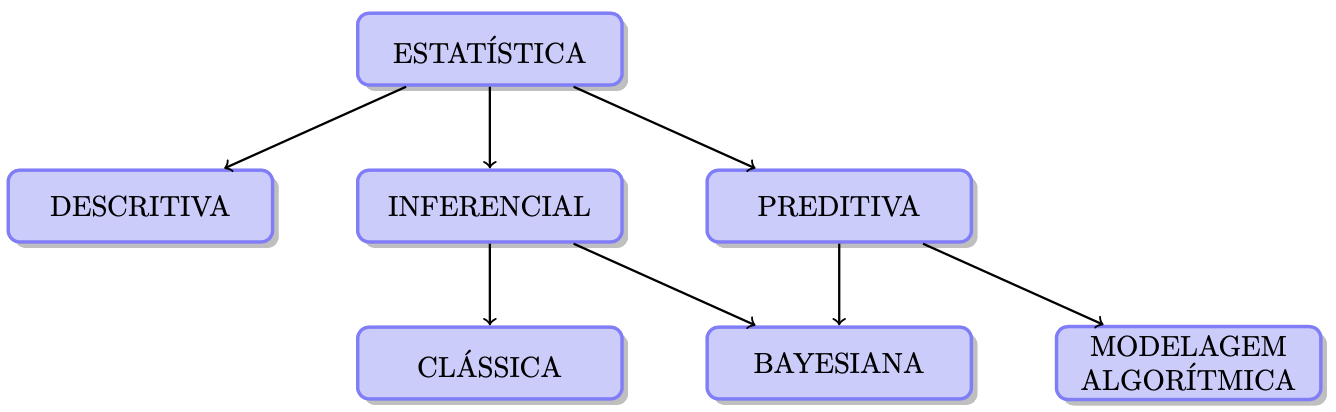
\includegraphics{img/estat.png}
\caption{Uma possível divisão da Estatística.}
\end{figure}

\hypertarget{ferramentas}{%
\section{Ferramentas}\label{ferramentas}}

\hypertarget{r}{%
\subsection{R}\label{r}}

\href{https://www.r-project.org/}{R} é uma ferramenta para cálculos estatísticos e gráficos. Foi desenvolvido no departamento de Estatística da Universidade de Auckland, e seu código está disponível sob a licença \href{https://www.gnu.org/}{GNU} (\emph{GNU is Not Unix}) GPL\footnote{A Licença Pública Geral GNU é um tipo de licença utilizada para software livre, que garante aos usuários finais (indivíduos, organizações ou empresas) a liberdade de usar, estudar, compartilhar e modificar o software.}. Atualmente a \emph{R Foundation} está sediada na Universidade de Economia e Negócios de Viena, Áustria. Foi influenciado por linguagens como \emph{S} e \emph{Scheme} seguindo o conceito minimalista orientado a objeto, que especifica um pequeno núcleo padrão acompanhado de \href{https://cran.r-project.org/web/packages/}{pacotes} para a extensão da linguagem.

Recomenda-se manter o R e seus pacotes sempre atualizados. No Windows recomenda-se ainda a instalação do \href{https://cran.r-project.org/bin/windows/Rtools/}{Rtools} de acordo com a \href{https://cran.r-project.org/bin/windows/Rtools/history.html}{versão} instalada do R. Os pacotes utilizados neste curso podem ser instalados e atualizados conforme código abaixo. No caso de utilização de \href{https://pt.wikipedia.org/wiki/Sistema_operacional_tipo_Unix}{sistema operacional do tipo Unix}, recomenda-se rodar as instruções acima em um \href{https://en.wikipedia.org/wiki/List_of_terminal_emulators}{terminal} após executar o comando \texttt{sudo\ R} seguido da senha do sistema.

\begin{Shaded}
\begin{Highlighting}[]
\NormalTok{packs \textless{}{-}}\StringTok{ }\KeywordTok{c}\NormalTok{(}\StringTok{\textquotesingle{}tidyverse\textquotesingle{}}\NormalTok{,}\StringTok{\textquotesingle{}readxl\textquotesingle{}}\NormalTok{,}\StringTok{\textquotesingle{}e1071\textquotesingle{}}\NormalTok{,}\StringTok{\textquotesingle{}arrangements\textquotesingle{}}\NormalTok{,}\StringTok{\textquotesingle{}DescTools\textquotesingle{}}\NormalTok{,}\StringTok{\textquotesingle{}symmetry\textquotesingle{}}\NormalTok{,}
           \StringTok{\textquotesingle{}mvtnorm\textquotesingle{}}\NormalTok{,}\StringTok{\textquotesingle{}VGAM\textquotesingle{}}\NormalTok{,}\StringTok{\textquotesingle{}chisq.posthoc.test\textquotesingle{}}\NormalTok{,}\StringTok{\textquotesingle{}rgl\textquotesingle{}}\NormalTok{,}\StringTok{\textquotesingle{}ggfortify\textquotesingle{}}\NormalTok{,}\StringTok{\textquotesingle{}factoextra\textquotesingle{}}\NormalTok{,}
           \StringTok{\textquotesingle{}reticulate\textquotesingle{}}\NormalTok{)}
\KeywordTok{install.packages}\NormalTok{(packs, }\DataTypeTok{dep =}\NormalTok{ T)}
\NormalTok{devtools}\OperatorTok{::}\KeywordTok{install\_github}\NormalTok{(}\StringTok{\textquotesingle{}filipezabala/jurimetrics\textquotesingle{}}\NormalTok{, }\DataTypeTok{force=}\NormalTok{T)}
\NormalTok{devtools}\OperatorTok{::}\KeywordTok{install\_github}\NormalTok{(}\StringTok{\textquotesingle{}filipezabala/voice\textquotesingle{}}\NormalTok{, }\DataTypeTok{force=}\NormalTok{T)}
\NormalTok{devtools}\OperatorTok{::}\KeywordTok{install\_github}\NormalTok{(}\StringTok{\textquotesingle{}filipezabala/desempateTecnico\textquotesingle{}}\NormalTok{, }\DataTypeTok{force=}\NormalTok{T)}
\KeywordTok{update.packages}\NormalTok{(}\DataTypeTok{ask =}\NormalTok{ F)}
\end{Highlighting}
\end{Shaded}

\hypertarget{cran-task-views}{%
\subsubsection*{CRAN Task Views}\label{cran-task-views}}
\addcontentsline{toc}{subsubsection}{CRAN Task Views}

As \href{https://cran.r-project.org/web/views/}{CRAN Task Views} visam fornecer informações sobre os pacotes da CRAN (\emph{Comprehensive R Archive Network}) relacionados a um determinado tópico. É recomendado verificar os assuntos de interesse dentro das \href{https://cran.r-project.org/web/views/}{CRAN Task Views} para uma abordagem mais completa utilizando a linguagem R.

\hypertarget{rstudio}{%
\subsection{RStudio}\label{rstudio}}

\href{https://www.rstudio.com/}{RStudio} é um ambiente de desenvolvimento integrado ao R. Possibilita a criação de apresentações e relatórios automáticos em diversos formatos como pdf, html e docx, mesclando linguagens como \href{https://www.r-project.org/}{R}, \href{https://www.latex-project.org/}{LaTeX}, \href{https://www.markdownguide.org/}{markdown}, \href{http://www.open-std.org/jtc1/sc22/wg14/www/docs/n1256.pdf}{C}, \href{http://www.cplusplus.com/}{C++}, \href{https://www.python.org/}{Python}, \href{https://www.mysql.com/}{SQL}, \href{https://html.spec.whatwg.org/}{HTML}, \href{https://www.w3.org/standards/webdesign/htmlcss}{CSS}, \href{https://www.ecma-international.org/ecma-262/11.0/}{JavaScript}, \href{https://mc-stan.org/}{Stan} e \href{https://d3js.org/}{D3}. Está disponível nas edições \href{https://www.rstudio.com/products/rstudio-desktop/}{Desktop}, \href{https://www.rstudio.com/products/rstudio/download-server/}{Server} juntamente com seus respectivos \href{https://www.rstudio.com/products/rstudio/download/preview/}{\emph{previews}}, reunindo as funcionalidades do R de forma parcimoniosa.

\hypertarget{python}{%
\subsection{Python}\label{python}}

\href{https://www.python.org/}{Python} é uma linguagem de programação interpretada, interativa e orientada a objetos. Ela incorpora módulos, exceções, tipagem dinâmica, tipos de dados dinâmicos de nível muito alto e classes. Oferece suporte a vários paradigmas de programação além da programação orientada a objetos, como a programação procedural e funcional. Ele tem interfaces para muitas chamadas de sistema e bibliotecas, bem como para vários sistemas de janela, e é extensível em C ou C ++. Também pode ser usado como uma linguagem de extensão para aplicativos que precisam de uma interface programável. Finalmente, o Python é portátil: ele roda em muitas variantes do Unix, incluindo Linux e macOS, e no Windows.

\hypertarget{python-em-r-markdown}{%
\subsubsection*{Python em R Markdown}\label{python-em-r-markdown}}
\addcontentsline{toc}{subsubsection}{Python em R Markdown}

O pacote \texttt{reticulate} inclui um mecanismo Python para R Markdown que executa trechos de Python em uma única sessão Python incorporada em sua sessão R, permitindo o acesso a objetos criados em trechos de Python do R e vice-versa.

\begin{Shaded}
\begin{Highlighting}[]
\CommentTok{\# Interface de R e Python}
\KeywordTok{library}\NormalTok{(reticulate)}
\KeywordTok{repl\_python}\NormalTok{() }
\end{Highlighting}
\end{Shaded}

\begin{verbatim}
## Python 3.8.5 (/usr/local/bin/python3.8)
## Reticulate 1.18 REPL -- A Python interpreter in R.
\end{verbatim}

\begin{Shaded}
\begin{Highlighting}[]
\NormalTok{os \textless{}{-}}\StringTok{ }\KeywordTok{import}\NormalTok{(}\StringTok{"os"}\NormalTok{)}
\NormalTok{os}\OperatorTok{$}\KeywordTok{listdir}\NormalTok{(}\StringTok{"."}\NormalTok{)}
\end{Highlighting}
\end{Shaded}

\begin{verbatim}
##  [1] "02-descritiva.Rmd"       ".Rhistory"               "01-introducao.Rmd"       ".DS_Store"              
##  [5] "LICENSE"                 "temp.zip"                "index.Rmd"               "_main.tex"              
##  [9] "03-prob.Rmd"             "_main.Rmd"               "07-modelos_lineares.Rmd" "packages.bib"           
## [13] "code"                    "05-inferencia-class.Rmd" "temp.xlsx"               "_main_files"            
## [17] "_bookdown_files"         "README.md"               "06-inferencia-bayes.Rmd" "img"                    
## [21] ".gitignore"              "_main.log"               "09-series_temporais.Rmd" "_book"                  
## [25] "info.R"                  "book.bib"                "08-apr_maquina.Rmd"      "fdepcdd.Rproj"          
## [29] ".git"                    ".Rproj.user"             "10-ref.Rmd"              "04-amostragem.Rmd"
\end{verbatim}

\begin{exercise}
\protect\hypertarget{exr:reticulate}{}{\label{exr:reticulate} }Ler a documentação do \texttt{reticulate} disponível em \url{https://rstudio.github.io/reticulate/}.
\end{exercise}

\hypertarget{jasp}{%
\subsection{JASP}\label{jasp}}

\href{https://jasp-stats.org/}{JASP} é um projeto de código aberto apoiado pela Universidade de Amsterdã. Com interface amigável, oferece procedimentos de análises estatísticas com abordagens clássica e bayesiana. Desenvolvido para análises de publicação, dentre suas principais características, estão:

\begin{itemize}
\tightlist
\item
  Atualização dinâmica de todos os resultados\\
\item
  Layout de planilha e uma interface intuitiva de arrastar e soltar\\
\item
  Saída anotada para comunicar seus resultados\\
\item
  Integração com o \emph{Open Science Framework} (\href{https://osf.io/}{OSF})\\
\item
  Suporte para formato APA (copie gráficos e tabelas diretamente no Word)
\end{itemize}

\hypertarget{stan}{%
\subsection{Stan}\label{stan}}

\href{https://mc-stan.org/}{Stan} é uma plataforma de código aberto para modelagem estatística e computação estatística de alto desempenho. É também utilizado para análise de dados e previsão nas ciências sociais, biológicas e físicas, engenharia e negócios. A biblioteca de matemática de Stan fornece funções de probabilidade e álgebra linear. Pacotes de R adicionais fornecem modelagem linear baseada em expressão, visualização da posteriori e validação cruzada de exclusão. Existem interfaces para diversos ambientes de computação populares, tais como \href{https://mc-stan.org/users/interfaces/rstan.html}{RStan} (R) e \href{https://mc-stan.org/users/interfaces/pystan.html}{PyStan} (Python). Usando a linguagem pode-se obter:

\begin{itemize}
\tightlist
\item
  inferência estatística bayesiana completa com amostragem MCMC (NUTS, HMC)\\
\item
  inferência bayesiana aproximada com inferência variacional (ADVI)\\
\item
  estimativa de máxima verossimilhança penalizada com otimização (L-BFGS)
\end{itemize}

\hypertarget{materiais-de-apoio}{%
\section{Materiais de apoio}\label{materiais-de-apoio}}

\hypertarget{puxe1gina-do-professor-filipe-zabala}{%
\subsection{Página do professor Filipe Zabala}\label{puxe1gina-do-professor-filipe-zabala}}

Em \href{http://filipezabala.com/}{filipezabala.com} o aluno irá encontrar uma série de materiais de apoio como apostilas, vídeos e artigos. Em \href{https://github.com/filipezabala}{github.com/filipezabala} estão disponíveis uma série de repositórios criados pelo professor.

\begin{exercise}
\protect\hypertarget{exr:videoR}{}{\label{exr:videoR} }Para uma introdução aos conceitos básicos de R, assita aos vídeos disponíveis na playlist \href{https://www.youtube.com/playlist?list=PLgnUrXr7_7coSfm067nFXPvShO18o6GQ_}{Ciência de Dados em software livre}.
\end{exercise}

\hypertarget{khan-academy}{%
\subsection{Khan Academy}\label{khan-academy}}

A \href{https://pt.khanacademy.org}{Khan Academy}\footnote{Segundo a informação oficial, `é uma organização sem fins lucrativos com a missão de oferecer uma educação gratuita de alta qualidade para qualquer pessoa, em qualquer lugar'.} possui uma ampla gama de materiais gratuitos em Português, que podem servir de suporte ao aluno durante o curso. A lista a seguir indica os principais fundamentos necessários para o bom desenvolvimento do conteúdo.

\begin{enumerate}
\def\labelenumi{\arabic{enumi}.}
\tightlist
\item
  Propriedades fundamentais de potenciação, radiciação e frações
\end{enumerate}

\begin{itemize}
\tightlist
\item
  \url{https://pt.khanacademy.org/math/brazil-math-grades/pt-5-ano/numeros-fracoes-5ano}~\\
\item
  \url{https://pt.khanacademy.org/math/brazil-math-grades/pt-8-ano/numeros-8ano}
\end{itemize}

\begin{enumerate}
\def\labelenumi{\arabic{enumi}.}
\setcounter{enumi}{1}
\tightlist
\item
  Teoria dos Conjuntos
\end{enumerate}

\begin{itemize}
\tightlist
\item
  \url{https://pt.khanacademy.org/math/6-ano-matematica/numeros-operacoes-com-numeros-naturais-6ano}~\\
\item
  \url{https://pt.khanacademy.org/math/brazil-math-grades/pt-9-ano/numeros-9ano}~\\
\item
  \url{https://pt.khanacademy.org/math/statistics-probability/probability-library\#basic-set-ops}
\end{itemize}

\begin{enumerate}
\def\labelenumi{\arabic{enumi}.}
\setcounter{enumi}{2}
\tightlist
\item
  Análise combinatória e axiomas de probabilidade
\end{enumerate}

\begin{itemize}
\tightlist
\item
  \url{https://pt.khanacademy.org/math/brazil-math-grades/pt-7-ano/probabilidade-e-estatistica-7ano}~\\
\item
  \url{https://pt.khanacademy.org/math/brazil-math-grades/pt-8-ano/probabilidade-e-estatistica-8ano}~\\
\item
  \url{https://pt.khanacademy.org/math/brazil-math-grades/pt-9-ano/probabilidade-e-estistica-9ano}
\end{itemize}

\begin{enumerate}
\def\labelenumi{\arabic{enumi}.}
\setcounter{enumi}{3}
\tightlist
\item
  Funções elementares: linear, polinomial, logarítmica e exponencial
\end{enumerate}

\begin{itemize}
\tightlist
\item
  \url{https://pt.khanacademy.org/math/brazil-math-grades/pt-9-ano/algebra-funcoes-9ano}~\\
\item
  \url{https://pt.khanacademy.org/math/algebra2/exponential-and-logarithmic-functions}
\end{itemize}

\begin{enumerate}
\def\labelenumi{\arabic{enumi}.}
\setcounter{enumi}{4}
\tightlist
\item
  Matrizes, determinantes, decomposições, autovalores e autovetores
\end{enumerate}

\begin{itemize}
\tightlist
\item
  \url{https://pt.khanacademy.org/math/algebra-home/alg-matrices}
\end{itemize}

\begin{enumerate}
\def\labelenumi{\arabic{enumi}.}
\setcounter{enumi}{5}
\tightlist
\item
  Derivadas e integrais
\end{enumerate}

\begin{itemize}
\tightlist
\item
  \url{https://pt.khanacademy.org/math/differential-calculus/dc-diff-intro}~\\
\item
  \url{https://pt.khanacademy.org/math/calculus-home/integration-calc}
\end{itemize}

\hypertarget{algarismos-e-numeros}{%
\section{Algarismos e Números}\label{algarismos-e-numeros}}

Um \emph{algarismo} é um símbolo, enquanto um \emph{número} expressa uma idéia de quantidade. Números são representados por algarismos, sendo fundamental distinguir estes elementos.

\begin{example}
\protect\hypertarget{exm:alg-num}{}{\label{exm:alg-num} }Se há 20 alunos na sala A outros 30 na sala B, pode-se dizer que, em média, há \(\frac{20+30}{2}=25\) alunos nas duas salas. Esta é uma informação numérica. Se rotularmos o sexo masculino como 0 e o feminino como 1, fica claro que 0 e 1 estão sendo tratados como algarismos, uma vez que não expressam quantidades.
\end{example}

\hypertarget{porcentagens-decimais-e-milhares}{%
\section{Porcentagens, Decimais e Milhares}\label{porcentagens-decimais-e-milhares}}

Neste texto será adotado o padrão americano, que utiliza o símbolo de ponto (.) como separador de decimais e vírgula (,) como separador de milhares. Assim, \[\frac{1}{40}  = 0.025 = 0.0250 = .025 = 2.5\% = \frac{2.5}{100}.\] Dízimas periódicas serão escritas na forma \(\frac{1}{3} = 0.333... = 0.\bar{3} \approx 0.333 \approx 0.3\). O número \(32,960 = 30,000 + 2,000 + 960\) deve ser lido como `trinta e dois mil novecentos e sessenta'.\\
Esta opção evita muitos problemas, já que muitos \emph{softwares} estatísticos não são compatíveis com o padrão brasileiro, que utiliza vírgula como separador de decimais e ponto para separar os milhares. Nas anotações pessoais e listas de exercícios poderá ser adotada a notação de preferência do aluno.

\hypertarget{o-senhor-x}{%
\section{\texorpdfstring{O Senhor \(X\)}{O Senhor X}}\label{o-senhor-x}}

Quando avalia-se algo de interesse prático, em geral observam-se nomes longos. Considere a variável

\begin{quote}
\(X\): `número de filhos de mulheres atendidas em um hospital público de Porto Alegre em 2019'.
\end{quote}

Esta longa descrição tornará maçante qualquer texto que utilize-o muitas vezes, tornando impraticável a realização de cálculos envolvendo tal característica de interesse. É razoável, portanto, associar descrições longas a símbolos. A letra \(X\) é famosa por simbolizar algo genérico, tanto na Ciência quanto na vida cotidiana. Note que o símbolo utilizado para separar \(X\) de sua descrição é \texttt{:}, e não \texttt{=}.

Neste texto será utilizado \(X\) (maiúsculo) para representar a característica de interesse, e \(x_k\) (minúsculo) para representar o \(k\)-ésimo valor observado desta característica. Assim, enquanto \(X\) representa genericamente o número de filhos de mulheres atendidas em um hospital público de Porto Alegre em 2019, \(x_4 = 2\) indica que a quarta mulher avaliada no estudo tem dois filhos.

\hypertarget{somatorio}{%
\section{Somatório}\label{somatorio}}

A soma de \(n\) números \(x_1, x_2, ..., x_n\) é representada por \(\sum_{i=1}^n {x_i} = x_1 + x_2 + \dotsb + x_n\), e lê-se `somatório de xis \(i\) de um até ene'.

\begin{example}
\protect\hypertarget{exm:somatorio}{}{\label{exm:somatorio} }(Número de passos) Suponha que foi anotado o `número de passos até a lixeira mais próxima' na cidade de Porto Alegre em \(n = 6\) ocasiões, conforme Tabela a seguir.

\begin{longtable}[]{@{}cccccc@{}}
\toprule
\(x_{1}\) & \(x_{2}\) & \(x_{3}\) & \(x_{4}\) & \(x_{5}\) & \(x_{6}\)\tabularnewline
\midrule
\endhead
186 & 402 & 191 & 20 & 7 & 124\tabularnewline
\bottomrule
\end{longtable}

Esta tabela indica que na primeira ocasião foram caminhados 186 passos até localizar uma lixeira (representado por \(x_1=186\)), na segunda foram 402 passos (representado por \(x_2=402\)), e assim sucessivamente. Para calcular o total de passos caminhados, pode-se fazer
\begin{equation}
\sum_{i=1}^6 {x_i} = x_1 + x_2 + \dotsb + x_6 = 186+402+191+20+7+124 = 930
\label{eq:somatorio}
\end{equation}
\end{example}

\begin{Shaded}
\begin{Highlighting}[]
\DecValTok{186}\OperatorTok{+}\DecValTok{402}\OperatorTok{+}\DecValTok{191}\OperatorTok{+}\DecValTok{20}\OperatorTok{+}\DecValTok{7}\OperatorTok{+}\DecValTok{124}            \CommentTok{\# R e RStudio são calculadoras}
\end{Highlighting}
\end{Shaded}

\begin{verbatim}
## [1] 930
\end{verbatim}

\begin{Shaded}
\begin{Highlighting}[]
\NormalTok{x \textless{}{-}}\StringTok{ }\KeywordTok{c}\NormalTok{(}\DecValTok{186}\NormalTok{,}\DecValTok{402}\NormalTok{,}\DecValTok{191}\NormalTok{,}\DecValTok{20}\NormalTok{,}\DecValTok{7}\NormalTok{,}\DecValTok{124}\NormalTok{)    }\CommentTok{\# Pode{-}se criar um vetor e atribuir a x}
\KeywordTok{sum}\NormalTok{(x)                          }\CommentTok{\# Usando a função \textquotesingle{}sum\textquotesingle{}, apresentada na Equação (1.1)}
\end{Highlighting}
\end{Shaded}

\begin{verbatim}
## [1] 930
\end{verbatim}

\begin{Shaded}
\begin{Highlighting}[]
\KeywordTok{sum}\NormalTok{(x}\OperatorTok{\^{}}\DecValTok{2}\NormalTok{)                        }\CommentTok{\# Soma dos quadrados, representada pela Equação (1.2)}
\end{Highlighting}
\end{Shaded}

\begin{verbatim}
## [1] 248506
\end{verbatim}

A letra grega \(\sum\) é o sigma maiúsculo, conforme Seção \ref{alfabeto-grego}. Em muitos casos a simbologia de somatório é simplificada, utilizando-se \(\sum\), \(\sum_{x}\) ou \(\sum_{i}\). A seguir estão alguns exemplos mais avançados de uso mais sofisticado do somatório, podendo ser omitidos em uma primeira leitura.
\begin{equation}
\sum_{i=1}^n x_{i}^2 = x_{1}^2 + x_{2}^2 + \ldots + x_{n}^2
\label{eq:soma-quad}  
\end{equation}

\begin{exercise}
\protect\hypertarget{exr:corona}{}{\label{exr:corona} }Considere o banco de dados disponível no pacote \texttt{coronavirus}\footnote{\emph{Johns Hopkins University Center for Systems Science and Engineering} (JHU CCSE). \url{https://systems.jhu.edu/research/public-health/ncov}} conforme código a seguir.
\end{exercise}

\begin{Shaded}
\begin{Highlighting}[]
\KeywordTok{library}\NormalTok{(coronavirus)    }\CommentTok{\# chamando a biblioteca \textquotesingle{}coronavirus\textquotesingle{}}
\CommentTok{\# update\_dataset(silence = FALSE)  \# atualizando os dados}
\KeywordTok{data}\NormalTok{(coronavirus)       }\CommentTok{\# deixando o banco de dados disponível}
\KeywordTok{dim}\NormalTok{(coronavirus)        }\CommentTok{\# dimensões do banco de dados (linhas x colunas)}
\end{Highlighting}
\end{Shaded}

\begin{verbatim}
## [1] 219852      7
\end{verbatim}

\begin{Shaded}
\begin{Highlighting}[]
\KeywordTok{head}\NormalTok{(coronavirus)       }\CommentTok{\# mostrando o início do banco de dados}
\end{Highlighting}
\end{Shaded}

\begin{verbatim}
##         date province     country  lat long      type cases
## 1 2020-01-22          Afghanistan 33.9 67.7 confirmed     0
## 2 2020-01-23          Afghanistan 33.9 67.7 confirmed     0
## 3 2020-01-24          Afghanistan 33.9 67.7 confirmed     0
## 4 2020-01-25          Afghanistan 33.9 67.7 confirmed     0
## 5 2020-01-26          Afghanistan 33.9 67.7 confirmed     0
## 6 2020-01-27          Afghanistan 33.9 67.7 confirmed     0
\end{verbatim}

\textbf{a.} Obtenha a soma de casos (\texttt{cases}) registrados ao longo de todo o período.\\
\textbf{b.} Obtenha a soma ao quadrado de casos registrados ao longo de todo o período.\\
\textbf{c.} Obtenha a soma de casos registrados ao longo de todo o período dividido por tipo (\texttt{type}).\\
\textbf{d.} Considerando a variável \(X\): `número de casos registrados' em \texttt{nrow(coronavirus)} linhas do banco de dados, represente os itens a. e b. utilizando a notação de somatório.

\hypertarget{arredondamento-e-truncagem}{%
\section{Arredondamento e Truncagem}\label{arredondamento-e-truncagem}}

\emph{Arredondamento}\footnote{Esta é a regra do \emph{arredondamento para o número mais próximo}.} e \emph{truncagem} são métodos para escrever números com precisão delimitada.

Para \emph{arredondar} um número para a \(k\)-ésima casa decimal, basta observar a \(k\)+1-ésima casa. Se a \(k\)+1-ésima casa decimal for 0, 1, 2, 3 ou 4, mantém-se a \(k\)-ésima casa decimal; se a \(k\)+1-ésima casa decimal for 5, 6, 7, 8 ou 9, soma-se 1 à \(k\)-ésima casa decimal. Como exercício, releia a frase anterior substituindo `\(k\)-ésima' por `primeira' e `\(k\)+1-ésima' por `segunda', aplicando esta regra para o número 153.654321. Note que \textbf{deve-se sempre avaliar o número original para realizar o arredondamento}. Arredondamentos são comuns, por exemplo, ao calcularmos um índice de preço ou um montante de pagamento sobre o qual incidiu certa taxa de juros.

Para \emph{truncar} um número para a \(k\)-ésima casa decimal, basta eliminar a \(k\)+1-ésima casa decimal e suas subsequentes. Como exercício, releia a frase anterior substituindo `\(k\)-ésima' por `primeira' e `\(k\)+1-ésima' por `segunda', aplicando esta regra novamente para o número 153.654321. Compare com os valores arredondados e note que pode-se utilizar números já truncados para continuar a reduzir a precisão sem a necessidade de conhecer o valor original. Truncagens são comuns, por exemplo, para representar idades e ao calcular os graus G1 e G2 da PUCRS. Assim, se o cálculo do seu G1 resultar em 6.99999999, o sistema irá truncar para 6.9, e não arredondar para 7.0.

\begin{example}
\protect\hypertarget{exm:arred-trunc}{}{\label{exm:arred-trunc} }(Arredondamento e truncagem)

\begin{longtable}[]{@{}cll@{}}
\toprule
Decimais & Arredondamento & Truncagem\tabularnewline
\midrule
\endhead
6 & 153.654321 & 153.654321\tabularnewline
5 & 153.65432 & 153.65432\tabularnewline
4 & 153.6543 & 153.6543\tabularnewline
3 & 153.654 & 153.654\tabularnewline
2 & 153.65 & 153.65\tabularnewline
1 & 153.7 & 153.6\tabularnewline
0 & 154 & 153\tabularnewline
-1 & 150 & 150\tabularnewline
-2 & 200 & 100\tabularnewline
\bottomrule
\end{longtable}
\end{example}

\begin{Shaded}
\begin{Highlighting}[]
\CommentTok{\# Usando base R}
\KeywordTok{options}\NormalTok{(}\DataTypeTok{digits =} \DecValTok{10}\NormalTok{)            }\CommentTok{\# Ajustando para apresentação de 10 dígitos (padrão: 7)}
\ControlFlowTok{for}\NormalTok{(i }\ControlFlowTok{in} \DecValTok{6}\OperatorTok{:{-}}\DecValTok{2}\NormalTok{)\{ }\KeywordTok{print}\NormalTok{(}\KeywordTok{round}\NormalTok{(}\FloatTok{153.654321}\NormalTok{, }\DataTypeTok{dig =}\NormalTok{ i)) \}        }\CommentTok{\# \textquotesingle{}digits\textquotesingle{} casas decimais}
\end{Highlighting}
\end{Shaded}

\begin{verbatim}
## [1] 153.654321
## [1] 153.65432
## [1] 153.6543
## [1] 153.654
## [1] 153.65
## [1] 153.7
## [1] 154
## [1] 150
## [1] 200
\end{verbatim}

\begin{Shaded}
\begin{Highlighting}[]
\NormalTok{trunc \textless{}{-}}\StringTok{ }\ControlFlowTok{function}\NormalTok{(x, ..., }\DataTypeTok{dig =} \DecValTok{0}\NormalTok{) base}\OperatorTok{::}\KeywordTok{trunc}\NormalTok{(x}\OperatorTok{*}\DecValTok{10}\OperatorTok{\^{}}\NormalTok{dig, ...)}\OperatorTok{/}\DecValTok{10}\OperatorTok{\^{}}\NormalTok{dig   }\CommentTok{\# Aprimorando}
\ControlFlowTok{for}\NormalTok{(i }\ControlFlowTok{in} \DecValTok{6}\OperatorTok{:{-}}\DecValTok{2}\NormalTok{)\{ }\KeywordTok{print}\NormalTok{(}\KeywordTok{trunc}\NormalTok{(}\FloatTok{153.654321}\NormalTok{, }\DataTypeTok{dig =}\NormalTok{ i)) \}        }\CommentTok{\# Precisão de i decimais}
\end{Highlighting}
\end{Shaded}

\begin{verbatim}
## [1] 153.654321
## [1] 153.65432
## [1] 153.6543
## [1] 153.654
## [1] 153.65
## [1] 153.6
## [1] 153
## [1] 150
## [1] 100
\end{verbatim}

\begin{Shaded}
\begin{Highlighting}[]
\CommentTok{\# Usando o pacote plyr}
\NormalTok{plyr}\OperatorTok{::}\KeywordTok{round\_any}\NormalTok{(}\FloatTok{153.654321}\NormalTok{, }\FloatTok{.01}\NormalTok{, round)           }\CommentTok{\# dig = 2 em round}
\end{Highlighting}
\end{Shaded}

\begin{verbatim}
## [1] 153.65
\end{verbatim}

\begin{Shaded}
\begin{Highlighting}[]
\NormalTok{plyr}\OperatorTok{::}\KeywordTok{round\_any}\NormalTok{(}\FloatTok{153.654321}\NormalTok{, }\FloatTok{.0001}\NormalTok{, floor)         }\CommentTok{\# dig = 4 em trunc}
\end{Highlighting}
\end{Shaded}

\begin{verbatim}
## [1] 153.6543
\end{verbatim}

\begin{Shaded}
\begin{Highlighting}[]
\NormalTok{plyr}\OperatorTok{::}\KeywordTok{round\_any}\NormalTok{(}\FloatTok{153.654321}\NormalTok{, }\DecValTok{1}\NormalTok{, round)             }\CommentTok{\# dig = 0 em round}
\end{Highlighting}
\end{Shaded}

\begin{verbatim}
## [1] 154
\end{verbatim}

\begin{Shaded}
\begin{Highlighting}[]
\NormalTok{plyr}\OperatorTok{::}\KeywordTok{round\_any}\NormalTok{(}\FloatTok{153.654321}\NormalTok{, }\DecValTok{100}\NormalTok{, round)           }\CommentTok{\# dig = {-}2 em round}
\end{Highlighting}
\end{Shaded}

\begin{verbatim}
## [1] 200
\end{verbatim}

\hypertarget{outros}{%
\section{Outros símbolos e expressões}\label{outros}}

\begin{itemize}
\tightlist
\item
  \(\sim\): tem distribuição.
\item
  \(\approx\): aproximadamente.
\item
  \#: número de.
\item
  \(\pm\)/\(\mp\): mais ou menos/menos ou mais.
\item
  \(\bigtriangleup\): fim do Teorema.
\item
  i.e.: \emph{id est}, expressão em Latim que significa `isto é'.
\item
  e.g.: \emph{exempli gratia}, expressão em Latim que significa `por exemplo'.
\end{itemize}

\hypertarget{alfabeto-grego}{%
\subsection{Alfabeto grego}\label{alfabeto-grego}}

\begin{longtable}[]{@{}cclccl@{}}
\toprule
Maiúscula & Minúscula & Nome & Maiúscula & Minúscula & Nome\tabularnewline
\midrule
\endhead
\(A\) & \(\alpha\) & Alfa & \(N\) & \(\nu\) & Nü\tabularnewline
\(B\) & \(\beta\) & Beta & \(\Xi\) & \(\xi\) & Csi\tabularnewline
\(\Gamma\) & \(\gamma\) & Gama & \(O\) & \(o\) & Ômicron\tabularnewline
\(\Delta\) & \(\delta\) & Delta & \(\Pi\) & \(\pi\), \(\varpi\) & Pi\tabularnewline
\(E\) & \(\epsilon\), \(\varepsilon\) & Épsilon & \(P\) & \(\rho\), \(\varrho\) & Rô\tabularnewline
\(Z\) & \(\zeta\) & Zeta & \(\Sigma\) & \(\sigma\), \(\varsigma\) & Sigma\tabularnewline
\(H\) & \(\eta\) & Eta & \(T\) & \(\tau\) & Tau\tabularnewline
\(\Theta\) & \(\theta\), \(\vartheta\) & Teta & \(\Upsilon\) & \(\upsilon\) & Úpsilon\tabularnewline
\(I\) & \(\iota\) & Iota & \(\Phi\) & \(\phi\), \(\varphi\) & Fi\tabularnewline
\(K\) & \(\kappa\), \(\varkappa\) & Capa & \(X\) & \(\chi\) & Qui\tabularnewline
\(\Lambda\) & \(\lambda\) & Lambda & \(\Psi\) & \(\psi\) & Psi\tabularnewline
\(M\) & \(\mu\) & Mü & \(\Omega\) & \(\omega\) & Ômega\tabularnewline
\bottomrule
\end{longtable}

\hypertarget{estatistica-descritiva}{%
\chapter{Estatística Descritiva}\label{estatistica-descritiva}}

A \emph{Estatística Descritiva} está diretamente ligada à organização e descrição dos dados. É utilizada para avaliar como as observações se distribuem, onde estão posicionadas e como se apresentam em termos de dispersão e associação. Neste capítulo serão introduzidos conceitos e métodos descritivos, ponto de partida da \emph{análise exploratória de dados}, passo fundamental para análises estatísticas mais avançadas.

\hypertarget{variuxe1veis}{%
\section{Variáveis}\label{variuxe1veis}}

Variável é uma característica medida nos universos ou amostras. As \emph{variáveis qualitativas} ou \emph{atributos} avaliam características não numéricas no conjunto de interesse, como gênereo, time de futebol e nível de escolaridade. As \emph{variáveis quantitativas} medem características numéricas, como número de alunos prestando atenção ou tempo de uma música em segundos. Podem ser classificadas conforme a Figura a seguir.

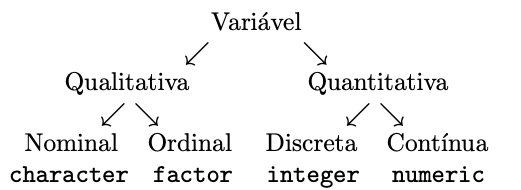
\includegraphics{img/variavel.png}

\hypertarget{variavel-qualitativa-nominal}{%
\subsection{Variável qualitativa nominal}\label{variavel-qualitativa-nominal}}

Variáveis \emph{qualitativas nominais} possuem o menor grau de informação dentre os quatro tipos propostos, permitindo apenas a avaliação de frequências e ordenações arbitrárias. Aplicam-se em avaliações de grupos não ordenados, tais como `gênero', `religião', `raça', `cor preferida', `bairro onde reside', `time de futebol do coração', etc.

\begin{example}
\protect\hypertarget{exm:var-nominal}{}{\label{exm:var-nominal} }(Time de futebol do coração) Suponha um lugar onde tudo seja tratado de maneira dicotômica\footnote{\textit{Dicotomia} é o ato de segmentar um conjunto em dois subconjuntos mutuamente excludentes, i.e., um elemento pode pertencer somente a um dos subconjuntos.}. Como exercício, no primeiro dia de aula de Estatística as pessoas são questionadas quanto ao `time de futebol do coração' através do voto secreto em uma cédula, onde estão listados os dois times locais. Não existe informação prévia que obrigue a dispor na listagem qualquer time antes ou depois de outro. Por este motivo optou-se pela ordenação alfabética -- apesar do princípio de tumulto --, resultando na lista

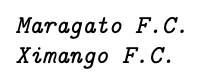
\includegraphics{img/maragato_ximango.png}

Os mais tradicionalistas gritavam palavras de ordem, preferindo a grafia


\includegraphics{img/chimango_maragato.png}
\end{example}

\hypertarget{variavel-qualitativa-ordinal}{%
\subsection{Variável qualitativa ordinal}\label{variavel-qualitativa-ordinal}}

Variáveis \emph{qualitativas ordinais} possuem grau de informação maior em relação às nominais pois são dotadas de uma ordenação prévia, permitindo comparações entre as observações. As variáveis de natureza ordinal são utilizadas quando avaliam-se medidas tais como `colocação em um torneio esportivo', `grau de escolaridade', `classificação de um restaurante quanto à qualidade da comida', etc.

\begin{example}
\protect\hypertarget{exm:var-ordinal1}{}{\label{exm:var-ordinal1} }(Colocação no vestibular) A variável `colocação geral no vestibular' é classificada como qualitativa ordinal pois indica a ordenação do vestibulando em comparação aos demais, mesmo que não se conheça a nota final de cada candidato. \(\\\)
\end{example}

\begin{example}
\protect\hypertarget{exm:var-ordinal2}{}{\label{exm:var-ordinal2} }(Escala de Likert) Quando deseja-se medir o grau de satisfação em relação a algum bem ou serviço, pode-se utilizar a Escala de Likert de \(k\) níveis. Uma vantagem de utilizar \(k\) par é que obriga-se o respondente a se posicionar a favor/contra, acima/abaixo. Se um empresário utilizar \(k=4\), pode fazer 1: Ruim, 2: Regular, 3: Bom, 4: Ótimo. Se \(k=5\), pode-se considerar 1: Péssimo, 2: Ruim, 3: Regular, 4: Bom, 5: Ótimo. \(\\\)
\end{example}

\begin{example}
\protect\hypertarget{exm:var-ordinal3}{}{\label{exm:var-ordinal3} }Corrida maluca) Suponha uma corrida disputada em Imaginationland\footnote{\url{http://www.imdb.com/title/tt0995577}}, na qual Rubinho Barrichello tenha chegado na primeira colocação e Ayrton Senna na décima nona. As únicas informações de que dispomos apontam que i) Barrichello chegou antes de Senna, ii) ninguém chegou antes de Barrichello, iii) há 17 intermediários e iv) de fato, tudo aconteceu em Imaginationland. \(\\\)
\end{example}

\hypertarget{variavel-quantitativa-discreta}{%
\subsection{Variável quantitativa discreta}\label{variavel-quantitativa-discreta}}

Uma variável \emph{quantitativa discreta} assume apenas valores inteiros, i.e., discretos. Tecnicamente as variáveis discretas são caracterizadas por conjuntos enumeráveis\footnote{Um conjunto \textit{enumerável} é aquele em que se pode listar e contar os elementos.} finitos ou infinitos.

\begin{example}
\protect\hypertarget{exm:var-discr1}{}{\label{exm:var-discr1} }(Número de filhos) Suponha que deseja-se observar o número de filhos de mulheres atendidas em um hospital. Para cada mulher entrevistada, o conjunto de possíveis respostas para a pergunta `quantos filhos a senhora tem?' é \(F = \lbrace 0, 1, 2, \ldots, k \rbrace\), onde \(k\) é o número máximo de filhos que uma mulher possa ter ao longo de sua vida. O recorde mundial é \(k=69\), atribuído à russa Valentina Vassilyeva. Este é um conjunto enumerável finito. \(\\\)
\end{example}

\begin{example}
\protect\hypertarget{exm:var-discr2}{}{\label{exm:var-discr2} }(Pontos em um dado lançado \(k\) vezes) Suponha \(k\) lançamentos de um dado. Em cada lançamento é anotada a face resultante, somada aos valores obtidos nos \(k-1\) lançamentos anteriores. O conjunto de possíveis resultados deste experimento é \(S = \lbrace k, k+1, \ldots, 6k \rbrace\). Este é um conjunto enumerável finito. Como exercício, faça \(k=4\) e releia a sentença anterior substituindo os valores. \(\\\)
\end{example}

\begin{example}
\protect\hypertarget{exm:var-discr3}{}{\label{exm:var-discr3} }(Consumo de uma engrenagem moto-contínua) Suponha uma engrenagem eterna, com consumo medido em PAB\footnote{Passos Até a Bufunfa.}. O conjunto do número possível de passos é \(S = \lbrace 1, 2, \ldots \rbrace\). Este é um conjunto enumerável infinito. \(\\\)
\end{example}

\begin{example}
\protect\hypertarget{exm:var-discr4}{}{\label{exm:var-discr4} }(Pilcher's Squad) Norman Pilcher foi o criador da Drug Squad, e ganhou notoriedade nos anos 60 por prender artistas como Mick Jagger e John Lennon. O conjunto de artistas que o Sargento Pilcher poderia prender é \(A = \lbrace a_{1}, a_{2}, \ldots, a_{k} \rbrace\), onde \(k\) representa o número de artistas disponíveis para serem presos. Este é um conjunto enumerável finito. \(\\\)
\end{example}

\hypertarget{variavel-quantitativa-continua}{%
\subsection{Variável quantitativa contínua}\label{variavel-quantitativa-continua}}

A classe de variáveis \emph{quantitativas contínuas} é caracterizada por permitir a observação de qualquer subconjunto dos números reais como resultado, i.e., permite resultados não inteiros. É utilizada para avaliar tempo, distâncias, áreas, volumes ou qualquer outra grandeza numérica de caráter não enumerável\footnote{Um conjunto \emph{não enumerável} possui infinitos elementos, sendo impossível listá-los segundo alguma regra.}. Tal como nas variáveis discretas, é possível avaliar relações matemáticas entre os valores observados.

\begin{example}
\protect\hypertarget{exm:var-cont1}{}{\label{exm:var-cont1} }(Proporção de bulímicas) Suponha que um grupo de pesquisadores está interessado em avaliar a `proporção de mulheres bulímicas no Rio Grande do Sul'. Este valor está obrigatoriamente entre 0 e 1 (ou 0\% e 100\%), podendo ser representado pelo conjunto não enumerável \(\Omega = \lbrace b \in \mathbb{R} : 0 \le b\le 1 \rbrace\). \(\\\)
\end{example}

\begin{example}
\protect\hypertarget{exm:var-cont2}{}{\label{exm:var-cont2} }(Idade) A variável `idade' é classificada como quantitativa contínua por representar uma noção temporal. Caso haja interesse, pode-se dizer que em certo instante do tempo João apresentou \(31.990192013071629871269817323644\) anos de idade. Na prática, porém, geralmente as idades são truncadas, sendo que João provavelmente afirmaria ter 31 anos de idade mesmo um dia antes do seu 32\textordmasculine aniversário. Na melhor das situações as idades são observadas com precisão de dias, calculando-se a idade do indivíduo pela diferença entre o dia de hoje e o seu dia de nascimento, convertendo o valor para anos. O conjunto dos possíveis tempos de vida de um ser humano é dado por \(\Omega = \lbrace t \in \mathbb{R} : 0 < t \le T \rbrace\), onde \(T\) é a idade máxima em anos que um ser humano pode atingir. Segundo o \textit{Guiness World Records}, \(T=122.44931506849315\), alcançado pela francesa Jeanne Louise Calment. \(\Omega\) é dito não enumerável visto não ser possível contabilizar o seu número de elementos. \(\\\)
\end{example}

\begin{example}
\protect\hypertarget{exm:var-cont3}{}{\label{exm:var-cont3} }(Descendo o nível) Suponha que um grupo de pessoas foi avaliado em relação à variável `idade' medida em anos, considerando-se a hora e minuto do nascimento. É possível transformá-la na variável `idade discreta' simplesmente truncando os valores observados. Da mesma forma, pode-se tranformá-la na variável `idade ordinal', classificando-a de acordo com a tabela a seguir.

\begin{longtable}[]{@{}ccc@{}}
\toprule
i & Faixa etária & Classificação\tabularnewline
\midrule
\endhead
1 & Até 10 anos & Criança\tabularnewline
2 & 10 \(\vdash\) 13 & Pré-adolescente\tabularnewline
3 & 13 \(\vdash\) 18 & Adolescente\tabularnewline
4 & 18 \(\vdash\) 35 & Adulto jovem\tabularnewline
5 & 35 \(\vdash\) 45 & Adulto\tabularnewline
6 & 45 \(\vdash\) 65 & Adulto maduro\tabularnewline
7 & 65 \(\vdash\) 75 & Idoso jovem\tabularnewline
8 & 75 + & Idoso\tabularnewline
\bottomrule
\end{longtable}

Note que se uma pessoa tem 31.990192013071629871269817323644 anos de idade (contínua), pode-se considerar a idade truncada de 31 anos (discreta) e classificá-la como um `adulto jovem' (ordinal). Porém, dado que uma pessoa é classificada como adulto jovem, é possível apenas afirmar que ela tem idade entre 18 anos (completos) e 35 anos (incompletos) segundo a classificação proposta. \(\\\)
\end{example}

Cada tipo de variável apresenta um nível de informação que deve ser respeitado. É possível ir de um nível maior de classificação para um nível menor, mas jamais ao contrário. É válido lembrar que perde-se informação ao descer o nível de classificação da variável. É bastante comum, porém, encontrar trabalhos utilizando níveis de classificação inapropriados, conduzindo a técnicas não adequadas que implicam em conclusões equivocadas.

\begin{exercise}
\protect\hypertarget{exr:class-var}{}{\label{exr:class-var} }Classifique as variáveis abaixo (qualitativa nominal/ordinal, quantitativa discreta/contínua).

\begin{enumerate}
\def\labelenumi{\alph{enumi}.}
\tightlist
\item
  Número de geladeiras em casa
\item
  Temperaturas da água da piscina em um dia de verão
\item
  Número de suicídios em uma cidade no decorrer do ano passado
\item
  Concentração de chumbo em uma amostra de água
\item
  Lista de editoras de livros
\item
  Grau de satisfação dos clientes que frequentam uma rinha de galo
\item
  Marcas de amaciantes para roupas
\item
  Tempo que um paciente sobrevive após determinado diagnóstico
\item
  Participação de mercado (\emph{market share})
\item
  Classificação em uma corrida de banheiras
\item
  Tempo final de cada corredor
\item
  Lista dos nomes das banheiras participantes, tal como `Dick Vigarista' e `Trollface'
\item
  Distância de Estambul ao Rio de Janeiro
\end{enumerate}
\end{exercise}

\hypertarget{distribuicao-de-frequencia}{%
\section{Distribuição de Frequência}\label{distribuicao-de-frequencia}}

\hypertarget{db-rol-eo}{%
\subsection{Dados brutos, Rol e Estatísticas de Ordem}\label{db-rol-eo}}

Quando observa-se alguma variável de interesse, em geral anotam-se os resultados na ordem em que aparecem. Esta lista de dados não ordenada é conhecida como \emph{lista de dados brutos}. Quando ordenam-se estes dados -- em ordem crescente ou decrescente -- obtém-se um \emph{rol}, dando origem às \emph{estatísticas de ordem}. Em uma distribuição de \(n\) elementos \(x_{1}\), \(x_{2}\), \(\ldots\), \(x_{n}\) observados sequencialmente, denotam-se os dados ordenados de forma crescente por \(x_{(1)}\), \(x_{(2)}\), \(\ldots\), \(x_{(n)}\) e, analogamente, \(x_{(n)}\), \(x_{(n-1)}\), \(\ldots\), \(x_{(1)}\) para a ordenação decrescente.

\begin{example}
\protect\hypertarget{exm:rol1}{}{\label{exm:rol1} }(Rol) Se ordenarmos os dados observados da variável \(X\):`número de passos até a lixiera mais próxima', obtemos o rol conforme tabela a seguir. O menor número de passos caminhados foi sete, representado por \(x_{(1)}=7\), e o maior foi quatrocentos e dois, representado por \(x_{(6)}=402\).

\begin{longtable}[]{@{}cccccc@{}}
\toprule
\(x_{(1)}\) & \(x_{(2)}\) & \(x_{(3)}\) & \(x_{(4)}\) & \(x_{(5)}\) & \(x_{(6)}\)\tabularnewline
\midrule
\endhead
7 & 20 & 124 & 186 & 191 & 402\tabularnewline
\bottomrule
\end{longtable}
\end{example}

\begin{Shaded}
\begin{Highlighting}[]
\NormalTok{(x \textless{}{-}}\StringTok{ }\KeywordTok{c}\NormalTok{(}\DecValTok{186}\NormalTok{,}\DecValTok{402}\NormalTok{,}\DecValTok{191}\NormalTok{,}\DecValTok{20}\NormalTok{,}\DecValTok{7}\NormalTok{,}\DecValTok{124}\NormalTok{))  }\CommentTok{\# Criando e apresentando o vetor original de dados brutos}
\end{Highlighting}
\end{Shaded}

\begin{verbatim}
## [1] 186 402 191  20   7 124
\end{verbatim}

\begin{Shaded}
\begin{Highlighting}[]
\KeywordTok{sort}\NormalTok{(x)                         }\CommentTok{\# Apresentando o rol, ou vetor ordenado. Teste ?order}
\end{Highlighting}
\end{Shaded}

\begin{verbatim}
## [1]   7  20 124 186 191 402
\end{verbatim}

\begin{Shaded}
\begin{Highlighting}[]
\KeywordTok{sort}\NormalTok{(x, }\DataTypeTok{decreasing =}\NormalTok{ T)         }\CommentTok{\# Ordem decrescente, onde T indica TRUE (padrão: FALSE)}
\end{Highlighting}
\end{Shaded}

\begin{verbatim}
## [1] 402 191 186 124  20   7
\end{verbatim}

Em um primeiro momento estas definições podem parecer ultrapassadas, mas são de grande importância na construção de métodos avançados de análise de dados. Como atualmente trabalham-se com bases de dados em formato eletrônico, em geral é fácil realizar a ordenação de grandes volumes de dados. É importante ressaltar, porém, que em certos casos é necessário muito poder de processamento para executar tais ordenações, podendo se tornarem impraticáveis pelo alto custo computacional.

\begin{exercise}
\protect\hypertarget{exr:rol2}{}{\label{exr:rol2} }Considere o conjunto de dados \(10,-4,5,7,1,3,9\).

\begin{enumerate}
\def\labelenumi{\alph{enumi}.}
\tightlist
\item
  Obtenha o rol.
\item
  Indique e interprete \(x_{(4)}\).
\end{enumerate}
\end{exercise}

\begin{exercise}
\protect\hypertarget{exr:unnamed-chunk-9}{}{\label{exr:unnamed-chunk-9} }Utilizando a função \texttt{sort}, encontre o rol das colunas \texttt{filhos} e \texttt{altura} disponíveis em \url{http://filipezabala.com/data/hospital.txt}.
\end{exercise}

\hypertarget{tab-freq-univ-discr}{%
\subsection{Tabela de frequência univariada discreta}\label{tab-freq-univ-discr}}

Listas muito longas, ainda que ordenadas, não costumam ser de fácil compreensão. Assim, a \emph{tabela de frequência univariada discreta} é uma boa maneira de consolidar os dados de uma variável que assuma, como regra-de-bolso, até 10 diferentes valores. Esta tabela deve apresentar pelo menos uma coluna descrevendo a variável de interesse e uma coluna com a \emph{frequência (da classe)}, i.e., o número de observações contempladas em cada categoria. Sugere-se também a apresentação de uma coluna indicando a classe, denotada por \(i\) conforme Tabela a seguir.

\begin{longtable}[]{@{}cccccccc@{}}
\toprule
\begin{minipage}[b]{0.06\columnwidth}\centering
\(i\)\strut
\end{minipage} & \begin{minipage}[b]{0.06\columnwidth}\centering
\(x_{i}\)\strut
\end{minipage} & \begin{minipage}[b]{0.06\columnwidth}\centering
\(f_{i}\)\strut
\end{minipage} & \begin{minipage}[b]{0.07\columnwidth}\centering
\(f_{r_{i}}\)\strut
\end{minipage} & \begin{minipage}[b]{0.15\columnwidth}\centering
\(F_{i}\)\strut
\end{minipage} & \begin{minipage}[b]{0.07\columnwidth}\centering
\(F_{r_{i}}\)\strut
\end{minipage} & \begin{minipage}[b]{0.20\columnwidth}\centering
\(\Finv_{i}\)\strut
\end{minipage} & \begin{minipage}[b]{0.10\columnwidth}\centering
\(\Finv_{r_{i}}\)\strut
\end{minipage}\tabularnewline
\midrule
\endhead
\begin{minipage}[t]{0.06\columnwidth}\centering
1\strut
\end{minipage} & \begin{minipage}[t]{0.06\columnwidth}\centering
\(x_{1}\)\strut
\end{minipage} & \begin{minipage}[t]{0.06\columnwidth}\centering
\(f_{1}\)\strut
\end{minipage} & \begin{minipage}[t]{0.07\columnwidth}\centering
\(f_{1}/n\)\strut
\end{minipage} & \begin{minipage}[t]{0.15\columnwidth}\centering
\(F_{1}=f_{1}\)\strut
\end{minipage} & \begin{minipage}[t]{0.07\columnwidth}\centering
\(F_{1}/n\)\strut
\end{minipage} & \begin{minipage}[t]{0.20\columnwidth}\centering
\(\Finv_{1}=\Finv_{2}+f_{1}=n\)\strut
\end{minipage} & \begin{minipage}[t]{0.10\columnwidth}\centering
\(\Finv_{1}/n=1\)\strut
\end{minipage}\tabularnewline
\begin{minipage}[t]{0.06\columnwidth}\centering
2\strut
\end{minipage} & \begin{minipage}[t]{0.06\columnwidth}\centering
\(x_{2}\)\strut
\end{minipage} & \begin{minipage}[t]{0.06\columnwidth}\centering
\(f_{2}\)\strut
\end{minipage} & \begin{minipage}[t]{0.07\columnwidth}\centering
\(f_{2}/n\)\strut
\end{minipage} & \begin{minipage}[t]{0.15\columnwidth}\centering
\(F_{2}=F_{1}+f_{2}\)\strut
\end{minipage} & \begin{minipage}[t]{0.07\columnwidth}\centering
\(F_{2}/n\)\strut
\end{minipage} & \begin{minipage}[t]{0.20\columnwidth}\centering
\(\Finv_{2}=\Finv_{3}+f_{2}\)\strut
\end{minipage} & \begin{minipage}[t]{0.10\columnwidth}\centering
\(\Finv_{2}/n\)\strut
\end{minipage}\tabularnewline
\begin{minipage}[t]{0.06\columnwidth}\centering
3\strut
\end{minipage} & \begin{minipage}[t]{0.06\columnwidth}\centering
\(x_{3}\)\strut
\end{minipage} & \begin{minipage}[t]{0.06\columnwidth}\centering
\(f_{3}\)\strut
\end{minipage} & \begin{minipage}[t]{0.07\columnwidth}\centering
\(f_{3}/n\)\strut
\end{minipage} & \begin{minipage}[t]{0.15\columnwidth}\centering
\(F_{3}=F_{2}+f_{3}\)\strut
\end{minipage} & \begin{minipage}[t]{0.07\columnwidth}\centering
\(F_{3}/n\)\strut
\end{minipage} & \begin{minipage}[t]{0.20\columnwidth}\centering
\(\Finv_{3}=\Finv_{4}+f_{3}\)\strut
\end{minipage} & \begin{minipage}[t]{0.10\columnwidth}\centering
\(\Finv_{3}/n\)\strut
\end{minipage}\tabularnewline
\begin{minipage}[t]{0.06\columnwidth}\centering
\(\vdots\)\strut
\end{minipage} & \begin{minipage}[t]{0.06\columnwidth}\centering
\(\vdots\)\strut
\end{minipage} & \begin{minipage}[t]{0.06\columnwidth}\centering
\(\vdots\)\strut
\end{minipage} & \begin{minipage}[t]{0.07\columnwidth}\centering
\(\vdots\)\strut
\end{minipage} & \begin{minipage}[t]{0.15\columnwidth}\centering
\(\vdots\)\strut
\end{minipage} & \begin{minipage}[t]{0.07\columnwidth}\centering
\(\vdots\)\strut
\end{minipage} & \begin{minipage}[t]{0.20\columnwidth}\centering
\(\vdots\)\strut
\end{minipage} & \begin{minipage}[t]{0.10\columnwidth}\centering
\(\vdots\)\strut
\end{minipage}\tabularnewline
\begin{minipage}[t]{0.06\columnwidth}\centering
\(k-2\)\strut
\end{minipage} & \begin{minipage}[t]{0.06\columnwidth}\centering
\(x_{k-2}\)\strut
\end{minipage} & \begin{minipage}[t]{0.06\columnwidth}\centering
\(f_{k-2}\)\strut
\end{minipage} & \begin{minipage}[t]{0.07\columnwidth}\centering
\(f_{k-2}/n\)\strut
\end{minipage} & \begin{minipage}[t]{0.15\columnwidth}\centering
\(F_{k-2}=F_{k-3}+f_{k-2}\)\strut
\end{minipage} & \begin{minipage}[t]{0.07\columnwidth}\centering
\(F_{k-2}/n\)\strut
\end{minipage} & \begin{minipage}[t]{0.20\columnwidth}\centering
\(\Finv_{k-2}=\Finv_{k-1}+f_{k-2}\)\strut
\end{minipage} & \begin{minipage}[t]{0.10\columnwidth}\centering
\(\Finv_{k-2}/n\)\strut
\end{minipage}\tabularnewline
\begin{minipage}[t]{0.06\columnwidth}\centering
\(k-1\)\strut
\end{minipage} & \begin{minipage}[t]{0.06\columnwidth}\centering
\(x_{k-1}\)\strut
\end{minipage} & \begin{minipage}[t]{0.06\columnwidth}\centering
\(f_{k-1}\)\strut
\end{minipage} & \begin{minipage}[t]{0.07\columnwidth}\centering
\(f_{k-1}/n\)\strut
\end{minipage} & \begin{minipage}[t]{0.15\columnwidth}\centering
\(F_{k-1}=F_{k-2}+f_{k-1}\)\strut
\end{minipage} & \begin{minipage}[t]{0.07\columnwidth}\centering
\(F_{k-1}/n\)\strut
\end{minipage} & \begin{minipage}[t]{0.20\columnwidth}\centering
\(\Finv_{k-1}=\Finv_{k}+f_{k-1}\)\strut
\end{minipage} & \begin{minipage}[t]{0.10\columnwidth}\centering
\(\Finv_{k-1}/n\)\strut
\end{minipage}\tabularnewline
\begin{minipage}[t]{0.06\columnwidth}\centering
\(k\)\strut
\end{minipage} & \begin{minipage}[t]{0.06\columnwidth}\centering
\(x_{k}\)\strut
\end{minipage} & \begin{minipage}[t]{0.06\columnwidth}\centering
\(f_{k}\)\strut
\end{minipage} & \begin{minipage}[t]{0.07\columnwidth}\centering
\(f_{k}/n\)\strut
\end{minipage} & \begin{minipage}[t]{0.15\columnwidth}\centering
\(F_{k}=F_{k-1}+f_{k}=n\)\strut
\end{minipage} & \begin{minipage}[t]{0.07\columnwidth}\centering
\(F_{k}/n=1\)\strut
\end{minipage} & \begin{minipage}[t]{0.20\columnwidth}\centering
\(\Finv_{k}=f_{k}\)\strut
\end{minipage} & \begin{minipage}[t]{0.10\columnwidth}\centering
\(\Finv_{k}/n\)\strut
\end{minipage}\tabularnewline
\begin{minipage}[t]{0.06\columnwidth}\centering
Total\strut
\end{minipage} & \begin{minipage}[t]{0.06\columnwidth}\centering
-\strut
\end{minipage} & \begin{minipage}[t]{0.06\columnwidth}\centering
\(n\)\strut
\end{minipage} & \begin{minipage}[t]{0.07\columnwidth}\centering
1\strut
\end{minipage} & \begin{minipage}[t]{0.15\columnwidth}\centering
-\strut
\end{minipage} & \begin{minipage}[t]{0.07\columnwidth}\centering
-\strut
\end{minipage} & \begin{minipage}[t]{0.20\columnwidth}\centering
-\strut
\end{minipage} & \begin{minipage}[t]{0.10\columnwidth}\centering
-\strut
\end{minipage}\tabularnewline
\bottomrule
\end{longtable}

Para a classe genérica \(i\) são calculadas as seguintes frequências:\\
- \(f_{i}\): Frequência (simples/absoluta)\\
- \(f_{r_{i}}\): Frequência relativa\\
- \(F_{i}\): Frequência acumulada\\
- \(F_{r_{i}}\): Frequência acumulada relativa\\
- \(\Finv_{i}\): Frequência acumulada inversa\\
- \(\Finv_{r_{i}}\): Frequência acumulada inversa relativa

\begin{example}
\protect\hypertarget{exm:filhos}{}{\label{exm:filhos} }(Número de filhos revisitado) Do Exemplo \ref{exm:var-discr1} observou-se a variável

\begin{quote}
\(X\): `número de filhos de mulheres atendidas em um hospital de Porto Alegre em 2019'.
\end{quote}

A Tabela a seguir apresenta os dados na ordem em que foram observados. Este tipo de apresentação é bastante completo, mas dificulta a extração de informações relevantes. Como exercício, indique o número máximo de filhos observados na amostra.

\begin{longtable}[]{@{}cccccccccc@{}}
\toprule
\(i\) & \(x_{i}\) & \(i\) & \(x_{i}\) & \(i\) & \(x_{i}\) & \(i\) & \(x_{i}\) & \(i\) & \(x_{i}\)\tabularnewline
\midrule
\endhead
1 & 2 & 21 & 2 & 41 & 1 & 61 & 3 & 81 & 0\tabularnewline
2 & 0 & 22 & 3 & 42 & 1 & 62 & 0 & 82 & 1\tabularnewline
3 & 1 & 23 & 1 & 43 & 4 & 63 & 2 & 83 & 2\tabularnewline
4 & 2 & 24 & 2 & 44 & 1 & 64 & 0 & 84 & 2\tabularnewline
5 & 4 & 25 & 2 & 45 & 1 & 65 & 2 & 85 & 2\tabularnewline
6 & 2 & 26 & 1 & 46 & 3 & 66 & 2 & 86 & 2\tabularnewline
7 & 1 & 27 & 4 & 47 & 1 & 67 & 2 & 87 & 2\tabularnewline
8 & 4 & 28 & 0 & 48 & 1 & 68 & 1 & 88 & 4\tabularnewline
9 & 2 & 29 & 1 & 49 & 4 & 69 & 2 & 89 & 0\tabularnewline
10 & 3 & 30 & 6 & 50 & 2 & 70 & 3 & 90 & 2\tabularnewline
11 & 3 & 31 & 1 & 51 & 2 & 71 & 1 & 91 & 1\tabularnewline
12 & 2 & 32 & 1 & 52 & 4 & 72 & 3 & 92 & 3\tabularnewline
13 & 3 & 33 & 1 & 53 & 1 & 73 & 1 & 93 & 3\tabularnewline
14 & 2 & 34 & 1 & 54 & 3 & 74 & 3 & 94 & 4\tabularnewline
15 & 1 & 35 & 0 & 55 & 1 & 75 & 3 & 95 & 5\tabularnewline
16 & 4 & 36 & 2 & 56 & 2 & 76 & 4 & 96 & 1\tabularnewline
17 & 2 & 37 & 3 & 57 & 0 & 77 & 2 & 97 & 0\tabularnewline
18 & 0 & 38 & 3 & 58 & 2 & 78 & 1 & 98 & 0\tabularnewline
19 & 1 & 39 & 1 & 59 & 3 & 79 & 2 & 99 & 3\tabularnewline
20 & 4 & 40 & 2 & 60 & 3 & 80 & 3 & 100 & 2\tabularnewline
\bottomrule
\end{longtable}
\end{example}

A Tabela a seguir apresenta o número de filhos ordenados, fornecendo ainda algumas frequências que auxiliam o entendimento da distribuição. Com a apresentação neste formato, facilmente observa-se o máximo de 6 filhos na amostra, ao contrário da tabela de dados brutos. Perde-se apenas a ordem na qual os dados foram observados, o que em geral não é do interesse do pesquisador.

\begin{longtable}[]{@{}cccccccc@{}}
\toprule
\(i\) & \(x_{i}\) & \(f_{i}\) & \(f_{r_{i}}\) & \(F_{i}\) & \(F_{r_{i}}\) & \(\Finv_{i}\) & \(\Finv_{r_{i}}\)\tabularnewline
\midrule
\endhead
1 & 0 & 11 & \(11/100=0.11\) & 11 & \(11/100=0.11\) & \(89+11=100\) & \(100/100=1\)\tabularnewline
2 & 1 & 27 & \(27/100=0.27\) & \(11+27=38\) & \(38/100=0.38\) & \(62+27=89\) & \(89/100=0.89\)\tabularnewline
3 & 2 & 30 & \(30/100=0.30\) & \(38+30=68\) & \(68/100=0.68\) & \(32+30=62\) & \(62/100=0.62\)\tabularnewline
4 & 3 & 19 & \(19/100=0.19\) & \(68+19=87\) & \(87/100=0.87\) & \(13+19=32\) & \(32/100=0.32\)\tabularnewline
5 & 4 & 11 & \(11/100=0.11\) & \(87+11=98\) & \(98/100=0.98\) & \(2+11=13\) & \(13/100=0.13\)\tabularnewline
6 & 5 & 1 & \(1/100=0.01\) & \(98+1=99\) & \(99/100=0.99\) & \(1+1=2\) & \(2/100=0.02\)\tabularnewline
7 & 6 & 1 & \(1/100=0.01\) & \(99+1=100\) & \(100/100=1\) & 1 & \(1/100=0.01\)\tabularnewline
Total & - & 100 & 1 & - & - & - & -\tabularnewline
\bottomrule
\end{longtable}

Note que a coluna \(i\) da Tabela acima indica a ordem da mulher entrevistada, enquanto na Tabela de dados brutos \(i\) indica a classe. Por exemplo, \(i=4\) indica a quarta mulher entrevistada, que no caso informou ter \(x_{4}=2\) filhos. Na Tabela acima, \(i=4\) indica a quarta classe onde \(x_{4}=3\), i.e., a classe das mulheres que possuem 3 filhos.

As únicas colunas que exigem a leitura dos dados brutos são a da variável \(x_i\) e a da frequência \(f_i\); as demais são calculadas a partir de \(f_i\). A seguir estão alguns exemplos de interpretação das frequências apresentadas na Tabela acima.\\
- \(f_{5}=11\), i.e., 11 mulheres possuem 4 filhos\\
- \(f_{r_{5}}=0.11=11\%\), i.e., 11\% das mulheres possuem 4 filhos\\
- \(F_{4}=87\), i.e., 87 mulheres possuem até 3 filhos (ou `de zero a 3 filhos', mas esta alternativa é menos elegante)\\
- \(F_{r_{3}}=0.68=68\%\), i.e., 68\% das mulheres possuem até 2 filhos\\
- \(\Finv_{3}=62\), i.e., 62 mulheres têm pelo menos 2 filhos\\
- \(\Finv_{r_{2}}=0.89=89\%\), i.e., 89\% das mulheres têm pelo menos 1 filho

\begin{example}
\protect\hypertarget{exm:filhos-r}{}{\label{exm:filhos-r} }(Número de filhos R-visitado) Exemplo \ref{exm:filhos} utilizando R/RStudio.
\end{example}

\begin{Shaded}
\begin{Highlighting}[]
\NormalTok{hosp \textless{}{-}}\StringTok{ }\KeywordTok{read.table}\NormalTok{(}\StringTok{\textquotesingle{}http://www.filipezabala.com/data/hospital.txt\textquotesingle{}}\NormalTok{, }\DataTypeTok{head =}\NormalTok{ T)}
\KeywordTok{dim}\NormalTok{(hosp)       }\CommentTok{\# Dimensão: 100 linhas por 2 colunas}
\end{Highlighting}
\end{Shaded}

\begin{verbatim}
## [1] 100   2
\end{verbatim}

\begin{Shaded}
\begin{Highlighting}[]
\KeywordTok{head}\NormalTok{(hosp)      }\CommentTok{\# Apresenta as 6 primeiras linhas do objeto \textquotesingle{}hosp\textquotesingle{}; teste tail(hosp, 10)}
\end{Highlighting}
\end{Shaded}

\begin{verbatim}
##   filhos altura
## 1      2   1.59
## 2      0   1.58
## 3      1   1.70
## 4      2   1.62
## 5      4   1.67
## 6      2   1.62
\end{verbatim}

\begin{Shaded}
\begin{Highlighting}[]
\KeywordTok{attach}\NormalTok{(hosp, }\DataTypeTok{warn=}\NormalTok{F)                      }\CommentTok{\# Para deixar as colunas de \textquotesingle{}hosp\textquotesingle{} disponíveis}
\NormalTok{(tab \textless{}{-}}\StringTok{ }\KeywordTok{table}\NormalTok{(filhos))                    }\CommentTok{\# Frequência (simples/absoluta)}
\end{Highlighting}
\end{Shaded}

\begin{verbatim}
## filhos
##  0  1  2  3  4  5  6 
## 11 27 30 19 11  1  1
\end{verbatim}

\begin{Shaded}
\begin{Highlighting}[]
\KeywordTok{prop.table}\NormalTok{(tab)                           }\CommentTok{\# Frequência relativa}
\end{Highlighting}
\end{Shaded}

\begin{verbatim}
## filhos
##    0    1    2    3    4    5    6 
## 0.11 0.27 0.30 0.19 0.11 0.01 0.01
\end{verbatim}

\begin{Shaded}
\begin{Highlighting}[]
\KeywordTok{cumsum}\NormalTok{(tab)                               }\CommentTok{\# Frequência acumulada}
\end{Highlighting}
\end{Shaded}

\begin{verbatim}
##   0   1   2   3   4   5   6 
##  11  38  68  87  98  99 100
\end{verbatim}

\begin{Shaded}
\begin{Highlighting}[]
\KeywordTok{round}\NormalTok{(}\KeywordTok{cumsum}\NormalTok{(tab)}\OperatorTok{/}\KeywordTok{length}\NormalTok{(filhos),}\DecValTok{2}\NormalTok{)       }\CommentTok{\# Frequência acumulada relativa}
\end{Highlighting}
\end{Shaded}

\begin{verbatim}
##    0    1    2    3    4    5    6 
## 0.11 0.38 0.68 0.87 0.98 0.99 1.00
\end{verbatim}

\begin{Shaded}
\begin{Highlighting}[]
\KeywordTok{cumsum}\NormalTok{(}\KeywordTok{rev}\NormalTok{(tab))                          }\CommentTok{\# Frequência acumulada inversa}
\end{Highlighting}
\end{Shaded}

\begin{verbatim}
##   6   5   4   3   2   1   0 
##   1   2  13  32  62  89 100
\end{verbatim}

\begin{Shaded}
\begin{Highlighting}[]
\KeywordTok{round}\NormalTok{(}\KeywordTok{cumsum}\NormalTok{(}\KeywordTok{rev}\NormalTok{(tab))}\OperatorTok{/}\KeywordTok{length}\NormalTok{(filhos),}\DecValTok{2}\NormalTok{)  }\CommentTok{\# Frequência acumulada inversa relativa}
\end{Highlighting}
\end{Shaded}

\begin{verbatim}
##    6    5    4    3    2    1    0 
## 0.01 0.02 0.13 0.32 0.62 0.89 1.00
\end{verbatim}

\begin{exercise}
\protect\hypertarget{exr:ex-tab-fr1}{}{\label{exr:ex-tab-fr1} }Em uma fábrica retirou-se uma amostra de 50 peças de um lote de certo material e contou-se o número de defeitos em cada peça, apresentados na tabela a seguir.

\begin{longtable}[]{@{}cccccccc@{}}
\toprule
\(i\) & \# defeitos & \(f_i\) & \(fr_i\) & \(F_i\) & \(Fr_i\) & \(\Finv_{i}\) & \(\Finv_{r_{i}}\)\tabularnewline
\midrule
\endhead
1 & 0 & 17 & & & & &\tabularnewline
2 & 1 & 10 & & & & &\tabularnewline
3 & 2 & & & & & &\tabularnewline
4 & 3 & 8 & & & & &\tabularnewline
5 & 4 & 5 & & & & &\tabularnewline
6 & 5 & 1 & & & & &\tabularnewline
Total & - & 50 & & & & &\tabularnewline
\bottomrule
\end{longtable}

\begin{enumerate}
\def\labelenumi{\alph{enumi}.}
\tightlist
\item
  Classifique a variável `número de defeitos'.\\
\item
  Qual a frequência absoluta da classe 3? Interprete.\\
\item
  Qual a frequência relativa da classe 3? Interprete.\\
\item
  Qual a frequência acumulada da classe 4? Interprete.\\
\item
  Qual a frequência acumulada relativa da classe 5? Interprete.\\
\item
  Represente os dados utilizando o gráfico que você considerar mais adequado.
\end{enumerate}
\end{exercise}

\hypertarget{tab-freq-univ-cont}{%
\subsection{Tabela de frequência univariada contínua}\label{tab-freq-univ-cont}}

Quando uma variável assume mais de 10 diferentes valores, recomenda-se utilizar a \emph{tabela de frequência univariada contínua}. A diferença para a tabela discreta da Seção \ref{tab-freq-univ-discr} é que na contínua distribuem-se os valores em \emph{intervalos de classe}, i.e., faixas de valores com certa amplitude. A principal vantagem desta abordagem é a capacidade de apresentar os dados de maneira enxuta. O contraponto, como em qualquer resumo de dados, é a perda da informação original.

\hypertarget{amplitude-h-e-quantidade-k-de-classes}{%
\subsubsection*{\texorpdfstring{Amplitude (\(h\)) e quantidade (\(k\)) de classes}{Amplitude (h) e quantidade (k) de classes}}\label{amplitude-h-e-quantidade-k-de-classes}}
\addcontentsline{toc}{subsubsection}{Amplitude (\(h\)) e quantidade (\(k\)) de classes}

Quando deseja-se apresentar a variável em intervalos de classe, é necessário determinar a \emph{amplitude do intervalo de classe} (\(h\)) e a \emph{quantidade de classes} (\(k\)) em que serão dispostos os dados. Apresentam-se a seguir três das principais regras para determinar \(h\) e \(k\).

\hypertarget{sturges}{%
\paragraph*{1. Sturges}\label{sturges}}
\addcontentsline{toc}{paragraph}{1. Sturges}

(Sturges \protect\hyperlink{ref-sturges1926choice}{1926}) sugere que a amplitude do intervalo de classe seja calculada por
\begin{equation}
h_{St} = \frac{A}{k_{St}} = \frac{\max{X}-\min{X}}{1 + \log_{2}{n}} \approx \frac{\max{X}-\min{X}}{1 + 3.322 \log_{10}{n}},
\label{eq:h-sturges}
\end{equation}

onde \(A\) é a \emph{amplitude (dos dados)} descrita na Seção \ref{amplitude}, não devendo ser confundida com \(h\). O denominador é obtido a partir da \emph{expansão binomial}, na forma
\begin{equation}
n = \sum_{i=0}^{k-1} {k-1 \choose i} = (1+1)^{k-1} = 2^{k-1}.
\label{eq:exp-bin}
\end{equation}

Da Equação \eqref{eq:exp-bin} pode-se obter

\begin{equation}
k_{St} = \left\lceil 1 + \log_{2}{n} \right\rceil = \left\lceil 1 + 3.322 \log_{10}{n} \right\rceil,
\label{eq:k-sturges}
\end{equation}

onde \(\left\lceil \;\; \right\rceil\) indica a função \emph{teto}, o menor inteiro consecutivo denotado por \(\left\lceil x \right\rceil = min \{ n \in \mathbb{N} | n \ge x \}\). Alguns pacotes computacionais atribuem o número de classes aplicando regras que encontrem um valor `bonito' para a divisão. Tais valores são obtidos computando números que sejam 0, 1, 2 ou 5 vezes uma potência de 10, i.e., \(a \times 10^b\), \(a \in \{0,1,2,5\}\) e \(b \in \mathbb{N} \cup \{-1\}\).

\begin{example}
\protect\hypertarget{exm:sturges}{}{\label{exm:sturges} }(Sturges) Se forem observados \(n=100\) valores com amplitude (dos dados) \(A=0.23\), a amplitude da classe sugerida por Sturges é \[h_{St} = \frac{0.23}{1 + \log_{2}{100}} = 0.02875,\] e a quantidade de classes \[k_{St} = \left\lceil 1 + \log_{2}{100} \right\rceil = \left\lceil 7.644 \right\rceil = 8.\]
\end{example}

\begin{Shaded}
\begin{Highlighting}[]
\NormalTok{n \textless{}{-}}\StringTok{ }\KeywordTok{length}\NormalTok{(altura)               }\CommentTok{\# n=100, número de dados a serem tabulados}
\NormalTok{A \textless{}{-}}\StringTok{ }\KeywordTok{diff}\NormalTok{(}\KeywordTok{range}\NormalTok{(altura))          }\CommentTok{\# Amplitude (dos dados, não da classe!)}
\KeywordTok{ceiling}\NormalTok{(}\DecValTok{1} \OperatorTok{+}\StringTok{ }\KeywordTok{log2}\NormalTok{(n))              }\CommentTok{\# Pela Equação (2.3), usando log2}
\end{Highlighting}
\end{Shaded}

\begin{verbatim}
## [1] 8
\end{verbatim}

\begin{Shaded}
\begin{Highlighting}[]
\KeywordTok{ceiling}\NormalTok{(}\DecValTok{1} \OperatorTok{+}\StringTok{ }\FloatTok{3.322}\OperatorTok{*}\KeywordTok{log10}\NormalTok{(n))       }\CommentTok{\# Pela Equação (2.3), usando log10}
\end{Highlighting}
\end{Shaded}

\begin{verbatim}
## [1] 8
\end{verbatim}

\begin{Shaded}
\begin{Highlighting}[]
\NormalTok{(kSt \textless{}{-}}\StringTok{ }\KeywordTok{nclass.Sturges}\NormalTok{(altura))   }\CommentTok{\# Pela função \textquotesingle{}nclass.Sturges\textquotesingle{}}
\end{Highlighting}
\end{Shaded}

\begin{verbatim}
## [1] 8
\end{verbatim}

\begin{Shaded}
\begin{Highlighting}[]
\NormalTok{(hSt \textless{}{-}}\StringTok{ }\NormalTok{A}\OperatorTok{/}\NormalTok{kSt)                    }\CommentTok{\# Pela Equação (2.1)}
\end{Highlighting}
\end{Shaded}

\begin{verbatim}
## [1] 0.02875
\end{verbatim}

\begin{Shaded}
\begin{Highlighting}[]
\KeywordTok{pretty}\NormalTok{(kSt)                       }\CommentTok{\# Valores \textquotesingle{}bonitos\textquotesingle{}, (a=5, b=0) e (a=1, b=1)}
\end{Highlighting}
\end{Shaded}

\begin{verbatim}
## [1]  5 10
\end{verbatim}

\hypertarget{scott}{%
\paragraph*{2. Scott}\label{scott}}
\addcontentsline{toc}{paragraph}{2. Scott}

(Scott \protect\hyperlink{ref-scott1979optimal}{1979}) incorpora \(s\), o desvio padrão amostral ao cálculo da amplitude do intervalo, na forma
\begin{equation}
h_{Sc} = \dfrac{3.5s}{n^{1/3}}.
\label{eq:h-scott}
\end{equation}

O número de classes de Scott pode ser obtido por
\begin{equation}
k_{Sc} = \left\lceil \dfrac{A}{h_{Sc}} \right\rceil = \left\lceil \dfrac{max{X} - min{X}}{3.5sn^{-1/3}} \right\rceil.
\label{eq:k-scott}
\end{equation}

\begin{example}
\protect\hypertarget{exm:scott}{}{\label{exm:scott} }(Scott) Se forem observados \(n=100\) valores com desvio padrão amostral \(s=0.045268559\), a amplitude da classe sugerida por Scott é \[h_{Sc} = \dfrac{3.5 \times 0.045268559}{100^{1/3}} = 0.034134854.\] Se \(A=0.23\), a quantidade de classes é \[k_{Sc} =\left\lceil \dfrac{0.23}{0.034134854} \right\rceil = \left\lceil 6.7379811 \right\rceil = 7.\]
\end{example}

\begin{Shaded}
\begin{Highlighting}[]
\NormalTok{n \textless{}{-}}\StringTok{ }\KeywordTok{length}\NormalTok{(altura)                   }\CommentTok{\# n=100, número de observações a serem tabuladas}
\NormalTok{s \textless{}{-}}\StringTok{ }\KeywordTok{sd}\NormalTok{(altura)                       }\CommentTok{\# s=0.045268559, desvio padrão amostral}
\NormalTok{A \textless{}{-}}\StringTok{ }\KeywordTok{diff}\NormalTok{(}\KeywordTok{range}\NormalTok{(altura))              }\CommentTok{\# Amplitude (dos dados, não da classe!)}
\NormalTok{(hSc \textless{}{-}}\StringTok{ }\FloatTok{3.5}\OperatorTok{*}\NormalTok{s}\OperatorTok{/}\NormalTok{n}\OperatorTok{\^{}}\NormalTok{(}\DecValTok{1}\OperatorTok{/}\DecValTok{3}\NormalTok{))                }\CommentTok{\# Pela Equação (2.4)}
\end{Highlighting}
\end{Shaded}

\begin{verbatim}
## [1] 0.03413485378
\end{verbatim}

\begin{Shaded}
\begin{Highlighting}[]
\KeywordTok{ceiling}\NormalTok{(A}\OperatorTok{/}\NormalTok{hSc)                        }\CommentTok{\# k sugerido por Scott, Equação (2.5)}
\end{Highlighting}
\end{Shaded}

\begin{verbatim}
## [1] 7
\end{verbatim}

\begin{Shaded}
\begin{Highlighting}[]
\NormalTok{(kSc \textless{}{-}}\StringTok{ }\KeywordTok{nclass.scott}\NormalTok{(altura))         }\CommentTok{\# k obtido pela função \textquotesingle{}nclass.scott\textquotesingle{}}
\end{Highlighting}
\end{Shaded}

\begin{verbatim}
## [1] 7
\end{verbatim}

\begin{Shaded}
\begin{Highlighting}[]
\KeywordTok{pretty}\NormalTok{(kSc)                           }\CommentTok{\# Valores \textquotesingle{}bonitos\textquotesingle{}, (a=5, b=0) e (a=1, b=1)}
\end{Highlighting}
\end{Shaded}

\begin{verbatim}
## [1]  5 10
\end{verbatim}

\hypertarget{freedman-diaconis}{%
\paragraph*{3. Freedman-Diaconis}\label{freedman-diaconis}}
\addcontentsline{toc}{paragraph}{3. Freedman-Diaconis}

(Freedman and Diaconis \protect\hyperlink{ref-freedman1981histogram}{1981}) inserem a \emph{amplitude interquartílica} no cálculo da amplitude do intervalo, na forma
\begin{equation}
h_{FD} = 2 \dfrac{AI}{n^{1/3}},
\label{eq:h-fd}
\end{equation}

onde \(AI = Q_{3} - Q_{1}\) é a amplitude interquartílica. O número de classes obtido como consequência da aplicação da relação de Freedman-Diaconis é
\begin{equation}
k_{FD} = \left\lceil \dfrac{A}{h_{FD}} \right\rceil = \left\lceil \dfrac{max{X} - min{X}}{2 \, AI \, n^{-1/3}} \right\rceil.
\label{eq:k-fd}
\end{equation}

\begin{example}
\protect\hypertarget{exm:fd}{}{\label{exm:fd} }(Freedman-Diaconis) Se forem observados \(n=100\) valores com amplitude interquartílica de \(AI=0.0525\), a amplitude da classe sugerida por Freedman-Diaconis é \[h_{FD} = \dfrac{2 \times 0.0525}{100^{1/3}} = 0.022621564.\] Se \(A=0.23\), e a quantidade de classes \[k_{FD} = \left\lceil \dfrac{0.23}{0.022621564} \right\rceil = \left\lceil 10.16729 \right\rceil = 11.\]
\end{example}

\begin{Shaded}
\begin{Highlighting}[]
\NormalTok{n \textless{}{-}}\StringTok{ }\KeywordTok{length}\NormalTok{(altura)                   }\CommentTok{\# n=100, número de observações a serem tabuladas}
\NormalTok{(Q \textless{}{-}}\StringTok{ }\KeywordTok{quantile}\NormalTok{(altura, }\KeywordTok{c}\NormalTok{(}\DecValTok{1}\OperatorTok{/}\DecValTok{4}\NormalTok{,}\DecValTok{3}\OperatorTok{/}\DecValTok{4}\NormalTok{)))   }\CommentTok{\# Primeiro e terceiro quartis}
\end{Highlighting}
\end{Shaded}

\begin{verbatim}
##    25%    75% 
## 1.5975 1.6500
\end{verbatim}

\begin{Shaded}
\begin{Highlighting}[]
\NormalTok{(AI \textless{}{-}}\StringTok{ }\KeywordTok{diff}\NormalTok{(}\KeywordTok{as.numeric}\NormalTok{(Q)))     }\CommentTok{\# Amplitude Interquatílica}
\end{Highlighting}
\end{Shaded}

\begin{verbatim}
## [1] 0.0525
\end{verbatim}

\begin{Shaded}
\begin{Highlighting}[]
\NormalTok{(hFD \textless{}{-}}\StringTok{ }\DecValTok{2}\OperatorTok{*}\NormalTok{AI}\OperatorTok{/}\NormalTok{n}\OperatorTok{\^{}}\NormalTok{(}\DecValTok{1}\OperatorTok{/}\DecValTok{3}\NormalTok{))           }\CommentTok{\# Pela Equação (2.6)}
\end{Highlighting}
\end{Shaded}

\begin{verbatim}
## [1] 0.02262156425
\end{verbatim}

\begin{Shaded}
\begin{Highlighting}[]
\NormalTok{A \textless{}{-}}\StringTok{ }\KeywordTok{diff}\NormalTok{(}\KeywordTok{range}\NormalTok{(altura))        }\CommentTok{\# Amplitude (dos dados, não da classe ou interquartílica!)}
\KeywordTok{ceiling}\NormalTok{(A}\OperatorTok{/}\NormalTok{hFD)                  }\CommentTok{\# k sugerido por Freedman{-}Diaconis, Equação (2.7)}
\end{Highlighting}
\end{Shaded}

\begin{verbatim}
## [1] 11
\end{verbatim}

\begin{Shaded}
\begin{Highlighting}[]
\NormalTok{(kFD \textless{}{-}}\StringTok{ }\KeywordTok{nclass.FD}\NormalTok{(altura))      }\CommentTok{\# Pela função \textquotesingle{}nclass.FD\textquotesingle{}}
\end{Highlighting}
\end{Shaded}

\begin{verbatim}
## [1] 11
\end{verbatim}

\begin{Shaded}
\begin{Highlighting}[]
\KeywordTok{pretty}\NormalTok{(kFD)                     }\CommentTok{\# Valores \textquotesingle{}bonitos\textquotesingle{}, (a=1, b=1) e (a=2, b=1)}
\end{Highlighting}
\end{Shaded}

\begin{verbatim}
## [1] 10 20
\end{verbatim}

(Hyndman \protect\hyperlink{ref-hyndman1995problem}{1995}) argumenta que as regras de Scott e Freedman-Diaconis são tão simples quanto a regra de Sturges, mas melhor fundamentadas na teoria estatística. Além disso, a regra de Sturges funciona bem para tamanhos de amostra moderados (\(n < 200\)), mas não para valores grandes de \(n\).

\begin{example}
\protect\hypertarget{exm:hyndman}{}{\label{exm:hyndman} }(Comparando os três métodos) Foi realizada uma simulação com tamanhos de amostra \(n=10^{i}\), \(i \in \{1, 2, \ldots, 6 \}\), indicando o número de classes sugerido por cada método.
\end{example}

\begin{Shaded}
\begin{Highlighting}[]
\NormalTok{NC \textless{}{-}}\StringTok{ }\ControlFlowTok{function}\NormalTok{(x) }\KeywordTok{c}\NormalTok{(}\DataTypeTok{i =}\NormalTok{ i, }\DataTypeTok{n =} \DecValTok{10}\OperatorTok{\^{}}\NormalTok{i,                }\CommentTok{\# Quantidades simuladas}
                    \DataTypeTok{Sturges =} \KeywordTok{nclass.Sturges}\NormalTok{(x),     }\CommentTok{\# Sturges (1926)}
                    \DataTypeTok{Scott =} \KeywordTok{nclass.scott}\NormalTok{(x),         }\CommentTok{\# Scott (1979)}
                    \DataTypeTok{FD =} \KeywordTok{nclass.FD}\NormalTok{(x))               }\CommentTok{\# Freedman{-}Diaconis (1981)}
\ControlFlowTok{for}\NormalTok{(i }\ControlFlowTok{in} \DecValTok{1}\OperatorTok{:}\DecValTok{6}\NormalTok{)\{}\KeywordTok{set.seed}\NormalTok{(i); }\KeywordTok{print}\NormalTok{(}\KeywordTok{NC}\NormalTok{(}\KeywordTok{rnorm}\NormalTok{(}\DecValTok{10}\OperatorTok{\^{}}\NormalTok{i)))\}  }\CommentTok{\# Pode ser demorado para i\textgreater{}6}
\end{Highlighting}
\end{Shaded}

\begin{verbatim}
##       i       n Sturges   Scott      FD 
##       1      10       5       2       3 
##       i       n Sturges   Scott      FD 
##       2     100       8       6       7 
##       i       n Sturges   Scott      FD 
##       3    1000      11      19      25 
##       i       n Sturges   Scott      FD 
##       4   10000      15      44      56 
##       i       n Sturges   Scott      FD 
##       5  100000      18     112     145 
##       i       n Sturges   Scott      FD 
##       6 1000000      21     278     360
\end{verbatim}

\begin{example}
\protect\hypertarget{exm:altura-mulheres}{}{\label{exm:altura-mulheres} }(Alturas de mulheres) Seja a variável

\begin{quote}
\(Y\): `altura de mulheres atendidas em um hospital de Porto Alegre em 2019'.
\end{quote}

A Tabela abaixo apresenta os dados brutos. Este tipo de apresentação é bastante completo, mas dificulta a extração de informações relevantes. Como exercício, indique quantas mulheres têm altura entre 1.70m e 1.75m a partir desta tabela.

\begin{longtable}[]{@{}cccccccc@{}}
\toprule
\(i\) & \(y_{i}\) & \(i\) & \(y_{i}\) & \(i\) & \(y_{i}\) & \(i\) & \(y_{i}\)\tabularnewline
\midrule
\endhead
1 & 1.59 & 26 & 1.61 & 51 & 1.64 & 76 & 1.62\tabularnewline
2 & 1.58 & 27 & 1.61 & 52 & 1.57 & 77 & 1.54\tabularnewline
3 & 1.70 & 28 & 1.60 & 53 & 1.65 & 78 & 1.64\tabularnewline
4 & 1.62 & 29 & 1.61 & 54 & 1.69 & 79 & 1.66\tabularnewline
5 & 1.67 & 30 & 1.64 & 55 & 1.65 & 80 & 1.56\tabularnewline
6 & 1.62 & 31 & 1.59 & 56 & 1.62 & 81 & 1.64\tabularnewline
7 & 1.69 & 32 & 1.60 & 57 & 1.68 & 82 & 1.60\tabularnewline
8 & 1.60 & 33 & 1.62 & 58 & 1.60 & 83 & 1.68\tabularnewline
9 & 1.61 & 34 & 1.53 & 59 & 1.68 & 84 & 1.65\tabularnewline
10 & 1.58 & 35 & 1.58 & 60 & 1.59 & 85 & 1.65\tabularnewline
11 & 1.64 & 36 & 1.60 & 61 & 1.70 & 86 & 1.64\tabularnewline
12 & 1.72 & 37 & 1.61 & 62 & 1.65 & 87 & 1.55\tabularnewline
13 & 1.74 & 38 & 1.67 & 63 & 1.51 & 88 & 1.66\tabularnewline
14 & 1.63 & 39 & 1.68 & 64 & 1.66 & 89 & 1.59\tabularnewline
15 & 1.64 & 40 & 1.56 & 65 & 1.52 & 90 & 1.66\tabularnewline
16 & 1.63 & 41 & 1.58 & 66 & 1.60 & 91 & 1.69\tabularnewline
17 & 1.59 & 42 & 1.66 & 67 & 1.62 & 92 & 1.61\tabularnewline
18 & 1.64 & 43 & 1.59 & 68 & 1.68 & 93 & 1.58\tabularnewline
19 & 1.59 & 44 & 1.67 & 69 & 1.65 & 94 & 1.73\tabularnewline
20 & 1.65 & 45 & 1.62 & 70 & 1.61 & 95 & 1.56\tabularnewline
21 & 1.63 & 46 & 1.55 & 71 & 1.56 & 96 & 1.59\tabularnewline
22 & 1.64 & 47 & 1.64 & 72 & 1.65 & 97 & 1.65\tabularnewline
23 & 1.64 & 48 & 1.62 & 73 & 1.62 & 98 & 1.63\tabularnewline
24 & 1.62 & 49 & 1.65 & 74 & 1.63 & 99 & 1.70\tabularnewline
25 & 1.66 & 50 & 1.66 & 75 & 1.57 & 100 & 1.60\tabularnewline
\bottomrule
\end{longtable}

Para colocar estes valores em uma tabela de frequência, obteve-se \(k_{St}=8\) pela regra de Sturges, e pelo resultado de \texttt{pretty(8)} decidiu-se por 5 classes. Como exercício, obtenha \(k_{Sc}\) e \(k_{FD}\).

A Tabela abaixo apresenta as alturas agrupadas em cinco classes de amplitude 5cm, fornecendo ainda algumas frequências que auxiliam o entendimento da distribuição. Facilmente observam-se 6 mulheres com altura entre 1.70m e 1.75m,\footnote{Note que a simbologia 1.70 \(\vdash\) 1.75 indica a inclusão de 1.70 e a exclusão de 1.75, i.e., este é um intervalo fechado à esquerda e aberto à direita. Equivale às notações \(\left[ 1.70, 1.75 \right[\) (mais moderna) ou \(\left[ 1.70, 1.75 \right)\) (mais antiga).} ao contrário da tabela de dados brutos. Note, porém, que não é possível saber exatamente a altura de cada uma destas 6 mulheres. Isso acontece pois resumo implica em perda de informação, cabendo ao pesquisador decidir quando e como resumir os dados.

\begin{longtable}[]{@{}cccccccc@{}}
\toprule
\(i\) & \(y_{i}\) & \(f_{i}\) & \(f_{r_{i}}\) & \(F_{i}\) & \(F_{r_{i}}\) & \(\Finv_{i}\) & \(\Finv_{r_{i}}\)\tabularnewline
\midrule
\endhead
1 & 1.50 \(\vdash\) 1.55 & 4 & 0.04 & 4 & 0.04 & \(96+4=100\) & \(100/100=1\)\tabularnewline
2 & 1.55 \(\vdash\) 1.60 & 21 & 0.21 & \(4+21=25\) & 0.25 & \(75+21=96\) & \(96/100=0.96\)\tabularnewline
3 & 1.60 \(\vdash\) 1.65 & 41 & 0.41 & \(25+41=66\) & 0.66 & \(34+41=75\) & \(75/100=0.75\)\tabularnewline
4 & 1.65 \(\vdash\) 1.70 & 28 & 0.28 & \(66+28=94\) & 0.94 & \(6+28=34\) & \(34/100=0.34\)\tabularnewline
5 & 1.70 \(\vdash\) 1.75 & 6 & 0.06 & \(94+6=100\) & 1 & 6 & \(6/100=0.06\)\tabularnewline
Total & - & 100 & 1 & - & - & - & -\tabularnewline
\bottomrule
\end{longtable}

A seguir estão alguns exemplos de interpretação das frequências apresentadas na Tabela acima.\\
- \(f_{5}=6\), i.e., 6 mulheres têm entre 1.70m e 1.75m de altura\\
- \(f_{r_{5}}=0.06=6\%\), i.e., 6\% das mulheres tem entre 1.70m e 1.75m de altura\\
- \(F_{4}=94\), i.e., 94 mulheres têm até 1.70m de altura, ou de 1.50m a 1.70m\\
- \(F_{r_{2}}=0.25=25\%\), i.e., 25\% das mulheres tem até 1.60m de altura, ou de 1.50m a 1.60m\\
- \(\Finv_{3}=75\), i.e., 75 mulheres têm pelo menos 1.60m de altura\\
- \(\Finv_{r_{4}}=0.34=34\%\), i.e., 34\% das mulheres tem pelo menos 1.65m de altura \(\\\)
\end{example}

\begin{example}
\protect\hypertarget{exm:altura-mulheres-r}{}{\label{exm:altura-mulheres-r} }(Alturas de mulheres R-visitado) Exemplo \ref{exm:altura-mulheres} utilizando R/RStudio.
\end{example}

\begin{Shaded}
\begin{Highlighting}[]
\NormalTok{hosp \textless{}{-}}\StringTok{ }\KeywordTok{read.table}\NormalTok{(}\StringTok{\textquotesingle{}http://www.filipezabala.com/data/hospital.txt\textquotesingle{}}\NormalTok{, }\DataTypeTok{head =}\NormalTok{ T)}
\KeywordTok{dim}\NormalTok{(hosp)       }\CommentTok{\# Dimensão: 100 linhas por 2 colunas}
\end{Highlighting}
\end{Shaded}

\begin{verbatim}
## [1] 100   2
\end{verbatim}

\begin{Shaded}
\begin{Highlighting}[]
\KeywordTok{head}\NormalTok{(hosp)      }\CommentTok{\# Apresenta as 6 primeiras linhas do objeto \textquotesingle{}hosp\textquotesingle{}; teste tail(hosp, 10)}
\end{Highlighting}
\end{Shaded}

\begin{verbatim}
##   filhos altura
## 1      2   1.59
## 2      0   1.58
## 3      1   1.70
## 4      2   1.62
## 5      4   1.67
## 6      2   1.62
\end{verbatim}

\begin{Shaded}
\begin{Highlighting}[]
\KeywordTok{attach}\NormalTok{(hosp, }\DataTypeTok{warn=}\NormalTok{F)                  }\CommentTok{\# Para deixar as colunas de \textquotesingle{}hosp\textquotesingle{} disponíveis}
\KeywordTok{pretty}\NormalTok{(}\KeywordTok{nclass.Sturges}\NormalTok{(altura))        }\CommentTok{\# Valores \textquotesingle{}bonitos\textquotesingle{} para o número de classes}
\end{Highlighting}
\end{Shaded}

\begin{verbatim}
## [1]  5 10
\end{verbatim}

\begin{Shaded}
\begin{Highlighting}[]
\KeywordTok{hist}\NormalTok{(altura)}\OperatorTok{$}\NormalTok{breaks                   }\CommentTok{\# Quebras de valores gerados com a função \textquotesingle{}hist\textquotesingle{}}
\end{Highlighting}
\end{Shaded}

\begin{verbatim}
## [1] 1.50 1.55 1.60 1.65 1.70 1.75
\end{verbatim}

\begin{Shaded}
\begin{Highlighting}[]
\NormalTok{(f \textless{}{-}}\StringTok{ }\KeywordTok{hist}\NormalTok{(altura)}\OperatorTok{$}\NormalTok{counts)                }\CommentTok{\# Frequências das classes}
\end{Highlighting}
\end{Shaded}

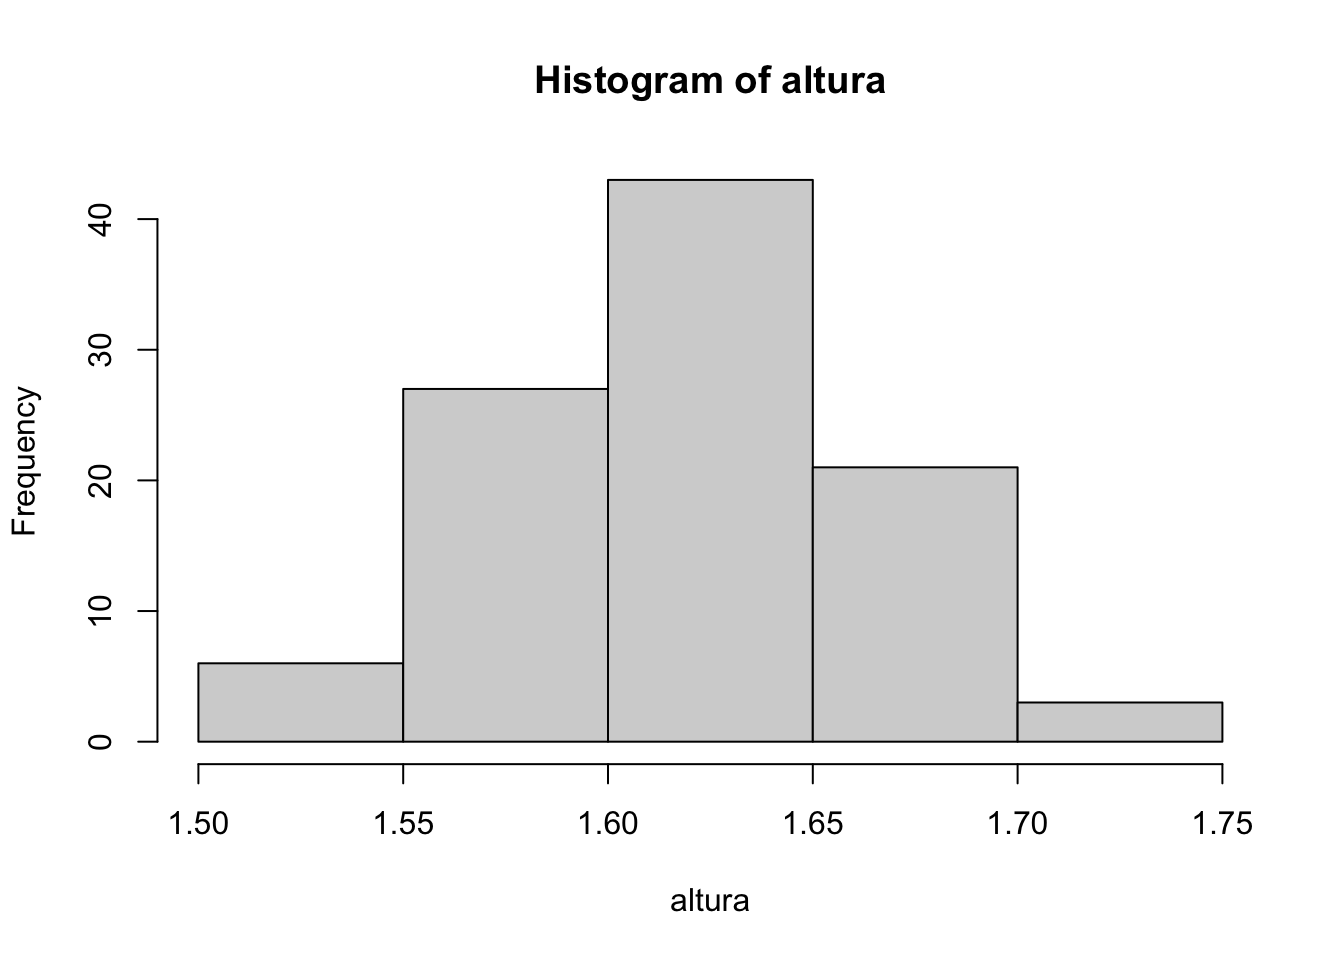
\includegraphics{_main_files/figure-latex/unnamed-chunk-15-1.pdf}

\begin{verbatim}
## [1]  6 27 43 21  3
\end{verbatim}

\begin{Shaded}
\begin{Highlighting}[]
\KeywordTok{cumsum}\NormalTok{(f)                                 }\CommentTok{\# Frequência acumulada}
\end{Highlighting}
\end{Shaded}

\begin{verbatim}
## [1]   6  33  76  97 100
\end{verbatim}

\begin{Shaded}
\begin{Highlighting}[]
\KeywordTok{round}\NormalTok{(}\KeywordTok{cumsum}\NormalTok{(f)}\OperatorTok{/}\KeywordTok{length}\NormalTok{(altura),}\DecValTok{2}\NormalTok{)         }\CommentTok{\# Frequência acumulada relativa}
\end{Highlighting}
\end{Shaded}

\begin{verbatim}
## [1] 0.06 0.33 0.76 0.97 1.00
\end{verbatim}

\begin{Shaded}
\begin{Highlighting}[]
\KeywordTok{cumsum}\NormalTok{(}\KeywordTok{rev}\NormalTok{(f))                            }\CommentTok{\# Frequência acumulada inversa}
\end{Highlighting}
\end{Shaded}

\begin{verbatim}
## [1]   3  24  67  94 100
\end{verbatim}

\begin{Shaded}
\begin{Highlighting}[]
\KeywordTok{round}\NormalTok{(}\KeywordTok{cumsum}\NormalTok{(}\KeywordTok{rev}\NormalTok{(f))}\OperatorTok{/}\KeywordTok{length}\NormalTok{(altura),}\DecValTok{2}\NormalTok{)    }\CommentTok{\# Frequência acumulada inversa relativa}
\end{Highlighting}
\end{Shaded}

\begin{verbatim}
## [1] 0.03 0.24 0.67 0.94 1.00
\end{verbatim}

\hypertarget{posicao}{%
\section{Medidas de Posição (ou Localização)}\label{posicao}}

\hypertarget{minmax}{%
\subsection{Mínimo e Máximo}\label{minmax}}

O \emph{mínimo} de uma distribuição é o menor valor observado desta distribuição; de forma análoga, o \emph{máximo} é o maior valor. São estatísticas de ordem, mais especificamente os extremos de um conjunto de dados ordenado (rol). Para uma distribuição de \(n\) elementos são denotadas por \(\min X = x_{(1)}\) e \(\max X = x_{(n)}\).

Apesar da simplicidade destas medidas, existem considerações teóricas sofisticadas a seu respeito. Para maiores detalhes, vide (Kotz and Nadarajah \protect\hyperlink{ref-kotz2000extreme}{2000}).

\begin{example}
\protect\hypertarget{exm:minmax}{}{\label{exm:minmax} }(Mínimo e máximo) Suponha novamente as \(n=100\) observações da variável Y: `altura de mulheres atendidas em um certo hospital público de Porto Alegre em 2019', apresentadas no Exemplo \ref{exm:altura-mulheres}. O mínimo e o máximo são denotados, respectivamente, por \(\min Y = y_{(1)} = 1.51\) e \(\max Y = y_{(100)} = 1.74\). \(\\\)
\end{example}

\begin{Shaded}
\begin{Highlighting}[]
\KeywordTok{attach}\NormalTok{(}\KeywordTok{read.table}\NormalTok{(}\StringTok{\textquotesingle{}http://www.filipezabala.com/data/hospital.txt\textquotesingle{}}\NormalTok{, }\DataTypeTok{head=}\NormalTok{T), }\DataTypeTok{warn=}\NormalTok{F)}
\KeywordTok{min}\NormalTok{(altura)     }\CommentTok{\# Mínimo}
\end{Highlighting}
\end{Shaded}

\begin{verbatim}
## [1] 1.51
\end{verbatim}

\begin{Shaded}
\begin{Highlighting}[]
\KeywordTok{max}\NormalTok{(altura)     }\CommentTok{\# Máximo}
\end{Highlighting}
\end{Shaded}

\begin{verbatim}
## [1] 1.74
\end{verbatim}

\begin{Shaded}
\begin{Highlighting}[]
\KeywordTok{range}\NormalTok{(altura)   }\CommentTok{\# A função \textquotesingle{}range\textquotesingle{} fornece o mínimo e o máximo}
\end{Highlighting}
\end{Shaded}

\begin{verbatim}
## [1] 1.51 1.74
\end{verbatim}

\hypertarget{mas}{%
\subsection{Média (Aritmética Simples)}\label{mas}}

A \emph{média (aritmética simples)} ou \emph{valor esperado} é uma das medidas mais importantes da Estatística devido às suas propriedades e relativa facilidade de cálculo. A média da variável \(X\) é simbolizada genericamente por \(\mu\) quando refere-se à média universal, e por \(\bar{x}_{n}\) quando refere-se à média amostral. Pode-se utilizar a notação \(\bar{x}_{n}\) para indicar o tamanho da amostra. Suas expressões no universo a na amostra são dadas respectivamente pelas equações \eqref{eq:media-pop} e \eqref{eq:media-am}. Por distribuir a soma dos valores da distribuição pelo número de observações, a média é uma medida que indica centro de massa.
\begin{equation}
\mu = \frac {\sum_{i=1}^N x_i}{N}
\label{eq:media-pop}
\end{equation}

\begin{equation}
\bar{x}_{n} = \frac {\sum_{i=1}^n x_i}{n}
\label{eq:media-am}
\end{equation}

\begin{example}
\protect\hypertarget{exm:media-a-s}{}{\label{exm:media-a-s} }(Média aritmética simples) Suponha novamente os dados do Exemplo \ref{exm:somatorio}. O número médio de passos até a lixeira mais próxima foi de \[\bar{x}_6 = \frac {\sum_{i=1}^6 x_i}{6} = \frac {186+402+191+20+7+124}{6} = \frac{930}{6} = 155.\]\\
\end{example}

\begin{Shaded}
\begin{Highlighting}[]
\NormalTok{x \textless{}{-}}\StringTok{ }\KeywordTok{c}\NormalTok{(}\DecValTok{186}\NormalTok{,}\DecValTok{402}\NormalTok{,}\DecValTok{191}\NormalTok{,}\DecValTok{20}\NormalTok{,}\DecValTok{7}\NormalTok{,}\DecValTok{124}\NormalTok{)      }\CommentTok{\# Vetor de dados brutos}
\KeywordTok{mean}\NormalTok{(x)                           }\CommentTok{\# Aplica as Equações (2.8) e (2.9). Veja ?mean}
\end{Highlighting}
\end{Shaded}

\begin{verbatim}
## [1] 155
\end{verbatim}

\hypertarget{total}{%
\subsection{Total}\label{total}}

\emph{Total} é a soma de todos os valores de uma variável. É expresso pelas equações \eqref{eq:total-pop} e \eqref{eq:total-am}.

\begin{equation}
\tau = \sum_{i=1}^N x_i
\label{eq:total-pop}
\end{equation}

\begin{equation}
\hat{\tau} = \dfrac{N}{n} \sum_{i=1}^n x_i = N \bar{x}_{n},
\label{eq:total-am}
\end{equation}

onde \(\bar{x}_{n}\) é a \emph{média amostral}, apresentada na Equação \eqref{eq:media-am}.

\begin{example}
\protect\hypertarget{exm:total}{}{\label{exm:total} }(Total) Suponha novamente os dados do Exemplo @ref\{exm:media-a-s\}. Se alguém precisar de uma lixeira 20 vezes na capital gaúcha, estima-se que o número total de passos a serem caminhados é de \[\hat{\tau} = \dfrac{20}{6} \times 930 = 20 \times 155 = 3100.\]
\end{example}

\begin{Shaded}
\begin{Highlighting}[]
\NormalTok{N \textless{}{-}}\StringTok{ }\DecValTok{20}                         \CommentTok{\# Tamanho do universo}
\NormalTok{x \textless{}{-}}\StringTok{ }\KeywordTok{c}\NormalTok{(}\DecValTok{186}\NormalTok{,}\DecValTok{402}\NormalTok{,}\DecValTok{191}\NormalTok{,}\DecValTok{20}\NormalTok{,}\DecValTok{7}\NormalTok{,}\DecValTok{124}\NormalTok{)    }\CommentTok{\# Vetor de dados brutos}
\NormalTok{N}\OperatorTok{*}\KeywordTok{mean}\NormalTok{(x)                       }\CommentTok{\# Equação (2.11)}
\end{Highlighting}
\end{Shaded}

\begin{verbatim}
## [1] 3100
\end{verbatim}

\hypertarget{mquadr}{%
\subsection{Média Quadrática}\label{mquadr}}

A \emph{média quadrática} é a média dos valores ao quadrado, utilizada no cálculo das variâncias. É expressa por\\
\begin{equation}
Q^2 = \frac{\sum_{i=1}^n x_{i}^{2}}{n}.
\label{eq:media-quad}
\end{equation}

O \emph{valor quadrático médio} é a raiz quadrada da média quadrática, denotado por
\begin{equation}
Q=\sqrt{Q^2}.
\label{eq:vqm}
\end{equation}

\begin{example}
\protect\hypertarget{exm:mq}{}{\label{exm:mq} }(Média quadrática e valor quadrático médio) A média quadrática dos valores 186, 402, 191, 20, 7 e 124 é \[Q^2 = \frac {\sum_{i=1}^6 x_{i}^{2}}{6} = \frac {186^2+402^2+191^2+20^2+7^2+124^2}{6} = \frac{248506}{6} = 41417.\bar{6}.\] O valor quadrático médio destes valores é \[Q = \sqrt{41417.\bar{6}} \approx 203.5133.\]
\end{example}

\begin{Shaded}
\begin{Highlighting}[]
\NormalTok{x \textless{}{-}}\StringTok{ }\KeywordTok{c}\NormalTok{(}\DecValTok{186}\NormalTok{,}\DecValTok{402}\NormalTok{,}\DecValTok{191}\NormalTok{,}\DecValTok{20}\NormalTok{,}\DecValTok{7}\NormalTok{,}\DecValTok{124}\NormalTok{)    }\CommentTok{\# Vetor de dados brutos}
\NormalTok{(mq \textless{}{-}}\StringTok{ }\KeywordTok{mean}\NormalTok{(x}\OperatorTok{\^{}}\DecValTok{2}\NormalTok{))               }\CommentTok{\# Eq. (2.12), compare com mean(x)\^{}2}
\end{Highlighting}
\end{Shaded}

\begin{verbatim}
## [1] 41417.66667
\end{verbatim}

\begin{Shaded}
\begin{Highlighting}[]
\KeywordTok{sqrt}\NormalTok{(mq)                        }\CommentTok{\# Eq. (2.13), valor quadrático médio}
\end{Highlighting}
\end{Shaded}

\begin{verbatim}
## [1] 203.5133083
\end{verbatim}

\hypertarget{moda}{%
\subsection{Moda}\label{moda}}

A(s) \emph{moda(s)} é (são) o(s) valor(es) mais frequente(s) de uma distribuição. Quando existe apenas uma moda, a distribuição é conhecida como \emph{unimodal}. Se existirem duas modas, a distribuição é \emph{bimodal}. Três modas configuram uma distribuição \emph{trimodal}, e quatro ou mais modas indicam uma distribuição \emph{multimodal}. Distribuições com frequências equivalentes para todos os valores são ditas \emph{amodais}. Quando os dados estão agrupados deve-se indicar a \emph{classe modal}, i.e., a classe de maior frequência. O esforço computacional para calcular a moda é realizar uma contagem.\\
No R existe a função \texttt{Mode} do pacote \texttt{pracma}, mas ela só funciona bem no caso unimodal. Por isso a seguir está apresentada a função \texttt{Modes}, adaptada da sugestão de \href{https://stackoverflow.com/users/316644/digemall}{digEmAll} \href{https://stackoverflow.com/questions/2547402/how-to-find-the-statistical-mode}{nesta discussão do StackOverflow}. Nos exemplos a seguir são comparadas as duas abordagens.

\begin{Shaded}
\begin{Highlighting}[]
\CommentTok{\# Função Modes}
\NormalTok{Modes \textless{}{-}}\StringTok{ }\ControlFlowTok{function}\NormalTok{(x) \{}
\NormalTok{  ux \textless{}{-}}\StringTok{ }\KeywordTok{sort}\NormalTok{(}\KeywordTok{unique}\NormalTok{(x))}
\NormalTok{  tab \textless{}{-}}\StringTok{ }\KeywordTok{tabulate}\NormalTok{(}\KeywordTok{match}\NormalTok{(x, ux))}
\NormalTok{  ux[tab }\OperatorTok{==}\StringTok{ }\KeywordTok{max}\NormalTok{(tab)]}
\NormalTok{\}}
\end{Highlighting}
\end{Shaded}

\begin{example}
\protect\hypertarget{exm:moda1}{}{\label{exm:moda1} }(Unimodal) A moda do conjunto de dados 4, 7, 1, 3, 3, 9 é \(Mo=3\), pois ele apresenta frequência 2 enquanto os demais valores têm frequência 1. Esta é uma distribuição unimodal.
\end{example}

\begin{Shaded}
\begin{Highlighting}[]
\NormalTok{dat \textless{}{-}}\StringTok{ }\KeywordTok{c}\NormalTok{(}\DecValTok{4}\NormalTok{,}\DecValTok{7}\NormalTok{,}\DecValTok{1}\NormalTok{,}\DecValTok{3}\NormalTok{,}\DecValTok{3}\NormalTok{,}\DecValTok{9}\NormalTok{)}
\KeywordTok{Modes}\NormalTok{(dat)}
\end{Highlighting}
\end{Shaded}

\begin{verbatim}
## [1] 3
\end{verbatim}

\begin{Shaded}
\begin{Highlighting}[]
\NormalTok{pracma}\OperatorTok{::}\KeywordTok{Mode}\NormalTok{(dat)}
\end{Highlighting}
\end{Shaded}

\begin{verbatim}
## [1] 3
\end{verbatim}

\begin{example}
\protect\hypertarget{exm:moda2}{}{\label{exm:moda2} }(Bimodal) As modas do conjunto de dados 4, 7, 1, 3, 3, 9, 7 são \(Mo'=3\) e \(Mo''=7\), pois ambos têm frequência 2 enquanto os demais valores têm frequência 1. A ordem de apresentação é indiferente. Esta é uma distribuição bimodal.
\end{example}

\begin{Shaded}
\begin{Highlighting}[]
\NormalTok{dat \textless{}{-}}\StringTok{ }\KeywordTok{c}\NormalTok{(}\DecValTok{4}\NormalTok{,}\DecValTok{7}\NormalTok{,}\DecValTok{1}\NormalTok{,}\DecValTok{3}\NormalTok{,}\DecValTok{3}\NormalTok{,}\DecValTok{9}\NormalTok{,}\DecValTok{7}\NormalTok{)}
\KeywordTok{Modes}\NormalTok{(dat)}
\end{Highlighting}
\end{Shaded}

\begin{verbatim}
## [1] 3 7
\end{verbatim}

\begin{Shaded}
\begin{Highlighting}[]
\NormalTok{pracma}\OperatorTok{::}\KeywordTok{Mode}\NormalTok{(dat)}
\end{Highlighting}
\end{Shaded}

\begin{verbatim}
## [1] 3
\end{verbatim}

\begin{example}
\protect\hypertarget{exm:moda3}{}{\label{exm:moda3} }(Amodal) O conjunto de dados 4, 7, 1, 3, 9 é dito \emph{amodal} pois todos os valores têm frequência 1.
\end{example}

\begin{Shaded}
\begin{Highlighting}[]
\NormalTok{dat \textless{}{-}}\StringTok{ }\KeywordTok{c}\NormalTok{(}\DecValTok{4}\NormalTok{,}\DecValTok{7}\NormalTok{,}\DecValTok{1}\NormalTok{,}\DecValTok{3}\NormalTok{,}\DecValTok{9}\NormalTok{)}
\KeywordTok{Modes}\NormalTok{(dat)    }\CommentTok{\# se todos são moda, ninguém é moda}
\end{Highlighting}
\end{Shaded}

\begin{verbatim}
## [1] 1 3 4 7 9
\end{verbatim}

\begin{Shaded}
\begin{Highlighting}[]
\NormalTok{pracma}\OperatorTok{::}\KeywordTok{Mode}\NormalTok{(dat)}
\end{Highlighting}
\end{Shaded}

\begin{verbatim}
## [1] 1
\end{verbatim}

\begin{example}
\protect\hypertarget{exm:moda4}{}{\label{exm:moda4} }(Moda para dados agrupados) No Exemplo \ref{exm:altura-mulheres} observa-se que \(f_{3}=41\) é a maior frequência. A classe modal é portanto a terceira, compreendida entre os valores 1.60 e 1.65.
\end{example}

\hypertarget{separatrizes}{%
\subsection{Separatrizes}\label{separatrizes}}

Separatrizes ou quantis\footnote{Pronuncia-se \emph{quantís}.} são medidas que dividem um conjunto de dados ordenados em \(k\) partes iguais. O método básico consiste em obter um rol dos dados e encontrar (ainda que de forma aproximada) os valores que repartem a distribuição de acordo com o \(k\) desejado. O esforço computacional para calcular quaisquer separatrizes é, portanto, o de realizar a ordenação dos dados.

\hypertarget{mediana-k2}{%
\subsubsection*{\texorpdfstring{Mediana (\(k=2\))}{Mediana (k=2)}}\label{mediana-k2}}
\addcontentsline{toc}{subsubsection}{Mediana (\(k=2\))}

A \emph{mediana} é a medida que divide metade dos dados ordenados (rol) à sua esquerda e a outra metade à sua direita, i.e., é a medida central em termos de ordenação. Sua posição é a média entre a primeira e última posições, dada por
\begin{equation}
Pos = \frac{1+n}{2}
\label{eq:pos-mediana}
\end{equation}

\begin{example}
\protect\hypertarget{exm:mediana-n-impar}{}{\label{exm:mediana-n-impar} }(Mediana para \(n\) ímpar) Seja o conjunto de dados 10, -4, 11, 12, 1, 5, 15, formado por \(n=7\) valores. Quando ordenado obtemos o rol -4, 1, 5, 10, 11, 12, 15. Considerando \(k=2\), obtém-se a separatriz \(Md=10\), pois ela divide o conjunto em duas partes de mesmo tamanho (três valores abaixo da mediana 10 e três valores acima). Sua posição é dada por \(Pos=\frac{1+7}{2}=4\).
\end{example}

\begin{Shaded}
\begin{Highlighting}[]
\NormalTok{x \textless{}{-}}\StringTok{ }\KeywordTok{c}\NormalTok{(}\DecValTok{10}\NormalTok{, }\DecValTok{{-}4}\NormalTok{, }\DecValTok{11}\NormalTok{, }\DecValTok{12}\NormalTok{, }\DecValTok{1}\NormalTok{, }\DecValTok{5}\NormalTok{, }\DecValTok{15}\NormalTok{)}
\NormalTok{(n \textless{}{-}}\StringTok{ }\KeywordTok{length}\NormalTok{(x))}
\end{Highlighting}
\end{Shaded}

\begin{verbatim}
## [1] 7
\end{verbatim}

\begin{Shaded}
\begin{Highlighting}[]
\NormalTok{(pos \textless{}{-}}\StringTok{ }\NormalTok{(n}\OperatorTok{+}\DecValTok{1}\NormalTok{)}\OperatorTok{/}\DecValTok{2}\NormalTok{)}
\end{Highlighting}
\end{Shaded}

\begin{verbatim}
## [1] 4
\end{verbatim}

\begin{Shaded}
\begin{Highlighting}[]
\KeywordTok{sort}\NormalTok{(x)}
\end{Highlighting}
\end{Shaded}

\begin{verbatim}
## [1] -4  1  5 10 11 12 15
\end{verbatim}

\begin{Shaded}
\begin{Highlighting}[]
\KeywordTok{median}\NormalTok{(x)}
\end{Highlighting}
\end{Shaded}

\begin{verbatim}
## [1] 10
\end{verbatim}

Quando o número de observações é par, basta tomar a média dos dois valores centrais do rol.

\begin{example}
\protect\hypertarget{exm:mediana-n-par}{}{\label{exm:mediana-n-par} }(Mediana para \(n\) par) Seja o conjunto de dados 15, -4, 11, 12, 1, 5, formado por \(n=6\) valores. Quando ordenado obtemos o rol -4, 1, 5, 11, 12, 15. Considerando novamente \(k=2\), obtém-se a separatriz \(Md=\frac{5+11}{2}=8\), pois ela divide o conjunto em duas partes de mesmo tamanho (três valores abaixo de 8 e três valores acima). Sua posição é dada por \(Pos=\frac{1+6}{2}=3.5\), i.e., a mediana é um valor intermediário entre a terceira e quarta posições.
\end{example}

\begin{Shaded}
\begin{Highlighting}[]
\NormalTok{x \textless{}{-}}\StringTok{ }\KeywordTok{c}\NormalTok{(}\DecValTok{15}\NormalTok{, }\DecValTok{{-}4}\NormalTok{, }\DecValTok{11}\NormalTok{, }\DecValTok{12}\NormalTok{, }\DecValTok{1}\NormalTok{, }\DecValTok{5}\NormalTok{)}
\NormalTok{(n \textless{}{-}}\StringTok{ }\KeywordTok{length}\NormalTok{(x))}
\end{Highlighting}
\end{Shaded}

\begin{verbatim}
## [1] 6
\end{verbatim}

\begin{Shaded}
\begin{Highlighting}[]
\NormalTok{(pos \textless{}{-}}\StringTok{ }\NormalTok{(n}\OperatorTok{+}\DecValTok{1}\NormalTok{)}\OperatorTok{/}\DecValTok{2}\NormalTok{)}
\end{Highlighting}
\end{Shaded}

\begin{verbatim}
## [1] 3.5
\end{verbatim}

\begin{Shaded}
\begin{Highlighting}[]
\KeywordTok{sort}\NormalTok{(x)}
\end{Highlighting}
\end{Shaded}

\begin{verbatim}
## [1] -4  1  5 11 12 15
\end{verbatim}

\begin{Shaded}
\begin{Highlighting}[]
\KeywordTok{median}\NormalTok{(x)}
\end{Highlighting}
\end{Shaded}

\begin{verbatim}
## [1] 8
\end{verbatim}

\hypertarget{separatrizes-1}{%
\subsubsection*{Separatrizes}\label{separatrizes-1}}
\addcontentsline{toc}{subsubsection}{Separatrizes}

Pode-se dividir um conjunto de dados em \(k\) setores, sendo os principais apresentados na tabela a seguir

\begin{longtable}[]{@{}ccc@{}}
\toprule
\(k\) & Nome & Simbologia\tabularnewline
\midrule
\endhead
2 & Mediana & Md\tabularnewline
3 & Tercil & \(T_1\), \(T_2\)\tabularnewline
4 & Quartil & \(Q_1\), \(Q_2\), \(Q_3\)\tabularnewline
10 & Decil & \(D_1\), \(D_2\), \(\ldots\), \(D_9\)\tabularnewline
100 & Percentil & \(P_1\), \(P_2\), \(\ldots\), \(P_{99}\)\tabularnewline
\bottomrule
\end{longtable}

\begin{example}
\protect\hypertarget{exm:separatrizes}{}{\label{exm:separatrizes} }(Separatrizes) A função \texttt{quantile} apresenta nove métodos para obtenção de separatrizes, portanto recomenda-se a leitura da documentação para maiores detalhes. Com ela pode-se facilmente obter os quantis desejados, bastando ajustar o argumento \(k\). Note que a função retorna as separatrizes expressas em percentis, onde \(0\%\) equivale ao mínimo e \(100\%\) ao máximo.
\end{example}

\begin{Shaded}
\begin{Highlighting}[]
\NormalTok{hosp \textless{}{-}}\StringTok{ }\KeywordTok{read.table}\NormalTok{(}\StringTok{\textquotesingle{}http://www.filipezabala.com/data/hospital.txt\textquotesingle{}}\NormalTok{, }\DataTypeTok{header =}\NormalTok{ T)}
\KeywordTok{options}\NormalTok{(}\DataTypeTok{digits =} \DecValTok{3}\NormalTok{)                                 }\CommentTok{\# Para melhorar a apresentação}
\KeywordTok{quantile}\NormalTok{(hosp}\OperatorTok{$}\NormalTok{altura, }\DataTypeTok{probs =} \KeywordTok{seq}\NormalTok{(}\DecValTok{0}\NormalTok{, }\DecValTok{1}\NormalTok{, }\DecValTok{1}\OperatorTok{/}\DecValTok{2}\NormalTok{))       }\CommentTok{\# Mediana}
\end{Highlighting}
\end{Shaded}

\begin{verbatim}
##   0%  50% 100% 
## 1.51 1.62 1.74
\end{verbatim}

\begin{Shaded}
\begin{Highlighting}[]
\KeywordTok{quantile}\NormalTok{(hosp}\OperatorTok{$}\NormalTok{altura, }\DataTypeTok{probs =} \KeywordTok{seq}\NormalTok{(}\DecValTok{0}\NormalTok{, }\DecValTok{1}\NormalTok{, }\DecValTok{1}\OperatorTok{/}\DecValTok{3}\NormalTok{))       }\CommentTok{\# Tercis}
\end{Highlighting}
\end{Shaded}

\begin{verbatim}
##    0% 33.3% 66.7%  100% 
##  1.51  1.61  1.65  1.74
\end{verbatim}

\begin{Shaded}
\begin{Highlighting}[]
\KeywordTok{quantile}\NormalTok{(hosp}\OperatorTok{$}\NormalTok{altura, }\DataTypeTok{probs =} \KeywordTok{seq}\NormalTok{(}\DecValTok{0}\NormalTok{, }\DecValTok{1}\NormalTok{, }\DecValTok{1}\OperatorTok{/}\DecValTok{4}\NormalTok{))       }\CommentTok{\# Quartis}
\end{Highlighting}
\end{Shaded}

\begin{verbatim}
##   0%  25%  50%  75% 100% 
## 1.51 1.60 1.62 1.65 1.74
\end{verbatim}

\begin{Shaded}
\begin{Highlighting}[]
\KeywordTok{quantile}\NormalTok{(hosp}\OperatorTok{$}\NormalTok{altura, }\DataTypeTok{probs =} \KeywordTok{seq}\NormalTok{(}\DecValTok{0}\NormalTok{, }\DecValTok{1}\NormalTok{, }\DecValTok{1}\OperatorTok{/}\DecValTok{10}\NormalTok{))      }\CommentTok{\# Decis}
\end{Highlighting}
\end{Shaded}

\begin{verbatim}
##   0%  10%  20%  30%  40%  50%  60%  70%  80%  90% 100% 
## 1.51 1.57 1.59 1.60 1.62 1.62 1.64 1.65 1.66 1.68 1.74
\end{verbatim}

\begin{exercise}
\protect\hypertarget{exr:unnamed-chunk-27}{}{\label{exr:unnamed-chunk-27} }Interprete os quantis do Exemplo \ref{exm:separatrizes}. \(\\\)
\end{exercise}

\begin{exercise}
\protect\hypertarget{exr:unnamed-chunk-28}{}{\label{exr:unnamed-chunk-28} }Considere as separatrizes discutidas nesta Seção.\\
a. Verifique que as separatrizes mediana (Md), segundo quartil (\(Q_2\)) são equivalentes.\\
b. Existem outras medidas equivalentes às do item (a)? Justifique.\\
c.~Considere algum \(k\) diferente dos apresentados e atribua um nome e uma simbologia.\\
d.~Se existem \(k\) `fatias', quantas são as separatrizes? \(\\\)
\end{exercise}

\begin{exercise}
\protect\hypertarget{exr:unnamed-chunk-29}{}{\label{exr:unnamed-chunk-29} }Utilizando a função \texttt{quantile} calcule as separatrizes discutidas nesta Seção com os dados da coluna \texttt{filhos} disponível em \url{http://www.filipezabala.com/data/hospital.txt}.
\end{exercise}

\hypertarget{medidas-de-dispersuxe3o-ou-variabilidade}{%
\section{Medidas de Dispersão (ou Variabilidade)}\label{medidas-de-dispersuxe3o-ou-variabilidade}}

\hypertarget{amplitude}{%
\subsection{Amplitude}\label{amplitude}}

A \emph{amplitude} é a medida de dispersão mais simples de ser calculada, e fornece uma informação rápida sobre a variabilidade do conjunto de dados. É calculada pela expressão
\begin{equation}
A = \max{X} - \min{X}
\label{eq:amplitude}
\end{equation}

\begin{example}
\protect\hypertarget{exm:ampl-termica-pos}{}{\label{exm:ampl-termica-pos} }(Amplitude com valores positivos) A amplitude das temperaturas 6, 4, 9, 20, 7 e 12 é \[A = 20-4 = 16.\] \(\\\)
\end{example}

\begin{Shaded}
\begin{Highlighting}[]
\NormalTok{temp \textless{}{-}}\StringTok{ }\KeywordTok{c}\NormalTok{(}\DecValTok{6}\NormalTok{,}\DecValTok{4}\NormalTok{,}\DecValTok{9}\NormalTok{,}\DecValTok{20}\NormalTok{,}\DecValTok{7}\NormalTok{,}\DecValTok{12}\NormalTok{)  }\CommentTok{\# dados}
\KeywordTok{max}\NormalTok{(temp)}\OperatorTok{{-}}\KeywordTok{min}\NormalTok{(temp)       }\CommentTok{\# pela Eq. (2.15)}
\end{Highlighting}
\end{Shaded}

\begin{verbatim}
## [1] 16
\end{verbatim}

\begin{Shaded}
\begin{Highlighting}[]
\NormalTok{A \textless{}{-}}\StringTok{ }\KeywordTok{range}\NormalTok{(temp)          }\CommentTok{\# a função \textquotesingle{}range\textquotesingle{} retorna o mínimo e o máximo}
\KeywordTok{diff}\NormalTok{(A)                   }\CommentTok{\# a função \textquotesingle{}diff\textquotesingle{} calcula a diferença}
\end{Highlighting}
\end{Shaded}

\begin{verbatim}
## [1] 16
\end{verbatim}

\begin{example}
\protect\hypertarget{exm:ampl-termica-neg}{}{\label{exm:ampl-termica-neg} }(Amplitude com valores negativos) A amplitude das temperaturas 6, -4, 9, 20, 7 e 12 é \[A = 20-(-4) = 24.\] \(\\\)
\end{example}

\begin{Shaded}
\begin{Highlighting}[]
\NormalTok{temp \textless{}{-}}\StringTok{ }\KeywordTok{c}\NormalTok{(}\DecValTok{6}\NormalTok{,}\OperatorTok{{-}}\DecValTok{4}\NormalTok{,}\DecValTok{9}\NormalTok{,}\DecValTok{20}\NormalTok{,}\DecValTok{7}\NormalTok{,}\DecValTok{12}\NormalTok{) }\CommentTok{\# dados}
\KeywordTok{diff}\NormalTok{(}\KeywordTok{range}\NormalTok{(temp))         }\CommentTok{\# funções aninhadas (\textquotesingle{}nested functions\textquotesingle{})}
\end{Highlighting}
\end{Shaded}

\begin{verbatim}
## [1] 24
\end{verbatim}

\hypertarget{variuxe2ncia}{%
\subsection{Variância}\label{variuxe2ncia}}

A \emph{variância} é a principal medida de dispersão da Estatística. É uma média quadrática em relação à média, i.e., avalia o quanto, em média, os dados variam ao quadrado em torno da média. A variância \emph{universal} pode ser calculada pelas Equações \eqref{eq:var-univ1} e \eqref{eq:var-univ2}.

\begin{equation}
\sigma^2 = \frac{\sum_{i=1}^N (x_i - \mu)^2}{N}
\label{eq:var-univ1}
\end{equation}

\begin{equation}
\sigma^2 = \frac{\sum_{i=1}^N x_{i}^2}{N} - \mu^2
\label{eq:var-univ2}
\end{equation}

\begin{example}
\protect\hypertarget{exm:var-univ-descr}{}{\label{exm:var-univ-descr} }A variância universal do conjunto de dados 186, 402, 191, 20, 7 e 124 é\\
\end{example}

\textbf{Equação (2.16)} \[\sigma^2 = \frac{\sum_{i=1}^6 (x_i - 155)^2}{6} = \frac{(186-155)^2+(402-155)^2+ \cdots + (124-155)^2}{6} = \frac{104356}{6} = 17392.\bar{6}\]

\textbf{Equação (2.17)} \[\sigma^2 = \frac{186^2+402^2+191^2+20^2+7^2+124^2}{6} - 155^2 = \frac{248506}{6} - 24025 = 17392.\bar{6}\]

\begin{Shaded}
\begin{Highlighting}[]
\NormalTok{(var.p \textless{}{-}}\StringTok{ }\KeywordTok{var}\NormalTok{(}\KeywordTok{c}\NormalTok{(}\DecValTok{186}\NormalTok{,}\DecValTok{402}\NormalTok{,}\DecValTok{191}\NormalTok{,}\DecValTok{20}\NormalTok{,}\DecValTok{7}\NormalTok{,}\DecValTok{124}\NormalTok{))}\OperatorTok{*}\NormalTok{(}\DecValTok{5}\OperatorTok{/}\DecValTok{6}\NormalTok{))   }\CommentTok{\# variância amostral*(1/fator de correção)}
\end{Highlighting}
\end{Shaded}

\begin{verbatim}
## [1] 17393
\end{verbatim}

A variância \emph{amostral} pode ser calculada pelas Equações \eqref{eq:var-am1} e \eqref{eq:var-am2}

\begin{equation}
\hat{\sigma}^2 = s_{n}^2 = \frac{\sum_{i=1}^n (x_i - \bar{x})^2}{n-1}
\label{eq:var-am1}
\end{equation}

\begin{equation}
\hat{\sigma}^2 = s_{n}^2 = \left( \frac{\sum_{i=1}^n x_{i}^2}{n} - \bar{x}^2 \right) \left( \frac{n}{n-1} \right) 
\label{eq:var-am2}
\end{equation}

\begin{example}
\protect\hypertarget{exm:var-am-descr}{}{\label{exm:var-am-descr} }A variância amostral do conjunto de dados 186, 402, 191, 20, 7 e 124 é\\
\end{example}

\textbf{Equação (2.18)} \[s_{6}^2 = \frac{\sum_{i=1}^6 (x_i - 155)^2}{6-1} = \frac{(186-155)^2+(402-155)^2+ \cdots + (124-155)^2}{6-1} = \frac{104356}{5} = 20871.2\]

\textbf{Equação (2.19)} \[s_{6}^2 = \left( \frac{186^2+402^2+191^2+20^2+7^2+124^2}{6} - 155^2 \right) \left( \frac{6}{5} \right) = 17392.\bar{6} \times 1.2 = 20871.2\]

\begin{Shaded}
\begin{Highlighting}[]
\NormalTok{(var.a \textless{}{-}}\StringTok{ }\KeywordTok{var}\NormalTok{(}\KeywordTok{c}\NormalTok{(}\DecValTok{186}\NormalTok{,}\DecValTok{402}\NormalTok{,}\DecValTok{191}\NormalTok{,}\DecValTok{20}\NormalTok{,}\DecValTok{7}\NormalTok{,}\DecValTok{124}\NormalTok{)))     }\CommentTok{\# \textquotesingle{}var\textquotesingle{} calcula a variância amostral}
\end{Highlighting}
\end{Shaded}

\begin{verbatim}
## [1] 20871
\end{verbatim}

Assim, se o conjunto de dados deste exemplo representar uma amostra observada em 6 vezes que se contou o número de passos até a lixeira mais próxima na capital do Rio Grande (do Sul), pode-se dizer que a variância amostral é 20871.2 passos\(^2\). Dica: não tente interpretar este valor.

Note pela Equação \eqref{eq:var-am1} que a variância amostral é dividida por \(n-1\) e não por \(n\). Isto faz com que a variância amostral seja maior ou igual à variância universal para os mesmos dados. Intuitivamente pode-se pensar como uma espécie de penalidade aplicada a esta medida quando observa-se apenas parte do universo (amostra). Da mesma forma pode-se pensar na variância amostral como o produto entre a variância universal \(\sigma^2\) e o fator \(n/(n-1)\), descrito por

\begin{equation}
s_{n}^2 = \sigma^2 \left( \frac{n}{n-1} \right)
\label{eq:var-univ-am}
\end{equation}

\hypertarget{desvio-padruxe3o}{%
\subsection{Desvio Padrão}\label{desvio-padruxe3o}}

O desvio padrão é a raiz quadrada da variância. O motivo de calcular o desvio padrão é que a sua interpretação é mais intuitiva se comparada à da variância, uma vez que a unidade de medida do desvio padrão é a mesma da variável \(X\). As fórmulas do desvio padrão universal e amostral são dadas respectivamente pelas equações\footnote{Se você ficou confuso com a notação, escreva \(\sigma^2= V\) e \(\sigma=D\) (bem como \(s^2=v\) e \(s=d\)) e repense o problema.} \eqref{eq:dp-univ} e \eqref{eq:dp-am}.

\begin{equation}
\sigma = \sqrt{\sigma^2} 
\label{eq:dp-univ}
\end{equation}

\begin{equation}
s_{n} = \sqrt{s^{2}_{n}}
\label{eq:dp-am}
\end{equation}

\begin{example}
\protect\hypertarget{exm:dp-universal}{}{\label{exm:dp-universal} }(Desvio padrão universal) Do Exemplo \ref{exm:var-univ-descr} sabe-se que a variância universal do conjunto de dados 186, 402, 191, 20, 7 e 124 é \(\sigma^2 = 17392.\bar{6}\). Assim, o desvio padrão universal é \[\sigma = \sqrt{17392.\bar{6}} \approx 131.88126.\]
\end{example}

\begin{Shaded}
\begin{Highlighting}[]
\NormalTok{dat \textless{}{-}}\StringTok{ }\KeywordTok{c}\NormalTok{(}\DecValTok{186}\NormalTok{,}\DecValTok{402}\NormalTok{,}\DecValTok{191}\NormalTok{,}\DecValTok{20}\NormalTok{,}\DecValTok{7}\NormalTok{,}\DecValTok{124}\NormalTok{)    }\CommentTok{\# dados}
\NormalTok{(dp.p \textless{}{-}}\StringTok{ }\KeywordTok{sd}\NormalTok{(dat) }\OperatorTok{*}\StringTok{ }\KeywordTok{sqrt}\NormalTok{(}\DecValTok{5}\OperatorTok{/}\DecValTok{6}\NormalTok{))     }\CommentTok{\# s\_n * raiz(1/fator de correção)}
\end{Highlighting}
\end{Shaded}

\begin{verbatim}
## [1] 132
\end{verbatim}

\begin{Shaded}
\begin{Highlighting}[]
\KeywordTok{all.equal}\NormalTok{(dp.p, }\KeywordTok{sqrt}\NormalTok{(var.p))      }\CommentTok{\# \textquotesingle{}dp.p\textquotesingle{} é igual à raiz quadrada de \textquotesingle{}var.p\textquotesingle{}}
\end{Highlighting}
\end{Shaded}

\begin{verbatim}
## [1] TRUE
\end{verbatim}

\begin{Shaded}
\begin{Highlighting}[]
\KeywordTok{all.equal}\NormalTok{(dp.p}\OperatorTok{\^{}}\DecValTok{2}\NormalTok{, var.p)          }\CommentTok{\# \textquotesingle{}dp.p\textquotesingle{} ao quadrado é igual a \textquotesingle{}var.p\textquotesingle{}}
\end{Highlighting}
\end{Shaded}

\begin{verbatim}
## [1] TRUE
\end{verbatim}

\begin{example}
\protect\hypertarget{exm:dp-amostral}{}{\label{exm:dp-amostral} }Do Exemplo \ref{exm:var-am-descr} sabe-se que a variância amostral do conjunto de dados 186, 402, 191, 20, 7 e 124 é \(s^{2}_{6}= 20871.2\). Assim, o desvio padrão amostral é \[s_{6} = \sqrt{20871.2}  \approx 144.46868.\]
\end{example}

\begin{Shaded}
\begin{Highlighting}[]
\NormalTok{dat \textless{}{-}}\StringTok{ }\KeywordTok{c}\NormalTok{(}\DecValTok{186}\NormalTok{,}\DecValTok{402}\NormalTok{,}\DecValTok{191}\NormalTok{,}\DecValTok{20}\NormalTok{,}\DecValTok{7}\NormalTok{,}\DecValTok{124}\NormalTok{)    }\CommentTok{\# dados}
\NormalTok{(dp.a \textless{}{-}}\StringTok{ }\KeywordTok{sd}\NormalTok{(dat))                 }\CommentTok{\# \textquotesingle{}sd\textquotesingle{} calcula o desvio padrão amostral}
\end{Highlighting}
\end{Shaded}

\begin{verbatim}
## [1] 144
\end{verbatim}

\begin{Shaded}
\begin{Highlighting}[]
\KeywordTok{all.equal}\NormalTok{(dp.a, }\KeywordTok{sqrt}\NormalTok{(var.a))      }\CommentTok{\# \textquotesingle{}dp.a\textquotesingle{} é igual à raiz quadrada de \textquotesingle{}var.a\textquotesingle{}}
\end{Highlighting}
\end{Shaded}

\begin{verbatim}
## [1] TRUE
\end{verbatim}

\begin{Shaded}
\begin{Highlighting}[]
\KeywordTok{all.equal}\NormalTok{(dp.a}\OperatorTok{\^{}}\DecValTok{2}\NormalTok{, var.a)          }\CommentTok{\# \textquotesingle{}dp.a\textquotesingle{} ao quadrado é igual a \textquotesingle{}var.a\textquotesingle{}}
\end{Highlighting}
\end{Shaded}

\begin{verbatim}
## [1] TRUE
\end{verbatim}

Assim, se o conjunto de dados deste exemplo representar uma amostra observada em 6 vezes que se contou o número de passos até a lixeira mais próxima na capital do Rio Grande (do Sul), pode-se dizer que o desvio padrão (amostral, claro) é de aproximadamente 144.5 passos. Pode-se pensar neste valor como uma oscilação média aproximada em torno da média aritmética.

\hypertarget{coeficiente-de-variauxe7uxe3o}{%
\subsection{Coeficiente de variação}\label{coeficiente-de-variauxe7uxe3o}}

O \emph{coeficiente de variação} é uma medida de comparação de variabilidades, uma vez que ajusta o desvio padrão pela média. É preferível ao desvio padrão por ser um número adimensional, i.e., não possui unidade de medida, tornando quaisquer conjuntos de dados comparáveis em termos de variabilidade. É utilizado em diversas áreas da Estatística, mas é popularmente conhecido como medida de risco em carteiras de ativos.

As fórmulas do coeficiente de variação universal e amostral são dadas respectivamente pelas equações \eqref{eq:cv-pop} e \eqref{eq:cv-am}.
\begin{equation}
\gamma = \frac{\sigma}{\mu}
\label{eq:cv-pop}
\end{equation}

\begin{equation}
\hat{\gamma} = g = \frac{s}{\bar{x}}
\label{eq:cv-am}
\end{equation}

\begin{example}
\protect\hypertarget{exm:cv}{}{\label{exm:cv} }(Coeficiente de variação) Duas variáveis são obtidas em um certo experimento químico. A variável X é medida em microgramas e possui média de 0.0045 \(\mu\)g e desvio padrão de 0.0056 \(\mu\)g. A variável Y é medida em mols e possui média de 3549 mols e desvio padrão de 419 mols. O coeficiente de variação de X é dado por \(g_X=\frac{0.0056}{0.0045} \approx 1.24\), e de Y por \(g_Y=\frac{419}{3549} \approx 0.12\). Portanto, como \(1.24 > 0.12\), conclui-se que o conjunto de dados X varia mais do que Y.
\end{example}

\begin{Shaded}
\begin{Highlighting}[]
\NormalTok{mx \textless{}{-}}\StringTok{ }\FloatTok{0.0045}
\NormalTok{dx \textless{}{-}}\StringTok{ }\FloatTok{0.0056}
\KeywordTok{round}\NormalTok{(gx \textless{}{-}}\StringTok{ }\NormalTok{dx}\OperatorTok{/}\NormalTok{mx, }\DecValTok{2}\NormalTok{)   }\CommentTok{\# Coeficiente de variação de X}
\end{Highlighting}
\end{Shaded}

\begin{verbatim}
## [1] 1.24
\end{verbatim}

\begin{Shaded}
\begin{Highlighting}[]
\NormalTok{my \textless{}{-}}\StringTok{ }\DecValTok{3549}
\NormalTok{dy \textless{}{-}}\StringTok{ }\DecValTok{419}
\KeywordTok{round}\NormalTok{(gy \textless{}{-}}\StringTok{ }\NormalTok{dy}\OperatorTok{/}\NormalTok{my, }\DecValTok{2}\NormalTok{)   }\CommentTok{\# Coeficiente de variação de Y}
\end{Highlighting}
\end{Shaded}

\begin{verbatim}
## [1] 0.12
\end{verbatim}

\hypertarget{outras-medidas}{%
\section{Outras medidas}\label{outras-medidas}}

\hypertarget{assimetria-ou-obliquidade}{%
\subsection{Assimetria (ou Obliquidade)}\label{assimetria-ou-obliquidade}}

\emph{Assimetria} ou \emph{obliquidade} é uma medida que avalia a assimetria de uma distribuição de frequência. Existem diversas definições na literatura, das quais apresentam-se três alternativas.
\begin{equation}
g_1 = \dfrac{m_3}{m_2^{3/2}} = \dfrac{\frac{1}{n} \sum_{i=1}^{n} (x_{i} - \bar{x}_n)^3}{\left[ \frac{1}{n} \sum_{i=1}^{n} (x_{i} - \bar{x}_n)^2 \right]^{3/2}}
\label{eq:ass1}
\end{equation}

\begin{equation}
b_1 = g_{1} \left( \dfrac{n-1}{n} \right)^{3/2} = \dfrac{m_3}{s^3} = \dfrac{\frac{1}{n} \sum_{i=1}^{n} (x_{i} - \bar{x}_n)^3 }{\left[ \frac{1}{n-1} \sum_{i=1}^{n} (x_{i} - \bar{x}_n)^2 \right]^{3/2}}
\label{eq:ass3}
\end{equation}

\begin{eqnarray}
G_1 = g_{1} \sqrt{\dfrac{n(n-1)}{n-2}} = b_{1} \dfrac{n^2}{(n-1)(n-2)}
\label{eq:ass2}
\end{eqnarray}

\begin{Shaded}
\begin{Highlighting}[]
\KeywordTok{set.seed}\NormalTok{(}\DecValTok{1}\NormalTok{); x \textless{}{-}}\StringTok{ }\KeywordTok{rnorm}\NormalTok{(}\DecValTok{100}\NormalTok{)    }\CommentTok{\# Gerando 100 valores N(0,1) com semente fixa}
\NormalTok{e1071}\OperatorTok{::}\KeywordTok{skewness}\NormalTok{(x, }\DataTypeTok{type =} \DecValTok{1}\NormalTok{)    }\CommentTok{\# Definição clássica de assimetria, Equação (2.25)}
\end{Highlighting}
\end{Shaded}

\begin{verbatim}
## [1] -0.0722
\end{verbatim}

\begin{Shaded}
\begin{Highlighting}[]
\NormalTok{e1071}\OperatorTok{::}\KeywordTok{skewness}\NormalTok{(x, }\DataTypeTok{type =} \DecValTok{2}\NormalTok{)    }\CommentTok{\# Utilizada no SAS, SPSS e Excel, Equação (2.27)}
\end{Highlighting}
\end{Shaded}

\begin{verbatim}
## [1] -0.0733
\end{verbatim}

\begin{Shaded}
\begin{Highlighting}[]
\NormalTok{e1071}\OperatorTok{::}\KeywordTok{skewness}\NormalTok{(x, }\DataTypeTok{type =} \DecValTok{3}\NormalTok{)    }\CommentTok{\# Padrão do R, utilizada no MINITAB e BMDP, Equação (2.26)}
\end{Highlighting}
\end{Shaded}

\begin{verbatim}
## [1] -0.0712
\end{verbatim}

\hypertarget{curtose}{%
\subsection{Curtose}\label{curtose}}

A \emph{curtose} é uma medida de achatamento de uma distribuição de frequência. Assim como na assimetria, das diversas definições de curtose apresentam-se três alternativas.
\begin{eqnarray}
g_2 = \dfrac{m_4}{m_2^{2}} - 3 = \dfrac{\frac{1}{n} \sum_{i=1}^{n} (x_{i} - \bar{x}_n)^4}{\left[ \frac{1}{n} \sum_{i=1}^{n} (x_{i} - \bar{x}_n)^2 \right]^{2}} - 3
\label{eq:cur1}
\end{eqnarray}

\begin{eqnarray}
b_2 = (g_2 + 3) \left( 1 - \dfrac{1}{n} \right)^{2} - 3 = \dfrac{m_4}{s^4} - 3 = \dfrac{\frac{1}{n} \sum_{i=1}^{n} (x_{i} - \bar{x}_n)^4 }{\left[ \frac{1}{n-1} \sum_{i=1}^{n} (x_{i} - \bar{x}_n)^2 \right]^{2}} - 3
\label{eq:cur3}
\end{eqnarray}

\begin{eqnarray}
G_2 = \dfrac{ \left[ (n+1) g_2 + 6 \right] (n-1)}{(n-2)(n-3)}
\label{eq:cur2}
\end{eqnarray}

\begin{Shaded}
\begin{Highlighting}[]
\KeywordTok{set.seed}\NormalTok{(}\DecValTok{1}\NormalTok{); x \textless{}{-}}\StringTok{ }\KeywordTok{rnorm}\NormalTok{(}\DecValTok{100}\NormalTok{)    }\CommentTok{\# Gerando 100 valores N(0,1) com semente fixa}
\NormalTok{e1071}\OperatorTok{::}\KeywordTok{kurtosis}\NormalTok{(x, }\DataTypeTok{type =} \DecValTok{1}\NormalTok{)    }\CommentTok{\# Definição clássica de curtose, Equação (2.28)}
\end{Highlighting}
\end{Shaded}

\begin{verbatim}
## [1] 0.00765
\end{verbatim}

\begin{Shaded}
\begin{Highlighting}[]
\NormalTok{e1071}\OperatorTok{::}\KeywordTok{kurtosis}\NormalTok{(x, }\DataTypeTok{type =} \DecValTok{2}\NormalTok{)    }\CommentTok{\# Usada no SAS, SPSS e Excel, Equação (2.30)}
\end{Highlighting}
\end{Shaded}

\begin{verbatim}
## [1] 0.0705
\end{verbatim}

\begin{Shaded}
\begin{Highlighting}[]
\NormalTok{e1071}\OperatorTok{::}\KeywordTok{kurtosis}\NormalTok{(x, }\DataTypeTok{type =} \DecValTok{3}\NormalTok{)    }\CommentTok{\# Padrão do R, usada também no MINITAB e BMDP, Eq. (2.29)}
\end{Highlighting}
\end{Shaded}

\begin{verbatim}
## [1] -0.0522
\end{verbatim}

\hypertarget{visualizauxe7uxe3o}{%
\section{Visualização}\label{visualizauxe7uxe3o}}

\emph{Visualização} é o processo de representar informações ou ideias através de diagramas, gráficos e outros métodos de apresentação visual. De um modo geral, as ferramentas de visualização devem ser claras para o leitor, devendo-se evitar detalhes desnecessários. Um bom visualizador transmite a informação desejada de forma clara, precisa e eficiente. Ao apresentar informação de maneira visual deve-se considerar que `o menos é mais'. \href{https://www.edwardtufte.com/}{Edward Tufte}, ``o Leonardo da Vinci dos dados'' segundo \href{https://www.nytimes.com/}{\emph{The New York Times}}, ou ``o Galileu dos gráficos'' de acordo com a \href{https://www.bloomberg.com/}{\emph{Bloomberg}}, possui uma vasta obra sobre o tema. Em (Tufte and Graves-Morris \protect\hyperlink{ref-tufte1983visual}{1983}), (Tufte \protect\hyperlink{ref-tufte1993envisioning}{1993}), (Tufte et al. \protect\hyperlink{ref-tufte1998visual}{1998}) e (Tufte \protect\hyperlink{ref-tufte2006beautiful}{2006}) apresenta uma série de considerações e exemplos muito ricos e elegantes, algumas indicadas a seguir.

\begin{itemize}
\tightlist
\item
  o olho humano não diferencia muitas tonalidades de cor, por isso é interessante trabalhar com escalas em degradê, diferentes texturas e espessuras de linha\\
\item
  para apresentar dados categóricos é interessante ordenar as categorias de forma intuitiva para melhor apresentação\\
\item
  deve-se evitar o agrupamento de dados contínuos em categorias\\
\item
  é importante manter a notação coerente com o texto
\end{itemize}

\hypertarget{menu-de-opuxe7uxf5es}{%
\subsection{Menu de opções}\label{menu-de-opuxe7uxf5es}}

\begin{itemize}
\tightlist
\item
  \url{https://plot.ly/r/}
\item
  \url{https://www.r-graph-gallery.com/}
\item
  \url{https://github.com/d3/d3/wiki/Gallery}
\item
  \url{http://kateto.net/network-visualization}
\item
  \url{https://www.shinyapps.org/apps/RGraphCompendium/index.php}
\item
  \url{http://r-statistics.co/Top50-Ggplot2-Visualizations-MasterList-R-Code.html}
\item
  \url{https://d3js.org/} (JavaScript)
\end{itemize}

\hypertarget{probabilidade}{%
\chapter{Probabilidade}\label{probabilidade}}

Muito há para se falar sobre probabilidade desde a troca de correspondências entre Pascal e Fermat em 1654. Segundo Pierre-Simon Laplace\footnote{``\emph{{[}L{]}a théorie des probabilités n'est au fond, que le bon sens réduit au calcul.}'', (Laplace \protect\hyperlink{ref-laplace1825essai}{1825}) página 275.}, `a teoria das probabilidades é, basicamente, o senso comum reduzido ao cálculo.' Para o matemático italiano Bruno de Finetti\footnote{``\emph{PROBABILITY DOES NOT EXIST.}'' (Finetti \protect\hyperlink{ref-definetti1974theory}{1974}) página x.}, `PROBABILIDADE NÃO EXISTE'. Neste material serão utilizadas as noções axiomática, subjetiva e frequentista de probabilidade, descritas em detalhes na Seção 2.2 de (Press \protect\hyperlink{ref-press2003subjective}{2003}).

\hypertarget{propriedades}{%
\section{Propriedades}\label{propriedades}}

\hypertarget{propriedades-fundamentais-axiomas-de-kolmogorov}{%
\subsection{Propriedades fundamentais (Axiomas de Kolmogorov)}\label{propriedades-fundamentais-axiomas-de-kolmogorov}}

Um leitor mais atento pode perceber que foi feita uma combinação entre os axiomas de Kolmolgorov e as propriedades que são consequências destes axiomas. Tal abordagem tem por finalidade simplificar o entendimento neste curso de nível introdutório. Para maiores detalhes, recomenda-se (James \protect\hyperlink{ref-james2010probabilidade}{2010}).

\begin{itemize}
\tightlist
\item
  \textbf{P1}\\
  \begin{equation}
  0 \le Pr(A) \le 1 
  \label{eq:def-p1}
  \end{equation}
\item
  \textbf{P2}\\
  \begin{equation}
  Pr(\Omega)=1 
  \label{eq:def-p2}
  \end{equation}
\item
  \textbf{P3} Se \(A_1\), \(A_2\), \ldots, \(A_k\) são conjuntos disjuntos, então
  \begin{equation}
  Pr(A_1 \cup A_2 \cup \ldots \cup A_k) = Pr(A_1) + Pr(A_2) + \ldots + Pr(A_k)
  \label{eq:def-p3}
  \end{equation}
\end{itemize}

\hypertarget{propriedades-secunduxe1rias}{%
\subsection{Propriedades secundárias}\label{propriedades-secunduxe1rias}}

Das propriedades fundamentais resultam outras, apresentadas sem demonstração:

\begin{itemize}
\item
  \textbf{P4}\\
  \begin{equation}
  Pr(A)=1-Pr(A^c) 
  \label{eq:def-p4}
  \end{equation}
\item
  \textbf{P5}\\
  \begin{equation}
  Pr(\emptyset)=0 
  \label{eq:def-p5}
  \end{equation}
\item
  \textbf{P6}\\
  Se \(A_1\) e \(A_2\) são dois conjuntos quaisquer, então
  \begin{equation} 
  Pr(A \cup B) = Pr(A) + Pr(B) - Pr(A \cap B)
  \label{eq:def-p6}
  \end{equation}
\item
  \textbf{P7}\\
  \begin{equation}
  Pr(\left[ A \cup B \right]^c) = Pr(A^c \cap B^c) 
  \label{eq:def-p7}
  \end{equation}
\item
  \textbf{P8}\\
  \begin{equation}
  Pr(\left[ A \cap B \right]^c) = Pr(A^c \cup B^c) 
  \label{eq:def-p8}
  \end{equation}
\end{itemize}

\hypertarget{r-como-um-conjunto-de-tabelas-estatuxedsticas}{%
\section{R como um conjunto de tabelas estatísticas}\label{r-como-um-conjunto-de-tabelas-estatuxedsticas}}

(Venables et al. \protect\hyperlink{ref-venables2020introduction}{2020}) apontam que um uso conveniente de R é fornecer um conjunto abrangente de tabelas estatísticas. Funções são fornecidas para avaliar a função densidade de probabilidade (FDP) \(f(x)\), a função distribuição acumulada (FDA) \(F(x) = Pr(X \le x)\), a função quantil (dado \(q\), o menor \(x\) tal que \(Pr(X \le x) > q\)) e também para simular valores das distribuições. Utiliza-se o prefixo \texttt{d} para a densidade, \texttt{p} para o FDA, \texttt{q} para a função de quantil e \texttt{r} para simulação pseudo-aleatória. A seguir são apresentadas as distribuições de probabilidade disponíveis no \emph{base R}. Para mais distribuições podem-se utilizar os pacotes adicionais \texttt{mvtnorm} (normal e t multivariadas) e \texttt{VGAM} (Dirichlet, multinomial, beta-binomial, entre outras).

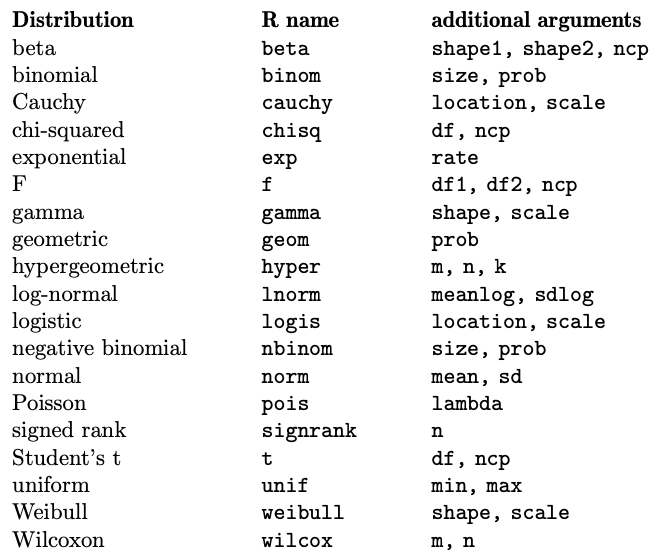
\includegraphics{img/probsR.png}

\hypertarget{distribuiuxe7uxe3o-normal}{%
\section{Distribuição Normal}\label{distribuiuxe7uxe3o-normal}}

\hypertarget{normal-univariada}{%
\subsection{Normal univariada}\label{normal-univariada}}

A distribuição normal univariada é dada pela expressão

\(f(x|\mu, \sigma) = \dfrac{1}{\sqrt{2\pi} \sigma} \exp \bigg\{ -\frac{1}{2} \left( \frac{x-\mu}{\sigma} \right) ^2 \bigg\}\)

\begin{Shaded}
\begin{Highlighting}[]
\CommentTok{\# gráfico da densidade da normal padrão, N(0,1)}
\KeywordTok{curve}\NormalTok{(}\KeywordTok{dnorm}\NormalTok{(x), }\DataTypeTok{xlim =} \KeywordTok{c}\NormalTok{(}\OperatorTok{{-}}\DecValTok{3}\NormalTok{,}\DecValTok{3}\NormalTok{))}
\end{Highlighting}
\end{Shaded}

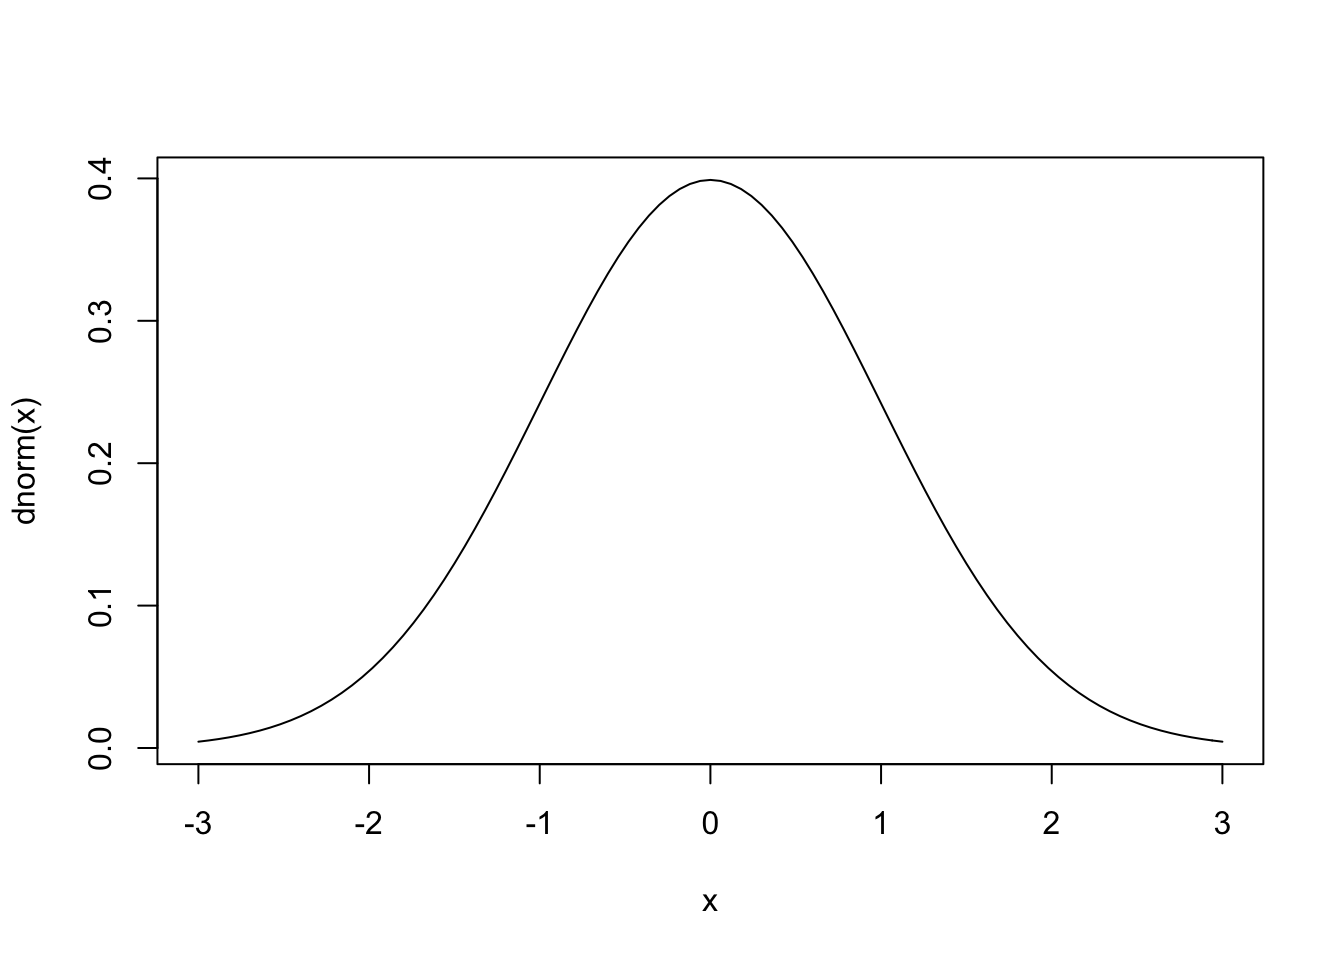
\includegraphics{_main_files/figure-latex/unnamed-chunk-39-1.pdf}

\begin{Shaded}
\begin{Highlighting}[]
\CommentTok{\# distribuição acumulada}
\KeywordTok{pnorm}\NormalTok{(}\DecValTok{0}\NormalTok{)}
\end{Highlighting}
\end{Shaded}

\begin{verbatim}
## [1] 0.5
\end{verbatim}

\begin{Shaded}
\begin{Highlighting}[]
\KeywordTok{pnorm}\NormalTok{(}\FloatTok{1.645}\NormalTok{)}
\end{Highlighting}
\end{Shaded}

\begin{verbatim}
## [1] 0.95
\end{verbatim}

\begin{Shaded}
\begin{Highlighting}[]
\KeywordTok{pnorm}\NormalTok{(}\FloatTok{1.96}\NormalTok{)}
\end{Highlighting}
\end{Shaded}

\begin{verbatim}
## [1] 0.975
\end{verbatim}

\begin{Shaded}
\begin{Highlighting}[]
\CommentTok{\# quantis (separatrizes)}
\KeywordTok{qnorm}\NormalTok{(}\FloatTok{0.5}\NormalTok{)}
\end{Highlighting}
\end{Shaded}

\begin{verbatim}
## [1] 0
\end{verbatim}

\begin{Shaded}
\begin{Highlighting}[]
\KeywordTok{qnorm}\NormalTok{(}\FloatTok{0.95}\NormalTok{)}
\end{Highlighting}
\end{Shaded}

\begin{verbatim}
## [1] 1.64
\end{verbatim}

\begin{Shaded}
\begin{Highlighting}[]
\KeywordTok{qnorm}\NormalTok{(}\FloatTok{0.975}\NormalTok{)}
\end{Highlighting}
\end{Shaded}

\begin{verbatim}
## [1] 1.96
\end{verbatim}

\hypertarget{normal-bivariada}{%
\subsection{Normal bivariada}\label{normal-bivariada}}

No caso bivariado pode-se definir

\(f(x_1,x_2|\mu_1, \mu_2, \sigma_1, \sigma_2, \rho) = \dfrac{1}{2\pi \sigma_1 \sigma_2 \sqrt{1-\rho^2}} \exp \bigg\{ -\frac{1}{2(1-\rho^2)} \left[ \frac{(x_1-\mu_1)^2}{\sigma^2_1} + \frac{(x_2-\mu_2)^2}{\sigma^2_2} - \frac{2 \rho (x_1 - \mu_1) (x_2 - \mu_2)}{\sigma_1 \sigma_2} \right] \bigg\}.\)

\begin{exercise}
\protect\hypertarget{exr:unnamed-chunk-40}{}{\label{exr:unnamed-chunk-40} }Verifique que o produto de duas normais univariadas equivale à definição no caso bivariado quando \(\rho=0\).
\end{exercise}

\begin{Shaded}
\begin{Highlighting}[]
\KeywordTok{library}\NormalTok{(rgl)}

\CommentTok{\# parâmetros}
\NormalTok{n \textless{}{-}}\StringTok{ }\DecValTok{100}
\NormalTok{x1 \textless{}{-}}\StringTok{ }\KeywordTok{seq}\NormalTok{(}\OperatorTok{{-}}\DecValTok{5}\NormalTok{, }\DecValTok{5}\NormalTok{, }\DataTypeTok{length =}\NormalTok{ n)}
\NormalTok{x2 \textless{}{-}}\StringTok{ }\KeywordTok{seq}\NormalTok{(}\OperatorTok{{-}}\DecValTok{5}\NormalTok{, }\DecValTok{5}\NormalTok{, }\DataTypeTok{length =}\NormalTok{ n)}
\NormalTok{m1 \textless{}{-}}\StringTok{ }\DecValTok{0}
\NormalTok{m2 \textless{}{-}}\StringTok{ }\DecValTok{0}
\NormalTok{s1 \textless{}{-}}\StringTok{ }\DecValTok{1}  \CommentTok{\# desvio padrão}
\NormalTok{s2 \textless{}{-}}\StringTok{ }\DecValTok{2}

\CommentTok{\# produto de normais independentes, \textbackslash{}rho = 0}
\NormalTok{z1 \textless{}{-}}\StringTok{ }\KeywordTok{outer}\NormalTok{(x1, x2, }\ControlFlowTok{function}\NormalTok{(x,y) }\KeywordTok{dnorm}\NormalTok{(x,m1,s1) }\OperatorTok{*}\StringTok{ }\KeywordTok{dnorm}\NormalTok{(y,m2,s2))}

\CommentTok{\# gráficos}
\KeywordTok{persp3d}\NormalTok{(x1, x2, z1, }\DataTypeTok{col =} \StringTok{\textquotesingle{}gray\textquotesingle{}}\NormalTok{)}
\KeywordTok{rglwidget}\NormalTok{()}
\end{Highlighting}
\end{Shaded}

\includegraphics{_main_files/figure-latex/unnamed-chunk-41-1.pdf}

\begin{Shaded}
\begin{Highlighting}[]
\KeywordTok{library}\NormalTok{(rgl)}
\KeywordTok{library}\NormalTok{(mvtnorm)}

\CommentTok{\# parâmetros}
\NormalTok{n \textless{}{-}}\StringTok{ }\DecValTok{100}
\NormalTok{x1 \textless{}{-}}\StringTok{ }\KeywordTok{seq}\NormalTok{(}\OperatorTok{{-}}\DecValTok{5}\NormalTok{, }\DecValTok{5}\NormalTok{, }\DataTypeTok{length =}\NormalTok{ n)}
\NormalTok{x2 \textless{}{-}}\StringTok{ }\KeywordTok{seq}\NormalTok{(}\OperatorTok{{-}}\DecValTok{5}\NormalTok{, }\DecValTok{5}\NormalTok{, }\DataTypeTok{length =}\NormalTok{ n)}
\NormalTok{m1 \textless{}{-}}\StringTok{ }\DecValTok{0}
\NormalTok{m2 \textless{}{-}}\StringTok{ }\DecValTok{0}
\NormalTok{s1 \textless{}{-}}\StringTok{ }\DecValTok{1}\OperatorTok{\^{}}\DecValTok{2}  \CommentTok{\# variância}
\NormalTok{s2 \textless{}{-}}\StringTok{ }\DecValTok{2}\OperatorTok{\^{}}\DecValTok{2}

\CommentTok{\# via mvtnorm::dmvnorm, \textbackslash{}rho = 0}
\NormalTok{m \textless{}{-}}\StringTok{ }\KeywordTok{c}\NormalTok{(m1,m2)}
\NormalTok{s \textless{}{-}}\StringTok{ }\KeywordTok{diag}\NormalTok{(}\KeywordTok{c}\NormalTok{(s1,s2))}
\NormalTok{z2 \textless{}{-}}\StringTok{ }\KeywordTok{outer}\NormalTok{(x1, x2, }\ControlFlowTok{function}\NormalTok{(x,y) }\KeywordTok{dmvnorm}\NormalTok{(}\KeywordTok{cbind}\NormalTok{(x,y), }\DataTypeTok{mean =}\NormalTok{ m, }\DataTypeTok{sigma =}\NormalTok{ s))}

\CommentTok{\# gráficos}
\KeywordTok{persp3d}\NormalTok{(x1, x2, z2, }\DataTypeTok{col =} \StringTok{\textquotesingle{}lightblue\textquotesingle{}}\NormalTok{)}
\KeywordTok{rglwidget}\NormalTok{()}
\end{Highlighting}
\end{Shaded}

\includegraphics{_main_files/figure-latex/unnamed-chunk-42-1.pdf}

\begin{Shaded}
\begin{Highlighting}[]
\KeywordTok{library}\NormalTok{(rgl)}
\KeywordTok{library}\NormalTok{(mvtnorm)}

\CommentTok{\# parâmetros}
\NormalTok{n \textless{}{-}}\StringTok{ }\DecValTok{100}
\NormalTok{x1 \textless{}{-}}\StringTok{ }\KeywordTok{seq}\NormalTok{(}\OperatorTok{{-}}\DecValTok{5}\NormalTok{, }\DecValTok{5}\NormalTok{, }\DataTypeTok{length =}\NormalTok{ n)}
\NormalTok{x2 \textless{}{-}}\StringTok{ }\KeywordTok{seq}\NormalTok{(}\OperatorTok{{-}}\DecValTok{5}\NormalTok{, }\DecValTok{5}\NormalTok{, }\DataTypeTok{length =}\NormalTok{ n)}
\NormalTok{m1 \textless{}{-}}\StringTok{ }\DecValTok{0}
\NormalTok{m2 \textless{}{-}}\StringTok{ }\DecValTok{0}
\NormalTok{s1 \textless{}{-}}\StringTok{ }\DecValTok{1}\OperatorTok{\^{}}\DecValTok{2}
\NormalTok{s2 \textless{}{-}}\StringTok{ }\DecValTok{2}\OperatorTok{\^{}}\DecValTok{2}
\NormalTok{r \textless{}{-}}\StringTok{ }\FloatTok{0.9}

\CommentTok{\# via mvtnorm::dmvnorm, \textbackslash{}rho = 0.9}
\NormalTok{m \textless{}{-}}\StringTok{ }\KeywordTok{c}\NormalTok{(m1,m2)}
\NormalTok{s \textless{}{-}}\StringTok{ }\KeywordTok{matrix}\NormalTok{(}\KeywordTok{c}\NormalTok{(s1,r,r,s2), }\DataTypeTok{nrow =} \DecValTok{2}\NormalTok{, }\DataTypeTok{byrow =}\NormalTok{ T)}
\NormalTok{z3 \textless{}{-}}\StringTok{ }\KeywordTok{outer}\NormalTok{(x1, x2, }\ControlFlowTok{function}\NormalTok{(x,y) }\KeywordTok{dmvnorm}\NormalTok{(}\KeywordTok{cbind}\NormalTok{(x,y), }\DataTypeTok{mean =}\NormalTok{ m, }\DataTypeTok{sigma =}\NormalTok{ s))}

\CommentTok{\# gráficos}
\KeywordTok{persp3d}\NormalTok{(x1, x2, z3, }\DataTypeTok{col =} \StringTok{\textquotesingle{}lightgreen\textquotesingle{}}\NormalTok{)}
\KeywordTok{rglwidget}\NormalTok{()}
\end{Highlighting}
\end{Shaded}

\includegraphics{_main_files/figure-latex/unnamed-chunk-43-1.pdf}

As probabilidades podem ser calculadas através da função \texttt{pmvnorm} do pacote \texttt{mvtnorm}.

\begin{Shaded}
\begin{Highlighting}[]
\KeywordTok{library}\NormalTok{(mvtnorm)}

\CommentTok{\# parâmetros}
\NormalTok{m \textless{}{-}}\StringTok{ }\KeywordTok{c}\NormalTok{(}\DecValTok{0}\NormalTok{,}\DecValTok{0}\NormalTok{)}
\NormalTok{s \textless{}{-}}\StringTok{ }\KeywordTok{diag}\NormalTok{(}\DecValTok{2}\NormalTok{)}

\CommentTok{\# Pr(X1 \textless{} 0, X2 \textless{} 0)}
\NormalTok{lower \textless{}{-}}\StringTok{ }\KeywordTok{c}\NormalTok{(}\OperatorTok{{-}}\OtherTok{Inf}\NormalTok{, }\OperatorTok{{-}}\OtherTok{Inf}\NormalTok{)}
\NormalTok{upper \textless{}{-}}\StringTok{ }\KeywordTok{c}\NormalTok{(}\DecValTok{0}\NormalTok{, }\DecValTok{0}\NormalTok{)}
\KeywordTok{pmvnorm}\NormalTok{(lower, upper, m, s)}
\end{Highlighting}
\end{Shaded}

\begin{verbatim}
## [1] 0.25
## attr(,"error")
## [1] 1e-15
## attr(,"msg")
## [1] "Normal Completion"
\end{verbatim}

\begin{exercise}
\protect\hypertarget{exr:normal-bi}{}{\label{exr:normal-bi} }Interprete o valor 0.25 calculado no exemplo acima.
\end{exercise}

\hypertarget{normal-multivariada}{%
\subsection{Normal multivariada}\label{normal-multivariada}}

Para o caso multivariado define-se

\(f(\boldsymbol{x}|\boldsymbol{\mu}, \boldsymbol{\Sigma}) = \dfrac{1}{\sqrt{2\pi} |\boldsymbol{\Sigma}|^{1/2}} \exp \bigg\{ -\frac{1}{2} (\boldsymbol{x} - \boldsymbol{\mu})' \boldsymbol{\Sigma}^{1/2} (\boldsymbol{x} - \boldsymbol{\mu}) \bigg\}\),

\(\boldsymbol{\mu} = (\mu_1,\mu_2, \ldots, \mu_p)'\), \(\boldsymbol{\Sigma} = \begin{bmatrix} \sigma_{1}^2 & \sigma_{12} & \cdots & \sigma_{1p} \\ \sigma_{12} & \sigma_{2}^2 & \cdots & \sigma_{2p} \\ \vdots & \vdots & \ddots & \vdots \\ \sigma_{1p} & \sigma_{2p} & \cdots & \sigma_{p}^2 \end{bmatrix}\).

\hypertarget{amostragem}{%
\chapter{Amostragem}\label{amostragem}}

\begin{definition}
\protect\hypertarget{def:unnamed-chunk-45}{}{\label{def:unnamed-chunk-45} }\emph{Amostragem} é o processo de obtenção de uma amostra. \(\\\)
\end{definition}
Inicia com o \emph{plano amostral}, uma avaliação que leva em conta as medidas a serem avaliadas e os recursos disponíveis. Da mesma forma que os laboratórios retiram amostras de sangue para exames de saúde, cozinheiros experimentam parte da comida para provar os temperos e fábricas realizam testes destrutivos em parte da sua produção para avaliar a qualidade do que está sendo produzido. Será feita uma breve revisão dos principais conceitos de amostragem baseada em (Bolfarine and Bussab \protect\hyperlink{ref-bolfarine2005elementos}{2005}).

\hypertarget{definiuxe7uxf5es-buxe1sicas}{%
\section{Definições básicas}\label{definiuxe7uxf5es-buxe1sicas}}

\hypertarget{unidade-elementar}{%
\subsection{Unidade Elementar}\label{unidade-elementar}}

\begin{definition}
\protect\hypertarget{def:unnamed-chunk-46}{}{\label{def:unnamed-chunk-46} }A \emph{unidade elementar}, \emph{unidade populacional} ou simplesmente \emph{elemento} é a entidade portadora das informações que pretende-se coletar. \(\\\)
\end{definition}

A unidade elementar pode ser um objeto, animal ou pessoa. Em certos casos existe mais de uma maneira de definir a unidade elementar, onde se faz necessário o entendimento dos especialistas envolvidos. A unidade elementar é uma das definições mais importantes do campo científico, pois é base de toda a construção das hipóteses de pesquisa.

\begin{example}
\protect\hypertarget{exm:unnamed-chunk-47}{}{\label{exm:unnamed-chunk-47} }(Pesquisa eleitoral I) Em uma pesquisa eleitoral, classifica-se o eleitor como unidade elementar.
\end{example}

\hypertarget{unidade-amostral}{%
\subsection{Unidade Amostral}\label{unidade-amostral}}

\begin{definition}
\protect\hypertarget{def:unnamed-chunk-48}{}{\label{def:unnamed-chunk-48} }A \emph{unidade amostral} é uma composição de uma ou mais unidades elementares. \(\\\)
\end{definition}

\begin{example}
\protect\hypertarget{exm:unnamed-chunk-49}{}{\label{exm:unnamed-chunk-49} }(Pesquisa eleitoral II) Em uma pesquisa eleitoral na rua, o eleitor é também unidade amostral. Caso as entrevistas sejam feitas de casa em casa, o domicílio passa a ser unidade amostral, i.e., um conjunto de unidades elementares (eleitores).
\end{example}

\hypertarget{sistema-de-referuxeancias}{%
\subsection{Sistema de referências}\label{sistema-de-referuxeancias}}

Em relação às informações de um estudo, deve-se fazer inicialmente uma avaliação das bases de dados já disponíveis para então proceder com a avaliação da viabilidade de um levantamento de dados mais específico. Este levantamento envolve se montar um plano amostral, contratar, treinar e manter pessoas para a coleta, criar os protocolos de resposta bem como gerar e analisar os bancos de dados. Caso decida-se realizar tal levantamento, serão necessárias listas relacionando as unidades populacionais e amostrais. Na falta de tais listas, utilizam-se \emph{sistemas de referências}, que são fontes que descrevem o universo a ser investigado. Podem ser informações razoavelmente atualizadas, como mapas, censos ou listas reunidas.

\hypertarget{universo-mathcalu}{%
\section{\texorpdfstring{Universo \(\mathcal{U}\)}{Universo \textbackslash mathcal\{U\}}}\label{universo-mathcalu}}

\begin{definition}
\protect\hypertarget{def:unnamed-chunk-50}{}{\label{def:unnamed-chunk-50} }\emph{Universo} ou \emph{população} é o conjunto de todas as unidades elementares de interesse. \(\\\)
\end{definition}
Usualmente o universo possui tamanho \(N\) elevado, até mesmo infinito, mas em alguns casos pode ser relativamente pequeno. É denotado formalmente por \[\mathcal{U} = \lbrace 1,2 \ldots, N \rbrace.\]

\begin{example}
\protect\hypertarget{exm:unnamed-chunk-51}{}{\label{exm:unnamed-chunk-51} }(Pesquisa eleitoral III) Em 2018 o universo de eleitores do município de Porto Alegre compreendia 1,100,163 eleitores\footnote{Fonte: \texttt{http://www.tse.jus.br/eleicoes/estatisticas/estatisticas-eleitorais}.}, i.e., \(N=1\,100\,163\). Formalmente \[\mathcal{U} = \lbrace 1, 2 \ldots, 1\,100\,163 \rbrace.\]
\end{example}

\begin{definition}
\protect\hypertarget{def:unnamed-chunk-52}{}{\label{def:unnamed-chunk-52} }\emph{Elemento universal}, \emph{elemento populacional} ou \emph{unidade elementar} denota um elemento \(i \in \mathcal{U}\).
\end{definition}

\begin{definition}
\protect\hypertarget{def:unnamed-chunk-53}{}{\label{def:unnamed-chunk-53} }\emph{Característica(s) de interesse} denota(m) a variável ou o conjunto de \(k\) variáveis associada(o) a cada elemento do universo, anotado por \(\boldsymbol{X} = (\boldsymbol{x}_1, \boldsymbol{x}_2, \ldots, \boldsymbol{x}_N) = \left( \begin{bmatrix} x_{11} \\ x_{12} \\ \vdots \\ x_{1k} \end{bmatrix}, \begin{bmatrix} x_{21} \\ x_{22} \\ \vdots \\ x_{2k} \end{bmatrix}, \cdots , \begin{bmatrix} x_{N1} \\ x_{N2} \\ \vdots \\ x_{Nk} \end{bmatrix} \right) = \left( \begin{array}{cccc} x_{11} & x_{21} & \cdots & x_{N1} \\ x_{12} & x_{22} & \cdots & x_{N2} \\ \vdots & \vdots & \ddots & \vdots \\ x_{1k} & x_{2k} & \cdots & x_{Nk} \end{array} \right).\) \(\\\)
\end{definition}

\begin{example}
\protect\hypertarget{exm:universo}{}{\label{exm:universo} }Considere que no universo \(\mathcal{U} = \lbrace 1,2,3 \rbrace\) de tamanho \(N=3\) o sujeito 1 seja do sexo feminino com 24 anos de idade e 1.66m de altura, o sujeito 2 do sexo masculino com idade de 32 anos e 1.81m de altura, e o sujeito 3 do sexo masculino com 49 anos com altura de 1.73m. Assim, \[\boldsymbol{X} = (\boldsymbol{x}_1,\boldsymbol{x}_2,\boldsymbol{x}_3) = \left( \begin{bmatrix} 24 \\ 1.66 \\ F \end{bmatrix}, \begin{bmatrix} 32 \\ 1.81 \\ M \end{bmatrix}, \begin{bmatrix} 49 \\ 1.73 \\ M \end{bmatrix} \right) = \left( \begin{array}{ccc} 24 & 32 & 49 \\ 1.66 & 1.81 & 1.73 \\ M & F & M \end{array} \right).\]
\end{example}

\hypertarget{paruxe2metros}{%
\subsection{Parâmetros}\label{paruxe2metros}}

\begin{definition}
\protect\hypertarget{def:unnamed-chunk-54}{}{\label{def:unnamed-chunk-54} }\emph{Parâmetro universal} ou \emph{parâmetro populacional} denota uma função ou medida que depende de todas as características de interesse. \(\\\)
\end{definition}

\begin{example}
\protect\hypertarget{exm:total-univ}{}{\label{exm:total-univ} }O parâmetro \emph{total universal} é dado por
\begin{equation} 
\tau = \sum_{i=1}^N x_i.
\label{eq:total-univ}
\end{equation}
\end{example}

\begin{example}
\protect\hypertarget{exm:media-univ}{}{\label{exm:media-univ} }O parâmetro \emph{média universal} é dado por
\begin{equation} 
\mu = \frac{1}{N} \sum_{i=1}^N x_i = \frac{\tau}{N}.
\label{eq:media-univ}
\end{equation}
\end{example}

\begin{example}
\protect\hypertarget{exm:prop-univ}{}{\label{exm:prop-univ} }Uma variável é chamada \emph{dicotômica} quando assume apenas dois possíveis valores tais como sim/não, verdadeiro/falso, ligado/desligado, etc. A característica de interesse é chamada \emph{sucesso} e a outra característica de \emph{fracasso}. Por conveniência associa-se o sucesso ao valor \(x=1\) e fracasso a \(x=0\). Desta forma simboliza-se \(\sum_{i=1}^N x_i\) como o total de sucessos observados no universo. Nesta situação o parâmetro \emph{proporção universal} é dado por
\begin{equation} 
\pi = \frac{1}{N} \sum_{i=1}^N x_i.
\label{eq:prop-univ}
\end{equation}
\end{example}

\begin{example}
\protect\hypertarget{exm:var-univ}{}{\label{exm:var-univ} }O parâmetro \emph{variância universal} é dado pelas Equações \eqref{eq:var-univ1} e \eqref{eq:var-univ2}.
\end{example}

\begin{example}
\protect\hypertarget{exm:dp-univ}{}{\label{exm:dp-univ} }O parâmetro \emph{desvio padrão universal} é a raiz quadrada da variância universal, dado pela Equação \eqref{eq:dp-univ}.
\end{example}

\begin{example}
\protect\hypertarget{exm:cov-univ}{}{\label{exm:cov-univ} }O parâmetro \emph{covariância universal} é dado por
\begin{equation} 
\sigma_{XY} = Cov[X,Y] = \frac{1}{N} \sum_{i=1}^N (x_i - \mu_X)(y_i - \mu_Y).
\label{eq:cov-univ}
\end{equation}\\
\end{example}

\begin{example}
\protect\hypertarget{exm:cor-univ}{}{\label{exm:cor-univ} }O parâmetro \emph{correlaçao universal} é dado por
\begin{equation} 
\rho_{XY} = Cor[X,Y] = \frac{\sigma_{XY}}{\sigma_X \sigma_Y}.
\label{eq:cor-univ}
\end{equation}\\
\end{example}

\begin{exercise}
\protect\hypertarget{exr:unnamed-chunk-55}{}{\label{exr:unnamed-chunk-55} }Utilizando os dados do Exemplo \ref{exm:universo}, calcule os parâmetros dos Exemplos \ref{exm:total-univ} a \ref{exm:cor-univ}. \(\\\)
\end{exercise}
\begin{exercise}
\protect\hypertarget{exr:unnamed-chunk-56}{}{\label{exr:unnamed-chunk-56} }Mostre que as Equações \eqref{eq:var-univ1} e \eqref{eq:var-univ2} são equivalentes.
\end{exercise}

\hypertarget{amostras}{%
\section{Amostras}\label{amostras}}

\begin{definition}
\protect\hypertarget{def:unnamed-chunk-57}{}{\label{def:unnamed-chunk-57} }Considere o universo \(\mathcal{U} = \lbrace 1, 2, \ldots, N \rbrace\). Uma \emph{amostra} é qualquer sequência de \(n\) unidades de \(\mathcal{U}\), formalmente denotada por \[\boldsymbol{a} = (a_1,\ldots,a_n),\] onde o \(i\)-ésimo compomente de \(\boldsymbol{a}\) é tal que \(a_i \in \mathcal{U}\). \(\\\)
\end{definition}

\begin{example}
\protect\hypertarget{exm:amostra}{}{\label{exm:amostra} }Seja \(\mathcal{U} = \lbrace 1, 2, 3 \rbrace\). Os vetores \(\boldsymbol{a}_A = (2,3)\), \(\boldsymbol{a}_B = (3,3,1)\), \(\boldsymbol{a}_C = (2)\), \(\boldsymbol{a}_D = (2,2,3,3,1)\) são possíveis amostras de \(\mathcal{U}\). \(\\\)
\end{example}

\begin{example}
\protect\hypertarget{exm:unnamed-chunk-58}{}{\label{exm:unnamed-chunk-58} }No Exemplo \ref{exm:amostra}, note os tamanhos de amostra \(n_A = n(\boldsymbol{a}_A) = 2\), \(n_B = n(\boldsymbol{a}_B) = 3\), \(n_C = n(\boldsymbol{a}_C) = 1\) e \(n_D = n(\boldsymbol{a}_D) = 5\). \(\\\)
\end{example}

\begin{definition}
\protect\hypertarget{def:unnamed-chunk-59}{}{\label{def:unnamed-chunk-59} }Seja \(\mathcal{A}(\mathcal{U})\) ou simplesmente \(\mathcal{A}\) o conjunto de todas as amostras de \(\mathcal{U}\), de qualquer tamanho, e \(\mathcal{A}_{n}(\mathcal{U})\) ou simplesmente \(\mathcal{A}_{n}\) a subclasse das as amostras de tamanho \(n\). \(\\\)
\end{definition}

\begin{example}
\protect\hypertarget{exm:subclasses}{}{\label{exm:subclasses} }Se \(\mathcal{U} = \lbrace 1, 2, 3 \rbrace\), \[\mathcal{A}(\mathcal{U}) = \lbrace (1),(2),(3),(1,1),(1,2),(1,3),(2,1),\ldots,(3,1,2,2,1),\ldots \rbrace,\]
\[\mathcal{A}_{1}(\mathcal{U}) = \lbrace (1),(2),(3) \rbrace, \] \[\mathcal{A}_{2}(\mathcal{U}) = \lbrace (1,1),(1,2),(1,3),(2,1),(2,2),(2,3),(3,1),(3,2),(3,3) \rbrace. \]
Simplificadamente \[\mathcal{A} = \lbrace 1,2,3,11,12,13,21,\ldots,31221,\ldots \rbrace,\]
\[\mathcal{A}_{1} = \lbrace 1,2,3 \rbrace, \] \[\mathcal{A}_{2} = \lbrace 11,12,13,21,22,23,31,32,33 \rbrace. \]
\end{example}

\begin{example}
\protect\hypertarget{exm:unnamed-chunk-60}{}{\label{exm:unnamed-chunk-60} }No exemplo anterior, note o número de elementos (cardinalidade) de cada conjunto: \[|\mathcal{U}|=3\]
\[|\mathcal{A}(\mathcal{U})| = \infty\]
\[|\mathcal{A}_{1}(\mathcal{U})| = 3^1 = 3\]
\[|\mathcal{A}_{2}(\mathcal{U})| = 3^2 = 9\]
\[\vdots\]
\[|\mathcal{A}_{n}(\mathcal{U})| = |\mathcal{U}|^n.\]
\end{example}

\hypertarget{plano-amostral}{%
\subsection{Plano Amostral}\label{plano-amostral}}

\begin{definition}
\protect\hypertarget{def:unnamed-chunk-61}{}{\label{def:unnamed-chunk-61} }Um \emph{plano amostral (ordenado)} é uma função \(P(\boldsymbol{a})\) definida em \(\mathcal{A}(\mathcal{U})\) satisfazendo \[P(\boldsymbol{a}) \ge 0, \; \forall \boldsymbol{a} \in \mathcal{A}(\mathcal{U}),\] tal que \[\sum_{\boldsymbol{a} \in \mathcal{A}} P(\boldsymbol{a}) =  1.\] \(\\\)
\end{definition}

\begin{example}
\protect\hypertarget{exm:planos}{}{\label{exm:planos} }Considere \(\mathcal{U} = \lbrace 1, 2, 3 \rbrace\) e \(\mathcal{A}(\mathcal{U})\) conforme Exemplo \ref{exm:subclasses}. É possivel criar infinitos planos amostrais, tais como:
\end{example}
- \textbf{Plano A \(\cdot\) Amostragem Aleatória Simples \emph{com} reposição (AASc)}
\[P(11)=P(12)=P(13)=1/9 \\ 
  P(21)=P(22)=P(23)=1/9 \\ 
  P(31)=P(32)=P(33)=1/9 \\ 
  P(\boldsymbol{a}) = 0, \; \forall \boldsymbol{a} \in \mathcal{A}(\mathcal{U}).\]

\begin{itemize}
\item
  \textbf{Plano B \(\cdot\) Amostragem Aleatória Simples \emph{sem} reposição (AASs)}
  \[P(12)=P(13)=1/6 \\
  P(21)=P(23)=1/6 \\
  P(31)=P(32)=1/6 \\
  P(\boldsymbol{a}) = 0, \; \forall \boldsymbol{a} \in \mathcal{A}(\mathcal{U}).\]
\item
  \textbf{Plano C \(\cdot\) Combinações}
  \[P(12)=P(13)=P(23)=1/3 \\
  P(\boldsymbol{a}) = 0, \; \forall \boldsymbol{a} \in \mathcal{A}(\mathcal{U}).\]
\item
  \textbf{Plano D}
  \[P(3)=9/27 \\
  P(12)=P(23)=3/27 \\
  P(111)=P(112)=P(113)=P(123)=1/27 \\
  P(221)=P(222)=P(223)=P(231)=1/27 \\
  P(331)=P(332)=P(333)=P(312)=1/27 \\
  P(\boldsymbol{a}) = 0, \; \forall \boldsymbol{a} \in \mathcal{A}(\mathcal{U}).\]
\end{itemize}

\begin{example}
\protect\hypertarget{exm:unnamed-chunk-62}{}{\label{exm:unnamed-chunk-62} }Considere a amostra \(\boldsymbol{a} = (1,2)\) obtida do universo descrito Exemplo \ref{exm:universo} a partir de algum plano amostral válido. Se o sujeito 1 tem 24 anos de idade e 1.66m de altura, e o sujeito 2 tem 32 anos de idade altura de 1.81m,
\[\boldsymbol{x} = (\boldsymbol{x}_1,\boldsymbol{x}_2) = \left( \begin{bmatrix} 24 \\ 1.66 \end{bmatrix}, \begin{bmatrix} 32 \\ 1.81 \end{bmatrix} \right) = \left( \begin{array}{cc} 24 & 32 \\ 1.66 & 1.81 \end{array} \right).\]
\end{example}

\begin{definition}
\protect\hypertarget{def:unnamed-chunk-63}{}{\label{def:unnamed-chunk-63} }Uma \emph{estatística} é uma função dos dados amostra \(\boldsymbol{a}\) anotada por \(h(\boldsymbol{x})\), i.e., qualquer medida numérica calculada a partir dos valores observados na amostra. \(\\\)
\end{definition}

\begin{example}
\protect\hypertarget{exm:estatisticas}{}{\label{exm:estatisticas} }Considere \(\boldsymbol{x}\), a matriz dos dados da amostra \(\boldsymbol{a} = (1,2)\). São exemplos de estatísticas:
\[h_1 = \frac{24+32}{2} = 28 \;\;\;\;\; \textrm{(média das idades)}\]
\[h_2 = \frac{1.66+1.81}{2} = 1.735 \;\;\;\;\; \textrm{(média das alturas)}\]
\[h_3 = 32-24 = 8 \;\;\;\;\; \textrm{(amplitude das idades)}\]
\[h_4 = \sqrt{24^2+32^2} = \sqrt{1600} = 40 \;\;\;\;\; \textrm{(norma das idades)}\]
\end{example}
\begin{exercise}
\protect\hypertarget{exr:unnamed-chunk-64}{}{\label{exr:unnamed-chunk-64} }Calcule as estatísticas do Exemplo \ref{exm:estatisticas} considerando as amostras \(\boldsymbol{a} = (1,3)\) e \(\boldsymbol{a} = (2,3)\).
\end{exercise}

\hypertarget{distribuiuxe7uxf5es-amostrais}{%
\subsection{Distribuições amostrais}\label{distribuiuxe7uxf5es-amostrais}}

\begin{definition}
\protect\hypertarget{def:unnamed-chunk-65}{}{\label{def:unnamed-chunk-65} }A \emph{distribuição amostral} de uma estatística \(h(\boldsymbol{x})\) segundo um plano amostral \(\lambda\), é a distribuição de probabilidades \(H(\boldsymbol{x})\) definida sobre \(\mathcal{A}_\lambda\), com função de probabilidade \[p_h = P_\lambda(H(\boldsymbol{x})=h) = P(h) = \frac{f_h}{|\mathcal{A}_\lambda|}. \] \(\\\)
\end{definition}

\begin{example}
\protect\hypertarget{exm:aasc}{}{\label{exm:aasc} }Considere a variável \texttt{idade} do Exemplo \ref{exm:universo} e as estatísticas \(h_1(\boldsymbol{x})=\frac{1}{n}\sum_{i=1}^n x_i\) e \(h_2(\boldsymbol{x})=\frac{1}{n-1}\sum_{i=1}^n (x_i-h_1(\boldsymbol{x}))^2\) aplicadas sobre o plano amostral A do Exemplo \ref{exm:planos}. Note que \(h_1(\boldsymbol{x})\) e \(h_2(\boldsymbol{x})\) são respectivamente a média e a variância amostrais. \(\\\)
\end{example}

\begin{itemize}
\tightlist
\item
  \textbf{Plano A \(\cdot\) Amostragem Aleatória Simples \emph{com} reposição (AASc)}
\end{itemize}

\begin{longtable}[]{@{}llllllllll@{}}
\toprule
\endhead
\begin{minipage}[t]{0.18\columnwidth}\raggedright
\(i\)\strut
\end{minipage} & \begin{minipage}[t]{0.06\columnwidth}\raggedright
1\strut
\end{minipage} & \begin{minipage}[t]{0.06\columnwidth}\raggedright
2\strut
\end{minipage} & \begin{minipage}[t]{0.06\columnwidth}\raggedright
3\strut
\end{minipage} & \begin{minipage}[t]{0.06\columnwidth}\raggedright
4\strut
\end{minipage} & \begin{minipage}[t]{0.06\columnwidth}\raggedright
5\strut
\end{minipage} & \begin{minipage}[t]{0.06\columnwidth}\raggedright
6\strut
\end{minipage} & \begin{minipage}[t]{0.06\columnwidth}\raggedright
7\strut
\end{minipage} & \begin{minipage}[t]{0.06\columnwidth}\raggedright
8\strut
\end{minipage} & \begin{minipage}[t]{0.06\columnwidth}\raggedright
9\strut
\end{minipage}\tabularnewline
\begin{minipage}[t]{0.18\columnwidth}\raggedright
\(\boldsymbol{a}\)\strut
\end{minipage} & \begin{minipage}[t]{0.06\columnwidth}\raggedright
11\strut
\end{minipage} & \begin{minipage}[t]{0.06\columnwidth}\raggedright
12\strut
\end{minipage} & \begin{minipage}[t]{0.06\columnwidth}\raggedright
13\strut
\end{minipage} & \begin{minipage}[t]{0.06\columnwidth}\raggedright
21\strut
\end{minipage} & \begin{minipage}[t]{0.06\columnwidth}\raggedright
22\strut
\end{minipage} & \begin{minipage}[t]{0.06\columnwidth}\raggedright
23\strut
\end{minipage} & \begin{minipage}[t]{0.06\columnwidth}\raggedright
31\strut
\end{minipage} & \begin{minipage}[t]{0.06\columnwidth}\raggedright
32\strut
\end{minipage} & \begin{minipage}[t]{0.06\columnwidth}\raggedright
33\strut
\end{minipage}\tabularnewline
\begin{minipage}[t]{0.18\columnwidth}\raggedright
\(P(\boldsymbol{a})\)\strut
\end{minipage} & \begin{minipage}[t]{0.06\columnwidth}\raggedright
1/9\strut
\end{minipage} & \begin{minipage}[t]{0.06\columnwidth}\raggedright
1/9\strut
\end{minipage} & \begin{minipage}[t]{0.06\columnwidth}\raggedright
1/9\strut
\end{minipage} & \begin{minipage}[t]{0.06\columnwidth}\raggedright
1/9\strut
\end{minipage} & \begin{minipage}[t]{0.06\columnwidth}\raggedright
1/9\strut
\end{minipage} & \begin{minipage}[t]{0.06\columnwidth}\raggedright
1/9\strut
\end{minipage} & \begin{minipage}[t]{0.06\columnwidth}\raggedright
1/9\strut
\end{minipage} & \begin{minipage}[t]{0.06\columnwidth}\raggedright
1/9\strut
\end{minipage} & \begin{minipage}[t]{0.06\columnwidth}\raggedright
1/9\strut
\end{minipage}\tabularnewline
\begin{minipage}[t]{0.18\columnwidth}\raggedright
\(\boldsymbol{x}\)\strut
\end{minipage} & \begin{minipage}[t]{0.06\columnwidth}\raggedright
(24,24)\strut
\end{minipage} & \begin{minipage}[t]{0.06\columnwidth}\raggedright
(24,32)\strut
\end{minipage} & \begin{minipage}[t]{0.06\columnwidth}\raggedright
(24,49)\strut
\end{minipage} & \begin{minipage}[t]{0.06\columnwidth}\raggedright
(32,24)\strut
\end{minipage} & \begin{minipage}[t]{0.06\columnwidth}\raggedright
(32,32)\strut
\end{minipage} & \begin{minipage}[t]{0.06\columnwidth}\raggedright
(32,49)\strut
\end{minipage} & \begin{minipage}[t]{0.06\columnwidth}\raggedright
(49,24)\strut
\end{minipage} & \begin{minipage}[t]{0.06\columnwidth}\raggedright
(49,32)\strut
\end{minipage} & \begin{minipage}[t]{0.06\columnwidth}\raggedright
(49,49)\strut
\end{minipage}\tabularnewline
\begin{minipage}[t]{0.18\columnwidth}\raggedright
\(h_1(\boldsymbol{x})\)\strut
\end{minipage} & \begin{minipage}[t]{0.06\columnwidth}\raggedright
24.0\strut
\end{minipage} & \begin{minipage}[t]{0.06\columnwidth}\raggedright
28.0\strut
\end{minipage} & \begin{minipage}[t]{0.06\columnwidth}\raggedright
36.5\strut
\end{minipage} & \begin{minipage}[t]{0.06\columnwidth}\raggedright
28.0\strut
\end{minipage} & \begin{minipage}[t]{0.06\columnwidth}\raggedright
32.0\strut
\end{minipage} & \begin{minipage}[t]{0.06\columnwidth}\raggedright
40.5\strut
\end{minipage} & \begin{minipage}[t]{0.06\columnwidth}\raggedright
36.5\strut
\end{minipage} & \begin{minipage}[t]{0.06\columnwidth}\raggedright
40.5\strut
\end{minipage} & \begin{minipage}[t]{0.06\columnwidth}\raggedright
49.0\strut
\end{minipage}\tabularnewline
\begin{minipage}[t]{0.18\columnwidth}\raggedright
\(h_2(\boldsymbol{x})\)\strut
\end{minipage} & \begin{minipage}[t]{0.06\columnwidth}\raggedright
0.0\strut
\end{minipage} & \begin{minipage}[t]{0.06\columnwidth}\raggedright
32.0\strut
\end{minipage} & \begin{minipage}[t]{0.06\columnwidth}\raggedright
312.5\strut
\end{minipage} & \begin{minipage}[t]{0.06\columnwidth}\raggedright
32.0\strut
\end{minipage} & \begin{minipage}[t]{0.06\columnwidth}\raggedright
0.0\strut
\end{minipage} & \begin{minipage}[t]{0.06\columnwidth}\raggedright
144.5\strut
\end{minipage} & \begin{minipage}[t]{0.06\columnwidth}\raggedright
312.5\strut
\end{minipage} & \begin{minipage}[t]{0.06\columnwidth}\raggedright
144.5\strut
\end{minipage} & \begin{minipage}[t]{0.06\columnwidth}\raggedright
0.0\strut
\end{minipage}\tabularnewline
\bottomrule
\end{longtable}

\begin{longtable}[]{@{}llllllll@{}}
\toprule
\endhead
\begin{minipage}[t]{0.12\columnwidth}\raggedright
\(h_1\)\strut
\end{minipage} & \begin{minipage}[t]{0.08\columnwidth}\raggedright
24.0\strut
\end{minipage} & \begin{minipage}[t]{0.08\columnwidth}\raggedright
28.0\strut
\end{minipage} & \begin{minipage}[t]{0.08\columnwidth}\raggedright
32.0\strut
\end{minipage} & \begin{minipage}[t]{0.08\columnwidth}\raggedright
36.5\strut
\end{minipage} & \begin{minipage}[t]{0.08\columnwidth}\raggedright
40.5\strut
\end{minipage} & \begin{minipage}[t]{0.08\columnwidth}\raggedright
49.0\strut
\end{minipage} & \begin{minipage}[t]{0.11\columnwidth}\raggedright
\textbf{Total}\strut
\end{minipage}\tabularnewline
\begin{minipage}[t]{0.12\columnwidth}\raggedright
\(f_{h1}\)\strut
\end{minipage} & \begin{minipage}[t]{0.08\columnwidth}\raggedright
1\strut
\end{minipage} & \begin{minipage}[t]{0.08\columnwidth}\raggedright
2\strut
\end{minipage} & \begin{minipage}[t]{0.08\columnwidth}\raggedright
1\strut
\end{minipage} & \begin{minipage}[t]{0.08\columnwidth}\raggedright
2\strut
\end{minipage} & \begin{minipage}[t]{0.08\columnwidth}\raggedright
2\strut
\end{minipage} & \begin{minipage}[t]{0.08\columnwidth}\raggedright
1\strut
\end{minipage} & \begin{minipage}[t]{0.11\columnwidth}\raggedright
\textbf{9}\strut
\end{minipage}\tabularnewline
\begin{minipage}[t]{0.12\columnwidth}\raggedright
\(p_{h1}\)\strut
\end{minipage} & \begin{minipage}[t]{0.08\columnwidth}\raggedright
1/9\strut
\end{minipage} & \begin{minipage}[t]{0.08\columnwidth}\raggedright
2/9\strut
\end{minipage} & \begin{minipage}[t]{0.08\columnwidth}\raggedright
1/9\strut
\end{minipage} & \begin{minipage}[t]{0.08\columnwidth}\raggedright
2/9\strut
\end{minipage} & \begin{minipage}[t]{0.08\columnwidth}\raggedright
2/9\strut
\end{minipage} & \begin{minipage}[t]{0.08\columnwidth}\raggedright
1/9\strut
\end{minipage} & \begin{minipage}[t]{0.11\columnwidth}\raggedright
\textbf{1}\strut
\end{minipage}\tabularnewline
\bottomrule
\end{longtable}

\begin{longtable}[]{@{}llllll@{}}
\toprule
\endhead
\begin{minipage}[t]{0.13\columnwidth}\raggedright
\(h_2\)\strut
\end{minipage} & \begin{minipage}[t]{0.08\columnwidth}\raggedright
0.0\strut
\end{minipage} & \begin{minipage}[t]{0.08\columnwidth}\raggedright
32.0\strut
\end{minipage} & \begin{minipage}[t]{0.08\columnwidth}\raggedright
144.5\strut
\end{minipage} & \begin{minipage}[t]{0.08\columnwidth}\raggedright
312.5\strut
\end{minipage} & \begin{minipage}[t]{0.12\columnwidth}\raggedright
\textbf{Total}\strut
\end{minipage}\tabularnewline
\begin{minipage}[t]{0.13\columnwidth}\raggedright
\(f_{h2}\)\strut
\end{minipage} & \begin{minipage}[t]{0.08\columnwidth}\raggedright
3\strut
\end{minipage} & \begin{minipage}[t]{0.08\columnwidth}\raggedright
2\strut
\end{minipage} & \begin{minipage}[t]{0.08\columnwidth}\raggedright
2\strut
\end{minipage} & \begin{minipage}[t]{0.08\columnwidth}\raggedright
2\strut
\end{minipage} & \begin{minipage}[t]{0.12\columnwidth}\raggedright
\textbf{9}\strut
\end{minipage}\tabularnewline
\begin{minipage}[t]{0.13\columnwidth}\raggedright
\(p_{h2}\)\strut
\end{minipage} & \begin{minipage}[t]{0.08\columnwidth}\raggedright
3/9\strut
\end{minipage} & \begin{minipage}[t]{0.08\columnwidth}\raggedright
2/9\strut
\end{minipage} & \begin{minipage}[t]{0.08\columnwidth}\raggedright
2/9\strut
\end{minipage} & \begin{minipage}[t]{0.08\columnwidth}\raggedright
2/9\strut
\end{minipage} & \begin{minipage}[t]{0.12\columnwidth}\raggedright
\textbf{1}\strut
\end{minipage}\tabularnewline
\bottomrule
\end{longtable}

\(\\\)
\begin{example}
\protect\hypertarget{exm:aass}{}{\label{exm:aass} }Considere novamente a variável \texttt{idade} do Exemplo \ref{exm:universo} e a estatística \(h_1(\boldsymbol{x})=\frac{1}{n}\sum_{i=1}^n x_i\), agora aplicada sobre o plano amostral B do Exemplo \ref{exm:planos}. \(\\\)
\end{example}

\begin{itemize}
\tightlist
\item
  \textbf{Plano B \(\cdot\) Amostragem Aleatória Simples \emph{sem} reposição (AASs)}
\end{itemize}

\begin{longtable}[]{@{}lllllll@{}}
\toprule
\endhead
\begin{minipage}[t]{0.27\columnwidth}\raggedright
\(i\)\strut
\end{minipage} & \begin{minipage}[t]{0.09\columnwidth}\raggedright
1\strut
\end{minipage} & \begin{minipage}[t]{0.09\columnwidth}\raggedright
2\strut
\end{minipage} & \begin{minipage}[t]{0.09\columnwidth}\raggedright
3\strut
\end{minipage} & \begin{minipage}[t]{0.09\columnwidth}\raggedright
4\strut
\end{minipage} & \begin{minipage}[t]{0.09\columnwidth}\raggedright
5\strut
\end{minipage} & \begin{minipage}[t]{0.09\columnwidth}\raggedright
6\strut
\end{minipage}\tabularnewline
\begin{minipage}[t]{0.27\columnwidth}\raggedright
\(\boldsymbol{a}\)\strut
\end{minipage} & \begin{minipage}[t]{0.09\columnwidth}\raggedright
12\strut
\end{minipage} & \begin{minipage}[t]{0.09\columnwidth}\raggedright
13\strut
\end{minipage} & \begin{minipage}[t]{0.09\columnwidth}\raggedright
21\strut
\end{minipage} & \begin{minipage}[t]{0.09\columnwidth}\raggedright
23\strut
\end{minipage} & \begin{minipage}[t]{0.09\columnwidth}\raggedright
31\strut
\end{minipage} & \begin{minipage}[t]{0.09\columnwidth}\raggedright
32\strut
\end{minipage}\tabularnewline
\begin{minipage}[t]{0.27\columnwidth}\raggedright
\(P(\boldsymbol{a})\)\strut
\end{minipage} & \begin{minipage}[t]{0.09\columnwidth}\raggedright
1/6\strut
\end{minipage} & \begin{minipage}[t]{0.09\columnwidth}\raggedright
1/6\strut
\end{minipage} & \begin{minipage}[t]{0.09\columnwidth}\raggedright
1/6\strut
\end{minipage} & \begin{minipage}[t]{0.09\columnwidth}\raggedright
1/6\strut
\end{minipage} & \begin{minipage}[t]{0.09\columnwidth}\raggedright
1/6\strut
\end{minipage} & \begin{minipage}[t]{0.09\columnwidth}\raggedright
1/6\strut
\end{minipage}\tabularnewline
\begin{minipage}[t]{0.27\columnwidth}\raggedright
\(\boldsymbol{x}\)\strut
\end{minipage} & \begin{minipage}[t]{0.09\columnwidth}\raggedright
(24,32)\strut
\end{minipage} & \begin{minipage}[t]{0.09\columnwidth}\raggedright
(24,49)\strut
\end{minipage} & \begin{minipage}[t]{0.09\columnwidth}\raggedright
(32,24)\strut
\end{minipage} & \begin{minipage}[t]{0.09\columnwidth}\raggedright
(32,49)\strut
\end{minipage} & \begin{minipage}[t]{0.09\columnwidth}\raggedright
(49,24)\strut
\end{minipage} & \begin{minipage}[t]{0.09\columnwidth}\raggedright
(49,32)\strut
\end{minipage}\tabularnewline
\begin{minipage}[t]{0.27\columnwidth}\raggedright
\(h_1(\boldsymbol{x})\)\strut
\end{minipage} & \begin{minipage}[t]{0.09\columnwidth}\raggedright
28.0\strut
\end{minipage} & \begin{minipage}[t]{0.09\columnwidth}\raggedright
36.5\strut
\end{minipage} & \begin{minipage}[t]{0.09\columnwidth}\raggedright
28.0\strut
\end{minipage} & \begin{minipage}[t]{0.09\columnwidth}\raggedright
40.5\strut
\end{minipage} & \begin{minipage}[t]{0.09\columnwidth}\raggedright
36.5\strut
\end{minipage} & \begin{minipage}[t]{0.09\columnwidth}\raggedright
40.5\strut
\end{minipage}\tabularnewline
\bottomrule
\end{longtable}

\begin{longtable}[]{@{}lllll@{}}
\toprule
\endhead
\begin{minipage}[t]{0.13\columnwidth}\raggedright
\(h_1\)\strut
\end{minipage} & \begin{minipage}[t]{0.08\columnwidth}\raggedright
28.0\strut
\end{minipage} & \begin{minipage}[t]{0.08\columnwidth}\raggedright
36.5\strut
\end{minipage} & \begin{minipage}[t]{0.08\columnwidth}\raggedright
40.5\strut
\end{minipage} & \begin{minipage}[t]{0.12\columnwidth}\raggedright
\textbf{Total}\strut
\end{minipage}\tabularnewline
\begin{minipage}[t]{0.13\columnwidth}\raggedright
\(f_{h1}\)\strut
\end{minipage} & \begin{minipage}[t]{0.08\columnwidth}\raggedright
2\strut
\end{minipage} & \begin{minipage}[t]{0.08\columnwidth}\raggedright
2\strut
\end{minipage} & \begin{minipage}[t]{0.08\columnwidth}\raggedright
2\strut
\end{minipage} & \begin{minipage}[t]{0.12\columnwidth}\raggedright
\textbf{6}\strut
\end{minipage}\tabularnewline
\begin{minipage}[t]{0.13\columnwidth}\raggedright
\(p_{h1}\)\strut
\end{minipage} & \begin{minipage}[t]{0.08\columnwidth}\raggedright
2/6\strut
\end{minipage} & \begin{minipage}[t]{0.08\columnwidth}\raggedright
2/6\strut
\end{minipage} & \begin{minipage}[t]{0.08\columnwidth}\raggedright
2/6\strut
\end{minipage} & \begin{minipage}[t]{0.12\columnwidth}\raggedright
\textbf{1}\strut
\end{minipage}\tabularnewline
\bottomrule
\end{longtable}

\(\\\)
\begin{example}
\protect\hypertarget{exm:comb}{}{\label{exm:comb} }Considere novamente a variável \texttt{idade} do Exemplo \ref{exm:universo} e a estatística \(h_1(\boldsymbol{x})=\frac{1}{n}\sum_{i=1}^n x_i\), agora aplicada sobre o plano amostral C do Exemplo \ref{exm:planos}. \(\\\)
\end{example}
- \textbf{Plano C \(\cdot\) Combinações}

\begin{longtable}[]{@{}llll@{}}
\toprule
\endhead
\begin{minipage}[t]{0.30\columnwidth}\raggedright
\(i\)\strut
\end{minipage} & \begin{minipage}[t]{0.10\columnwidth}\raggedright
1\strut
\end{minipage} & \begin{minipage}[t]{0.10\columnwidth}\raggedright
2\strut
\end{minipage} & \begin{minipage}[t]{0.10\columnwidth}\raggedright
3\strut
\end{minipage}\tabularnewline
\begin{minipage}[t]{0.30\columnwidth}\raggedright
\(\boldsymbol{a}\)\strut
\end{minipage} & \begin{minipage}[t]{0.10\columnwidth}\raggedright
12\strut
\end{minipage} & \begin{minipage}[t]{0.10\columnwidth}\raggedright
13\strut
\end{minipage} & \begin{minipage}[t]{0.10\columnwidth}\raggedright
23\strut
\end{minipage}\tabularnewline
\begin{minipage}[t]{0.30\columnwidth}\raggedright
\(P(\boldsymbol{a})\)\strut
\end{minipage} & \begin{minipage}[t]{0.10\columnwidth}\raggedright
1/3\strut
\end{minipage} & \begin{minipage}[t]{0.10\columnwidth}\raggedright
1/3\strut
\end{minipage} & \begin{minipage}[t]{0.10\columnwidth}\raggedright
1/3\strut
\end{minipage}\tabularnewline
\begin{minipage}[t]{0.30\columnwidth}\raggedright
\(\boldsymbol{x}\)\strut
\end{minipage} & \begin{minipage}[t]{0.10\columnwidth}\raggedright
(24,32)\strut
\end{minipage} & \begin{minipage}[t]{0.10\columnwidth}\raggedright
(24,49)\strut
\end{minipage} & \begin{minipage}[t]{0.10\columnwidth}\raggedright
(32,49)\strut
\end{minipage}\tabularnewline
\begin{minipage}[t]{0.30\columnwidth}\raggedright
\(h_1(\boldsymbol{x})\)\strut
\end{minipage} & \begin{minipage}[t]{0.10\columnwidth}\raggedright
28.0\strut
\end{minipage} & \begin{minipage}[t]{0.10\columnwidth}\raggedright
36.5\strut
\end{minipage} & \begin{minipage}[t]{0.10\columnwidth}\raggedright
40.5\strut
\end{minipage}\tabularnewline
\bottomrule
\end{longtable}

\begin{longtable}[]{@{}lllll@{}}
\toprule
\endhead
\begin{minipage}[t]{0.13\columnwidth}\raggedright
\(h_1\)\strut
\end{minipage} & \begin{minipage}[t]{0.08\columnwidth}\raggedright
28.0\strut
\end{minipage} & \begin{minipage}[t]{0.08\columnwidth}\raggedright
36.5\strut
\end{minipage} & \begin{minipage}[t]{0.08\columnwidth}\raggedright
40.5\strut
\end{minipage} & \begin{minipage}[t]{0.12\columnwidth}\raggedright
\textbf{Total}\strut
\end{minipage}\tabularnewline
\begin{minipage}[t]{0.13\columnwidth}\raggedright
\(f_{h1}\)\strut
\end{minipage} & \begin{minipage}[t]{0.08\columnwidth}\raggedright
1\strut
\end{minipage} & \begin{minipage}[t]{0.08\columnwidth}\raggedright
1\strut
\end{minipage} & \begin{minipage}[t]{0.08\columnwidth}\raggedright
1\strut
\end{minipage} & \begin{minipage}[t]{0.12\columnwidth}\raggedright
\textbf{3}\strut
\end{minipage}\tabularnewline
\begin{minipage}[t]{0.13\columnwidth}\raggedright
\(p_{h1}\)\strut
\end{minipage} & \begin{minipage}[t]{0.08\columnwidth}\raggedright
1/3\strut
\end{minipage} & \begin{minipage}[t]{0.08\columnwidth}\raggedright
1/3\strut
\end{minipage} & \begin{minipage}[t]{0.08\columnwidth}\raggedright
1/3\strut
\end{minipage} & \begin{minipage}[t]{0.12\columnwidth}\raggedright
\textbf{1}\strut
\end{minipage}\tabularnewline
\bottomrule
\end{longtable}

\(\\\)
\begin{exercise}
\protect\hypertarget{exr:unnamed-chunk-66}{}{\label{exr:unnamed-chunk-66} }Refaça os Exemplos \ref{exm:aasc}, \ref{exm:aass} e \ref{exm:comb} considerando a variável \texttt{altura}. Para os Exemplos \ref{exm:aass} e \ref{exm:comb}, calcule também a estatística \(h_2(\boldsymbol{x})=\frac{1}{n-1}\sum_{i=1}^n (x_i-h_1(\boldsymbol{x}))^2\). \(\\\)
\end{exercise}

\begin{example}
\protect\hypertarget{exm:aas-R}{}{\label{exm:aas-R} }A seguir são implementadas em R as resoluções dos Exemplos \ref{exm:aasc} e \ref{exm:aass}.
\end{example}

\begin{Shaded}
\begin{Highlighting}[]
\NormalTok{U \textless{}{-}}\StringTok{ }\DecValTok{1}\OperatorTok{:}\DecValTok{3}                    \CommentTok{\# universo}
\NormalTok{(aasc \textless{}{-}}\StringTok{ }\KeywordTok{expand.grid}\NormalTok{(U,U))  }\CommentTok{\# AASc de tamanho n=2}
\end{Highlighting}
\end{Shaded}

\begin{verbatim}
##   Var1 Var2
## 1    1    1
## 2    2    1
## 3    3    1
## 4    1    2
## 5    2    2
## 6    3    2
## 7    1    3
## 8    2    3
## 9    3    3
\end{verbatim}

\begin{Shaded}
\begin{Highlighting}[]
\NormalTok{(aasc \textless{}{-}}\StringTok{ }\KeywordTok{cbind}\NormalTok{(aasc[,}\DecValTok{2}\NormalTok{],aasc[,}\DecValTok{1}\NormalTok{])) }\CommentTok{\# trocando as colunas para melhor leitura}
\end{Highlighting}
\end{Shaded}

\begin{verbatim}
##       [,1] [,2]
##  [1,]    1    1
##  [2,]    1    2
##  [3,]    1    3
##  [4,]    2    1
##  [5,]    2    2
##  [6,]    2    3
##  [7,]    3    1
##  [8,]    3    2
##  [9,]    3    3
\end{verbatim}

\begin{Shaded}
\begin{Highlighting}[]
\NormalTok{(aass \textless{}{-}}\StringTok{ }\NormalTok{aasc[}\OperatorTok{{-}}\KeywordTok{c}\NormalTok{(}\DecValTok{1}\NormalTok{,}\DecValTok{5}\NormalTok{,}\DecValTok{9}\NormalTok{),]) }\CommentTok{\# AASs de tamanho n=2}
\end{Highlighting}
\end{Shaded}

\begin{verbatim}
##      [,1] [,2]
## [1,]    1    2
## [2,]    1    3
## [3,]    2    1
## [4,]    2    3
## [5,]    3    1
## [6,]    3    2
\end{verbatim}

\begin{Shaded}
\begin{Highlighting}[]
\NormalTok{x1 \textless{}{-}}\StringTok{ }\KeywordTok{c}\NormalTok{(}\DecValTok{24}\NormalTok{,}\DecValTok{32}\NormalTok{,}\DecValTok{49}\NormalTok{)           }\CommentTok{\# dados de idade}
\NormalTok{n \textless{}{-}}\StringTok{ }\KeywordTok{ncol}\NormalTok{(aasc)}
\CommentTok{\# AASc}
\NormalTok{(xc \textless{}{-}}\StringTok{ }\KeywordTok{cbind}\NormalTok{(x1[aasc[,}\DecValTok{1}\NormalTok{]], x1[aasc[,}\DecValTok{2}\NormalTok{]])) }\CommentTok{\# dados amostrais de idade com reposição}
\end{Highlighting}
\end{Shaded}

\begin{verbatim}
##       [,1] [,2]
##  [1,]   24   24
##  [2,]   24   32
##  [3,]   24   49
##  [4,]   32   24
##  [5,]   32   32
##  [6,]   32   49
##  [7,]   49   24
##  [8,]   49   32
##  [9,]   49   49
\end{verbatim}

\begin{Shaded}
\begin{Highlighting}[]
\NormalTok{(mxc \textless{}{-}}\StringTok{ }\KeywordTok{rowMeans}\NormalTok{(xc))       }\CommentTok{\# estatística h1(x) aplicada na AASc}
\end{Highlighting}
\end{Shaded}

\begin{verbatim}
## [1] 24.0 28.0 36.5 28.0 32.0 40.5 36.5 40.5 49.0
\end{verbatim}

\begin{Shaded}
\begin{Highlighting}[]
\NormalTok{(tabc \textless{}{-}}\StringTok{ }\KeywordTok{table}\NormalTok{(mxc))        }\CommentTok{\# frequência amostral de h1(y) aplicada na AASc}
\end{Highlighting}
\end{Shaded}

\begin{verbatim}
## mxc
##   24   28   32 36.5 40.5   49 
##    1    2    1    2    2    1
\end{verbatim}

\begin{Shaded}
\begin{Highlighting}[]
\NormalTok{MASS}\OperatorTok{::}\KeywordTok{fractions}\NormalTok{(}\KeywordTok{prop.table}\NormalTok{(tabc)) }\CommentTok{\# distribuição amostral de h1(x) aplicada na AASc}
\end{Highlighting}
\end{Shaded}

\begin{verbatim}
## mxc
##   24   28   32 36.5 40.5   49 
##  1/9  2/9  1/9  2/9  2/9  1/9
\end{verbatim}

\begin{Shaded}
\begin{Highlighting}[]
\CommentTok{\# vyc \textless{}{-} (rowMeans(xc\^{}2){-}mxc\^{}2)*(n/(n{-}1))}
\CommentTok{\# AASs}
\NormalTok{(xs \textless{}{-}}\StringTok{ }\KeywordTok{cbind}\NormalTok{(x1[aass[,}\DecValTok{1}\NormalTok{]], x1[aass[,}\DecValTok{2}\NormalTok{]])) }\CommentTok{\# dados amostrais de idade sem reposição}
\end{Highlighting}
\end{Shaded}

\begin{verbatim}
##      [,1] [,2]
## [1,]   24   32
## [2,]   24   49
## [3,]   32   24
## [4,]   32   49
## [5,]   49   24
## [6,]   49   32
\end{verbatim}

\begin{Shaded}
\begin{Highlighting}[]
\NormalTok{(mxs \textless{}{-}}\StringTok{ }\KeywordTok{rowMeans}\NormalTok{(xs))       }\CommentTok{\# estatística h(x) aplicada na AASs}
\end{Highlighting}
\end{Shaded}

\begin{verbatim}
## [1] 28.0 36.5 28.0 40.5 36.5 40.5
\end{verbatim}

\begin{Shaded}
\begin{Highlighting}[]
\NormalTok{(tabs \textless{}{-}}\StringTok{ }\KeywordTok{table}\NormalTok{(mxs))        }\CommentTok{\# frequência amostral de h(x) aplicada na AASs}
\end{Highlighting}
\end{Shaded}

\begin{verbatim}
## mxs
##   28 36.5 40.5 
##    2    2    2
\end{verbatim}

\begin{Shaded}
\begin{Highlighting}[]
\NormalTok{MASS}\OperatorTok{::}\KeywordTok{fractions}\NormalTok{(}\KeywordTok{prop.table}\NormalTok{(tabs)) }\CommentTok{\# distribuição amostral de h(x) aplicada na AASs}
\end{Highlighting}
\end{Shaded}

\begin{verbatim}
## mxs
##   28 36.5 40.5 
##  1/3  1/3  1/3
\end{verbatim}

\begin{example}
\protect\hypertarget{exm:aas-R-arr}{}{\label{exm:aas-R-arr} }As resoluçãos dos Exemplos \ref{exm:aass} e \ref{exm:comb} podem ser implementadas no pacote \href{https://cran.r-project.org/web/packages/arrangements/}{\texttt{arrangements}} do R. Note que são obtidas as amostras via AASs através da função \texttt{permutations} e as amostras por combinação, sem qualquer tipo de repetição, pela função \texttt{combinations}.
\end{example}

\begin{Shaded}
\begin{Highlighting}[]
\KeywordTok{library}\NormalTok{(arrangements)}
\NormalTok{x1 \textless{}{-}}\StringTok{ }\KeywordTok{c}\NormalTok{(}\DecValTok{24}\NormalTok{,}\DecValTok{32}\NormalTok{,}\DecValTok{49}\NormalTok{)  }\CommentTok{\# dados de idade}
\CommentTok{\# AASs}
\KeywordTok{npermutations}\NormalTok{(}\DecValTok{3}\NormalTok{,}\DecValTok{2}\NormalTok{) }\CommentTok{\# número de AASs}
\end{Highlighting}
\end{Shaded}

\begin{verbatim}
## [1] 6
\end{verbatim}

\begin{Shaded}
\begin{Highlighting}[]
\NormalTok{(aass \textless{}{-}}\StringTok{ }\KeywordTok{permutations}\NormalTok{(}\DecValTok{3}\NormalTok{,}\DecValTok{2}\NormalTok{)) }\CommentTok{\# gerando as AASs}
\end{Highlighting}
\end{Shaded}

\begin{verbatim}
##      [,1] [,2]
## [1,]    1    2
## [2,]    1    3
## [3,]    2    1
## [4,]    2    3
## [5,]    3    1
## [6,]    3    2
\end{verbatim}

\begin{Shaded}
\begin{Highlighting}[]
\NormalTok{(maass \textless{}{-}}\StringTok{ }\KeywordTok{matrix}\NormalTok{(x1[}\KeywordTok{t}\NormalTok{(aass)], }\DataTypeTok{ncol=}\DecValTok{2}\NormalTok{, }\DataTypeTok{byrow =}\NormalTok{ T))}
\end{Highlighting}
\end{Shaded}

\begin{verbatim}
##      [,1] [,2]
## [1,]   24   32
## [2,]   24   49
## [3,]   32   24
## [4,]   32   49
## [5,]   49   24
## [6,]   49   32
\end{verbatim}

\begin{Shaded}
\begin{Highlighting}[]
\KeywordTok{rowMeans}\NormalTok{(maass)}
\end{Highlighting}
\end{Shaded}

\begin{verbatim}
## [1] 28.0 36.5 28.0 40.5 36.5 40.5
\end{verbatim}

\begin{Shaded}
\begin{Highlighting}[]
\KeywordTok{mean}\NormalTok{(}\KeywordTok{rowMeans}\NormalTok{(maass)) }\CommentTok{\# plano amostral não viesado}
\end{Highlighting}
\end{Shaded}

\begin{verbatim}
## [1] 35
\end{verbatim}

\begin{Shaded}
\begin{Highlighting}[]
\CommentTok{\# Combinações}
\KeywordTok{ncombinations}\NormalTok{(}\DecValTok{3}\NormalTok{,}\DecValTok{2}\NormalTok{) }\CommentTok{\# número de amostras via combinação}
\end{Highlighting}
\end{Shaded}

\begin{verbatim}
## [1] 3
\end{verbatim}

\begin{Shaded}
\begin{Highlighting}[]
\NormalTok{(comb \textless{}{-}}\StringTok{ }\KeywordTok{combinations}\NormalTok{(}\DecValTok{3}\NormalTok{,}\DecValTok{2}\NormalTok{)) }\CommentTok{\# gerando as amostras via combinação}
\end{Highlighting}
\end{Shaded}

\begin{verbatim}
##      [,1] [,2]
## [1,]    1    2
## [2,]    1    3
## [3,]    2    3
\end{verbatim}

\begin{Shaded}
\begin{Highlighting}[]
\NormalTok{(mcomb \textless{}{-}}\StringTok{ }\KeywordTok{matrix}\NormalTok{(x1[}\KeywordTok{t}\NormalTok{(comb)], }\DataTypeTok{ncol=}\DecValTok{2}\NormalTok{, }\DataTypeTok{byrow =}\NormalTok{ T))}
\end{Highlighting}
\end{Shaded}

\begin{verbatim}
##      [,1] [,2]
## [1,]   24   32
## [2,]   24   49
## [3,]   32   49
\end{verbatim}

\begin{Shaded}
\begin{Highlighting}[]
\KeywordTok{rowMeans}\NormalTok{(mcomb)}
\end{Highlighting}
\end{Shaded}

\begin{verbatim}
## [1] 28.0 36.5 40.5
\end{verbatim}

\begin{Shaded}
\begin{Highlighting}[]
\KeywordTok{mean}\NormalTok{(}\KeywordTok{rowMeans}\NormalTok{(mcomb)) }\CommentTok{\# plano amostral não viesado}
\end{Highlighting}
\end{Shaded}

\begin{verbatim}
## [1] 35
\end{verbatim}

\begin{conjecture}
\protect\hypertarget{cnj:unnamed-chunk-69}{}{\label{cnj:unnamed-chunk-69} }Generalize os Exemplos \ref{exm:aas-R} e \ref{exm:comb} para qualquer tamanho de amostra, parametrizando as opções com e sem reposição, bem como para combinações. Por fim, adicione um argumento que permita calcular qualquer estatística.
\end{conjecture}

\hypertarget{teorema-central-do-limite}{%
\subsubsection*{Teorema Central do Limite}\label{teorema-central-do-limite}}
\addcontentsline{toc}{subsubsection}{Teorema Central do Limite}

O \emph{Teorema Central do Limite} (TCL) é um dos principais resultados da Probabilidade. Ele mostra que, sob certas condições razoavelmente alcançadas na prática, a soma ou média de uma sequência de variáveis aleatórias independentes e identicamente distribuídas (\emph{iid})\footnote{Variáveis que apresentam mesma distribuição de probabilidade com os mesmos parâmetros.} têm distribuição aproximadamente normal. Este resultado permite a resolução aproximada de problemas que envolvam muitos cálculos, usualmente impraticáveis dado o volume de operações necessárias.

\begin{theorem}
\protect\hypertarget{thm:tcl}{}{\label{thm:tcl} }(Teorema Central do Limite de Lindeberg-Lévy) Seja \(X_{1}, X_{2}, \ldots, X_{n}\) uma sequência de variáveis aleatórias iid com \(E(X_{i}) = \mu\) e \(V(X_{i}) = \sigma^2\). Considerando \(S=X_{1}+X_{2}+\ldots+X_{n}\), \(M=S/n\) e se \(n \longrightarrow \infty\), então
\begin{equation}
Z = \frac{S - n\mu}{\sigma \sqrt{n}} = \dfrac{M - \mu}{\sigma / \sqrt{n}} \xrightarrow{D} \mathcal{N}(0,1).
\label{eq:tcl}
\end{equation}
\end{theorem}

A \emph{correção de continuidade} ocorre quando soma-se 0.5 no numerador da Equação \eqref{eq:tcl}. (James \protect\hyperlink{ref-james2010probabilidade}{2010}) sugere o uso da expressão `Teorema Central do Limite' no lugar de `Teorema do Limite Central', pois central é o teorema, não o limite. A origem da expressão é atribuída ao matemático húngaro George Pólya, ao se referir a \emph{der zentrale Grenzwertsatz}, i.e., o `central' refere-se ao `teorema do limite'.

\hypertarget{distribuiuxe7uxe3o-amostral-da-proporuxe7uxe3o}{%
\subsubsection*{Distribuição amostral da proporção}\label{distribuiuxe7uxe3o-amostral-da-proporuxe7uxe3o}}
\addcontentsline{toc}{subsubsection}{Distribuição amostral da proporção}

A proporção é uma média no caso de a variável admitir apenas os valores 0 e 1, portanto o TCL se aplica diretamente a este tipo de estrutura.

\begin{example}
\protect\hypertarget{exm:unnamed-chunk-70}{}{\label{exm:unnamed-chunk-70} }(Aproximação da binomial pela normal) Se considerarmos \(n=420\) lançamentos de uma moeda com \(p=0.5\), temos que a v.a. \(X\): \emph{número de caras} é tal que \(X \sim \mathcal{B}(420,0.5)\). A probabilidade de obtermos até 200 caras pode ser aproximada pelo pelo TCL. \[ Pr(X \le 200) \approx  Pr \left( Z < \dfrac{200-420\times 0.5}{\sqrt{420 \times 0.5 \times 0.5}} \right) = \Phi(-0.9759) \approx 0.164557. \]
Utilizando a correção de continuidade, \[ Pr(X \le 200) \approx  Pr \left( Z < \dfrac{200+0.5-420\times 0.5}{\sqrt{420 \times 0.5 \times 0.5}} \right) = \Phi(-0.9271) \approx 0.176936. \]
Com um computador é possível calcular a probabilidade exata, perceba a proximidade dos resultados. \[ Pr(X \le 200) = \left[ {420 \choose 0} + {420 \choose 1} + \cdots + {420 \choose 200} \right] 0.5^{420} = 0.1769429. \]
\end{example}

\begin{Shaded}
\begin{Highlighting}[]
\NormalTok{n \textless{}{-}}\StringTok{ }\DecValTok{420}
\NormalTok{p \textless{}{-}}\StringTok{ }\FloatTok{0.5}
\NormalTok{S \textless{}{-}}\StringTok{ }\DecValTok{200}
\NormalTok{mS \textless{}{-}}\StringTok{ }\NormalTok{n}\OperatorTok{*}\NormalTok{p  }\CommentTok{\# 210}
\NormalTok{sS \textless{}{-}}\StringTok{ }\KeywordTok{sqrt}\NormalTok{(n}\OperatorTok{*}\NormalTok{p}\OperatorTok{*}\NormalTok{(}\DecValTok{1}\OperatorTok{{-}}\NormalTok{p))  }\CommentTok{\# 10.24695}
\CommentTok{\# Aproximação da binomial pela normal SEM correção de continuidade}
\NormalTok{(z \textless{}{-}}\StringTok{ }\NormalTok{(S}\OperatorTok{{-}}\NormalTok{mS)}\OperatorTok{/}\NormalTok{sS)}
\end{Highlighting}
\end{Shaded}

\begin{verbatim}
## [1] -0.976
\end{verbatim}

\begin{Shaded}
\begin{Highlighting}[]
\KeywordTok{pnorm}\NormalTok{(z)}
\end{Highlighting}
\end{Shaded}

\begin{verbatim}
## [1] 0.165
\end{verbatim}

\begin{Shaded}
\begin{Highlighting}[]
\CommentTok{\# Aproximação da binomial pela normal COM correção de continuidade}
\NormalTok{(zc \textless{}{-}}\StringTok{ }\NormalTok{(S}\FloatTok{+0.5}\OperatorTok{{-}}\NormalTok{mS)}\OperatorTok{/}\NormalTok{sS)}
\end{Highlighting}
\end{Shaded}

\begin{verbatim}
## [1] -0.927
\end{verbatim}

\begin{Shaded}
\begin{Highlighting}[]
\KeywordTok{pnorm}\NormalTok{(zc)}
\end{Highlighting}
\end{Shaded}

\begin{verbatim}
## [1] 0.177
\end{verbatim}

\begin{Shaded}
\begin{Highlighting}[]
\CommentTok{\# Probabilidade exata}
\KeywordTok{pbinom}\NormalTok{(S,n,p)}
\end{Highlighting}
\end{Shaded}

\begin{verbatim}
## [1] 0.177
\end{verbatim}

\hypertarget{distribuiuxe7uxe3o-amostral-da-muxe9dia}{%
\subsubsection*{Distribuição amostral da média}\label{distribuiuxe7uxe3o-amostral-da-muxe9dia}}
\addcontentsline{toc}{subsubsection}{Distribuição amostral da média}

Com base no Teorema Central do Limite sabe-se que a distribuição das médias amostrais de qualquer variável \(X\) que satisfaça as condições do teorema converge para a distribuição normal. Considere que \(X\) tem uma distribuição \(\mathcal{D}\) qualquer, com média \(\mu\) e desvio padrão \(\sigma\), simbolizada por \[X \sim \mathcal{D}(\mu,\sigma).\] Pelo TCL, a distribuição das médias amostrais de qualqer tamanho \(n_0\) é tal que \[\bar{X}_{n_0} \sim \mathcal{N} \left( \mu,\frac{\sigma}{\sqrt{n_0}} \right).\] A medida \(\sigma/\sqrt{n_0}\) é conhecida como \emph{erro padrão (da média)}. O TCL é um resultado assintótico\footnote{Um resultado assintótico é aquele que depende de uma ou mais variávies sendo observadas próximas a certos limites de referência.}, portanto quanto mais próxima \(\mathcal{D}\) estiver de \(\mathcal{N}\), mais rápida deve ser a convergência de \(\bar{X}_{n_0}\) para a distribuição normal.

\begin{example}
\protect\hypertarget{exm:qi}{}{\label{exm:qi} }Considere a variável aleatória \(X\): \emph{QI da população mundial}, admitida com distribuição normal de média \(\mu=100\) e desvio padrão de \(\sigma=15\), anotada por \(X \sim \mathcal{N}(100,15)\).
\end{example}

\begin{Shaded}
\begin{Highlighting}[]
\NormalTok{mu \textless{}{-}}\StringTok{ }\DecValTok{100} \CommentTok{\# média de X}
\NormalTok{sigma \textless{}{-}}\StringTok{ }\DecValTok{15}  \CommentTok{\# desvio padrão de X}
\KeywordTok{curve}\NormalTok{(}\KeywordTok{dnorm}\NormalTok{(x, }\DataTypeTok{mean=}\NormalTok{mu, }\DataTypeTok{sd=}\NormalTok{sigma), }\DataTypeTok{from=}\NormalTok{mu}\DecValTok{{-}3}\OperatorTok{*}\NormalTok{sigma, }\DataTypeTok{to=}\NormalTok{mu}\OperatorTok{+}\DecValTok{3}\OperatorTok{*}\NormalTok{sigma) }\CommentTok{\# X \textasciitilde{} N(100,15)}
\end{Highlighting}
\end{Shaded}

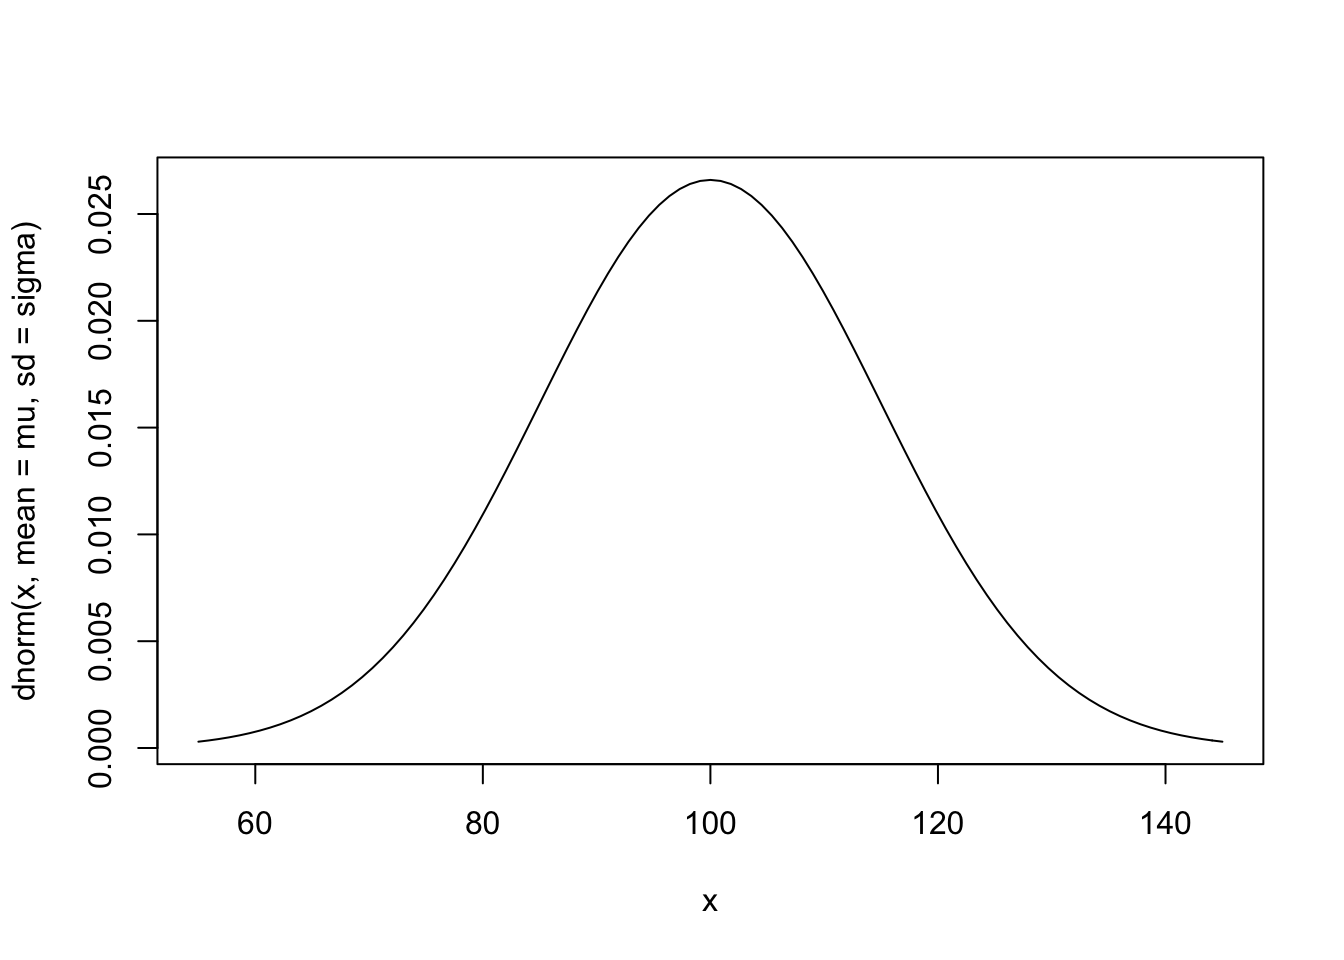
\includegraphics{_main_files/figure-latex/unnamed-chunk-72-1.pdf}

\begin{Shaded}
\begin{Highlighting}[]
\NormalTok{n0 \textless{}{-}}\StringTok{ }\DecValTok{25} \CommentTok{\# tamanho das amostras}
\NormalTok{n \textless{}{-}}\StringTok{ }\DecValTok{200} \CommentTok{\# número de amostras}
\KeywordTok{set.seed}\NormalTok{(}\DecValTok{1234}\NormalTok{) }\CommentTok{\# fixando semente pseudo{-}aleatória para garantir replicação}
\NormalTok{a \textless{}{-}}\StringTok{ }\NormalTok{MASS}\OperatorTok{::}\KeywordTok{mvrnorm}\NormalTok{(n0, }\DataTypeTok{mu =} \KeywordTok{rep}\NormalTok{(mu,n), }\DataTypeTok{Sigma =}\NormalTok{ sigma}\OperatorTok{\^{}}\DecValTok{2}\OperatorTok{*}\KeywordTok{diag}\NormalTok{(n)) }\CommentTok{\# amostras}
\NormalTok{ma \textless{}{-}}\StringTok{ }\KeywordTok{colMeans}\NormalTok{(a) }\CommentTok{\# médias das n amostras}
\KeywordTok{hist}\NormalTok{(ma) }\CommentTok{\# histograma das médias}
\end{Highlighting}
\end{Shaded}

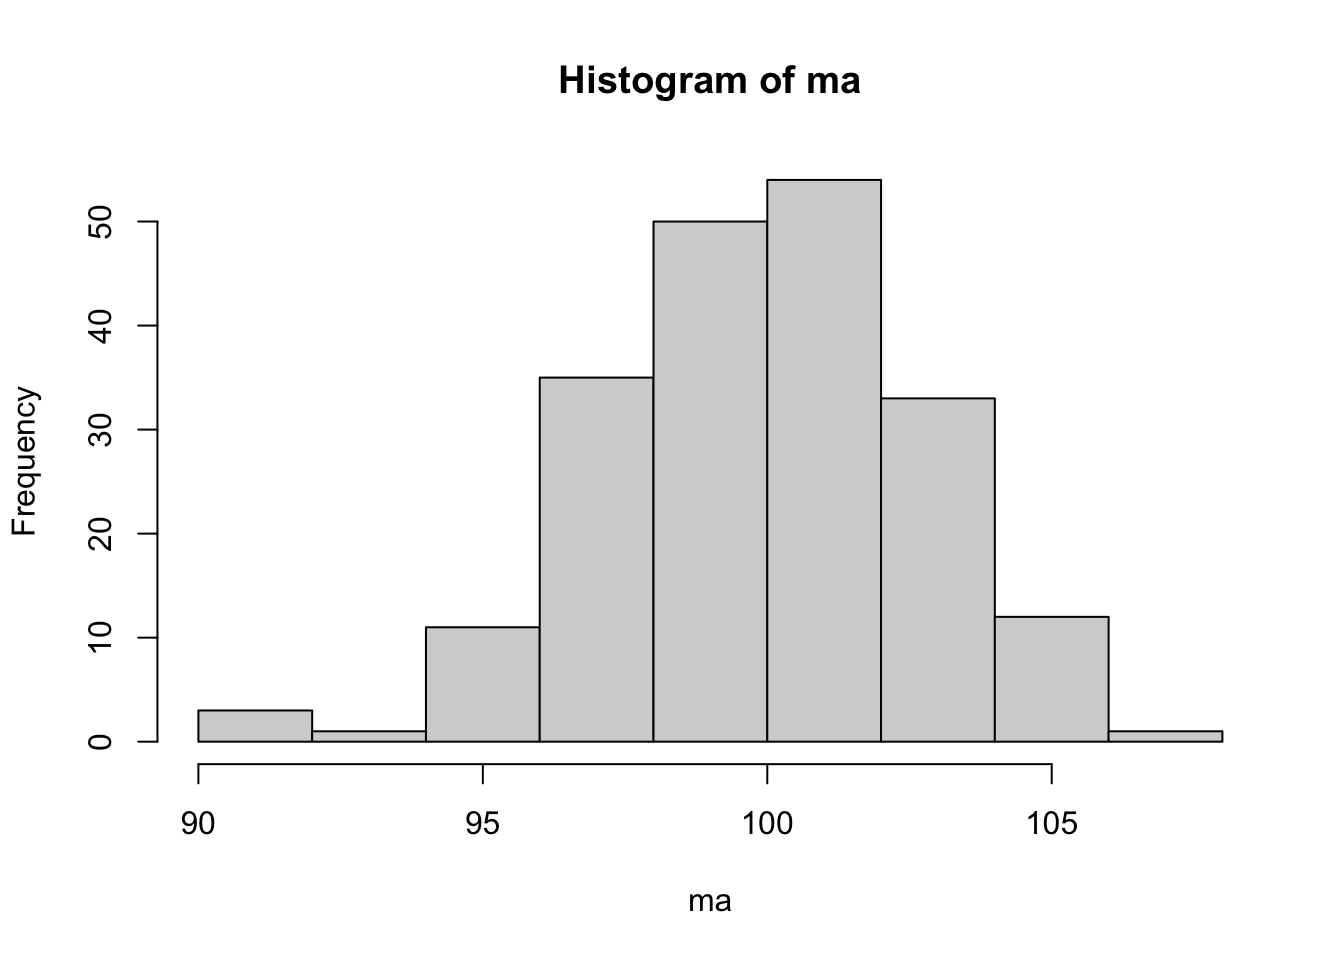
\includegraphics{_main_files/figure-latex/unnamed-chunk-72-2.pdf}

\begin{Shaded}
\begin{Highlighting}[]
\KeywordTok{mean}\NormalTok{(ma) }\CommentTok{\# média das médias amostrais, próxima de mu}
\end{Highlighting}
\end{Shaded}

\begin{verbatim}
## [1] 99.9
\end{verbatim}

\begin{Shaded}
\begin{Highlighting}[]
\KeywordTok{sd}\NormalTok{(ma) }\CommentTok{\# desvio padrão das médias, próximo de sigma/raiz(n0)}
\end{Highlighting}
\end{Shaded}

\begin{verbatim}
## [1] 2.82
\end{verbatim}

\begin{Shaded}
\begin{Highlighting}[]
\NormalTok{sigma}\OperatorTok{/}\KeywordTok{sqrt}\NormalTok{(n0) }\CommentTok{\# sigma/raiz(n0)}
\end{Highlighting}
\end{Shaded}

\begin{verbatim}
## [1] 3
\end{verbatim}

\begin{exercise}
\protect\hypertarget{exr:unnamed-chunk-73}{}{\label{exr:unnamed-chunk-73} }Refaça o Exemplo \ref{exm:qi} alterando os valores de \texttt{n0} e \texttt{n}, verificando o que ocorre no histograma, média e desvio padrão de \texttt{ma}. Atente para o fato de que valores de \texttt{n} maiores que 1000 podem tornar o processo custoso computacionalmente.
\end{exercise}

\hypertarget{amostra-representativa}{%
\subsection{Amostra representativa}\label{amostra-representativa}}

\begin{quote}
Ouve-se frequentemente o argumento de que uma boa amostra é aquela que é representativa. Indagado sobre a definição de uma amostra representativa, a resposta mais comum é algo como: ``aquela que é uma micro representação do universo''. Mas para se ter certeza de que uma amostra seja uma micro representação do universo para uma dada característica de interesse, deve-se conhecer o comportamento dessa mesma característica da população. Então, o conhecimento da população seria tão grande que tonar-se-ia desnecessária a coleta da amostra.\\
(Bolfarine and Bussab \protect\hyperlink{ref-bolfarine2005elementos}{2005}, 14)
\end{quote}

\hypertarget{tipos-de-amostras}{%
\subsection{Tipos de amostras}\label{tipos-de-amostras}}

\begin{figure}
\centering
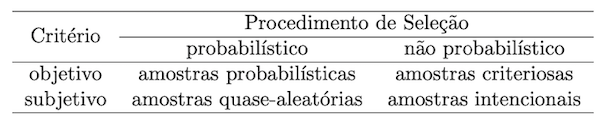
\includegraphics{img/criterio.png}
\caption{Tipos de amostras segundo (Bolfarine and Bussab \protect\hyperlink{ref-bolfarine2005elementos}{2005}) e (Jessen \protect\hyperlink{ref-jessen1978statistical}{1978}).}
\end{figure}

Procedimentos probabilísticos objetivos são mais bem aceitos academicamente, ainda que na prática nem sempre possam ser executados. Quando isso ocorre, podem-se considerar procedimentos que sejam possíveis de serem executados.

\hypertarget{principais-tuxe9cnicas-de-amostragem}{%
\section{Principais técnicas de amostragem}\label{principais-tuxe9cnicas-de-amostragem}}

\hypertarget{amostragem-aleatuxf3ria-simples}{%
\subsection{Amostragem Aleatória Simples}\label{amostragem-aleatuxf3ria-simples}}

\emph{Amostragem Aleatória Simples (AAS)} é o método mais básico de seleção de amostras, sendo referência para todos os demais planos amostrais. A partir de uma lista completa das \(N\) unidades elementares da população seleciona-se cada unidade amostral com igual probabilidade, de tal forma que a cada sorteio os elementos tenham a mesma chance de serem escolhidos. A necessidade de uma lista completa da população para realizar uma AAS pode eventualmente ser um limitante na aplicação deste tipo de metodologia, pois na prática nem sempre é possível obter tal listagem. Os planos amostrais A e B discutidos nos Exemplos \ref{exm:planos}, \ref{exm:aasc} e \ref{exm:aass} são caracterizados como AAS.

\hypertarget{aas-sem-reposiuxe7uxe3o---aass}{%
\subsubsection*{AAS sem reposição - AASs}\label{aas-sem-reposiuxe7uxe3o---aass}}
\addcontentsline{toc}{subsubsection}{AAS sem reposição - AASs}

Caso a unidade sorteada seja retirada da população e seja realizado um novo sorteio, é dito que procedeu-se com uma AAS \emph{restrita} ou \emph{sem reposição}, indicado por AASs.

\begin{example}
\protect\hypertarget{exm:urna-aass}{}{\label{exm:urna-aass} }(AASs) De uma urna com \(N\) cartões numerados de \(1\) a \(N\) sorteia-se um ao acaso, com probabilidade \(1/N\). O cartão sorteado é deixado de fora da urna e realiza-se um novo sorteio, onde cada um dos \(N-1\) cartões restantes tem probabilidade \(1/(N-1)\) de ser retirado. Este procedimento é repetido até que se concluam todos os \(n\) sorteios desejados. Este é um processo de AAS \emph{sem} reposição. \(\\\)
\end{example}

\begin{exercise}
\protect\hypertarget{exr:urna-aass-N}{}{\label{exr:urna-aass-N} }Defina as probabilidades de sorteio do Exemplo \ref{exm:urna-aass} considerando \(n=3\) sorteios. \(\\\)
\end{exercise}

\begin{exercise}
\protect\hypertarget{exr:urna-aass-10}{}{\label{exr:urna-aass-10} }Calcule as probabilidades de sorteio do Exemplo \ref{exm:urna-aass} considerando \(n=3\) sorteios e \(N=10\). \(\\\)
\end{exercise}

\begin{example}
\protect\hypertarget{exm:mega}{}{\label{exm:mega} }(Mega-Sena da Caixa Econômica Federal) No R pode-se sortear uma amostra sem reposição para tentar a sorte no jogo da Caixa Econômica Federal. Note que \(N=60\), \(n=6\).
\end{example}

\begin{Shaded}
\begin{Highlighting}[]
\KeywordTok{set.seed}\NormalTok{(}\DecValTok{1234}\NormalTok{) }\CommentTok{\# Fixando a geração pseudo{-}aleatória}
\KeywordTok{sort}\NormalTok{(}\KeywordTok{sample}\NormalTok{(}\DecValTok{1}\OperatorTok{:}\DecValTok{60}\NormalTok{, }\DataTypeTok{size =} \DecValTok{6}\NormalTok{, }\DataTypeTok{replace =}\NormalTok{ F)) }\CommentTok{\# Apostando na Mega{-}Sena da CEF via AASs}
\end{Highlighting}
\end{Shaded}

\begin{verbatim}
## [1] 16 22 28 37 44 58
\end{verbatim}

\begin{exercise}
\protect\hypertarget{exr:unnamed-chunk-75}{}{\label{exr:unnamed-chunk-75} }Leia a documentação das funções utilizadas no Exemplo \ref{exm:mega} fazendo \texttt{?set.seed},\\
\texttt{?sort} e \texttt{?sample}.
\end{exercise}

\hypertarget{aas-com-reposiuxe7uxe3o---aasc}{%
\subsubsection*{AAS com reposição - AASc}\label{aas-com-reposiuxe7uxe3o---aasc}}
\addcontentsline{toc}{subsubsection}{AAS com reposição - AASc}

Caso a unidade sorteada tenha a chance de participar novamente da amostra, o procedimento é chamado AAS \emph{irrestrita} ou \emph{com reposição}, indicado por AASc.

\begin{example}
\protect\hypertarget{exm:urna-aasc}{}{\label{exm:urna-aasc} }(AASc) De uma urna com \(N\) cartões numerados de \(1\) a \(N\) sorteia-se um ao acaso, com probabilidade \(1/N\). O cartão sorteado é recolocado na urna e realiza-se um novo sorteio. Este procedimento é repetido até que se concluam todos os \(n\) sorteios desejados. Este é um processo de AAS \emph{com} reposição. \(\\\)
\end{example}

\begin{exercise}
\protect\hypertarget{exr:urna-aasc-N}{}{\label{exr:urna-aasc-N} }Defina as probabilidades de sorteio do Exemplo \ref{exm:urna-aasc} considerando \(n=3\) sorteios. \(\\\)
\end{exercise}

\begin{exercise}
\protect\hypertarget{exr:urna-aasc-10}{}{\label{exr:urna-aasc-10} }Calcule as probabilidades de sorteio do Exemplo \ref{exm:urna-aasc} considerando \(n=3\) sorteios com \(N=10\). \(\\\)
\end{exercise}

\hypertarget{amostragem-sistemuxe1tica}{%
\subsection{Amostragem Sistemática}\label{amostragem-sistemuxe1tica}}

Considere uma população de \(N\) unidades elementares numeradas de 1 a \(N\). Para selecionar uma amostra de \(n\) observações sorteia-se aleatoriamente uma das primeiras \(k=N/n\) unidades, digamos \(a\), com probabilidade \(1/k\) selecionando sistematicamente as próximas observações a cada \(k\) unidades. Matematicamente, \[a, a+k, a+2k, \ldots, a+(n-1)k.\]

\begin{example}
\protect\hypertarget{exm:as}{}{\label{exm:as} }Seja uma população com \(N=100\), da qual deseja-se retirar uma amostra sistemática de tamanho \(n=5\). Neste caso \(k=100/5=20\), então sortearmos aleatoriamente um número entre 1 e 20 com probabilidade \(1/20\). Se o número sorteado for \(a=4\), a amostra sistemática então é definida como \[4, 4+20, 4+2 \times 20, 4+3 \times 20, 4+4 \times 20 = 4,24,44,64,84.\]
\end{example}

\begin{Shaded}
\begin{Highlighting}[]
\NormalTok{N \textless{}{-}}\StringTok{ }\DecValTok{100} \CommentTok{\# Tamanho da população}
\NormalTok{n \textless{}{-}}\StringTok{ }\DecValTok{5} \CommentTok{\# Tamanho da amostra}
\NormalTok{(k \textless{}{-}}\StringTok{ }\NormalTok{N}\OperatorTok{/}\NormalTok{n) }\CommentTok{\# Tamanho do salto}
\end{Highlighting}
\end{Shaded}

\begin{verbatim}
## [1] 20
\end{verbatim}

\begin{Shaded}
\begin{Highlighting}[]
\KeywordTok{set.seed}\NormalTok{(}\DecValTok{1}\NormalTok{) }\CommentTok{\# Fixando a geração pseudo{-}aleatória}
\NormalTok{(a \textless{}{-}}\StringTok{ }\KeywordTok{sample}\NormalTok{(}\DecValTok{1}\OperatorTok{:}\NormalTok{k, }\DataTypeTok{size =} \DecValTok{1}\NormalTok{)) }\CommentTok{\# Amostra de tamanho 1 com probabilidade 1/k}
\end{Highlighting}
\end{Shaded}

\begin{verbatim}
## [1] 4
\end{verbatim}

\begin{Shaded}
\begin{Highlighting}[]
\ControlFlowTok{for}\NormalTok{(i }\ControlFlowTok{in} \DecValTok{1}\OperatorTok{:}\NormalTok{n)\{}\KeywordTok{print}\NormalTok{(a}\OperatorTok{+}\NormalTok{(i}\DecValTok{{-}1}\NormalTok{)}\OperatorTok{*}\NormalTok{k)\} }\CommentTok{\# Apresentando a amostra de tamanho n}
\end{Highlighting}
\end{Shaded}

\begin{verbatim}
## [1] 4
## [1] 24
## [1] 44
## [1] 64
## [1] 84
\end{verbatim}

\begin{exercise}
\protect\hypertarget{exr:unnamed-chunk-77}{}{\label{exr:unnamed-chunk-77} }Considere o código do Exemplo \ref{exm:as}.\\
(a) Rode o código repetidas vezes retirando a linha \texttt{set.seed(1)}. O que você observa?\\
(b) Refaça o exercício considerando outros valores de \(N\) e \(n\), tais que \(n<N\).
\end{exercise}

\hypertarget{amostragem-estratificada}{%
\subsection{Amostragem Estratificada}\label{amostragem-estratificada}}

Segundo (Bolfarine and Bussab \protect\hyperlink{ref-bolfarine2005elementos}{2005}, 93),

\begin{quote}
Amostragem estratificada consiste na divisão de uma população em grupos (estratos) segundo alguma(s) característica(s) conhecida(s) na populaçãao sob estudo, e de cada um desses estratos são selecionadas amostras em proporções convenientes.
\end{quote}

O objetivo deste tipo de amostragem é que o pesquisador possa se valer de estruturas pré-existentes de maneira a melhorar as inferências, reduzindo sua variabilidade.

\hypertarget{cuxe1lculo-do-tamanho-da-amostra}{%
\section{Cálculo do tamanho da amostra}\label{cuxe1lculo-do-tamanho-da-amostra}}

O \emph{cálculo do tamanho de amostra} é baseado em uma série de premissas assumidas pelo pesquisador. Os valores sugeridos pelos diversos métodos de cálculo de tamanho de amostra devem ser considerados apenas como uma referência, dada a arbitrariedade das medidas utilizadas em sua obtenção. Tempo e custo são dois limitantes que devem ser levados em conta, podendo se sobrepor aos cálculos de tamanho de amostra.\\
A seguir serão apresentados casos bastante simples, mas suficientes para ilustrar os princípios utilizados. Para mais funcionalidades recomenda-se o pacote \texttt{pwr} (Champely \protect\hyperlink{ref-champely2020pwr}{2020}) do R e o software \href{https://www.gpower.hhu.de}{G*Power} (Franz Faul and Buchner \protect\hyperlink{ref-faul2007gpower}{2007}), (Franz Faul and Lang \protect\hyperlink{ref-faul2009gpower}{2009}). Para uma abordagem mais teórica recomenda-se (Chow, Wang, and Shao \protect\hyperlink{ref-chow2007sample}{2007}).

\hypertarget{muxe9dia}{%
\subsection{Média}\label{muxe9dia}}

Uma forma de estimar o tamanho da amostra no caso da inferência para a media universal \(\mu\) é considerar a margem de erro da Equação \eqref{eq:ic-media-sigma} e isolar \(n\) na forma
\begin{equation}
n = \left \lceil{ \left( \frac{z \sigma}{\varepsilon} \right)^2 }\right \rceil.
\label{eq:n-media-sigma}
\end{equation}

O operador \(\left \lceil{ x }\right \rceil\) indica a função \emph{teto} de \(x\), i.e., indica o primeiro inteiro acima de \(x\).

\begin{exercise}
\protect\hypertarget{exr:unnamed-chunk-78}{}{\label{exr:unnamed-chunk-78} }Obtenha o resultado da Equação \eqref{eq:n-media-sigma} a partir da margem de erro da Equação \eqref{eq:ic-media-sigma}. \(\\\)
\end{exercise}

\begin{example}
\protect\hypertarget{exm:n-media-95}{}{\label{exm:n-media-95} }(Tamanho da amostra para a média) Deseja-se obter o tamanho de amostra para estimar a média de altura dos alunos da PUCRS. Considera-se um intervalo de confiança de \(1-\alpha = 95\%\), com margem de erro de \(\varepsilon = 3\) cm. De estudos anteriores, admite-se \(\sigma = 15\) cm. Considerando a Equação \eqref{eq:n-media-sigma}, sabe-se da tabela da distribuição normal padrão que \(z = 1.96\), assim
\begin{equation}
n = \left \lceil{ \left( \frac{1.96 \times 15}{3} \right)^2 }\right \rceil = \left \lceil{ 96.04 }\right \rceil = 97.
\label{eq:n-media-95}
\end{equation}
\end{example}

\begin{Shaded}
\begin{Highlighting}[]
\CommentTok{\# Equação (3.8)}
\NormalTok{n\_m \textless{}{-}}\StringTok{ }\ControlFlowTok{function}\NormalTok{(z,sigma,e) \{}
\NormalTok{  exato \textless{}{-}}\StringTok{ }\NormalTok{(z}\OperatorTok{*}\NormalTok{sigma}\OperatorTok{/}\NormalTok{e)}\OperatorTok{\^{}}\DecValTok{2}     
\NormalTok{  teto \textless{}{-}}\StringTok{ }\KeywordTok{ceiling}\NormalTok{(exato)}
  \KeywordTok{return}\NormalTok{(}\KeywordTok{list}\NormalTok{(}\DataTypeTok{exato=}\NormalTok{exato, }
              \DataTypeTok{teto=}\NormalTok{teto))}
\NormalTok{\}      }
\KeywordTok{n\_m}\NormalTok{(}\FloatTok{1.96}\NormalTok{,}\DecValTok{15}\NormalTok{,}\DecValTok{3}\NormalTok{)}
\end{Highlighting}
\end{Shaded}

\begin{verbatim}
## $exato
## [1] 96
## 
## $teto
## [1] 97
\end{verbatim}

\begin{Shaded}
\begin{Highlighting}[]
\KeywordTok{n\_m}\NormalTok{(}\FloatTok{1.96}\NormalTok{,}\DecValTok{15}\NormalTok{,}\DecValTok{3}\NormalTok{)}\OperatorTok{$}\NormalTok{exato}
\end{Highlighting}
\end{Shaded}

\begin{verbatim}
## [1] 96
\end{verbatim}

\begin{Shaded}
\begin{Highlighting}[]
\KeywordTok{n\_m}\NormalTok{(}\FloatTok{1.96}\NormalTok{,}\DecValTok{15}\NormalTok{,}\DecValTok{3}\NormalTok{)}\OperatorTok{$}\NormalTok{teto}
\end{Highlighting}
\end{Shaded}

\begin{verbatim}
## [1] 97
\end{verbatim}

\hypertarget{proporuxe7uxe3o}{%
\subsection{Proporção}\label{proporuxe7uxe3o}}

Uma forma de estimar o tamanho da amostra no caso da inferência para a proporção universal \(\pi\) é considerar a margem de erro da Equação \eqref{eq:ic-prop} e isolar \(n\) na forma
\begin{equation}
n = \left \lceil{ \frac{z^2 p (1-p)}{\varepsilon^2} }\right \rceil.
\label{eq:n-prop}
\end{equation}

Em certos casos existe informação disponível sobre a proporção, mas quando não há qualquer conhecimento a respeito desta medida considera-se \(p=\frac{1}{2}\), ponto no qual \(p(1-p)\) atinge seu máximo.

\begin{exercise}
\protect\hypertarget{exr:unnamed-chunk-80}{}{\label{exr:unnamed-chunk-80} }Obtenha o resultado da Equação \eqref{eq:n-prop} a partir da margem de erro da Equação \eqref{eq:ic-prop}. \(\\\)
\end{exercise}

\begin{exercise}
\protect\hypertarget{exr:unnamed-chunk-81}{}{\label{exr:unnamed-chunk-81} }Verifique que \(p(1-p)\) atinge seu máximo quando \(p=\frac{1}{2}\). \(\\\)
\end{exercise}

\begin{example}
\protect\hypertarget{exm:n-prop-95}{}{\label{exm:n-prop-95} }(Tamanho da amostra para a proporção) Em uma pesquisa eleitoral deseja-se calcular o tamanho de amostra aproximado para que a margem de erro seja de \(\varepsilon = 2\%\) com confiança de \(1-\alpha = 95\%\). Considerando a Equação \eqref{eq:n-prop}, sabe-se da tabela da distribuição normal padrão que \(z = 1.96 \approx 2\), e que \(p(1-p)\) atinge seu máximo quando \(p=\frac{1}{2}\). Assim,
\begin{equation}
n \approx \left \lceil{ \frac{2^2 \times \frac{1}{2} \times (1-\frac{1}{2})}{\varepsilon^2} }\right \rceil = \left \lceil{ \frac{1}{\varepsilon^2} }\right \rceil
\label{eq:n-prop-95}
\end{equation}

Logo, um IC para a proporção com \(\alpha = 5\%\) para uma margem de erro de \(\varepsilon = 2\%\) pode ser calculado com um tamanho de amostra de aproximadamente \[ n \approx \left \lceil{ \frac{1}{0.02^2} }\right \rceil = 2500. \]
\end{example}

\begin{Shaded}
\begin{Highlighting}[]
\CommentTok{\# Equação (3.11)}
\NormalTok{n\_p \textless{}{-}}\StringTok{ }\ControlFlowTok{function}\NormalTok{(e) \{}
\NormalTok{  exato \textless{}{-}}\StringTok{ }\DecValTok{1}\OperatorTok{/}\NormalTok{e}\OperatorTok{\^{}}\DecValTok{2}
\NormalTok{  teto \textless{}{-}}\StringTok{ }\KeywordTok{ceiling}\NormalTok{(exato)}
  \KeywordTok{return}\NormalTok{(}\KeywordTok{list}\NormalTok{(}\DataTypeTok{exato=}\NormalTok{exato, }
              \DataTypeTok{teto=}\NormalTok{teto))}
\NormalTok{\}      }
\KeywordTok{n\_p}\NormalTok{(}\FloatTok{0.02}\NormalTok{)}
\end{Highlighting}
\end{Shaded}

\begin{verbatim}
## $exato
## [1] 2500
## 
## $teto
## [1] 2500
\end{verbatim}

\begin{Shaded}
\begin{Highlighting}[]
\KeywordTok{n\_p}\NormalTok{(}\FloatTok{0.02}\NormalTok{)}\OperatorTok{$}\NormalTok{exato}
\end{Highlighting}
\end{Shaded}

\begin{verbatim}
## [1] 2500
\end{verbatim}

\begin{Shaded}
\begin{Highlighting}[]
\KeywordTok{n\_p}\NormalTok{(}\FloatTok{0.02}\NormalTok{)}\OperatorTok{$}\NormalTok{teto}
\end{Highlighting}
\end{Shaded}

\begin{verbatim}
## [1] 2500
\end{verbatim}

\begin{exercise}
\protect\hypertarget{exr:unnamed-chunk-83}{}{\label{exr:unnamed-chunk-83} }Teste a função \texttt{n\_p} do Exemplo \ref{exm:n-prop-95} com diferentes valores de margem de erro. Faça um gráfico para analisar a variação do tamanho da amostra à medida que \(\varepsilon\) aumenta. \(\\\)
\end{exercise}

\hypertarget{para-saber-mais}{%
\section{Para saber mais}\label{para-saber-mais}}

O material \href{https://amostragemcomr.github.io/livro/index.html}{Amostragem: Teoria e Prática Usando R}, gentilmente disponibilizado pelos professores Pedro Luis do Nascimento Silva, Zélia Magalhães Bianchini e Antonio José Ribeiro Dias, é uma fonte muito rica para informações adicionais sobre este tópico. Está disponível ainda o livro \href{https://djalmapessoa.github.io/adac/}{Análise de Dados Amostrais Complexos}, também do professor Pedro Silva em parceria com o professor Djalma Pessoa.\\
O professor Pedro também compartilhou o \href{https://www.youtube.com/watch?v=_s9b8fQ7uEA}{vídeo} e os \href{https://drive.google.com/file/d/1cST0mA_nrYI2HZz9tgIAho4oHHYX42D4/view}{slides} da apresentação \emph{Combinando amostras para aprimorar estimativas -- aventuras na amostragem não probabilística}, apresentado em 18 de outubro de 2020 no \emph{VII Encontro Baiano de Estatística}.

\hypertarget{inferencia-classica}{%
\chapter{Inferência Clássica}\label{inferencia-classica}}

\emph{Inferência} é o procedimento que visa atualizar a informação sobre parâmetros a partir dos dados amostrais. Para (DeGroot and Schervish \protect\hyperlink{ref-degroot2012probability}{2012}, 378), `inferência estatística é um procedimento que produz uma declaração probabilística a respeito de uma ou mais partes de um modelo estatístico'\footnote{`\emph{A statistical inference is a procedure that produces a probabilistic statement about some or all parts of a statistical model.}'}. Conclusões obtidas a partir dos dados embasam a \emph{lógica indutiva}, i.e., aquela que parte do caso particular para o caso geral e que se opõe à \emph{lógica dedutiva} que vai do caso geral para o particular. O princípio indutivo se enquadra na noção de um decisor, a partir de uma amostra (caso particular), \emph{inferir} sobre parâmetros universais/populacionais.

(Berger \protect\hyperlink{ref-berger1985statistical}{1985}, 16) e (Paulino, Turkman, and Murteira \protect\hyperlink{ref-paulino2003estatistica}{2003}, 6) indicam que os procedimentos baseados no \emph{paradigma clássico} baseiam-se em alguns princípios, tais como máxima verossimilhança, não viés\footnote{Definição \ref{def:unbiased}.}, variância mínima, mínimos quadrados, consistência, suficiência e eficiência. Os clássicos consideram que existe um parâmetro \(\theta\) desconhecido para o qual não se atribui probabilidades. A amostra é obtida \emph{aleatoriamente} de um universo de interesse, sendo uma das tantas - se não infinitas - possíveis amostras. (Berger \protect\hyperlink{ref-berger1985statistical}{1985}, 26) aponta que tal princípio coloca os clássicos como \emph{incondicionalistas}, pois pondera-se sobre todos os dados possíveis e não condicionado ao que foi observado.

A abordagem clássica possui três tipos de estimação: \emph{Pontual} (ou \emph{por ponto}), por \emph{Intervalo de Confiança} (IC/ICo) e por \emph{Teste de Hipóteses} (TH), detalhadas a seguir.

\hypertarget{estimauxe7uxe3o-pontual}{%
\section{Estimação Pontual}\label{estimauxe7uxe3o-pontual}}

Na \emph{estimação pontual} utiliza-se uma estatística, calculada a partir de um \emph{estimador} como \emph{estimativa} (\emph{pontual}) de um certo parâmetro, conforme Definição \ref{def:estimador} e \ref{def:estimativa}. Em outras palavras, é utilizado um único valor amostral (ponto) para estimar \(\theta\), simbolizado por \(\hat{\theta}\) e lido como \emph{teta chapéu}.

\begin{definition}
\protect\hypertarget{def:estimador}{}{\label{def:estimador} }Um \emph{estimador} \(\hat{\theta}(\boldsymbol{x}) \equiv \hat{\theta}\) é uma função que tem por objetivo inferir sobre um parâmetro \(\theta(\boldsymbol{X}) \equiv \theta\). \(\\\)
\end{definition}

\begin{definition}
\protect\hypertarget{def:estimativa}{}{\label{def:estimativa} }Uma \emph{estimativa} é um particular valor obtido da aplicação dos dados amostrais em um estimador. \(\\\)
\end{definition}

\begin{example}
\protect\hypertarget{exm:media-am}{}{\label{exm:media-am} }A média amostral \(\bar{x}\) é um estimador pontual para a média universal \(\mu\) (Eq. \eqref{eq:media-univ}). É dado pela Equação \eqref{eq:media-am}.
\end{example}

\hypertarget{estimadores-e-suas-propriedades}{%
\subsection{Estimadores e suas propriedades}\label{estimadores-e-suas-propriedades}}

\begin{definition}
\protect\hypertarget{def:unbiased}{}{\label{def:unbiased} }Um estimador é dito \emph{não viesado} ou \emph{não viciado} segundo um plano amostral \(\lambda\) se
\begin{equation} 
E_\lambda \left[ \hat{\theta} \right] = \theta.
\label{eq:unbiased}
\end{equation}
\end{definition}

\hypertarget{muxe9dia-amostral-barx}{%
\subsubsection*{\texorpdfstring{Média amostral \(\bar{x}\)}{Média amostral \textbackslash bar\{x\}}}\label{muxe9dia-amostral-barx}}
\addcontentsline{toc}{subsubsection}{Média amostral \(\bar{x}\)}

A média amostral do Exemplo \eqref{eq:media-am} é um estimador não viesado da média universal \(\mu\) segundo o plano amostral AAS, com ou sem reposição. Isto ocorre pelo fato de a esperança ser linear, portanto a dependência entre as observações não interfere no resultado. \(\\\)
\begin{example}
\protect\hypertarget{exm:unbiased-media}{}{\label{exm:unbiased-media} }Sejam as variáveis aleatórias \(X_1, X_2, \ldots, X_n\) independentes identicamente distribuídas (iid) com \(E(X_i)=\mu\) e um plano amostral do tipo AAS, onde por simplicidade será considerada a equivalência \(E_{AAS} \equiv E\).
\begin{align*}
E\left[\bar{x}\right] &= E\left[\frac{1}{n} \sum_{i=1}^{n} x_i \right] \\
                      &= \frac{1}{n} E\left[\sum_{i=1}^{n} x_i \right] \\
                      &= \frac{1}{n} \sum_{i=1}^{n} E\left[x_i \right] \\
                      &= \frac{1}{n} \sum_{i=1}^{n} \mu \\
                      &= \frac{1}{n} n\mu \\
E\left[\bar{x}\right] &= \mu.
\label{eq:unbiased-media}
\end{align*}
\end{example}

\begin{example}
\protect\hypertarget{exm:unbiased-media-aasc}{}{\label{exm:unbiased-media-aasc} }A média universal da variável \texttt{idade} do Exemplo \ref{exm:universo} é dada por \[\mu = \frac{24+32+49}{3} = \frac{105}{3} = 35.\]
Do Exemplo \ref{exm:aasc} pode-se verificar que a média (esperança) das médias amostrais considerando o plano AASc é igual a \(\mu\), i.e., \[E\left[h(\boldsymbol{x})\right] = E\left[\bar{x}\right] = \frac{24.0+28.0+36.5+28.0+32.0+40.5+36.5+40.5+49.0}{9}=\frac{315}{9}=35.\]
\end{example}

\begin{Shaded}
\begin{Highlighting}[]
\NormalTok{X \textless{}{-}}\StringTok{ }\KeywordTok{c}\NormalTok{(}\DecValTok{24}\NormalTok{,}\DecValTok{32}\NormalTok{,}\DecValTok{49}\NormalTok{)}
\KeywordTok{mean}\NormalTok{(X)}
\end{Highlighting}
\end{Shaded}

\begin{verbatim}
## [1] 35
\end{verbatim}

Do Exemplo \ref{exm:aas-R} tem-se o vetor \texttt{mxc\ \textless{}-\ c(24.0,28.0,36.5,28.0,32.0,40.5,36.5,40.5,49.0)}.

\begin{Shaded}
\begin{Highlighting}[]
\KeywordTok{mean}\NormalTok{(mxc)}
\end{Highlighting}
\end{Shaded}

\begin{verbatim}
## [1] 35
\end{verbatim}

\begin{exercise}
\protect\hypertarget{exr:unnamed-chunk-86}{}{\label{exr:unnamed-chunk-86} }Verifique no plano amostral AASs do Exemplo \ref{exm:aass} que \(E\left[\bar{x}\right] = \mu\). \(\\\)
\end{exercise}

\hypertarget{proporuxe7uxe3o-amostral-p}{%
\subsubsection*{\texorpdfstring{Proporção amostral \(p\)}{Proporção amostral p}}\label{proporuxe7uxe3o-amostral-p}}
\addcontentsline{toc}{subsubsection}{Proporção amostral \(p\)}

A \emph{proporção amostral} é um estimador não viesado da proporção universal \(\pi\) (Eq. \eqref{eq:prop-univ}) segundo o plano amostral AAS, com ou sem reposição. Pode-se definir este estimador por
\begin{align*}
p = \frac{\sum_{i=1}^n x_i}{n}
\label{eq:prop-am}
\end{align*}

\begin{example}
\protect\hypertarget{exm:prop-fum}{}{\label{exm:prop-fum} }(Estimativa pontual da proporção) Suponha que deseja-se calcular a estimativa pontual para a `proporção de fumantes da PUCRS', denotada por \(\pi\). A característica de interesse, ou sucesso, é o entrevistado ser `fumante', para o qual associa-se \(x=1\); desta forma, o fracasso é o entrevistado ser `não fumante', para o qual associa-se \(x=0\). Em uma amostra de \(n = 125\) frequentadores da universidade, observaram-se \(\sum_{i=1}^n x_i = 25\) fumantes. A estimativa pontual de \(\pi\) é dada por \[ \hat{\pi} = \dfrac{25}{125} = 0.2 = 20\%. \]
\end{example}

\hypertarget{variuxe2ncia-amostral-s2}{%
\subsubsection*{\texorpdfstring{Variância amostral \(s^2\)}{Variância amostral s\^{}2}}\label{variuxe2ncia-amostral-s2}}
\addcontentsline{toc}{subsubsection}{Variância amostral \(s^2\)}

A variância amostral é um estimador não viesado da variância universal \(\sigma^2\) segundo o plano amostral AAS com reposição. \(\\\)
\begin{example}
\protect\hypertarget{exm:unbiased-var}{}{\label{exm:unbiased-var} }Sejam as variáveis aleatórias \(X_1, X_2, \ldots, X_n\) independentes identicamente distribuídas (iid) com \(E(X_i)=\mu\), \(Var(X_i)=\sigma^2\), \(E(X_{i}^2)=\sigma^2+\mu^2\) e um plano amostral do tipo AASc, onde por simplicidade será considerada a equivalência \(E_{AASc} \equiv E\).
\begin{align*}
E\left[s^2\right] &= E\left[\frac{1}{n-1} \sum_{i=1}^{n} (x_{i}-\bar{y})^2 \right] \\
                  &= \frac{1}{n-1} E\left[\sum_{i=1}^{n} x_{i}^2 -2 \bar{x} \sum_{i=1}^{n} x_{i} + n\bar{x}^2 \right] \\
                  &= \frac{1}{n-1} \left[\sum_{i=1}^{n} E\left[x_{i}^2\right] - E\left[n\bar{x}^2\right] \right] \\
                  &= \frac{1}{n-1} \left[\sum_{i=1}^{n} E\left[x_{i}^2\right] - nE\left[\bar{x}^2\right] \right] \\
                  &= \frac{1}{n-1} \left[n\sigma^2 + n\mu^2 - \sigma^2 - n\mu^2\right] \\
                  &= \frac{(n-1)\sigma^2}{n-1} \\
E\left[s^2\right] &= \sigma^2
\label{eq:unbiased-media}
\end{align*}
\end{example}

\begin{exercise}
\protect\hypertarget{exr:unnamed-chunk-87}{}{\label{exr:unnamed-chunk-87} }Verifique no plano amostral AASc do Exemplo \ref{exm:aasc} se \(E_{AASc}\left[s^2\right] = \sigma^2\). \(\\\)
\end{exercise}

\begin{exercise}
\protect\hypertarget{exr:unnamed-chunk-88}{}{\label{exr:unnamed-chunk-88} }Verifique no plano amostral AASs do Exemplo \ref{exm:aass} se \(E_{AASs}\left[s^2\right] = \sigma^2\). \(\\\)
\end{exercise}

\hypertarget{estimauxe7uxe3o-por-intervalo-de-confianuxe7a}{%
\section{(Estimação por) Intervalo de Confiança}\label{estimauxe7uxe3o-por-intervalo-de-confianuxe7a}}

\hypertarget{muxe9dia-1}{%
\subsection{Média}\label{muxe9dia-1}}

\hypertarget{sigma-conhecido}{%
\subsubsection*{\texorpdfstring{\(\sigma\) conhecido}{\textbackslash sigma conhecido}}\label{sigma-conhecido}}
\addcontentsline{toc}{subsubsection}{\(\sigma\) conhecido}

O IC para a média universal com \(\sigma\) conhecido é dado pela expressão
\begin{equation}
IC \left[ \mu, 1-\alpha \right] = \bar{x} \mp z \dfrac{\sigma}{\sqrt{n}} = \left[ \bar{x} - z \dfrac{\sigma}{\sqrt{n}}, \bar{x} + z \dfrac{\sigma}{\sqrt{n}} \right],
\label{eq:ic-media-sigma}
\end{equation}
onde \(1-\alpha\) é a confiança do intervalo, \(\bar{x}\) é a média amostral, \(\sigma\) é o desvio padrão universal conhecido, \(n\) é o tamanho da amostra e \(z=z_{\frac{\alpha}{2}}\) é o quantil da distribuição normal padrão que acumula \(\frac{\alpha}{2}\) de probabilidade.

\begin{example}
\protect\hypertarget{exm:ic-media-sigma}{}{\label{exm:ic-media-sigma} }(IC para \(\mu\) com \(\sigma\) conhecido) Considere uma amostra de \(n=10\) mulheres, das quais observou-se a variável \(X\): `altura'. Suponha que \(X \sim \mathcal{N}(\mu,0.05)\), i.e., a variável `altura das mulheres' tem distribuição normal com média \(\mu\) desconhecida e desvio padrão universal conhecido \(\sigma = 0.05\). Da tabela da distribuição normal sabe-se que os quantis \(\pm 1.96\) limitam uma área de aproximadamente \(95\%\), portanto \(z=1.96\). Se a média da amostra é \(\bar{x}_{10} = 1.63\), o IC de \(1-\alpha=95\%\) é \[ IC \left[ \mu, 95\% \right] = 1.63 \mp 1.96 \dfrac{0.05}{\sqrt{10}} \approx 1.63 \mp 0.03 \approx \left[ 1.60, 1.66 \right]. \] A margem de erro é de aproximadamente \(0.03\) ou 3 cm.
\end{example}

\begin{Shaded}
\begin{Highlighting}[]
\NormalTok{n \textless{}{-}}\StringTok{ }\DecValTok{10}
\NormalTok{m \textless{}{-}}\StringTok{ }\FloatTok{1.63}
\NormalTok{sigma \textless{}{-}}\StringTok{ }\FloatTok{0.05}                   \CommentTok{\# \textquotesingle{}sigma\textquotesingle{} universal}
\NormalTok{z \textless{}{-}}\StringTok{ }\KeywordTok{abs}\NormalTok{(}\KeywordTok{qnorm}\NormalTok{(}\FloatTok{0.025}\NormalTok{))          }\CommentTok{\# |{-}1.959964|}
\NormalTok{(e \textless{}{-}}\StringTok{ }\NormalTok{z}\OperatorTok{*}\NormalTok{sigma}\OperatorTok{/}\KeywordTok{sqrt}\NormalTok{(n))          }\CommentTok{\# Margem de erro}
\end{Highlighting}
\end{Shaded}

\begin{verbatim}
## [1] 0.031
\end{verbatim}

\begin{Shaded}
\begin{Highlighting}[]
\NormalTok{(LImusig \textless{}{-}}\StringTok{ }\NormalTok{m }\OperatorTok{{-}}\StringTok{ }\NormalTok{e)              }\CommentTok{\# Limite Inferior}
\end{Highlighting}
\end{Shaded}

\begin{verbatim}
## [1] 1.6
\end{verbatim}

\begin{Shaded}
\begin{Highlighting}[]
\NormalTok{(LSmusig \textless{}{-}}\StringTok{ }\NormalTok{m }\OperatorTok{+}\StringTok{ }\NormalTok{e)              }\CommentTok{\# Limite Superior}
\end{Highlighting}
\end{Shaded}

\begin{verbatim}
## [1] 1.66
\end{verbatim}

\begin{Shaded}
\begin{Highlighting}[]
\CommentTok{\# Princípio de relatório automático}
\KeywordTok{cat}\NormalTok{(}\StringTok{\textquotesingle{}O IC 95\% para a média é [\textquotesingle{}}\NormalTok{, }
    \KeywordTok{round}\NormalTok{(LImusig,}\DecValTok{2}\NormalTok{), }\StringTok{\textquotesingle{},\textquotesingle{}}\NormalTok{, }
    \KeywordTok{round}\NormalTok{(LSmusig,}\DecValTok{2}\NormalTok{), }\StringTok{\textquotesingle{}].\textquotesingle{}}\NormalTok{)}
\end{Highlighting}
\end{Shaded}

\begin{verbatim}
## O IC 95% para a média é [ 1.6 , 1.66 ].
\end{verbatim}

\hypertarget{sigma-desconhecido}{%
\subsubsection*{\texorpdfstring{\(\sigma\) desconhecido}{\textbackslash sigma desconhecido}}\label{sigma-desconhecido}}
\addcontentsline{toc}{subsubsection}{\(\sigma\) desconhecido}

O IC para a média universal com \(\sigma\) desconhecido é dado pela expressão
\begin{eqnarray}
IC \left[ \mu, 1-\alpha \right] = \bar{x} \mp t \dfrac{s}{\sqrt{n}} = \left[ \bar{x} - t \dfrac{s}{\sqrt{n}}, \bar{x} + t \dfrac{s}{\sqrt{n}} \right],
\label{eq:ic-media-s}
\end{eqnarray}
onde \(1-\alpha\) é a confiança do intervalo, \(\bar{x}\) é a média amostral, \(s\) é o desvio padrão amostral, \(n\) é o tamanho da amostra e \(t=t_{n-1, \frac{\alpha}{2}}\) é o quantil da distribuição \(t\) com \(n-1\) graus de liberdade que acumula \(1-\frac{\alpha}{2}\) de probabilidade. Note a troca de \(\sigma\) por \(s\), implicando na penalidade de utilizar \(t\) no lugar de \(z\).

\begin{example}
\protect\hypertarget{exm:ic-media-s}{}{\label{exm:ic-media-s} }(IC para \(\mu\) com \(\sigma\) desconhecido) Assim como no Exemplo \ref{exm:ic-media-sigma}, considere uma amostra de \(n=10\) mulheres das quais observou-se a variável \(X\): `altura'. Suponha que \(X \sim \mathcal{N}(\mu,\sigma)\), i.e., a variável `altura das mulheres' tem distribuição normal com média \(\mu\) e desvio padrão universal \(\sigma\), ambos desconhecidos. Da tabela da distribuição \(t\) com \(10-1=9\) graus de liberdade, sabe-se que os quantis \(\pm 2.262\) limitam uma área de aproximadamente \(95\%\), portanto \(t=2.262\). Se da amostra calculou-se média de \(\bar{x}_{10} = 1.63\) e desvio padrão de \(s=0.05\), o IC de \(1-\alpha=95\%\) é \[ IC \left[ \mu, 95\% \right] = 1.63 \mp 2.262 \dfrac{0.05}{\sqrt{10}} \approx 1.63 \mp 0.04 \approx \left[ 1.59, 1.67 \right]. \] A margem de erro é de aproximadamente \(0.04\) ou 4 cm, maior que a margem de erro \(0.03\) quando assume-se \(\sigma\) conhecido pois \(z=1.96 < 2.262=t\).
\end{example}

\begin{Shaded}
\begin{Highlighting}[]
\NormalTok{n \textless{}{-}}\StringTok{ }\DecValTok{10}
\NormalTok{m \textless{}{-}}\StringTok{ }\FloatTok{1.63}
\NormalTok{s \textless{}{-}}\StringTok{ }\FloatTok{0.05}                       \CommentTok{\# \textquotesingle{}s\textquotesingle{} amostral}
\NormalTok{t \textless{}{-}}\StringTok{ }\KeywordTok{abs}\NormalTok{(}\KeywordTok{qt}\NormalTok{(}\FloatTok{0.025}\NormalTok{, n}\DecValTok{{-}1}\NormalTok{))        }\CommentTok{\# |{-}2.2621572|}
\NormalTok{(e \textless{}{-}}\StringTok{ }\NormalTok{t}\OperatorTok{*}\NormalTok{s}\OperatorTok{/}\KeywordTok{sqrt}\NormalTok{(n))              }\CommentTok{\# Margem de erro}
\end{Highlighting}
\end{Shaded}

\begin{verbatim}
## [1] 0.0358
\end{verbatim}

\begin{Shaded}
\begin{Highlighting}[]
\NormalTok{(LImus \textless{}{-}}\StringTok{ }\NormalTok{m }\OperatorTok{{-}}\StringTok{ }\NormalTok{e)                }\CommentTok{\# Limite Inferior}
\end{Highlighting}
\end{Shaded}

\begin{verbatim}
## [1] 1.59
\end{verbatim}

\begin{Shaded}
\begin{Highlighting}[]
\NormalTok{(LSmus \textless{}{-}}\StringTok{ }\NormalTok{m }\OperatorTok{+}\StringTok{ }\NormalTok{e)                }\CommentTok{\# Limite Superior}
\end{Highlighting}
\end{Shaded}

\begin{verbatim}
## [1] 1.67
\end{verbatim}

\begin{Shaded}
\begin{Highlighting}[]
\CommentTok{\# Princípio de relatório automático}
\KeywordTok{cat}\NormalTok{(}\StringTok{\textquotesingle{}O IC 95\% para a média é [\textquotesingle{}}\NormalTok{, }
    \KeywordTok{round}\NormalTok{(LImus,}\DecValTok{2}\NormalTok{), }\StringTok{\textquotesingle{},\textquotesingle{}}\NormalTok{, }
    \KeywordTok{round}\NormalTok{(LSmus,}\DecValTok{2}\NormalTok{), }\StringTok{\textquotesingle{}].\textquotesingle{}}\NormalTok{)}
\end{Highlighting}
\end{Shaded}

\begin{verbatim}
## O IC 95% para a média é [ 1.59 , 1.67 ].
\end{verbatim}

\hypertarget{proporuxe7uxe3o-1}{%
\subsection{Proporção}\label{proporuxe7uxe3o-1}}

O IC para a proporção populacional \(\pi\) é dado pela expressão
\begin{equation}
IC \left[ \pi, 1-\alpha \right] = p \mp z \sqrt{\dfrac{p(1-p)}{n}} = \left[ p - z \sqrt{\dfrac{p(1-p)}{n}}, p + z \sqrt{\dfrac{p(1-p)}{n}} \right]
\label{eq:ic-prop}
\end{equation}
onde \(1-\alpha\) é a confiança do intervalo, \(p\) é a proporção amostral, \(n\) é o tamanho da amostra e \(z=z_{\frac{\alpha}{2}}\) é o quantil da distribuição normal padrão que acumula \(\frac{\alpha}{2}\) de probabilidade.

\begin{example}
\protect\hypertarget{exm:ic-prop}{}{\label{exm:ic-prop} }(IC para \(\pi\)) Considere novamente os dados do Exemplo \ref{exm:prop-fum}, onde deseja-se calcular o IC para a proporção de fumantes da PUCRS. Sabe-se que \(\hat{\pi} = p = 25/125 = 0.2\), \(n=125\) e \(z=1.96\). O IC de \(1-\alpha=95\%\) é \[ IC \left[ \pi, 95\% \right] = 0.2 \mp 1.96 \sqrt{\dfrac{0.2 \left(  1-0.2 \right)  }{125}} \approx 0.2 \mp 0.07 = \left[ 0.13, 0.27 \right] = \left[ 13\%, 27\% \right]. \] A margem de erro é de aproximadamente \(0.07 = 7\%\), Note a diferença de precisão entre a tabela, consultando a probabilidade 0.0250 correspondente a \(z=-1.96\), e o valor calculado com a função \texttt{qnorm}.
\end{example}

\begin{Shaded}
\begin{Highlighting}[]
\NormalTok{n \textless{}{-}}\StringTok{ }\DecValTok{125}
\NormalTok{p \textless{}{-}}\StringTok{ }\DecValTok{25}\OperatorTok{/}\NormalTok{n}
\NormalTok{z \textless{}{-}}\StringTok{ }\KeywordTok{abs}\NormalTok{(}\KeywordTok{qnorm}\NormalTok{(}\FloatTok{0.025}\NormalTok{))          }\CommentTok{\# |{-}1.959964|}
\NormalTok{(e \textless{}{-}}\StringTok{ }\NormalTok{z}\OperatorTok{*}\KeywordTok{sqrt}\NormalTok{(p}\OperatorTok{*}\NormalTok{(}\DecValTok{1}\OperatorTok{{-}}\NormalTok{p)}\OperatorTok{/}\NormalTok{n))        }\CommentTok{\# Margem de erro}
\end{Highlighting}
\end{Shaded}

\begin{verbatim}
## [1] 0.0701
\end{verbatim}

\begin{Shaded}
\begin{Highlighting}[]
\NormalTok{(LIpi \textless{}{-}}\StringTok{ }\NormalTok{p }\OperatorTok{{-}}\StringTok{ }\NormalTok{e)                 }\CommentTok{\# Limite Inferior}
\end{Highlighting}
\end{Shaded}

\begin{verbatim}
## [1] 0.13
\end{verbatim}

\begin{Shaded}
\begin{Highlighting}[]
\NormalTok{(LSpi \textless{}{-}}\StringTok{ }\NormalTok{p }\OperatorTok{+}\StringTok{ }\NormalTok{e)                 }\CommentTok{\# Limite Superior}
\end{Highlighting}
\end{Shaded}

\begin{verbatim}
## [1] 0.27
\end{verbatim}

\begin{Shaded}
\begin{Highlighting}[]
\CommentTok{\# Princípio de relatório automático}
\KeywordTok{cat}\NormalTok{(}\StringTok{\textquotesingle{}O IC 95\% para a proporção é [\textquotesingle{}}\NormalTok{, }
    \KeywordTok{round}\NormalTok{(LIpi,}\DecValTok{2}\NormalTok{), }\StringTok{\textquotesingle{},\textquotesingle{}}\NormalTok{, }
    \KeywordTok{round}\NormalTok{(LSpi,}\DecValTok{2}\NormalTok{), }\StringTok{\textquotesingle{}].\textquotesingle{}}\NormalTok{)}
\end{Highlighting}
\end{Shaded}

\begin{verbatim}
## O IC 95% para a proporção é [ 0.13 , 0.27 ].
\end{verbatim}

\begin{exercise}
\protect\hypertarget{exr:unnamed-chunk-92}{}{\label{exr:unnamed-chunk-92} }Acesse o material \href{http://www.filipezabala.com/materiais/ecnrs.pdf}{Estatística Clássica no RStudio} e resolva os exercícios extras 1 ao 9 das páginas 99 e 100. Observe o Apêndice B com as respostas dos exercícios, mas só após tentar resolvê-los.
\end{exercise}

\hypertarget{estimauxe7uxe3o-por-teste-de-hipuxf3teses}{%
\section{(Estimação por) Teste de Hipóteses}\label{estimauxe7uxe3o-por-teste-de-hipuxf3teses}}

Seja um parâmetro \(\theta\) pertencente a um \emph{espaço paramétrico} \(\Theta\), i.e., o conjunto de todos os possíveis valores de \(\theta\). Considere uma partição tal que \(\Theta = \Theta_0 \cup \Theta_1\) e \(\Theta_0 \cap \Theta_1 = \emptyset\). Um \emph{teste de hipóteses} é uma regra de decisão que permite decidir, à luz das informações disponíveis, se é mais verossímil admitir \(\theta \in \Theta_0\) ou \(\theta \in \Theta_1\). A hipótese que envolve \(\Theta_0\) é chamada \emph{hipótese nula}, e a que envolve \(\Theta_1\) é a \emph{hipótese alternativa}. Tais hipóteses podem ser escritas na estrutura de \emph{Neyman-Pearson}, na forma

\[\left\{ 
    \begin{array}{l}
      H_0: \theta \in \Theta_0\\
      H_1: \theta \in \Theta_1 \\ \end{array} \right. .\]

Usualmente nos procedimentos de testes de hipóteses admite-se inicialmente que \(H_0\) seja verdadeira, dito \emph{sob \(H_0\)}. Por este motivo a hipótese nula sempre deve conter a igualdade, o que indicado no quadro abaixo. Note que não há uma `regra da hipótese nula', a indicação está colocada desta forma apenas por motivos didáticos.

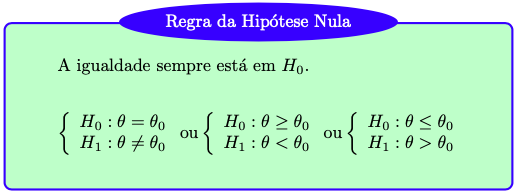
\includegraphics{img/regraH0.png}

As definições do quadro acima implicam em três tipos de hipótese alternativa, conforme figura a seguir. A hipótese \emph{bilateral} é a típica hipótese de equilíbrio, geralmente utilizada quando não há definição prévia sobre a direção da hipótese, tal como no caso de decidir se uma moeda deve ou não ser considerada equilibrada. A hipótese \emph{unilateral inferior} é uma hipótese que indica um piso de referência, tal como no caso de decidir sobre a eficácia mínima de um tratamento (maior, melhor). A hipótese \emph{unilateral superior} é uma hipótese que indica um teto de referência, tal como no caso de decidir sobre a uma ação dependente de uma taxa máxima de mortalidade (menor, melhor).

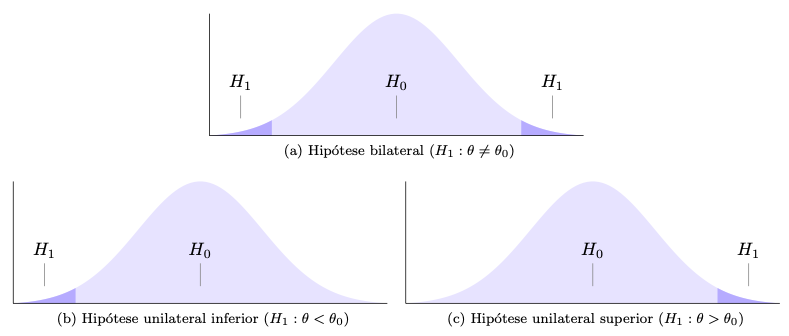
\includegraphics{img/regraH1.png}

\begin{exercise}
\protect\hypertarget{exr:hipoteses}{}{\label{exr:hipoteses} }Para cada item abaixo, indique as hipóteses sendo testadas.\\
\(\;\) \textbf{a.} A companhia de transporte afirma que, em média, o intervalo entre sucessivos ônibus de uma determinada linha é de 15 minutos. Uma associação de usuários de transportes coletivos acha que a pontualidade é muito importante, e deseja testar a afirmação da companhia.\\
\(\;\) \textbf{b.} Os amortecedores de automóveis que circulam em cidades duram pelo menos 100 mil quilômetros em média, segundo a informação de algumas oficinas especializadas. O proprietário de uma locadora de veículos deseja testar esta afirmação.\\
\(\;\) \textbf{c.} Um veterinário afirma ter obtido um ganho médio diário de pelo menos 3 litros de leite por vaca com uma nova composição de ração. Um pecuarista acredita que o ganho não é tão grande assim.\\
\(\;\) \textbf{d.} Algumas garrafas de cerveja declaram em seus rótulos conter 600mL. Os órgãos de fiscalização desejam avaliar se uma fábrica deve ou não ser autuada por engarrafar cervejas com uma quantidade menor que o indicado no rótulo.\\
\(\;\) \textbf{e.} O dado de um cassino parece estar viciado, saindo o valor 1 com uma frequência muito grande.\\
\(\;\) \textbf{f.} Um fabricante afirma que a sua vacina previne pelo menos 80\% dos casos de uma doença. Um grupo de médicos desconfia que a vacina não é tão eficiente assim. \(\\\)
\end{exercise}

A partir da premissa de que \(H_0\) é verdadeira, compara(m)-se o(s) valor(es) descrito(s) nesta hipótese com os dados da amostra através de uma medida chamada \emph{estatística de teste} ou \emph{quantidade pivotal}. Caso a estatística do teste indique uma pequena distância entre o(s) valor(es) de \(H_0\) e a estatística, \emph{admite-se} ou \emph{não se rejeita} \(H_0\); caso a distância seja grande, \emph{rejeita-se} \(H_0\). As distâncias que fazem admitir ou rejeitar \(H_0\) são avaliadas em termos probabilísticos, indicadas nos gráficos acima respectivamente pelas regiões claras e escuras. A divisão destas regiões é dada por \emph{valores críticos}, quantis das distribuições associadas às estatísticas de teste que serão detalhadas a seguir.

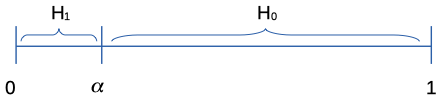
\includegraphics{img/decisao.png}

É possível ainda considerar formas mais precisas de avaliar as distâncias probabilisticas das estatísticas de teste do que simplesmente indicando `acima' ou `abaixo' de um valor crítico. Pelo paradigma clássico, atribui-se uma medida que varia entre 0 e 1, chamada \emph{p-value}, \emph{valor-p} ou \emph{nível descritivo amostral}. Este medida possui múltiplas definições e ainda é bastante discutida na literatura. Não é raro ser mal interpretada, portanto será considerada como um \emph{grau de evidência em favor de \(H_0\)}. Rejeita-se \(H_0\) se este grau de evidência for baixo, inferior a um valor de referência chamado \emph{nível de significância} e representado por \(\alpha\); caso contrário, admite-se ou não se rejeita \(H_0\). Este valor de significância está associado à probabilidade de \emph{erro do tipo I}, ou o caso em que erramos ao rejeitar uma hipótese \(H_0\) verdadeira. Tal valor é \emph{arbitrário}, ou seja, deve ser definido pelo dono do problema ao estipular o quanto admite de probabilidade máxima de erro do tipo I. Existem valores de significância típicos, usualmente 10\%, 5\%, 1\%, e 0.1\%. Devido a um exemplo dado por (Fisher \protect\hyperlink{ref-fisher1925statistical}{1925})\footnote{\emph{``The value for which P=.05, or 1 in 20, is 1.96 or nearly 2; it is convenient to take this point as a limit in judging whether a deviation is to be considered significant or not. Deviations exceeding twice the standard deviation are thus formally regarded as significant.''} Ronald Aylmer Fisher na primeira edição do seu livro \emph{Statistical Methods For Research Workers}, de 1925.}, o valor de 5\% tornou-se uma referência para o valor de \(\alpha\), ainda que existam propostas mais elaboradas e melhor embasadas na teoria Estatística. Destacam-se os trabalhos de (Gannon, Pereira, and Polpo \protect\hyperlink{ref-gannon2019blending}{2019}), (Pereira and Stern \protect\hyperlink{ref-pereira1999evidence}{1999}) e (Pereira and Wechsler \protect\hyperlink{ref-pereira1993concept}{1993}).

\hypertarget{associauxe7uxe3o-com-intervalos-de-confianuxe7a}{%
\subsubsection*{Associação com intervalos de confiança}\label{associauxe7uxe3o-com-intervalos-de-confianuxe7a}}
\addcontentsline{toc}{subsubsection}{Associação com intervalos de confiança}

Os testes de hipóteses possuem as mesmas características e propriedades dos seus respectivos intervalos de confiança. Desta forma, apresenta-se um breve exemplo abordando a equivalência entre os TH e os IC para a proporção universal \(\pi\).

\begin{example}
\protect\hypertarget{exm:equ-th-ic}{}{\label{exm:equ-th-ic} }(TH \(\equiv\) IC) Suponha uma moeda com probabilidade de face cara \(Pr(H)=\pi\). Em princípio não sabemos o valor de \(\pi\), e pode ser interessante considerar duas configurações:

\[\left\{ 
    \begin{array}{l}
      H_0: \mbox{a moeda é equilibrada}\\
      H_1: \mbox{a moeda não é equilibrada}\\ \end{array} \right.
    \equiv \left\{ 
    \begin{array}{l}
      H_0: \pi = 0.5 \\
      H_1: \pi \ne 0.5 \\ \end{array} \right. .\]

Sob \(H_{0}\) (i.e., supondo \(H_{0}\) verdadeira), espera-se observar `cara' em 50\% dos resultados, com alguma variação em torno de 50\%. Considerando a Equação \eqref{eq:ic-prop} pode-se obter a margem de erro esperada para esta oscilação em função do tamanho da amostra \(n\) para, digamos, 95\% dos casos: \[ IC \left[ \pi, 95\% \right] = 0.5 \mp 1.96 \sqrt{\dfrac{0.5 \left(1-0.5\right)}{n}} = 0.5 \mp \dfrac{0.98}{\sqrt{n}}. \]

Assim, ao realizar \(n=100\) lançamentos e observar uma frequência de caras no intervalo \[ IC \left[ \pi, 95\% \right]  = 0.5 \mp \dfrac{0.98}{\sqrt{100}} = \left[ 0.402,0.598 \right] = \left[ 40.2\%,59.8\% \right] \]

pode-se considerar a moeda equilibrada com \(1-\alpha=95\%\) de confiança. Caso a frequência seja inferior a \(40.2\%\) ou superior a \(59.8\%\), há indícios de que a moeda seja desequilibrada, também com 95\% de confiança. Pela terminologia dos testes de hipóteses, não se rejeita \(H_{0}\) com \(\alpha=5\%\).\\
Se \(n=25\), \[ IC \left[ \pi, 95\% \right]  = 0.5 \mp \dfrac{0.98}{\sqrt{25}} = \left[ 0.304,0.696 \right] = \left[ 30.4\%,69.6\% \right] \] e obtém-se um intervalo maior se comparado a \(n=100\), i.e., menos preciso para a mesma confiança de 95\%. Como exercício, use a função \texttt{ic} para definir outros valores para \(n\) e teste este resultado em uma moeda.
\end{example}

\begin{Shaded}
\begin{Highlighting}[]
\CommentTok{\# IC95\% sob H0: \textbackslash{}pi=0.5}
\NormalTok{ic \textless{}{-}}\StringTok{ }\ControlFlowTok{function}\NormalTok{(n)\{}
  \KeywordTok{cat}\NormalTok{(}\StringTok{\textquotesingle{}[\textquotesingle{}}\NormalTok{, }\FloatTok{0.5{-}.98}\OperatorTok{/}\KeywordTok{sqrt}\NormalTok{(n), }\StringTok{\textquotesingle{},\textquotesingle{}}\NormalTok{, }
           \FloatTok{0.5+.98}\OperatorTok{/}\KeywordTok{sqrt}\NormalTok{(n), }\StringTok{\textquotesingle{}]\textquotesingle{}}\NormalTok{)  }
\NormalTok{\}}
\KeywordTok{ic}\NormalTok{(}\DecValTok{100}\NormalTok{)}
\end{Highlighting}
\end{Shaded}

\begin{verbatim}
## [ 0.402 , 0.598 ]
\end{verbatim}

\begin{Shaded}
\begin{Highlighting}[]
\KeywordTok{ic}\NormalTok{(}\DecValTok{25}\NormalTok{)}
\end{Highlighting}
\end{Shaded}

\begin{verbatim}
## [ 0.304 , 0.696 ]
\end{verbatim}

\hypertarget{testes-paramuxe9tricos-univariados}{%
\subsection{Testes Paramétricos Univariados}\label{testes-paramuxe9tricos-univariados}}

\hypertarget{teste-1---teste-z-para-muxe9dia-de-uma-amostra}{%
\subsubsection*{\texorpdfstring{TESTE 1 - Teste \(z\) para média de uma amostra}{TESTE 1 - Teste z para média de uma amostra}}\label{teste-1---teste-z-para-muxe9dia-de-uma-amostra}}
\addcontentsline{toc}{subsubsection}{TESTE 1 - Teste \(z\) para média de uma amostra}

\textbf{Hipótese avaliada}\\
Uma amostra de \(n\) sujeitos (ou objetos) vem de uma população de média \(\mu\) igual a um valor especificado \(\mu_0\)?

\textbf{Suposições}\\
S1. O desvio padrão universal \(\sigma\) é conhecido;\\
S2. A amostra foi selecionada aleatoriamente da população que representa;\\
S3. A distribuição dos dados na população que a amostra representa é normal. Pelo Teorema Central do Limite, tal suposição torna-se menos importante à medida que o tamanho da amostra aumenta.

\textbf{Testes relacionados}\\
TESTE 13 - Teste dos postos sinalizados de Wilcoxon para uma amostra

\textbf{Estatística do teste}\\
Sob \(H_0: \mu = \mu_0\), \(H_0: \mu \ge \mu_0\) ou \(H_0: \mu \le \mu_0\),
\begin{equation}
z_{teste}=\frac{\bar{x}-\mu_0}{\sigma/\sqrt{n}} \sim \mathcal{N}(0,1).
\label{eq:z-teste-media-uni}
\end{equation}

\textbf{Valor-p}\\
Sob \(H_0: \mu = \mu_0\),
\begin{equation}
\text{Valor-p} = 2Pr(Z \le -|z_{teste}|).
\label{eq:z-teste-media-uni-p-bi}
\end{equation}

Sob \(H_0: \mu \ge \mu_0\),
\begin{equation}
\text{Valor-p} = Pr(Z \le z_{teste}).
\label{eq:z-teste-media-uni-p-uni-inf}
\end{equation}

Sob \(H_0: \mu \le \mu_0\),
\begin{equation}
\text{Valor-p} = Pr(Z \ge z_{teste}).
\label{eq:z-teste-media-uni-p-uni-sup}
\end{equation}

\begin{example}
\protect\hypertarget{exm:z-teste}{}{\label{exm:z-teste} }É desejado testar se a média de altura dos alunos da PUCRS pode ser considerada \emph{maior} do que 167 cm. A hipótese é portanto unilateral superior na forma \(H_0: \mu \le 167\) \emph{vs} \(H_1: \mu > 167\). Estudos anteriores indicam que a variável \(X\): `altura dos alunos da PUCRS' tem distribuição normal de média desconhecida (motivo da realização do teste de hipóteses para \(\mu\)) e desvio padrão \(\sigma=14\), indicado por \(X \sim \mathcal{N}(\mu,14)\). De uma amostra aleatória com \(n=25\) pessoas obteve-se \(\bar{x}_{25}=172\). Assim, sob \(H_0\) a estatística do teste pode ser calculada da seguinte maneira:
\[z_{teste} = \frac{172-167}{14/\sqrt{25}} \approx 1.786 \approx 1.79.\]
Se utilizarmos \(\alpha=0.05\) (unilateral superior), \(z_{cr\acute{\imath}tico}=1.64\). Como a estatística de teste extrapola o valor crítico, i.e., \(1.79 > 1.64\), rejeita-se \(H_0\). \(\\\)\\
\emph{Decisão Estatística}: Rejeita-se \(H_0\) com \(\alpha=5\%\) pois \(1.79 > 1.64\).\\
\emph{Conclusão Experimental}: A amostra sugere que a média de altura dos alunos da PUCRS deve ser maior do que 167 cm. \(\\\)
\end{example}

\begin{example}
\protect\hypertarget{exm:z-teste-pvalue}{}{\label{exm:z-teste-pvalue} }No Exemplo \ref{exm:z-teste} é possível calcular o valor p associado à estatística de teste \(z_{teste} \approx 1.79\). Por ser um teste unilateral superior, basta obter a probabilidade de encontrar um valor tão ou mais extremo que \(z_{teste}\) conforme Equação \eqref{eq:z-teste-media-uni-p-uni-inf}. Pela tabela de normal padrão (com precisão inferior à do computador) \[\text{Valor-p} = Pr(Z \ge 1.79) = 1-Pr(Z<1.79) = 1-0.9633 = 0.0367.\] Utilizando \(\alpha=0.05\) unilateral decide-se novamente pela rejeição de \(H_0\) uma vez que o valor p é inferior ao nível de significância, i.e., \(0.0367 < 0.05\). A decisão realizada desta maneira deve sempre ser a mesma quando compara-se a estatística do teste com o(s) valor(es) crítico(s). \(\\\)\\
\emph{Decisão Estatística}: Rejeita-se \(H_0\) com \(\alpha=5\%\) pois \(0.0367 < 0.05\).\\
\emph{Conclusão Experimental}: A amostra sugere que a média de altura dos alunos da PUCRS deve ser maior do que 167 cm. \(\\\)
\end{example}

\begin{example}
\protect\hypertarget{exm:z-teste-r}{}{\label{exm:z-teste-r} }Realizando os Exemplos \ref{exm:z-teste} e \ref{exm:z-teste-pvalue} no R.
\end{example}

\begin{Shaded}
\begin{Highlighting}[]
\CommentTok{\# Definindo os valores indicados no enunciado}
\NormalTok{mu0 \textless{}{-}}\StringTok{ }\DecValTok{167}
\NormalTok{n \textless{}{-}}\StringTok{ }\DecValTok{25}
\NormalTok{x\_bar \textless{}{-}}\StringTok{ }\DecValTok{172}
\NormalTok{sigma \textless{}{-}}\StringTok{ }\DecValTok{14}
\NormalTok{(zt \textless{}{-}}\StringTok{ }\NormalTok{(x\_bar}\OperatorTok{{-}}\NormalTok{mu0)}\OperatorTok{/}\NormalTok{(sigma}\OperatorTok{/}\KeywordTok{sqrt}\NormalTok{(n))) }\CommentTok{\# estatística do teste, note a maior precisão}
\end{Highlighting}
\end{Shaded}

\begin{verbatim}
## [1] 1.79
\end{verbatim}

\begin{Shaded}
\begin{Highlighting}[]
\KeywordTok{curve}\NormalTok{(}\KeywordTok{dnorm}\NormalTok{(x), }\DecValTok{{-}3}\NormalTok{, }\DecValTok{3}\NormalTok{) }\CommentTok{\# gráfico da normal padrão}
\KeywordTok{abline}\NormalTok{(}\DataTypeTok{v =} \KeywordTok{qnorm}\NormalTok{(.}\DecValTok{95}\NormalTok{), }\DataTypeTok{col =} \StringTok{\textquotesingle{}red\textquotesingle{}}\NormalTok{) }\CommentTok{\# valor crítico de ≈1.64}
\end{Highlighting}
\end{Shaded}

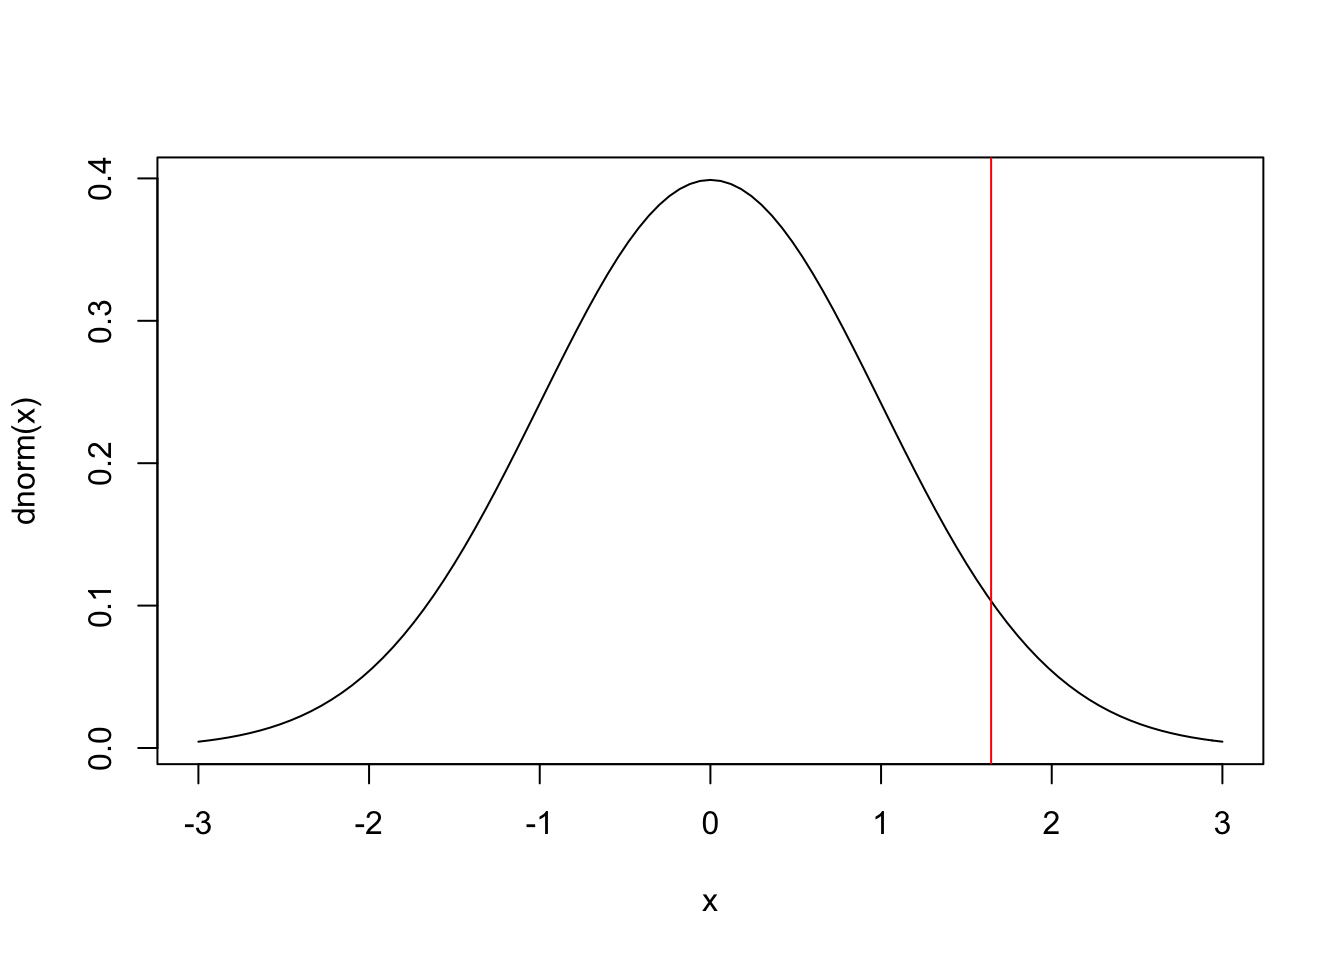
\includegraphics{_main_files/figure-latex/unnamed-chunk-94-1.pdf}

\begin{Shaded}
\begin{Highlighting}[]
\DecValTok{1}\OperatorTok{{-}}\KeywordTok{pnorm}\NormalTok{(zt) }\CommentTok{\# p{-}value mais preciso por conta de zt e pnorm}
\end{Highlighting}
\end{Shaded}

\begin{verbatim}
## [1] 0.0371
\end{verbatim}

\hypertarget{teste-2---teste-t-para-muxe9dia-de-uma-amostra}{%
\subsubsection*{\texorpdfstring{TESTE 2 - Teste \(t\) para média de uma amostra}{TESTE 2 - Teste t para média de uma amostra}}\label{teste-2---teste-t-para-muxe9dia-de-uma-amostra}}
\addcontentsline{toc}{subsubsection}{TESTE 2 - Teste \(t\) para média de uma amostra}

\textbf{Hipótese avaliada}\\
Uma amostra de \(n\) sujeitos (ou objetos) vem de uma população de média \(\mu\) igual a um valor especificado \(\mu_0\)?

\textbf{Suposições}\\
S1. A amostra foi selecionada aleatoriamente da população que representa;\\
S2. A distribuição dos dados na população que a amostra representa é normal.

\textbf{Testes relacionados}\\
TESTE 14 - Teste dos postos sinalizados de Wilcoxon para uma amostra

\textbf{Estatística do teste}\\
Sob \(H_0: \mu = \mu_0\),
\begin{equation}
t_{teste}=\frac{\bar{x}-\mu_0}{s/\sqrt{n}} \sim \mathcal{t}(gl),
\label{eq:t-teste-media-uni}
\end{equation}

onde \(gl=n-1\) indica os \emph{graus de liberdade} que definem a distribuição \(t\).

\textbf{Valor-p}\\
Sob \(H_0: \mu = \mu_0\),
\begin{equation}
\text{Valor-p} = 2Pr(T \le -|t_{teste}|).
\label{eq:t-teste-media-uni-p-bi}
\end{equation}

Sob \(H_0: \mu \ge \mu_0\),
\begin{equation}
\text{Valor-p} = Pr(T \le t_{teste}).
\label{eq:t-teste-media-uni-p-uni-inf}
\end{equation}

Sob \(H_0: \mu \le \mu_0\),
\begin{equation}
\text{Valor-p} = Pr(T \ge t_{teste}).
\label{eq:t-teste-media-uni-p-uni-sup}
\end{equation}

\begin{example}
\protect\hypertarget{exm:t-teste}{}{\label{exm:t-teste} }É desejado testar se a média de altura dos alunos da PUCRS pode ser considerada \emph{maior} do que 167 cm. A hipótese é portanto unilateral superior na forma \(H_0: \mu \le 167\) \emph{vs} \(H_1: \mu > 167\). Estudos anteriores indicam que a variável \(X\): `altura dos alunos da PUCRS' tem distribuição normal de média e desvio padrão desconhecidos, indicado por \(X \sim \mathcal{N}(\mu,\sigma)\). De uma amostra aleatória com \(n=25\) pessoas obteve-se \(\bar{x}_{25}=172\) e \(s_{25}=14\). Assim, sob \(H_0\) a estatística do teste pode ser calculada da seguinte maneira:
\[t_{teste} = \frac{172-167}{14/\sqrt{25}} \approx 1.786.\]
Se utilizarmos \(\alpha=0.05\) (unilateral superior), \(t_{cr\acute{\imath}tico}=1.711\), considerando \(gl=24\) graus de liberdade. Como a estatística de teste extrapola o valor crítico, i.e., \(1.786 > 1.711\), rejeita-se \(H_0\). \(\\\)\\
\emph{Decisão Estatística}: Rejeita-se \(H_0\) com \(\alpha=5\%\) pois \(1.786 > 1.711\).\\
\emph{Conclusão Experimental}: A amostra sugere que a média de altura dos alunos da PUCRS deve ser maior do que 167 cm. \(\\\)
\end{example}

\begin{example}
\protect\hypertarget{exm:t-teste-pvalue}{}{\label{exm:t-teste-pvalue} }No Exemplo \ref{exm:t-teste} é possível obter um intervalo para o valor p associado à estatística de teste \(t_{teste} \approx 1.786\). Por ser um teste unilateral superior, deve-se obter a probabilidade de encontrar um valor tão ou mais extremo que \(t_{teste}\) conforme Equação \eqref{eq:t-teste-media-uni-p-uni-inf}. Pela tabela de \(t\) com \(gl=24\) graus de liberdade obtém-se \(Pr(t>1.711) = 0.05\) e \(Pr(t>2.064) = 0.025\). Dada a limitação de precisão da tabela \(t\), pode-se apenas concluir que \(0.025 < Pr(t>1.786) < 0.05\). Utilizando \(\alpha=0.05\) unilateral decide-se novamente pela rejeição de \(H_0\) uma vez que o valor p é inferior ao nível de significância, i.e., \(Pr(t>1.786) < 0.05\). A decisão realizada desta maneira deve sempre ser a mesma quando compara-se a estatística do teste com o(s) valor(es) crítico(s). \(\\\)\\
\emph{Decisão Estatística}: Rejeita-se \(H_0\) com \(\alpha=5\%\) pois \(Pr(t>1.786) < 0.05\).\\
\emph{Conclusão Experimental}: A amostra sugere que a média de altura dos alunos da PUCRS deve ser maior do que 167 cm. \(\\\)
\end{example}

\begin{example}
\protect\hypertarget{exm:t-teste-r}{}{\label{exm:t-teste-r} }Realizando os Exemplos \ref{exm:t-teste} e \ref{exm:t-teste-pvalue} no R.
\end{example}

\begin{Shaded}
\begin{Highlighting}[]
\CommentTok{\# Definindo os valores indicados no enunciado}
\NormalTok{mu0 \textless{}{-}}\StringTok{ }\DecValTok{167}
\NormalTok{n \textless{}{-}}\StringTok{ }\DecValTok{25}
\NormalTok{x\_bar \textless{}{-}}\StringTok{ }\DecValTok{172}
\NormalTok{s \textless{}{-}}\StringTok{ }\DecValTok{14}
\NormalTok{(tt \textless{}{-}}\StringTok{ }\NormalTok{(x\_bar}\OperatorTok{{-}}\NormalTok{mu0)}\OperatorTok{/}\NormalTok{(s}\OperatorTok{/}\KeywordTok{sqrt}\NormalTok{(n))) }\CommentTok{\# estatística do teste, note a maior precisão}
\end{Highlighting}
\end{Shaded}

\begin{verbatim}
## [1] 1.79
\end{verbatim}

\begin{Shaded}
\begin{Highlighting}[]
\KeywordTok{curve}\NormalTok{(}\KeywordTok{dt}\NormalTok{(x, }\DataTypeTok{df =}\NormalTok{ n}\DecValTok{{-}1}\NormalTok{), }\DecValTok{{-}3}\NormalTok{, }\DecValTok{3}\NormalTok{) }\CommentTok{\# gráfico da t com gl=25{-}1=24}
\KeywordTok{abline}\NormalTok{(}\DataTypeTok{v =} \KeywordTok{qt}\NormalTok{(.}\DecValTok{95}\NormalTok{, }\DataTypeTok{df =}\NormalTok{ n}\DecValTok{{-}1}\NormalTok{), }\DataTypeTok{col =} \StringTok{\textquotesingle{}red\textquotesingle{}}\NormalTok{) }\CommentTok{\# valor crítico de ≈1.711}
\end{Highlighting}
\end{Shaded}

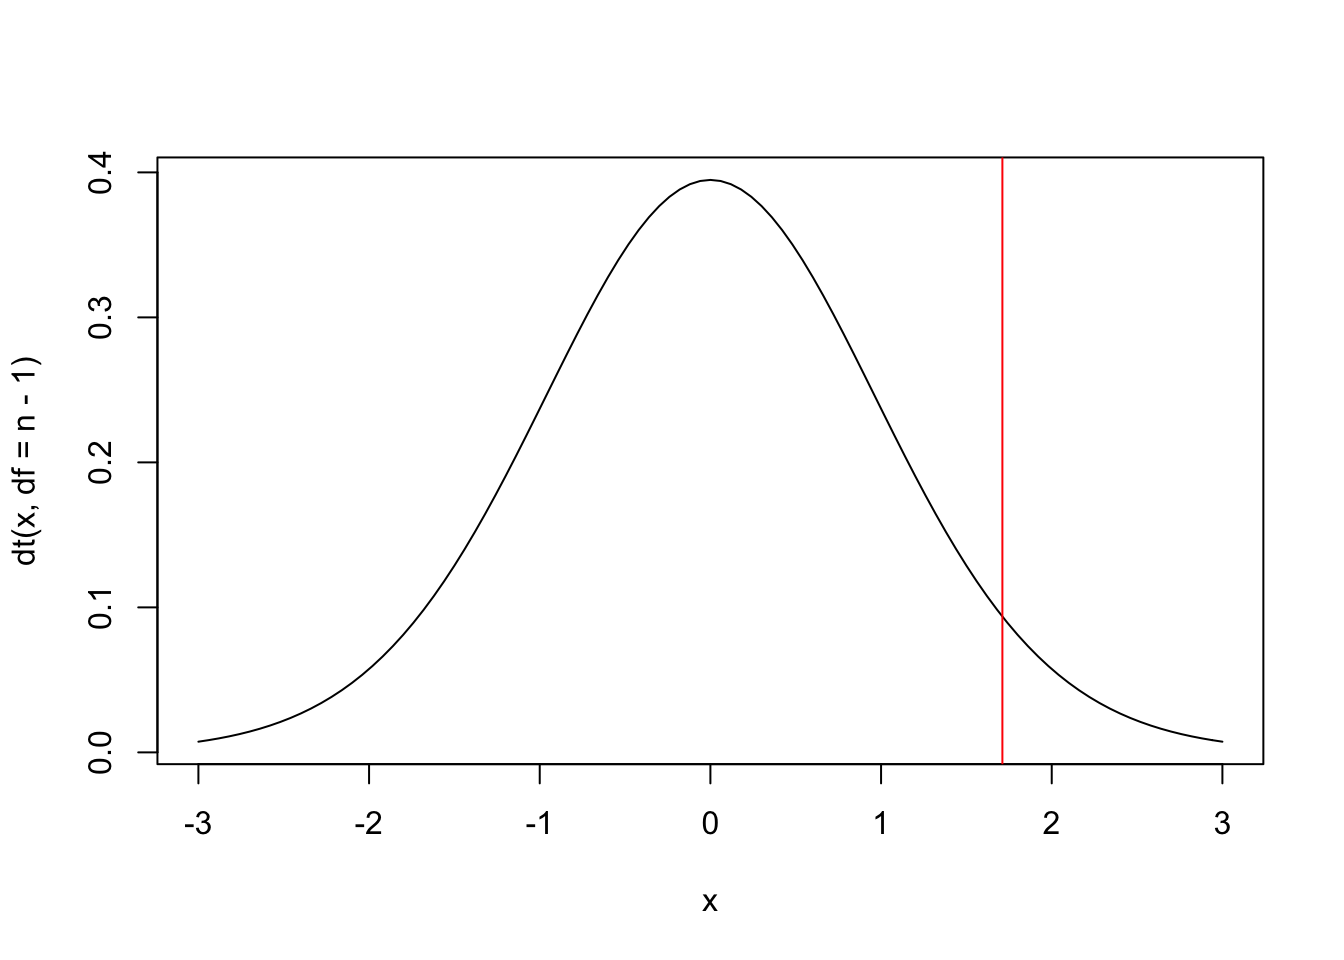
\includegraphics{_main_files/figure-latex/unnamed-chunk-95-1.pdf}

\begin{Shaded}
\begin{Highlighting}[]
\DecValTok{1}\OperatorTok{{-}}\KeywordTok{pt}\NormalTok{(tt, }\DataTypeTok{df =}\NormalTok{ n}\DecValTok{{-}1}\NormalTok{) }\CommentTok{\# p{-}value mais preciso por conta de tt e pt}
\end{Highlighting}
\end{Shaded}

\begin{verbatim}
## [1] 0.0434
\end{verbatim}

\hypertarget{teste-3---testes-para-proporuxe7uxe3o-de-uma-amostra-binomial-exato-e-normal-assintuxf3tico}{%
\subsubsection*{TESTE 3 - Testes para proporção de uma amostra, binomial (exato) e normal (assintótico)}\label{teste-3---testes-para-proporuxe7uxe3o-de-uma-amostra-binomial-exato-e-normal-assintuxf3tico}}
\addcontentsline{toc}{subsubsection}{TESTE 3 - Testes para proporção de uma amostra, binomial (exato) e normal (assintótico)}

\textbf{Hipótese avaliada}\\
Em uma população composta de duas categorias, a proporção \(\pi\) de observações em uma das categorias é igual a um valor específico \(\pi_0\)?

\textbf{Suposições}\\
S1. Cada observação pode ser classificada em \emph{sucesso} ou \emph{fracasso};\\
S2. Cada uma das \(n\) observações (condicionalmente) independentes é selecionada aleatoriamente de uma população;\\
S3. A probabilidade de sucesso \(\pi\) se mantém constante a cada observação.

\textbf{Estatística do teste (assintótico)}\\
Sob \(H_0: \pi = \pi_0\),
\begin{equation}
z_{teste}=\frac{p-\pi_0}{\sqrt{\pi_0 (1-\pi_0)/n}} \sim \mathcal{N}(0,1).
\label{eq:z-teste-prop-uni}
\end{equation}

\textbf{Valor-p (assintótico)}\\
Sob \(H_0: \pi = \pi_0\), vide Equação \eqref{eq:z-teste-media-uni-p-bi}.

Sob \(H_0: \pi \ge \pi_0\), vide Equação \eqref{eq:z-teste-media-uni-p-uni-inf}.

Sob \(H_0: \pi \le \pi_0\), vide Equação \eqref{eq:z-teste-media-uni-p-uni-sup}.

\textbf{Valor-p (exato)}\\
Seja \(X\) o número de sucessos em \(n\) ensaios de Bernoulli. Sob \(H_0: \pi = \pi_0\) ocorre que \(X \sim \mathcal{B}(n,\pi_0)\), se \(x>\frac{n}{2}\) e \(I = \{ 0,1,\ldots,n-x, x,\ldots,n \}\),
\begin{equation}
\text{Valor-p} = Pr(n-x \ge X \ge x | \pi = \pi_0) = \sum_{i \in I} {n \choose i} \pi_{0}^i (1-\pi_0)^{n-i},
\label{eq:binom-prop-uni-sup-xmaior}
\end{equation}

se \(x<\frac{n}{2}\) e \(I = \{ 0,1,\ldots,x, n-x,\ldots,n \}\),
\begin{equation}
\text{Valor-p} = Pr(x \ge X \ge n-x | \pi = \pi_0) = \sum_{i \in I} {n \choose i} \pi_{0}^i (1-\pi_0)^{n-i},
\label{eq:binom-prop-uni-sup-xmenor}
\end{equation}

e \(\text{Valor-p} = 1\) se \(x=\frac{n}{2}\).

Sob \(H_0: \pi \le \pi_0\),
\begin{equation}
\text{Valor-p} = Pr(X \ge x | \pi = \pi_0) = \sum_{i=x}^{n} {n \choose i} \pi_{0}^i (1-\pi_0)^{n-i}
\label{eq:binom-prop-uni-sup}
\end{equation}

Sob \(H_0: \pi \ge \pi_0\),
\begin{equation}
\text{Valor-p} = Pr(X \le x | \pi = \pi_0) = \sum_{i=0}^{x} {n \choose i} \pi_{0}^i (1-\pi_0)^{n-i}
\label{eq:binom-prop-uni-inf}
\end{equation}

\begin{example}
\protect\hypertarget{exm:prop-uni-sup-assint}{}{\label{exm:prop-uni-sup-assint} }Suponha que deseja-se testar \(\pi\), a proporção de caras em uma moeda, na forma \(H_0: \pi \le 0.5\) \emph{vs} \(H_1 : \pi > 0.5\). Para isso a moeda é lançada \(n=12\) vezes, onde se observam \(x=9\) caras e \(n-x=12-9=3\) coroas. Sabe-se que \(p=\frac{9}{12}=\frac{3}{4}=0.75\). Considerando a abordagem assintótica, sob \(H_0\) \[z_{teste}=\frac{0.75-0.5}{\sqrt{0.5 (1-0.5)/12}} \approx 1.73.\] Se utilizarmos \(\alpha=0.05\) (unilateral superior), \(z_{cr\acute{\imath}tico}=1.64\). Como a estatística de teste extrapola o valor crítico, i.e., \(1.73 > 1.64\), rejeita-se \(H_0\). \(\\\)\\
\emph{Decisão Estatística}: Rejeita-se \(H_0\) com \(\alpha=5\%\) pois \(1.73 > 1.64\).\\
\emph{Conclusão Experimental}: A amostra sugere que a proporção de caras da moeda deve ser considerada maior que 0.5. \(\\\)\\
\end{example}

\begin{example}
\protect\hypertarget{exm:prop-uni-sup-assint-pvalue}{}{\label{exm:prop-uni-sup-assint-pvalue} }Considere novamente os dados do Exemplo \ref{exm:prop-uni-sup-assint}. Pela Equação \eqref{eq:z-teste-media-uni-p-uni-sup} utilizando a tabela de normal padrão (com precisão inferior à do computador), \[\text{Valor-p} = Pr(Z \ge 1.73) = 1-Pr(Z<1.73) = 1-0.9582 = 0.0418.\] Utilizando \(\alpha=0.05\) unilateral decide-se novamente pela rejeição de \(H_0\) uma vez que o valor p é inferior ao nível de significância, i.e., \(0.0418 < 0.05\). A decisão realizada desta maneira deve sempre ser a mesma quando compara-se a estatística do teste com o(s) valor(es) crítico(s). \(\\\)\\
\emph{Decisão Estatística}: Rejeita-se \(H_0\) com \(\alpha=5\%\) pois \(0.0418 < 0.05\).\\
\emph{Conclusão Experimental}: A amostra sugere que a proporção de caras da moeda deve ser considerada maior que 0.5. \(\\\)
\end{example}

\begin{example}
\protect\hypertarget{exm:prop-teste-assint-r}{}{\label{exm:prop-teste-assint-r} }Realizando os Exemplos \ref{exm:prop-uni-sup-assint} e \ref{exm:prop-uni-sup-assint-pvalue} no R.
\end{example}

\begin{Shaded}
\begin{Highlighting}[]
\NormalTok{n \textless{}{-}}\StringTok{ }\DecValTok{12}
\NormalTok{x \textless{}{-}}\StringTok{ }\DecValTok{9}
\NormalTok{(p \textless{}{-}}\StringTok{ }\NormalTok{x}\OperatorTok{/}\NormalTok{n)}
\end{Highlighting}
\end{Shaded}

\begin{verbatim}
## [1] 0.75
\end{verbatim}

\begin{Shaded}
\begin{Highlighting}[]
\NormalTok{pi0 \textless{}{-}}\StringTok{ }\FloatTok{0.5}
\NormalTok{(zt \textless{}{-}}\StringTok{ }\NormalTok{(p}\OperatorTok{{-}}\NormalTok{pi0)}\OperatorTok{/}\KeywordTok{sqrt}\NormalTok{(pi0}\OperatorTok{*}\NormalTok{(}\DecValTok{1}\OperatorTok{{-}}\NormalTok{pi0)}\OperatorTok{/}\NormalTok{n))}
\end{Highlighting}
\end{Shaded}

\begin{verbatim}
## [1] 1.73
\end{verbatim}

\begin{Shaded}
\begin{Highlighting}[]
\DecValTok{1}\OperatorTok{{-}}\KeywordTok{pnorm}\NormalTok{(zt) }\CommentTok{\# p{-}value mais preciso por conta de zt e pnorm}
\end{Highlighting}
\end{Shaded}

\begin{verbatim}
## [1] 0.0416
\end{verbatim}

\begin{Shaded}
\begin{Highlighting}[]
\CommentTok{\# usando a função prop.test, sem a correção de Yates}
\KeywordTok{prop.test}\NormalTok{(x, n, pi0, }\DataTypeTok{alternative =} \StringTok{\textquotesingle{}greater\textquotesingle{}}\NormalTok{, }\DataTypeTok{correct =} \OtherTok{FALSE}\NormalTok{)}
\end{Highlighting}
\end{Shaded}

\begin{verbatim}
## 
##  1-sample proportions test without continuity correction
## 
## data:  x out of n, null probability pi0
## X-squared = 3, df = 1, p-value = 0.04
## alternative hypothesis: true p is greater than 0.5
## 95 percent confidence interval:
##  0.513 1.000
## sample estimates:
##    p 
## 0.75
\end{verbatim}

\begin{example}
\protect\hypertarget{exm:prop-uni-sup-exato}{}{\label{exm:prop-uni-sup-exato} }Considere novamente os dados do Exemplo \ref{exm:prop-uni-sup-assint}. O teste exato pode ser realizado considerando que sob \(H_0: \pi \le 0.5\), o número de caras (sucessos) \(X\) tem distribuição binomial de parâmetros \(n=12\) e \(\pi=0.5\), i.e., \(X \sim \mathcal{B}(12,0.5)\). Assim, o valor-p exato resulta em
\begin{equation}
Pr\left( X \geq 9 | \pi = 0.5 \right) = \left[ \binom {12}{9} + \binom {12}{10} + \binom {12}{11} + \binom {12}{12} \right] \times 0.5^{12} \approx 0.0730. \nonumber
\end{equation}
Note a diferença do valor exato em comparação ao assintótico.\\
\emph{Decisão Estatística}: não se rejeita \(H_0\) com \(\alpha=5\%\) pois \(0.0730 > 0.05\).\\
\emph{Conclusão Experimental}: a amostra sugere que a proporção de caras da moeda pode ser considerada menor ou igual a 0.5. \(\\\)
\end{example}

\begin{example}
\protect\hypertarget{exm:prop-teste-exato-r}{}{\label{exm:prop-teste-exato-r} }Realizando o Exemplo \ref{exm:prop-uni-sup-exato} no R.
\end{example}

\begin{Shaded}
\begin{Highlighting}[]
\CommentTok{\# manualmente}
\NormalTok{n \textless{}{-}}\StringTok{ }\DecValTok{12}
\NormalTok{x \textless{}{-}}\StringTok{ }\DecValTok{9}
\NormalTok{pi0 \textless{}{-}}\StringTok{ }\FloatTok{0.5}
\NormalTok{p9 \textless{}{-}}\StringTok{ }\KeywordTok{dbinom}\NormalTok{(}\DecValTok{9}\NormalTok{,n,pi0)}
\NormalTok{p10 \textless{}{-}}\StringTok{ }\KeywordTok{dbinom}\NormalTok{(}\DecValTok{10}\NormalTok{,n,pi0)}
\NormalTok{p11 \textless{}{-}}\StringTok{ }\KeywordTok{dbinom}\NormalTok{(}\DecValTok{11}\NormalTok{,n,pi0)}
\NormalTok{p12 \textless{}{-}}\StringTok{ }\KeywordTok{dbinom}\NormalTok{(}\DecValTok{12}\NormalTok{,n,pi0)}
\NormalTok{p9}\OperatorTok{+}\NormalTok{p10}\OperatorTok{+}\NormalTok{p11}\OperatorTok{+}\NormalTok{p12 }\CommentTok{\# valor{-}p}
\end{Highlighting}
\end{Shaded}

\begin{verbatim}
## [1] 0.073
\end{verbatim}

\begin{Shaded}
\begin{Highlighting}[]
\CommentTok{\# usando a função binom.test}
\KeywordTok{binom.test}\NormalTok{(x, n, pi0, }\DataTypeTok{alternative =} \StringTok{\textquotesingle{}greater\textquotesingle{}}\NormalTok{)}
\end{Highlighting}
\end{Shaded}

\begin{verbatim}
## 
##  Exact binomial test
## 
## data:  x and n
## number of successes = 9, number of trials = 12, p-value = 0.07
## alternative hypothesis: true probability of success is greater than 0.5
## 95 percent confidence interval:
##  0.473 1.000
## sample estimates:
## probability of success 
##                   0.75
\end{verbatim}

\begin{Shaded}
\begin{Highlighting}[]
\CommentTok{\# usando a função prop.test (assintótico mas com correção de continuidade de Yates)}
\KeywordTok{prop.test}\NormalTok{(x, n, pi0, }\DataTypeTok{alternative =} \StringTok{\textquotesingle{}greater\textquotesingle{}}\NormalTok{)}
\end{Highlighting}
\end{Shaded}

\begin{verbatim}
## 
##  1-sample proportions test with continuity correction
## 
## data:  x out of n, null probability pi0
## X-squared = 2, df = 1, p-value = 0.07
## alternative hypothesis: true p is greater than 0.5
## 95 percent confidence interval:
##  0.471 1.000
## sample estimates:
##    p 
## 0.75
\end{verbatim}

\begin{exercise}
\protect\hypertarget{exr:prop-bi}{}{\label{exr:prop-bi} }Refaça os Exemplos \ref{exm:prop-uni-sup-assint}, \ref{exm:prop-uni-sup-assint-pvalue} e \ref{exm:prop-uni-sup-exato} considerando \(H_0: \pi = 0.6\) \emph{vs} \(H_1 : \pi \ne 0.6\). \(\\\)
\end{exercise}

\begin{exercise}
\protect\hypertarget{exr:prop-hotel}{}{\label{exr:prop-hotel} }Uma rádio do estado anunciou que 90\% dos hotéis da Serra Gaúcha estariam lotados no final de semana do dia dos pais. A estação aconselhou os ouvintes a fazerem reserva antecipada para se hospedar na Serra nestes dias. No sábado à noite uma amostra de 58 hotéis revelou que 49 diziam `sem vagas'. Qual é a sua reação à afirmação da rádio, depois de ver a evidência da amostra? Use 5\% de nível de significância. \(\\\)
\end{exercise}

\begin{exercise}
\protect\hypertarget{exr:prop-pecas}{}{\label{exr:prop-pecas} }Você é responsável por avaliar a qualidade de um grande lote de peças de segunda mão adquiridas pela sua empresa. O fabricante afirma haver no máximo 10\% de peças defeituosas, e você decide investigar. Para isso você retira uma amostra de 50 peças, das quais 9 são defeituosas. Qual a sua opinião sobre o lote adquirido, considerando níveis de significância de 1\%, 5\% e 10\%? Defina as hipóteses, apresentando a Decisão Estatística e a Conclusão Experimental. \(\\\)
\end{exercise}

\hypertarget{teste-4---teste-qui-quadrado-para-a-variuxe2ncia-populacional-de-uma-amostra}{%
\subsubsection*{TESTE 4 - Teste qui-quadrado para a variância populacional de uma amostra}\label{teste-4---teste-qui-quadrado-para-a-variuxe2ncia-populacional-de-uma-amostra}}
\addcontentsline{toc}{subsubsection}{TESTE 4 - Teste qui-quadrado para a variância populacional de uma amostra}

\textbf{Hipótese avaliada}\\
Uma amostra de \(n\) sujeitos (ou objetos) vem de uma população na qual a variância \(\sigma^2\) é igual a um valor especificado \(\sigma_0^2\)?

\textbf{Suposições}\\
S1. A amostra foi selecionada aleatoriamente da população que representa;\\
S2. A distribuição dos dados na população que a amostra representa é normal.

\textbf{Estatística do teste}\\
Sob \(H_0: \sigma^2 = \sigma_0^2\),
\begin{equation}
\chi_{teste}^2=\frac{(n-1)s^2}{\sigma_0^2} \sim \mathcal{\chi}^2(gl),
\label{eq:qui-teste-var-uni}
\end{equation}

onde \(gl=n-1\) indica os \emph{graus de liberdade} que definem a distribuição \(\chi^2\).

\textbf{Valor-p}\\
Sob \(H_0: \sigma^2 = \sigma_0^2\),
\begin{equation}
\text{Valor-p} = 2Pr(\chi^2 \le \chi_{teste}^2).
\label{eq:qui-teste-var-uni-p-bi}
\end{equation}

Sob \(H_0: \sigma^2 \ge \sigma_0^2\),
\begin{equation}
\text{Valor-p} = Pr(\chi^2 \le \chi_{teste}^2).
\label{eq:qui-teste-var-uni-p-uni-inf}
\end{equation}

Sob \(H_0: \sigma^2 \le \sigma_0^2\),
\begin{equation}
\text{Valor-p} = Pr(\chi^2 \ge \chi_{teste}^2).
\label{eq:qui-teste-var-uni-p-uni-sup}
\end{equation}

\begin{example}
\protect\hypertarget{exm:qui-var}{}{\label{exm:qui-var} }Deseja-se testar se a variância de uma variável com distribuição normal pode ser considerada igual a 5, i.e., \(H_0: \sigma^2 = 5\) \emph{vs} \(H_0: \sigma^2 \ne 5\). Para isso observa-se uma amostra de tamanho \(n=41\), de onde se calcula uma variância amostral de \(s^2 \approx 3.196876\). Sob \(H_0\) \[\chi_{teste}^2=\frac{(41-1) \times 3.196876 }{5} \approx 25.58.\] Considerando \(\alpha=0.05\) (bilateral) e a tabela qui-quadrado com \(gl=41-1=40\), \(\chi_{cr\acute{\imath}tico1}^2=24.43\) e \(\chi_{cr\acute{\imath}tico2}^2=59.34\). Como a estatística de teste não extrapola os valores críticos, i.e., \(24.43 < 25.58 < 59.34\), não se rejeita \(H_0\). \(\\\)\\
\emph{Decisão Estatística}: Não se rejeita \(H_0\) com \(\alpha=0.05\) pois \(24.43 < 25.58 < 59.34\).\\
\emph{Conclusão Experimental}: A amostra sugere que a variância da referida variável pode ser considerada igual a 5. \(\\\)
\end{example}

\begin{example}
\protect\hypertarget{exm:qui-var-r}{}{\label{exm:qui-var-r} }Realizando o Exemplo \ref{exm:qui-var} no R.
\end{example}

\begin{Shaded}
\begin{Highlighting}[]
\CommentTok{\# Definindo os valores indicados no enunciado}
\NormalTok{sigma2\_}\DecValTok{0}\NormalTok{ \textless{}{-}}\StringTok{ }\DecValTok{5}
\NormalTok{n \textless{}{-}}\StringTok{ }\DecValTok{41}
\KeywordTok{set.seed}\NormalTok{(}\DecValTok{123}\NormalTok{); x \textless{}{-}}\StringTok{ }\KeywordTok{rnorm}\NormalTok{(n, }\DataTypeTok{mean =} \DecValTok{0}\NormalTok{, }\DataTypeTok{sd =} \DecValTok{2}\NormalTok{)}
\NormalTok{(s2 \textless{}{-}}\StringTok{ }\KeywordTok{var}\NormalTok{(x))}
\end{Highlighting}
\end{Shaded}

\begin{verbatim}
## [1] 3.2
\end{verbatim}

\begin{Shaded}
\begin{Highlighting}[]
\NormalTok{(quit \textless{}{-}}\StringTok{ }\NormalTok{((n}\DecValTok{{-}1}\NormalTok{)}\OperatorTok{*}\NormalTok{s2)}\OperatorTok{/}\NormalTok{sigma2\_}\DecValTok{0}\NormalTok{) }\CommentTok{\# estatística do teste, note a maior precisão}
\end{Highlighting}
\end{Shaded}

\begin{verbatim}
## [1] 25.6
\end{verbatim}

\begin{Shaded}
\begin{Highlighting}[]
\KeywordTok{curve}\NormalTok{(}\KeywordTok{dchisq}\NormalTok{(x, }\DataTypeTok{df =}\NormalTok{ n}\DecValTok{{-}1}\NormalTok{), }\DecValTok{0}\NormalTok{, }\DecValTok{80}\NormalTok{) }\CommentTok{\# gráfico da qui\^{}2 com gl=41{-}1=40}
\NormalTok{(qui\_cr1 \textless{}{-}}\StringTok{ }\KeywordTok{qchisq}\NormalTok{(.}\DecValTok{025}\NormalTok{, }\DataTypeTok{df =}\NormalTok{ n}\DecValTok{{-}1}\NormalTok{)) }\CommentTok{\# valor crítico 1}
\end{Highlighting}
\end{Shaded}

\begin{verbatim}
## [1] 24.4
\end{verbatim}

\begin{Shaded}
\begin{Highlighting}[]
\NormalTok{(qui\_cr2 \textless{}{-}}\StringTok{ }\KeywordTok{qchisq}\NormalTok{(.}\DecValTok{975}\NormalTok{, }\DataTypeTok{df =}\NormalTok{ n}\DecValTok{{-}1}\NormalTok{)) }\CommentTok{\# valor crítico 2}
\end{Highlighting}
\end{Shaded}

\begin{verbatim}
## [1] 59.3
\end{verbatim}

\begin{Shaded}
\begin{Highlighting}[]
\KeywordTok{abline}\NormalTok{(}\DataTypeTok{v =} \KeywordTok{c}\NormalTok{(qui\_cr1, qui\_cr2), }\DataTypeTok{col =} \StringTok{\textquotesingle{}red\textquotesingle{}}\NormalTok{) }\CommentTok{\# valores críticos}
\end{Highlighting}
\end{Shaded}

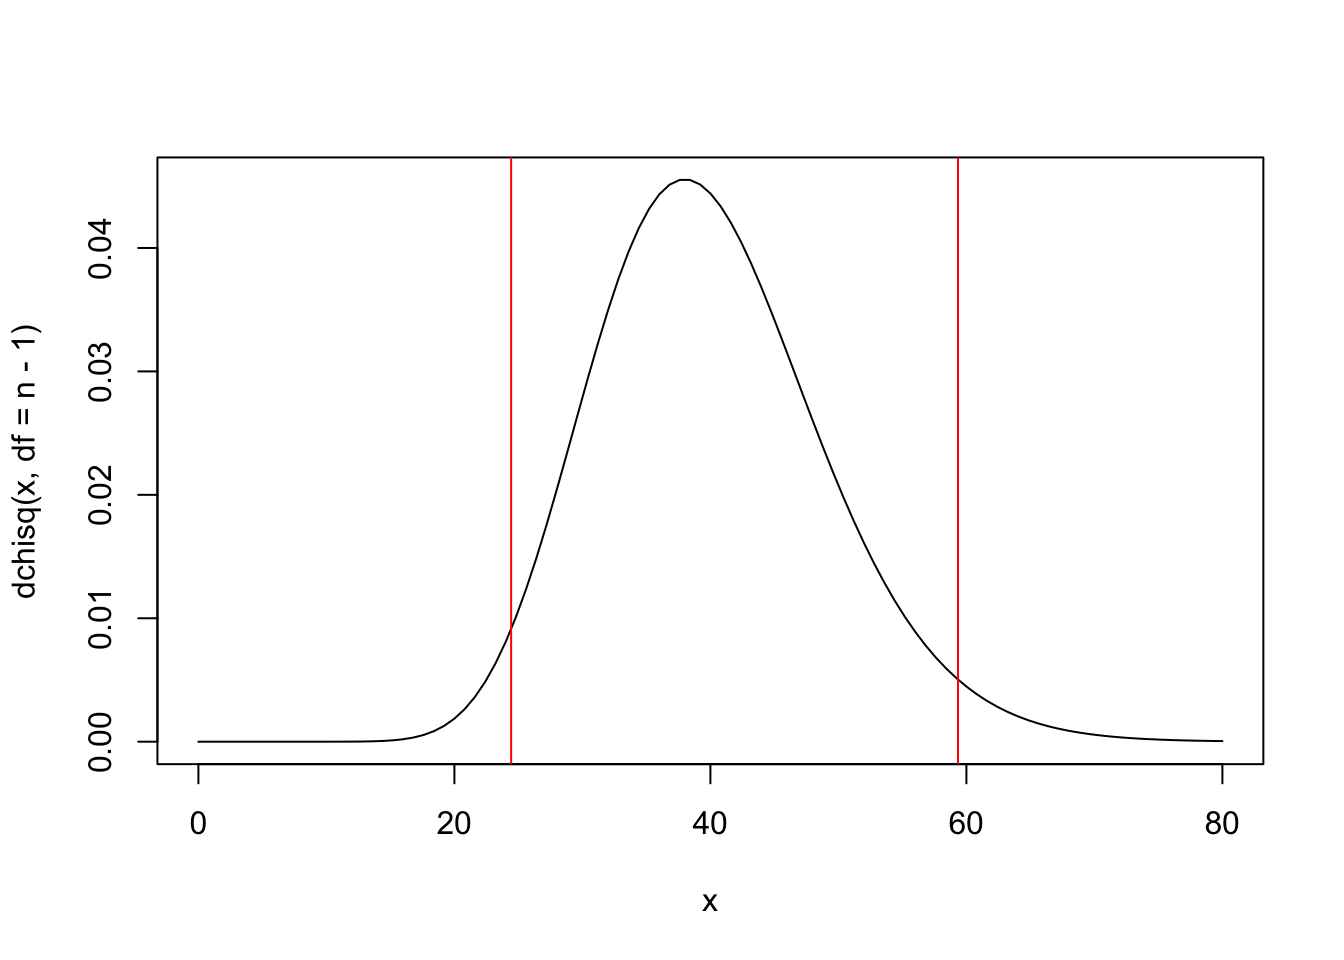
\includegraphics{_main_files/figure-latex/unnamed-chunk-101-1.pdf}

\begin{Shaded}
\begin{Highlighting}[]
\DecValTok{2}\OperatorTok{*}\KeywordTok{pchisq}\NormalTok{(quit, }\DataTypeTok{df =}\NormalTok{ n}\DecValTok{{-}1}\NormalTok{) }\CommentTok{\# p{-}value bilateral, H1: sigma\^{}2 ≠ 5, Eq. (3.24)}
\end{Highlighting}
\end{Shaded}

\begin{verbatim}
## [1] 0.0743
\end{verbatim}

\begin{Shaded}
\begin{Highlighting}[]
\KeywordTok{pchisq}\NormalTok{(quit, }\DataTypeTok{df =}\NormalTok{ n}\DecValTok{{-}1}\NormalTok{) }\CommentTok{\# p{-}value unilateral inferior, H1: sigma\^{}2 \textless{} 5, Eq. (3.25)}
\end{Highlighting}
\end{Shaded}

\begin{verbatim}
## [1] 0.0372
\end{verbatim}

\begin{Shaded}
\begin{Highlighting}[]
\DecValTok{1}\OperatorTok{{-}}\KeywordTok{pchisq}\NormalTok{(quit, }\DataTypeTok{df =}\NormalTok{ n}\DecValTok{{-}1}\NormalTok{) }\CommentTok{\# p{-}value unilateral superior, H1: sigma\^{}2 \textgreater{} 5, Eq. (3.26)}
\end{Highlighting}
\end{Shaded}

\begin{verbatim}
## [1] 0.963
\end{verbatim}

\begin{Shaded}
\begin{Highlighting}[]
\CommentTok{\# Via pacote DescTools}
\KeywordTok{library}\NormalTok{(DescTools)}
\KeywordTok{VarTest}\NormalTok{(x, }\DataTypeTok{sigma.squared =}\NormalTok{ sigma2\_}\DecValTok{0}\NormalTok{, }\DataTypeTok{alternative =} \StringTok{\textquotesingle{}two.sided\textquotesingle{}}\NormalTok{)}
\end{Highlighting}
\end{Shaded}

\begin{verbatim}
## 
##  One Sample Chi-Square test on variance
## 
## data:  x
## X-squared = 26, df = 40, p-value = 0.07
## alternative hypothesis: true variance is not equal to 5
## 95 percent confidence interval:
##  2.15 5.23
## sample estimates:
## variance of x 
##           3.2
\end{verbatim}

\begin{Shaded}
\begin{Highlighting}[]
\KeywordTok{VarTest}\NormalTok{(x, }\DataTypeTok{sigma.squared =}\NormalTok{ sigma2\_}\DecValTok{0}\NormalTok{, }\DataTypeTok{alternative =} \StringTok{\textquotesingle{}less\textquotesingle{}}\NormalTok{)}
\end{Highlighting}
\end{Shaded}

\begin{verbatim}
## 
##  One Sample Chi-Square test on variance
## 
## data:  x
## X-squared = 26, df = 40, p-value = 0.04
## alternative hypothesis: true variance is less than 5
## 95 percent confidence interval:
##  0.00 4.82
## sample estimates:
## variance of x 
##           3.2
\end{verbatim}

\begin{Shaded}
\begin{Highlighting}[]
\KeywordTok{VarTest}\NormalTok{(x, }\DataTypeTok{sigma.squared =}\NormalTok{ sigma2\_}\DecValTok{0}\NormalTok{, }\DataTypeTok{alternative =} \StringTok{\textquotesingle{}greater\textquotesingle{}}\NormalTok{)}
\end{Highlighting}
\end{Shaded}

\begin{verbatim}
## 
##  One Sample Chi-Square test on variance
## 
## data:  x
## X-squared = 26, df = 40, p-value = 1
## alternative hypothesis: true variance is greater than 5
## 95 percent confidence interval:
##  2.29  Inf
## sample estimates:
## variance of x 
##           3.2
\end{verbatim}

\begin{exercise}
\protect\hypertarget{exr:unnamed-chunk-102}{}{\label{exr:unnamed-chunk-102} }Suponha que o comprimento de peças em uma fábrica, simbolizado por \(X\), tenha distribuição normal de média e variância desconhecidas, anotado por \(X \sim \mathcal{N}(\mu,\sigma)\). A especificação indica média de 140cm, e desvio padrão de 7cm. Se em uma amostra de 64 peças foi observada uma média de \(\bar{x}=138\)cm e um desvio padrão de \(s=12\)cm, realize os testes de hipóteses apropriados para avaliar se as especificações estão sendo cumpridas. \(\\\)
\end{exercise}

\hypertarget{teste-5---teste-qui-quadrado-de-aderuxeancia-de-uma-amostra}{%
\subsubsection*{TESTE 5 - Teste qui-quadrado de aderência de uma amostra}\label{teste-5---teste-qui-quadrado-de-aderuxeancia-de-uma-amostra}}
\addcontentsline{toc}{subsubsection}{TESTE 5 - Teste qui-quadrado de aderência de uma amostra}

\textbf{Hipótese avaliada}\\
No universo representado por uma amostra, há diferença entre as frequências esperadas e observadas?

\textbf{Suposições}\\
S1. Os dados avaliados consistem em uma amostra aleatória de \(n\) observações (condicionalmente) independentes;\\
S2. Os dados representam frequências de \(k\) categorias mutuamente exclusivas.

\textbf{Estatística do teste}\\
Sob \(H_0: \pi_1=\pi_1^0, \pi_2=\pi_2^0, \ldots, \pi_k=\pi_k^0\),
\begin{equation}
\chi_{teste}^2 = \sum_{i=1}^{k} \frac{(O_{i}-E_{i})^2}{E_{i}} \sim \chi^2(gl),
\label{eq:qui-teste-ader-uni}
\end{equation}

onde \(E_{i}=n\pi_i^0\), \(k\) é o número de categorias e \(gl=k-1\) indica os \emph{graus de liberdade} que definem a distribuição \(\chi^2\).

\textbf{Valor-p}\\
Sob \(H_0: \pi_1=\pi_1^0, \pi_2=\pi_2^0, \ldots, \pi_k=\pi_k^0\),
\begin{equation}
\text{Valor-p} = Pr(\chi^2 \ge \chi_{teste}^2).
\label{eq:qui-teste-ader-uni-pvalue}
\end{equation}

\begin{example}
\protect\hypertarget{exm:qui-ader1}{}{\label{exm:qui-ader1} }(Adaptado de (Sheskin \protect\hyperlink{ref-sheskin2011handbook}{2011}, 278) - Teste qui-quadrado de aderência balanceado) Um dado é lançado 120 vezes, a fim de determinar se pode ou não ser considerado equilibrado. Os valores observados estão apresentados conforme tabela abaixo, e \(E_i=120 \times \frac{1}{6}=20, i \in \{1,2,3,4,5,6\}\).

\begin{longtable}[]{@{}ccccccc@{}}
\toprule
Face (\(i\)) & 1 & 2 & 3 & 4 & 5 & 6\tabularnewline
\midrule
\endhead
\(O_{i}\) & 20 & 14 & 18 & 17 & 22 & 29\tabularnewline
\(E_{i}\) & 20 & 20 & 20 & 20 & 20 & 20\tabularnewline
\bottomrule
\end{longtable}

Sob \(H_0: \pi_1=\frac{1}{6}, \pi_2=\frac{1}{6}, \pi_3=\frac{1}{6}, \pi_4=\frac{1}{6}, \pi_5=\frac{1}{6}, \pi_6=\frac{1}{6}\), \[\chi_{teste}^2 = \frac{(20-20)^2}{20} + \frac{(14-20)^2}{20} + \frac{(18-20)^2}{20} + \frac{(17-20)^2}{20} + \frac{(22-20)^2}{20} + \frac{(29-20)^2}{20} = 6.7.\] Considerando \(\alpha=0.05\) (unilateral superior, que é sempre o caso deste teste) e a tabela qui-quadrado com \(gl=6-1=5\), \(\chi_{cr\acute{\imath}tico}^2=11.07\). Como a estatística de teste não extrapola os valores críticos, i.e., \(6.7 < 11.07\), não se rejeita \(H_0\). Considerando a Equação \eqref{eq:qui-teste-ader-uni-pvalue} e a função \texttt{pchisq}, \[\text{Valor-p} = Pr(\chi^2 \ge 6.7) \approx 0.2439.\]
\emph{Decisão Estatística}: Não se rejeita \(H_0\) com \(\alpha=0.05\) pois \(6.7 < 11.07\) ou \(0.2439 > 0.05\).\\
\emph{Conclusão Experimental}: A amostra sugere que o dado deve ser equilibrado. \(\\\)
\end{example}

\begin{Shaded}
\begin{Highlighting}[]
\KeywordTok{curve}\NormalTok{(}\KeywordTok{dchisq}\NormalTok{(x, }\DataTypeTok{df=}\DecValTok{5}\NormalTok{), }\DecValTok{0}\NormalTok{, }\DecValTok{20}\NormalTok{) }\CommentTok{\# gráfico da qui\^{}2 com gl=6{-}1=5}
\NormalTok{(qui\_cr \textless{}{-}}\StringTok{ }\KeywordTok{qchisq}\NormalTok{(.}\DecValTok{95}\NormalTok{, }\DataTypeTok{df=}\DecValTok{5}\NormalTok{)) }\CommentTok{\# valor crítico}
\end{Highlighting}
\end{Shaded}

\begin{verbatim}
## [1] 11.1
\end{verbatim}

\begin{Shaded}
\begin{Highlighting}[]
\KeywordTok{abline}\NormalTok{(}\DataTypeTok{v =}\NormalTok{ qui\_cr, }\DataTypeTok{col=}\StringTok{\textquotesingle{}red\textquotesingle{}}\NormalTok{) }\CommentTok{\# valor crítico no gráfico}
\end{Highlighting}
\end{Shaded}

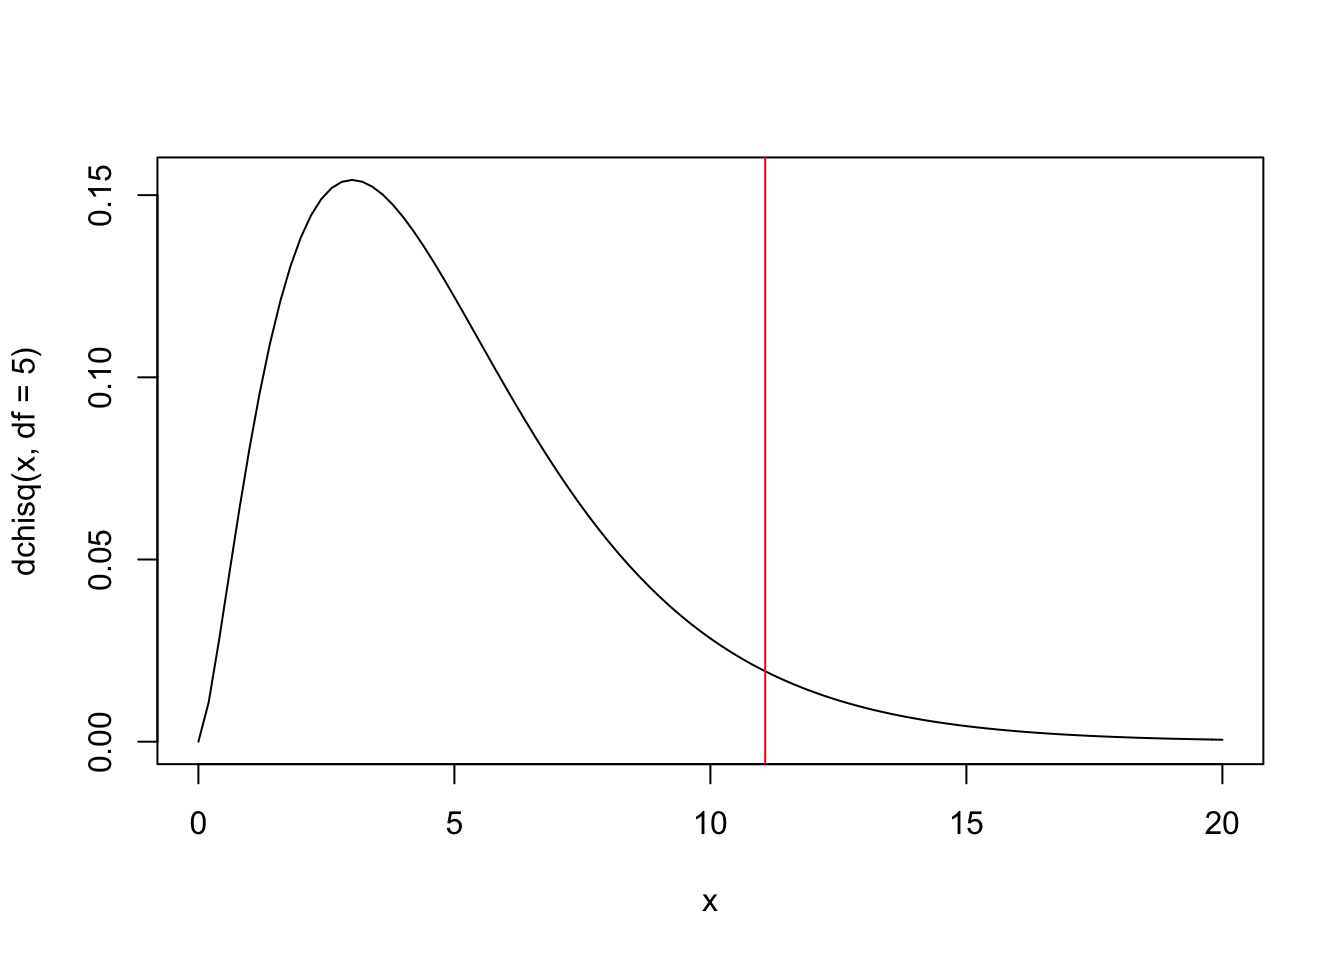
\includegraphics{_main_files/figure-latex/unnamed-chunk-104-1.pdf}

\begin{Shaded}
\begin{Highlighting}[]
\NormalTok{o \textless{}{-}}\StringTok{ }\KeywordTok{c}\NormalTok{(}\DecValTok{20}\NormalTok{,}\DecValTok{14}\NormalTok{,}\DecValTok{18}\NormalTok{,}\DecValTok{17}\NormalTok{,}\DecValTok{22}\NormalTok{,}\DecValTok{29}\NormalTok{)     }\CommentTok{\# Observados}
\NormalTok{n \textless{}{-}}\StringTok{ }\KeywordTok{sum}\NormalTok{(o)                   }\CommentTok{\# Tamanho da amostra}
\NormalTok{p \textless{}{-}}\StringTok{ }\KeywordTok{rep}\NormalTok{(}\DecValTok{1}\OperatorTok{/}\DecValTok{6}\NormalTok{,}\DecValTok{6}\NormalTok{)               }\CommentTok{\# Distribuição uniforme (dado equilibriado)}
\NormalTok{e \textless{}{-}}\StringTok{ }\NormalTok{n}\OperatorTok{*}\NormalTok{p                      }\CommentTok{\# Valores esperados se o dado for equilibrado}
\NormalTok{k \textless{}{-}}\StringTok{ }\KeywordTok{length}\NormalTok{(o)                }\CommentTok{\# Número de categorias}
\NormalTok{(qui \textless{}{-}}\StringTok{ }\KeywordTok{sum}\NormalTok{((o}\OperatorTok{{-}}\NormalTok{e)}\OperatorTok{\^{}}\DecValTok{2}\OperatorTok{/}\NormalTok{e))       }\CommentTok{\# Equação (3.25)}
\end{Highlighting}
\end{Shaded}

\begin{verbatim}
## [1] 6.7
\end{verbatim}

\begin{Shaded}
\begin{Highlighting}[]
\DecValTok{1}\OperatorTok{{-}}\KeywordTok{pchisq}\NormalTok{(qui,k}\DecValTok{{-}1}\NormalTok{)             }\CommentTok{\# p{-}value}
\end{Highlighting}
\end{Shaded}

\begin{verbatim}
## [1] 0.244
\end{verbatim}

\begin{Shaded}
\begin{Highlighting}[]
\KeywordTok{chisq.test}\NormalTok{(o)                 }\CommentTok{\# Pela função \textquotesingle{}chisq.test\textquotesingle{}}
\end{Highlighting}
\end{Shaded}

\begin{verbatim}
## 
##  Chi-squared test for given probabilities
## 
## data:  o
## X-squared = 7, df = 5, p-value = 0.2
\end{verbatim}

\begin{example}
\protect\hypertarget{exm:qui-ader2}{}{\label{exm:qui-ader2} }(Teste qui-quadrado de aderência desbalanceado) Gregor Mendel conduziu experimentos sobre hereditariedade em ervilhas. Em suma, as ervilhas podiam ser redondas (R) ou enrugadas (E), amarelas (A) ou verdes (V). Portanto, existem quatro combinações possíveis: RA, RV, EA, EV. Se sua teoria estivesse correta, as ervilhas seriam observadas na proporção de 9:3:3:1. Se o resultado do experimento produziu os seguintes dados observados, pode-se avaliar se há indícios da proporção considerada\footnote{Ainda que (Fisher \protect\hyperlink{ref-fisher1936has}{1936}) tenha posto dúvida sobre o trabalho de Mendel ao criar a noção do \emph{Paradoxo Mendeliano}, ou `bom demais para ser verdade'. Tal consideração tem bases eugenistas e incondicionalistas, calcada sob uma ótica ultrapassada assumida por Fisher e seus mentores, Karl Pearson e Francis Galton e já desmentida por acadêmicos como (Novitski \protect\hyperlink{ref-novitski2004fisher}{2004}) e (Hartl and Fairbanks \protect\hyperlink{ref-hartl2007mud}{2007}).}.

\begin{longtable}[]{@{}cccccc@{}}
\toprule
\(i\) & RA (1) & RV (2) & EA (3) & EV (4) & \textbf{\(n\)}\tabularnewline
\midrule
\endhead
\(O_i\) & 315 & 108 & 101 & 32 & \textbf{556}\tabularnewline
\(E_i\) & 312.75 & 104.25 & 104.25 & 34.75 & \textbf{556}\tabularnewline
\bottomrule
\end{longtable}

Sob \(H_0: \pi_1=\frac{9}{16}, \pi_2=\frac{3}{16}, \pi_3=\frac{3}{16}, \pi_4=\frac{1}{16}\), \[\chi_{teste}^2 = \frac{(315-312.75)^2}{312.75} + \frac{(108-104.25)^2}{104.25} + \frac{(101-104.25)^2}{104.25} + \frac{(32-34.75)^2}{34.75} \approx 0.47.\] Considerando \(\alpha=0.05\) (unilateral superior, que é sempre o caso deste teste) e a tabela qui-quadrado com \(gl=4-1=3\), \(\chi_{cr\acute{\imath}tico}^2=7.81\). Como a estatística de teste não extrapola os valores críticos, i.e., \(0.47 < 7.81\), não se rejeita \(H_0\). Considerando a Equação \eqref{eq:qui-teste-ader-uni-pvalue} e a função \texttt{pchisq}, \[\text{Valor-p} = Pr(\chi^2 \ge 0.47) \approx 0.9254.\]
\emph{Decisão Estatística}: Não se rejeita \(H_0\) com \(\alpha=0.05\) pois \(0.47 < 7.81\) ou \(0.9254 > 0.05\).\\
\emph{Conclusão Experimental}: A amostra sugere que a proporção das ervilhas deve ser 9:3:3:1. \(\\\)
\end{example}

\begin{Shaded}
\begin{Highlighting}[]
\NormalTok{o \textless{}{-}}\StringTok{ }\KeywordTok{c}\NormalTok{(}\DecValTok{315}\NormalTok{,}\DecValTok{108}\NormalTok{,}\DecValTok{101}\NormalTok{,}\DecValTok{32}\NormalTok{)      }\CommentTok{\# Observados}
\NormalTok{(n \textless{}{-}}\StringTok{ }\KeywordTok{sum}\NormalTok{(o))               }\CommentTok{\# Tamanho da amostra}
\end{Highlighting}
\end{Shaded}

\begin{verbatim}
## [1] 556
\end{verbatim}

\begin{Shaded}
\begin{Highlighting}[]
\NormalTok{(k \textless{}{-}}\StringTok{ }\KeywordTok{length}\NormalTok{(o))            }\CommentTok{\# Número de categorias}
\end{Highlighting}
\end{Shaded}

\begin{verbatim}
## [1] 4
\end{verbatim}

\begin{Shaded}
\begin{Highlighting}[]
\NormalTok{p \textless{}{-}}\StringTok{ }\KeywordTok{c}\NormalTok{(}\DecValTok{9}\OperatorTok{/}\DecValTok{16}\NormalTok{,}\DecValTok{3}\OperatorTok{/}\DecValTok{16}\NormalTok{,}\DecValTok{3}\OperatorTok{/}\DecValTok{16}\NormalTok{,}\DecValTok{1}\OperatorTok{/}\DecValTok{16}\NormalTok{) }\CommentTok{\# Proporção 9:3:3:1}
\NormalTok{(e \textless{}{-}}\StringTok{ }\NormalTok{n}\OperatorTok{*}\NormalTok{p)                  }\CommentTok{\# Valores esperados se a prop. for 9:3:3:1}
\end{Highlighting}
\end{Shaded}

\begin{verbatim}
## [1] 312.8 104.2 104.2  34.8
\end{verbatim}

\begin{Shaded}
\begin{Highlighting}[]
\NormalTok{(qui \textless{}{-}}\StringTok{ }\KeywordTok{sum}\NormalTok{((o}\OperatorTok{{-}}\NormalTok{e)}\OperatorTok{\^{}}\DecValTok{2}\OperatorTok{/}\NormalTok{e))     }\CommentTok{\# Estatística do teste}
\end{Highlighting}
\end{Shaded}

\begin{verbatim}
## [1] 0.47
\end{verbatim}

\begin{Shaded}
\begin{Highlighting}[]
\DecValTok{1}\OperatorTok{{-}}\KeywordTok{pchisq}\NormalTok{(qui,k}\DecValTok{{-}1}\NormalTok{)           }\CommentTok{\# Valor p}
\end{Highlighting}
\end{Shaded}

\begin{verbatim}
## [1] 0.925
\end{verbatim}

\begin{Shaded}
\begin{Highlighting}[]
\KeywordTok{chisq.test}\NormalTok{(o,}\DataTypeTok{p=}\NormalTok{p)           }\CommentTok{\# Pela função \textquotesingle{}chisq.test\textquotesingle{}}
\end{Highlighting}
\end{Shaded}

\begin{verbatim}
## 
##  Chi-squared test for given probabilities
## 
## data:  o
## X-squared = 0.5, df = 3, p-value = 0.9
\end{verbatim}

\hypertarget{testes-paramuxe9tricos-bivariados}{%
\subsection{Testes Paramétricos Bivariados}\label{testes-paramuxe9tricos-bivariados}}

\hypertarget{teste-6---teste-f-de-hartley-de-igualdade-de-variuxe2ncias}{%
\subsubsection*{TESTE 6 - Teste F (de Hartley) de igualdade de variâncias}\label{teste-6---teste-f-de-hartley-de-igualdade-de-variuxe2ncias}}
\addcontentsline{toc}{subsubsection}{TESTE 6 - Teste F (de Hartley) de igualdade de variâncias}

\textbf{Hipótese avaliada}\\
A variância do universo 1 é igual à variância do universo 2.

\textbf{Suposições}\\
S1. Os tamanhos de amostra \(n1\) e \(n2\) são similares.

\textbf{Estatística do teste}\\
Sob \(H_0: \sigma_1=\sigma_2\),
\begin{equation}
F_{max}=\frac{s_{max}^2}{s_{min}^2} \sim \mathcal{F}(n_{max}-1,n_{min}-1),
\label{eq:f-teste-var-bi}
\end{equation}

onde \(s_{max}^2\) e \(s_{min}^2\) são respectivamente a maior e menor variância amostral, e \(n_{max}\) e \(n_{min}\) correspondem respectivamente ao tamanho de amostra associado à amostra de maior e menor variância.

\textbf{Valor-p}\\
Sob \(H_0: \sigma_1=\sigma_2\),
\begin{equation}
\text{Valor-p} = 2Pr(F \ge F_{max}).
\label{eq:f-teste-var-bi-p-bi}
\end{equation}

Sob \(H_0: \sigma_1 \ge \sigma_2\),
\begin{equation}
\text{Valor-p} = Pr(F \ge F_{max}).
\label{eq:f-teste-var-bi-p-uni-inf}
\end{equation}

Sob \(H_0: \sigma_1 \le \sigma_2\),
\begin{equation}
\text{Valor-p} = Pr(F < F_{max}).
\label{eq:f-teste-var-bi-p-uni-sup}
\end{equation}

\begin{Shaded}
\begin{Highlighting}[]
\NormalTok{x \textless{}{-}}\StringTok{ }\DecValTok{1}\OperatorTok{:}\DecValTok{10}
\NormalTok{y \textless{}{-}}\StringTok{ }\KeywordTok{c}\NormalTok{(}\DecValTok{7}\OperatorTok{:}\DecValTok{20}\NormalTok{)}
\NormalTok{nx \textless{}{-}}\StringTok{ }\KeywordTok{length}\NormalTok{(x)}
\NormalTok{ny \textless{}{-}}\StringTok{ }\KeywordTok{length}\NormalTok{(y)}
\NormalTok{(Fmax \textless{}{-}}\StringTok{ }\KeywordTok{var}\NormalTok{(y)}\OperatorTok{/}\KeywordTok{var}\NormalTok{(x))}
\end{Highlighting}
\end{Shaded}

\begin{verbatim}
## [1] 1.91
\end{verbatim}

\begin{Shaded}
\begin{Highlighting}[]
\DecValTok{2}\OperatorTok{*}\NormalTok{(}\DecValTok{1}\OperatorTok{{-}}\KeywordTok{pf}\NormalTok{(Fmax,ny}\DecValTok{{-}1}\NormalTok{,nx}\DecValTok{{-}1}\NormalTok{)) }\CommentTok{\# H\_0: σ\_1 = σ\_2}
\end{Highlighting}
\end{Shaded}

\begin{verbatim}
## [1] 0.334
\end{verbatim}

\begin{Shaded}
\begin{Highlighting}[]
\DecValTok{1}\OperatorTok{{-}}\KeywordTok{pf}\NormalTok{(Fmax,ny}\DecValTok{{-}1}\NormalTok{,nx}\DecValTok{{-}1}\NormalTok{) }\CommentTok{\# H\_0: σ\_1 ≥ σ\_2}
\end{Highlighting}
\end{Shaded}

\begin{verbatim}
## [1] 0.167
\end{verbatim}

\begin{Shaded}
\begin{Highlighting}[]
\KeywordTok{pf}\NormalTok{(Fmax,ny}\DecValTok{{-}1}\NormalTok{,nx}\DecValTok{{-}1}\NormalTok{) }\CommentTok{\# H\_0: σ\_1 ≤ σ\_2}
\end{Highlighting}
\end{Shaded}

\begin{verbatim}
## [1] 0.833
\end{verbatim}

\begin{Shaded}
\begin{Highlighting}[]
\CommentTok{\# Utilizando a função var.test}
\KeywordTok{var.test}\NormalTok{(x,y) }\CommentTok{\# H\_0: σ\_1 = σ\_2}
\end{Highlighting}
\end{Shaded}

\begin{verbatim}
## 
##  F test to compare two variances
## 
## data:  x and y
## F = 0.5, num df = 9, denom df = 13, p-value = 0.3
## alternative hypothesis: true ratio of variances is not equal to 1
## 95 percent confidence interval:
##  0.158 2.007
## sample estimates:
## ratio of variances 
##              0.524
\end{verbatim}

\begin{Shaded}
\begin{Highlighting}[]
\KeywordTok{var.test}\NormalTok{(x,y, }\DataTypeTok{alternative =} \StringTok{\textquotesingle{}less\textquotesingle{}}\NormalTok{) }\CommentTok{\# H\_0: σ\_1 ≥ σ\_2}
\end{Highlighting}
\end{Shaded}

\begin{verbatim}
## 
##  F test to compare two variances
## 
## data:  x and y
## F = 0.5, num df = 9, denom df = 13, p-value = 0.2
## alternative hypothesis: true ratio of variances is less than 1
## 95 percent confidence interval:
##  0.0 1.6
## sample estimates:
## ratio of variances 
##              0.524
\end{verbatim}

\begin{Shaded}
\begin{Highlighting}[]
\KeywordTok{var.test}\NormalTok{(x,y, }\DataTypeTok{alternative =} \StringTok{\textquotesingle{}greater\textquotesingle{}}\NormalTok{) }\CommentTok{\# H\_0: σ\_1 ≤ σ\_2}
\end{Highlighting}
\end{Shaded}

\begin{verbatim}
## 
##  F test to compare two variances
## 
## data:  x and y
## F = 0.5, num df = 9, denom df = 13, p-value = 0.8
## alternative hypothesis: true ratio of variances is greater than 1
## 95 percent confidence interval:
##  0.193   Inf
## sample estimates:
## ratio of variances 
##              0.524
\end{verbatim}

\hypertarget{teste-7---teste-z-para-muxe9dias-de-duas-amostras-independentes}{%
\subsubsection*{\texorpdfstring{TESTE 7 - Teste \(z\) para médias de duas amostras independentes}{TESTE 7 - Teste z para médias de duas amostras independentes}}\label{teste-7---teste-z-para-muxe9dias-de-duas-amostras-independentes}}
\addcontentsline{toc}{subsubsection}{TESTE 7 - Teste \(z\) para médias de duas amostras independentes}

\textbf{Hipótese avaliada}\\
Duas amostras independentes representam duas populações com valores médios diferentes?

\textbf{Suposições}\\
S1. Cada amostra foi selecionada aleatoriamente da população que representa;\\
S2. A distribuição dos dados na população subjacente de cada amostra é normal;\\
S3. (\emph{Homogeneidade de variâncias}) A variância da população representada pela amostra 1 é igual à variância da população representada pela amostra 2 (\(\sigma_1^2=\sigma_2^2\)).

\textbf{Testes relacionados}\\
TESTE 16 - Teste dos postos de Mann-Whitney para duas amostras independentes

\textbf{Estatística do teste}\\
Sob \(H_0: \mu_1-\mu_2 = \Delta_0\),
\begin{equation}
z_{teste} = \frac{(\bar{x}_1-\bar{x}_2) - \Delta_0}{\sqrt{\frac{\sigma_1^2}{n_1}+\frac{\sigma_2^2}{n_2}}} \sim \mathcal{N}(0,1),
\label{eq:z-teste-media-bi}
\end{equation}

onde \(n_1\) e \(n_2\) são os tamanhos das amostras, \(\bar{x}_1\) e \(\bar{x}_2\) representam as médias amostrais e \(\sigma_1^2\) e \(\sigma_2^2\) são as variâncias universais dos universos 1 e 2.

\textbf{Valor-p}\\
Sob \(H_0: \mu_1-\mu_2 = \Delta_0\),
\begin{equation}
\text{Valor-p} = 2Pr(Z \le -|z_{teste}|).
\label{eq:z-teste-media-bi-p-bi}
\end{equation}

Sob \(H_0: \mu_1-\mu_2 \ge \Delta_0\),
\begin{equation}
\text{Valor-p} = Pr(Z \le z_{teste}).
\label{eq:z-teste-media-bi-p-uni-inf}
\end{equation}

Sob \(H_0: \mu_1-\mu_2 \le \Delta_0\),
\begin{equation}
\text{Valor-p} = Pr(Z \ge z_{teste}).
\label{eq:z-teste-media-bi-p-uni-sup}
\end{equation}

\begin{example}
\protect\hypertarget{exm:z-duas-medias-indep}{}{\label{exm:z-duas-medias-indep} }
\end{example}

\begin{Shaded}
\begin{Highlighting}[]
\NormalTok{x \textless{}{-}}\StringTok{ }\DecValTok{1}\OperatorTok{:}\DecValTok{10}
\NormalTok{y \textless{}{-}}\StringTok{ }\KeywordTok{c}\NormalTok{(}\DecValTok{7}\OperatorTok{:}\DecValTok{20}\NormalTok{)}
\NormalTok{nx \textless{}{-}}\StringTok{ }\KeywordTok{length}\NormalTok{(x)}
\NormalTok{ny \textless{}{-}}\StringTok{ }\KeywordTok{length}\NormalTok{(y)}
\NormalTok{mx \textless{}{-}}\StringTok{ }\KeywordTok{mean}\NormalTok{(x)}
\NormalTok{my \textless{}{-}}\StringTok{ }\KeywordTok{mean}\NormalTok{(y)}
\NormalTok{sigmax2 \textless{}{-}}\StringTok{ }\KeywordTok{var}\NormalTok{(x)}\OperatorTok{*}\NormalTok{(nx}\DecValTok{{-}1}\NormalTok{)}\OperatorTok{/}\NormalTok{nx}
\NormalTok{sigmay2 \textless{}{-}}\StringTok{ }\KeywordTok{var}\NormalTok{(y)}\OperatorTok{*}\NormalTok{(ny}\DecValTok{{-}1}\NormalTok{)}\OperatorTok{/}\NormalTok{ny}
\NormalTok{(zt \textless{}{-}}\StringTok{ }\NormalTok{(mx}\OperatorTok{{-}}\NormalTok{my)}\OperatorTok{/}\KeywordTok{sqrt}\NormalTok{(sigmax2}\OperatorTok{/}\NormalTok{nx}\OperatorTok{+}\NormalTok{sigmay2}\OperatorTok{/}\NormalTok{ny))}
\end{Highlighting}
\end{Shaded}

\begin{verbatim}
## [1] -5.68
\end{verbatim}

\begin{Shaded}
\begin{Highlighting}[]
\DecValTok{2}\OperatorTok{*}\KeywordTok{pnorm}\NormalTok{(}\OperatorTok{{-}}\KeywordTok{abs}\NormalTok{(zt)) }\CommentTok{\# H\_0: µ\_1{-}µ\_2 = 0}
\end{Highlighting}
\end{Shaded}

\begin{verbatim}
## [1] 1.37e-08
\end{verbatim}

\begin{Shaded}
\begin{Highlighting}[]
\KeywordTok{pnorm}\NormalTok{(zt)         }\CommentTok{\# H\_0: µ\_1{-}µ\_2 ≥ 0}
\end{Highlighting}
\end{Shaded}

\begin{verbatim}
## [1] 6.85e-09
\end{verbatim}

\begin{Shaded}
\begin{Highlighting}[]
\DecValTok{1}\OperatorTok{{-}}\KeywordTok{pnorm}\NormalTok{(zt)       }\CommentTok{\# H\_0: µ\_1{-}µ\_2 ≤ 0}
\end{Highlighting}
\end{Shaded}

\begin{verbatim}
## [1] 1
\end{verbatim}

\hypertarget{teste-8---teste-t-para-muxe9dias-de-duas-amostras-independentes}{%
\subsubsection*{\texorpdfstring{TESTE 8 - Teste \(t\) para médias de duas amostras independentes}{TESTE 8 - Teste t para médias de duas amostras independentes}}\label{teste-8---teste-t-para-muxe9dias-de-duas-amostras-independentes}}
\addcontentsline{toc}{subsubsection}{TESTE 8 - Teste \(t\) para médias de duas amostras independentes}

\textbf{Hipótese avaliada}\\
Duas amostras independentes representam duas populações com valores médios diferentes?

\textbf{Suposições}\\
S1. Cada amostra foi selecionada aleatoriamente da população que representa;\\
S2. A distribuição dos dados na população subjacente de cada amostra é normal.

\textbf{Testes relacionados}\\
TESTE 16 - Teste dos postos de Mann-Whitney para amostras independentes

\textbf{Estatística do teste}\\
Sob \(H_0: \mu_1-\mu_2 = \Delta_0\) e \(\sigma_1 = \sigma_2\),
\begin{equation}
t_{teste} = \frac{(\bar{x}_1-\bar{x}_2) - \Delta_0}{\sqrt{\left[ \frac{(n_1-1)s_1^2 + (n_2-1)s_2^2}{n_1+n_2-2} \right] \left[ \frac{1}{n_1}+\frac{1}{n_2} \right]}} \sim \mathcal{t}(gl).
\label{eq:t-teste-media-bi-vars-iguais}
\end{equation}

Sob \(H_0: \mu_1-\mu_2 = \Delta_0\) e \(\sigma_1 \ne \sigma_2\),
\begin{equation}
t_{teste} = \frac{(\bar{x}_1-\bar{x}_2) - \Delta_0}{\sqrt{\frac{s_1^2}{n_1} + \frac{s_2^2}{n_2}}} \sim \mathcal{t}(gl),
\label{eq:t-teste-media-bi-vars-dif}
\end{equation}

onde \(n_1\) e \(n_2\) são os tamanhos das amostras, \(\bar{x}_1\) e \(\bar{x}_2\) representam as médias amostrais e \(s_1^2\) e \(s_2^2\) são as variâncias amostrais dos universos 1 e 2. Se as variâncias forem admitidas iguais (\(\sigma_1 = \sigma_2\)), os graus de liberdade são calculados utilizando a expressão \[gl = n_1 + n_2-2.\] No caso de as variâncias serem admitidas diferentes (\(\sigma_1 \ne \sigma_2\)), calculam-se os graus de liberdade com a abordagem de Welch, dados por \[gl = \frac{\left( \frac{s_1^2}{n_1} + \frac{s_2^2}{n_2} \right)^2}{ \frac{(s_1^2/n_1)^2}{n_1-1} + \frac{(s_2^2/n_2)^2}{n_2-1}}.\]

\textbf{Valor-p}\\
Sob \(H_0: \mu_1-\mu_2 = \Delta_0\),
\begin{equation}
\text{Valor-p} = 2Pr(t \le -|t_{teste}|).
\label{eq:t-teste-media-bi-p-bi}
\end{equation}

Sob \(H_0: \mu_1-\mu_2 \ge \Delta_0\),
\begin{equation}
\text{Valor-p} = Pr(t \le t_{teste}).
\label{eq:t-teste-media-bi-p-uni-inf}
\end{equation}

Sob \(H_0: \mu_1-\mu_2 \le \Delta_0\),
\begin{equation}
\text{Valor-p} = Pr(t \ge t_{teste}).
\label{eq:t-teste-media-bi-p-uni-sup}
\end{equation}

\begin{example}
\protect\hypertarget{exm:t-duas-medias-indep}{}{\label{exm:t-duas-medias-indep} }
\end{example}

\begin{Shaded}
\begin{Highlighting}[]
\NormalTok{x \textless{}{-}}\StringTok{ }\DecValTok{1}\OperatorTok{:}\DecValTok{10}
\NormalTok{y \textless{}{-}}\StringTok{ }\KeywordTok{c}\NormalTok{(}\DecValTok{7}\OperatorTok{:}\DecValTok{20}\NormalTok{)}
\NormalTok{nx \textless{}{-}}\StringTok{ }\KeywordTok{length}\NormalTok{(x)}
\NormalTok{ny \textless{}{-}}\StringTok{ }\KeywordTok{length}\NormalTok{(y)}
\NormalTok{mx \textless{}{-}}\StringTok{ }\KeywordTok{mean}\NormalTok{(x)}
\NormalTok{my \textless{}{-}}\StringTok{ }\KeywordTok{mean}\NormalTok{(y)}
\NormalTok{sx2 \textless{}{-}}\StringTok{ }\KeywordTok{var}\NormalTok{(x)}
\NormalTok{sy2 \textless{}{-}}\StringTok{ }\KeywordTok{var}\NormalTok{(y)}
\NormalTok{sp2 \textless{}{-}}\StringTok{ }\NormalTok{((nx}\DecValTok{{-}1}\NormalTok{)}\OperatorTok{*}\NormalTok{sx2 }\OperatorTok{+}\StringTok{ }\NormalTok{(ny}\DecValTok{{-}1}\NormalTok{)}\OperatorTok{*}\NormalTok{sy2)}\OperatorTok{/}\NormalTok{(nx}\OperatorTok{+}\NormalTok{ny}\DecValTok{{-}2}\NormalTok{)}
\CommentTok{\# dando uma olhada nas variâncias}
\KeywordTok{var.test}\NormalTok{(x,y)}
\end{Highlighting}
\end{Shaded}

\begin{verbatim}
## 
##  F test to compare two variances
## 
## data:  x and y
## F = 0.5, num df = 9, denom df = 13, p-value = 0.3
## alternative hypothesis: true ratio of variances is not equal to 1
## 95 percent confidence interval:
##  0.158 2.007
## sample estimates:
## ratio of variances 
##              0.524
\end{verbatim}

\begin{Shaded}
\begin{Highlighting}[]
\CommentTok{\# estatística do teste para variâncias iguais}
\NormalTok{(tt\_igual \textless{}{-}}\StringTok{ }\NormalTok{(mx}\OperatorTok{{-}}\NormalTok{my)}\OperatorTok{/}\KeywordTok{sqrt}\NormalTok{(sp2}\OperatorTok{*}\NormalTok{(}\DecValTok{1}\OperatorTok{/}\NormalTok{nx}\OperatorTok{+}\DecValTok{1}\OperatorTok{/}\NormalTok{ny)))}
\end{Highlighting}
\end{Shaded}

\begin{verbatim}
## [1] -5.15
\end{verbatim}

\begin{Shaded}
\begin{Highlighting}[]
\CommentTok{\# estatística do teste para variâncias diferentes}
\NormalTok{(tt\_welch \textless{}{-}}\StringTok{ }\NormalTok{(mx}\OperatorTok{{-}}\NormalTok{my)}\OperatorTok{/}\KeywordTok{sqrt}\NormalTok{(sx2}\OperatorTok{/}\NormalTok{nx}\OperatorTok{+}\NormalTok{sy2}\OperatorTok{/}\NormalTok{ny)) }
\end{Highlighting}
\end{Shaded}

\begin{verbatim}
## [1] -5.43
\end{verbatim}

\begin{Shaded}
\begin{Highlighting}[]
\CommentTok{\# graus de liberdade para variâncias iguais}
\NormalTok{(gl\_igual \textless{}{-}}\StringTok{ }\NormalTok{nx}\OperatorTok{+}\NormalTok{ny}\DecValTok{{-}2}\NormalTok{) }
\end{Highlighting}
\end{Shaded}

\begin{verbatim}
## [1] 22
\end{verbatim}

\begin{Shaded}
\begin{Highlighting}[]
\CommentTok{\# graus de liberdade para variâncias diferentes}
\NormalTok{(gl\_welch \textless{}{-}}\StringTok{ }\NormalTok{(sx2}\OperatorTok{/}\NormalTok{nx}\OperatorTok{+}\NormalTok{sy2}\OperatorTok{/}\NormalTok{ny)}\OperatorTok{\^{}}\DecValTok{2}\OperatorTok{/}\NormalTok{((sx2}\OperatorTok{/}\NormalTok{nx)}\OperatorTok{\^{}}\DecValTok{2}\OperatorTok{/}\NormalTok{(nx}\DecValTok{{-}1}\NormalTok{) }\OperatorTok{+}\StringTok{ }\NormalTok{(sy2}\OperatorTok{/}\NormalTok{ny)}\OperatorTok{\^{}}\DecValTok{2}\OperatorTok{/}\NormalTok{(ny}\DecValTok{{-}1}\NormalTok{))) }
\end{Highlighting}
\end{Shaded}

\begin{verbatim}
## [1] 22
\end{verbatim}

\begin{Shaded}
\begin{Highlighting}[]
\CommentTok{\# H\_0: µ\_1{-}µ\_2 = 0, variâncias iguais}
\DecValTok{2}\OperatorTok{*}\KeywordTok{pt}\NormalTok{(}\OperatorTok{{-}}\KeywordTok{abs}\NormalTok{(tt\_igual), gl\_igual) }
\end{Highlighting}
\end{Shaded}

\begin{verbatim}
## [1] 3.69e-05
\end{verbatim}

\begin{Shaded}
\begin{Highlighting}[]
\CommentTok{\# H\_0: µ\_1{-}µ\_2 ≥ 0, variâncias iguais}
\KeywordTok{pt}\NormalTok{(tt\_igual, gl\_igual)         }
\end{Highlighting}
\end{Shaded}

\begin{verbatim}
## [1] 1.85e-05
\end{verbatim}

\begin{Shaded}
\begin{Highlighting}[]
\CommentTok{\# H\_0: µ\_1{-}µ\_2 ≤ 0, variâncias iguais}
\DecValTok{1}\OperatorTok{{-}}\KeywordTok{pt}\NormalTok{(tt\_igual, gl\_igual)       }
\end{Highlighting}
\end{Shaded}

\begin{verbatim}
## [1] 1
\end{verbatim}

\begin{Shaded}
\begin{Highlighting}[]
\CommentTok{\# H\_0: µ\_1{-}µ\_2 = 0, variâncias diferentes}
\DecValTok{2}\OperatorTok{*}\KeywordTok{pt}\NormalTok{(}\OperatorTok{{-}}\KeywordTok{abs}\NormalTok{(tt\_welch), gl\_welch) }
\end{Highlighting}
\end{Shaded}

\begin{verbatim}
## [1] 1.86e-05
\end{verbatim}

\begin{Shaded}
\begin{Highlighting}[]
\CommentTok{\# H\_0: µ\_1{-}µ\_2 ≥ 0, variâncias diferentes}
\KeywordTok{pt}\NormalTok{(tt\_welch, gl\_welch)         }
\end{Highlighting}
\end{Shaded}

\begin{verbatim}
## [1] 9.28e-06
\end{verbatim}

\begin{Shaded}
\begin{Highlighting}[]
\CommentTok{\# H\_0: µ\_1{-}µ\_2 ≤ 0, variâncias diferentes}
\DecValTok{1}\OperatorTok{{-}}\KeywordTok{pt}\NormalTok{(tt\_welch, gl\_welch)       }
\end{Highlighting}
\end{Shaded}

\begin{verbatim}
## [1] 1
\end{verbatim}

\begin{Shaded}
\begin{Highlighting}[]
\CommentTok{\# via t.test (facilita uma barbaridade!)}
\CommentTok{\# H\_0: µ\_1{-}µ\_2 = 0, σ\_1 = σ\_2}
\KeywordTok{t.test}\NormalTok{(}\DecValTok{1}\OperatorTok{:}\DecValTok{10}\NormalTok{, }\DataTypeTok{y =} \KeywordTok{c}\NormalTok{(}\DecValTok{7}\OperatorTok{:}\DecValTok{20}\NormalTok{), }\DataTypeTok{var.equal =}\NormalTok{ T)                          }
\end{Highlighting}
\end{Shaded}

\begin{verbatim}
## 
##  Two Sample t-test
## 
## data:  1:10 and c(7:20)
## t = -5, df = 22, p-value = 4e-05
## alternative hypothesis: true difference in means is not equal to 0
## 95 percent confidence interval:
##  -11.22  -4.78
## sample estimates:
## mean of x mean of y 
##       5.5      13.5
\end{verbatim}

\begin{Shaded}
\begin{Highlighting}[]
\CommentTok{\# H\_0: µ\_1{-}µ\_2 ≥ 0, σ\_1 = σ\_2}
\KeywordTok{t.test}\NormalTok{(}\DecValTok{1}\OperatorTok{:}\DecValTok{10}\NormalTok{, }\DataTypeTok{y =} \KeywordTok{c}\NormalTok{(}\DecValTok{7}\OperatorTok{:}\DecValTok{20}\NormalTok{), }\DataTypeTok{var.equal =}\NormalTok{ T, }\DataTypeTok{alternative =} \StringTok{\textquotesingle{}less\textquotesingle{}}\NormalTok{)    }
\end{Highlighting}
\end{Shaded}

\begin{verbatim}
## 
##  Two Sample t-test
## 
## data:  1:10 and c(7:20)
## t = -5, df = 22, p-value = 2e-05
## alternative hypothesis: true difference in means is less than 0
## 95 percent confidence interval:
##   -Inf -5.33
## sample estimates:
## mean of x mean of y 
##       5.5      13.5
\end{verbatim}

\begin{Shaded}
\begin{Highlighting}[]
\CommentTok{\# H\_0: µ\_1{-}µ\_2 ≤ 0, σ\_1 = σ\_2}
\KeywordTok{t.test}\NormalTok{(}\DecValTok{1}\OperatorTok{:}\DecValTok{10}\NormalTok{, }\DataTypeTok{y =} \KeywordTok{c}\NormalTok{(}\DecValTok{7}\OperatorTok{:}\DecValTok{20}\NormalTok{), }\DataTypeTok{var.equal =}\NormalTok{ T, }\DataTypeTok{alternative =} \StringTok{\textquotesingle{}greater\textquotesingle{}}\NormalTok{) }
\end{Highlighting}
\end{Shaded}

\begin{verbatim}
## 
##  Two Sample t-test
## 
## data:  1:10 and c(7:20)
## t = -5, df = 22, p-value = 1
## alternative hypothesis: true difference in means is greater than 0
## 95 percent confidence interval:
##  -10.7   Inf
## sample estimates:
## mean of x mean of y 
##       5.5      13.5
\end{verbatim}

\begin{Shaded}
\begin{Highlighting}[]
\CommentTok{\# H\_0: µ\_1{-}µ\_2 = 0, σ\_1 ≠ σ\_2}
\KeywordTok{t.test}\NormalTok{(}\DecValTok{1}\OperatorTok{:}\DecValTok{10}\NormalTok{, }\DataTypeTok{y =} \KeywordTok{c}\NormalTok{(}\DecValTok{7}\OperatorTok{:}\DecValTok{20}\NormalTok{), }\DataTypeTok{var.equal =}\NormalTok{ F)                          }
\end{Highlighting}
\end{Shaded}

\begin{verbatim}
## 
##  Welch Two Sample t-test
## 
## data:  1:10 and c(7:20)
## t = -5, df = 22, p-value = 2e-05
## alternative hypothesis: true difference in means is not equal to 0
## 95 percent confidence interval:
##  -11.05  -4.95
## sample estimates:
## mean of x mean of y 
##       5.5      13.5
\end{verbatim}

\begin{Shaded}
\begin{Highlighting}[]
\CommentTok{\# H\_0: µ\_1{-}µ\_2 ≥ 0, σ\_1 ≠ σ\_2  }
\KeywordTok{t.test}\NormalTok{(}\DecValTok{1}\OperatorTok{:}\DecValTok{10}\NormalTok{, }\DataTypeTok{y =} \KeywordTok{c}\NormalTok{(}\DecValTok{7}\OperatorTok{:}\DecValTok{20}\NormalTok{), }\DataTypeTok{var.equal =}\NormalTok{ F, }\DataTypeTok{alternative =} \StringTok{\textquotesingle{}less\textquotesingle{}}\NormalTok{)    }
\end{Highlighting}
\end{Shaded}

\begin{verbatim}
## 
##  Welch Two Sample t-test
## 
## data:  1:10 and c(7:20)
## t = -5, df = 22, p-value = 9e-06
## alternative hypothesis: true difference in means is less than 0
## 95 percent confidence interval:
##   -Inf -5.47
## sample estimates:
## mean of x mean of y 
##       5.5      13.5
\end{verbatim}

\begin{Shaded}
\begin{Highlighting}[]
\CommentTok{\# H\_0: µ\_1{-}µ\_2 ≤ 0, σ\_1 ≠ σ\_2}
\KeywordTok{t.test}\NormalTok{(}\DecValTok{1}\OperatorTok{:}\DecValTok{10}\NormalTok{, }\DataTypeTok{y =} \KeywordTok{c}\NormalTok{(}\DecValTok{7}\OperatorTok{:}\DecValTok{20}\NormalTok{), }\DataTypeTok{var.equal =}\NormalTok{ F, }\DataTypeTok{alternative =} \StringTok{\textquotesingle{}greater\textquotesingle{}}\NormalTok{) }
\end{Highlighting}
\end{Shaded}

\begin{verbatim}
## 
##  Welch Two Sample t-test
## 
## data:  1:10 and c(7:20)
## t = -5, df = 22, p-value = 1
## alternative hypothesis: true difference in means is greater than 0
## 95 percent confidence interval:
##  -10.5   Inf
## sample estimates:
## mean of x mean of y 
##       5.5      13.5
\end{verbatim}

\hypertarget{teste-9---teste-t-para-muxe9dias-de-duas-amostras-dependentespareadas}{%
\subsubsection*{\texorpdfstring{TESTE 9 - Teste \(t\) para médias de duas amostras dependentes/pareadas}{TESTE 9 - Teste t para médias de duas amostras dependentes/pareadas}}\label{teste-9---teste-t-para-muxe9dias-de-duas-amostras-dependentespareadas}}
\addcontentsline{toc}{subsubsection}{TESTE 9 - Teste \(t\) para médias de duas amostras dependentes/pareadas}

\textbf{Hipótese avaliada}\\
Duas amostras dependentes representam duas populações com médias diferentes?

\textbf{Suposições}\\
S1. Cada amostra foi selecionada aleatoriamente da população que representa;\\
S2. A distribuição dos dados na população subjacente de cada amostra é normal;\\
S3. (\emph{Homogeneidade de variâncias}) A variância da população representada pela amostra 1 é igual à variância da população representada pela amostra 2 (\(\sigma_1^2=\sigma_2^2\)).

\textbf{Testes relacionados}\\
TESTE 17 - Teste dos postos de Wilcoxon para amostras dependentes/pareadas.

\textbf{Estatística do teste}\\
Sob \(H_0: \mu_1-\mu_2 = \Delta_0\),
\begin{equation}
t_{teste} = \frac{\bar{D}-\Delta_0}{s_{\bar{D}}/\sqrt{n}} \sim \mathcal{t}(gl),
\label{eq:t-teste-medias-dep}
\end{equation}

onde \[\bar{D} = \frac{\sum D}{n},\] \(D=x_1-x_2\) e
\begin{equation}
s_{\bar{D}} = \sqrt{\left( \frac{\sum D^2}{n} - \bar{D}^2 \right) \left( \frac{n}{n-1} \right)}.
\label{eq:sD-medias-dep}
\end{equation}

\textbf{Valor-p}\\
Sob \(H_0: \mu_1-\mu_2 = \Delta_0\),
\begin{equation}
\text{Valor-p} = 2Pr(t \le -|t_{teste}|).
\label{eq:t-teste-medias-dep-p-bi}
\end{equation}

Sob \(H_0: \mu_1-\mu_2 \ge \Delta_0\),
\begin{equation}
\text{Valor-p} = Pr(t \le t_{teste}).
\label{eq:t-teste-medias-dep-p-uni-inf}
\end{equation}

Sob \(H_0: \mu_1-\mu_2 \le \Delta_0\),
\begin{equation}
\text{Valor-p} = Pr(t \ge t_{teste}).
\label{eq:t-teste-medias-dep-p-uni-sup}
\end{equation}

\begin{example}
\protect\hypertarget{exm:t-medias-dep}{}{\label{exm:t-medias-dep} }Adaptado de (Sheskin \protect\hyperlink{ref-sheskin2011handbook}{2011}, 764).
\end{example}

\begin{Shaded}
\begin{Highlighting}[]
\CommentTok{\# dados}
\NormalTok{x1 \textless{}{-}}\StringTok{ }\KeywordTok{c}\NormalTok{(}\DecValTok{9}\NormalTok{,}\DecValTok{2}\NormalTok{,}\DecValTok{1}\NormalTok{,}\DecValTok{4}\NormalTok{,}\DecValTok{6}\NormalTok{,}\DecValTok{4}\NormalTok{,}\DecValTok{7}\NormalTok{,}\DecValTok{8}\NormalTok{,}\DecValTok{5}\NormalTok{,}\DecValTok{1}\NormalTok{)}
\NormalTok{x2 \textless{}{-}}\StringTok{ }\KeywordTok{c}\NormalTok{(}\DecValTok{8}\NormalTok{,}\DecValTok{2}\NormalTok{,}\DecValTok{3}\NormalTok{,}\DecValTok{2}\NormalTok{,}\DecValTok{3}\NormalTok{,}\DecValTok{0}\NormalTok{,}\DecValTok{4}\NormalTok{,}\DecValTok{5}\NormalTok{,}\DecValTok{4}\NormalTok{,}\DecValTok{0}\NormalTok{)}
\CommentTok{\# validando suposições}
\KeywordTok{shapiro.test}\NormalTok{(x1)  }\CommentTok{\# S2, normalidade}
\end{Highlighting}
\end{Shaded}

\begin{verbatim}
## 
##  Shapiro-Wilk normality test
## 
## data:  x1
## W = 0.9, p-value = 0.6
\end{verbatim}

\begin{Shaded}
\begin{Highlighting}[]
\KeywordTok{shapiro.test}\NormalTok{(x2)  }\CommentTok{\# S2, normalidade}
\end{Highlighting}
\end{Shaded}

\begin{verbatim}
## 
##  Shapiro-Wilk normality test
## 
## data:  x2
## W = 0.9, p-value = 0.5
\end{verbatim}

\begin{Shaded}
\begin{Highlighting}[]
\NormalTok{g \textless{}{-}}\StringTok{ }\KeywordTok{as.factor}\NormalTok{(}\KeywordTok{rep}\NormalTok{(}\DecValTok{1}\OperatorTok{:}\DecValTok{2}\NormalTok{, }\DataTypeTok{each =} \KeywordTok{length}\NormalTok{(x1))) }\CommentTok{\# grupos 1 e 2}
\NormalTok{car}\OperatorTok{::}\KeywordTok{leveneTest}\NormalTok{(}\KeywordTok{c}\NormalTok{(x1,x2),g) }\CommentTok{\# S3, homogeneidade de variâncias}
\end{Highlighting}
\end{Shaded}

\begin{verbatim}
## Levene's Test for Homogeneity of Variance (center = median)
##       Df F value Pr(>F)
## group  1    0.78   0.39
##       18
\end{verbatim}

\begin{Shaded}
\begin{Highlighting}[]
\CommentTok{\# realizando o teste}
\NormalTok{D \textless{}{-}}\StringTok{ }\NormalTok{x1}\OperatorTok{{-}}\NormalTok{x2}
\NormalTok{n \textless{}{-}}\StringTok{ }\KeywordTok{length}\NormalTok{(D)}
\NormalTok{(mD \textless{}{-}}\StringTok{ }\KeywordTok{mean}\NormalTok{(D))}
\end{Highlighting}
\end{Shaded}

\begin{verbatim}
## [1] 1.6
\end{verbatim}

\begin{Shaded}
\begin{Highlighting}[]
\NormalTok{(sD \textless{}{-}}\StringTok{ }\KeywordTok{sd}\NormalTok{(D))}
\end{Highlighting}
\end{Shaded}

\begin{verbatim}
## [1] 1.78
\end{verbatim}

\begin{Shaded}
\begin{Highlighting}[]
\NormalTok{(tt \textless{}{-}}\StringTok{ }\NormalTok{mD}\OperatorTok{/}\NormalTok{(sD}\OperatorTok{/}\KeywordTok{sqrt}\NormalTok{(n)))}
\end{Highlighting}
\end{Shaded}

\begin{verbatim}
## [1] 2.85
\end{verbatim}

\begin{Shaded}
\begin{Highlighting}[]
\NormalTok{gl \textless{}{-}}\StringTok{ }\NormalTok{n}\DecValTok{{-}1}
\DecValTok{2}\OperatorTok{*}\NormalTok{(}\DecValTok{1}\OperatorTok{{-}}\KeywordTok{pt}\NormalTok{(tt, gl))}
\end{Highlighting}
\end{Shaded}

\begin{verbatim}
## [1] 0.0191
\end{verbatim}

\begin{Shaded}
\begin{Highlighting}[]
\CommentTok{\# via t.test (facilita uma barbaridade!)}
\KeywordTok{t.test}\NormalTok{(x1, x2, }\DataTypeTok{paired =}\NormalTok{ T)}
\end{Highlighting}
\end{Shaded}

\begin{verbatim}
## 
##  Paired t-test
## 
## data:  x1 and x2
## t = 3, df = 9, p-value = 0.02
## alternative hypothesis: true difference in means is not equal to 0
## 95 percent confidence interval:
##  0.329 2.871
## sample estimates:
## mean of the differences 
##                     1.6
\end{verbatim}

\begin{exercise}
\protect\hypertarget{exr:unnamed-chunk-110}{}{\label{exr:unnamed-chunk-110} }Faça o Exemplo \ref{exm:t-medias-dep} considerando \(H_0: \mu_1-\mu_2 \ge 0\) e \(H_0: \mu_1-\mu_2 \ge 0\).
\end{exercise}

\hypertarget{teste-10---testes-qui-quadrado-para-tabelas-l-times-c}{%
\subsubsection*{\texorpdfstring{TESTE 10 - Testes qui-quadrado para tabelas \(l \times c\)}{TESTE 10 - Testes qui-quadrado para tabelas l \textbackslash times c}}\label{teste-10---testes-qui-quadrado-para-tabelas-l-times-c}}
\addcontentsline{toc}{subsubsection}{TESTE 10 - Testes qui-quadrado para tabelas \(l \times c\)}

Estes testes são extensões do teste qui-quadrado de aderência de uma amostra (TESTE 5).

\textbf{Hipótese avaliada (geral)}\\
Na(s) população(ões) representada(s) pela(s) amostra(s) em uma tabela de contingência, as frequências de células observadas são diferentes das frequências esperadas?

\textbf{Hipóteses avaliadas (homogeneidade)}\\
As \(l\) amostras são ou não homogêneas com relação à proporção de observações em cada uma das \(c\) categorias? (ou)\\
Se os dados forem homogêneos, a proporção de observações na \(j\)-ésima categoria será igual em todas as \(l\) populações?

\textbf{Hipótese avaliada (independência)}\\
As duas dimensões/variáveis são independentes uma da outra?

\textbf{Suposições}\\
S1. Os dados avaliados representam uma amostra aleatória composta por \(n\) observações independentes;\\
S2. Os dados de frequência são categóricos para \(l \times c\) categorias mutuamente exclusivas;\\
S3. A frequência esperada de cada célula da tabela de contingência é de pelo menos 5;\\
S4. \textbf{(Homogeneidade)} As somas das linhas e colunas (somas marginais) \textbf{são} predeterminadas/fixas.\\
S4. \textbf{(Independência)} As somas das linhas e colunas (somas marginais) \textbf{não são} predeterminadas/fixas.

\textbf{Testes relacionados}
No caso de \(l>2\) ou \(c>2\) pode-se considerar uma análise \emph{post hoc}\footnote{A análise \emph{post hoc} é aplicada quando uma hipótese de múltiplas igualdades é rejeitada, admitindo-se que `há pelo menos dois grupos distintos'. Neste caso, fica a pergunta: quais grupos são distintos e em que grau? A terminologia é baseada na expressão latina que significa `depois disto'.} para o teste qui-quadrado de Pearson para dados de contagem, proposta por (Beasley and Schumacker \protect\hyperlink{ref-beasley1995multiple}{1995}), disponível no pacote \texttt{chisq.posthoc.test} (Ebbert \protect\hyperlink{ref-ebbert2019chisq}{2019}).

\textbf{Estatística do teste (sem correção de Yates)}\\
Sob \(H_0: O_{ij}=E_{ij}\) para todas as células ou \(H_0: \pi_{ij}=(\pi_{i\cdot})(\pi_{\cdot j})\) para todas as \(l \times c\) células,
\begin{equation}
\chi_{teste}^2 = \sum_{i=1}^{l} \sum_{j=1}^{c} \frac{(O_{ij}-E_{ij})^2}{E_{ij}} \sim \chi^2(gl),
\label{eq:qui-teste-qui-bi}
\end{equation}
onde
\begin{equation}
E_{ij}=\frac{(O_{i \cdot})(O_{\cdot j})}{n}.
\label{eq:valor-esperado}
\end{equation}
\(k\) é o número de categorias e \(gl=(l-1)(c-1)\) indica os \emph{graus de liberdade} que definem a distribuição \(\chi^2\).

\textbf{Estatística do teste (com correção de Yates)}\\
Sob \(H_0: O_{ij}=E_{ij}\) para todas as células ou \(H_0: \pi_{ij}=(\pi_{i\cdot})(\pi_{\cdot j})\) para todas as \(l \times c\) células,
\begin{equation}
\chi_{teste}^2 = \sum_{i=1}^{l} \sum_{j=1}^{c} \frac{(|O_{ij}-E_{ij}|-0.5)^2}{E_{ij}} \sim \chi^2(gl),
\label{eq:qui-teste-qui-bi-yates}
\end{equation}

\textbf{Estatística do teste simplificada para tabelas \(2 \times 2\) (sem correção de Yates)}\\
Sob \(H_0: O_{ij}=E_{ij}\) para todas as células ou \(H_0: \pi_{ij}=(\pi_{i\cdot})(\pi_{\cdot j})\) para todas as \(l \times c\) células,
\begin{equation}
\chi_{teste}^2 = \frac{n(ad-bc)^2}{(a+b)(c+d)(a+c)(b+d)},
\label{eq:qui-teste-qui-bi-simpl}
\end{equation}
onde \(a\), \(b\), \(c\) e \(d\) são as quantidades conforme tabela a seguir.

\begin{longtable}[]{@{}lccc@{}}
\toprule
& Coluna 1 & Coluna 2 & Total\tabularnewline
\midrule
\endhead
\textbf{Linha 1} & \(a\) & \(b\) & \textbf{a+b}\tabularnewline
\textbf{Linha 2} & \(c\) & \(d\) & \textbf{c+d}\tabularnewline
\textbf{Total} & \textbf{\(a+c\)} & \textbf{\(b+d\)} & \textbf{n}\tabularnewline
\bottomrule
\end{longtable}

\textbf{Estatística do teste simplificada para tabelas \(2 \times 2\) (com correção de Yates)}\\
Sob \(H_0: O_{ij}=E_{ij}\) para todas as células ou \(H_0: \pi_{ij}=(\pi_{i\cdot})(\pi_{\cdot j})\) para todas as \(l \times c\) células,
\begin{equation}
\chi_{teste}^2 = \frac{n(|ad-bc|-0.5n)^2}{(a+b)(c+d)(a+c)(b+d)}.
\label{eq:qui-teste-qui-bi-simpl-yates}
\end{equation}

\begin{example}
\protect\hypertarget{exm:altruismo}{}{\label{exm:altruismo} }(Adaptado de (Sheskin \protect\hyperlink{ref-sheskin2011handbook}{2011}, 639), teste de homogeneidade) Um pesquisador realiza um estudo para avaliar o efeito do ruído no comportamento altruísta. Cada um dos 200 sujeitos que participam do experimento é atribuído aleatoriamente a uma de duas condições experimentais. Os indivíduos em ambas as condições realizam um teste de uma hora, que é ostensivamente uma medida de inteligência. Durante o teste, os 100 indivíduos do Grupo 1 são expostos a um ruído alto e contínuo, que, segundo eles, é devido a um gerador com defeito. Os 100 sujeitos do Grupo 2 não são expostos a nenhum ruído durante o teste. Após a conclusão desta etapa do experimento, cada sujeito, ao deixar a sala, é confrontado por um homem de meia-idade cujo braço está em uma tipóia e que trabalha no experimentado. O homem pergunta ao sujeito se estaria disposto a ajudá-lo a carregar um pacote pesado para o carro. O número de sujeitos em cada grupo que ajudam o homem é registrado. Trinta dos 100 sujeitos que foram expostos ao ruído optaram por ajudar o homem, enquanto sessenta dos 100 sujeitos que não foram expostos ao ruído optaram por ajudar o homem. Os dados indicam que o comportamento altruísta é influenciado pelo ruído?

\begin{longtable}[]{@{}lccc@{}}
\toprule
& Ajudou & Não ajudou & Total\tabularnewline
\midrule
\endhead
Barulho & 30 & 70 & \textbf{100}\tabularnewline
Sem barulho & 60 & 40 & \textbf{100}\tabularnewline
\textbf{Total} & \textbf{90} & \textbf{110} & \textbf{200}\tabularnewline
\bottomrule
\end{longtable}
\end{example}

\begin{Shaded}
\begin{Highlighting}[]
\NormalTok{dados \textless{}{-}}\StringTok{ }\KeywordTok{matrix}\NormalTok{(}\KeywordTok{c}\NormalTok{(}\DecValTok{30}\NormalTok{,}\DecValTok{60}\NormalTok{,}\DecValTok{70}\NormalTok{,}\DecValTok{40}\NormalTok{), }\DataTypeTok{nrow=}\DecValTok{2}\NormalTok{)}
\KeywordTok{chisq.test}\NormalTok{(dados, }\DataTypeTok{correct =}\NormalTok{ F)}
\end{Highlighting}
\end{Shaded}

\begin{verbatim}
## 
##  Pearson's Chi-squared test
## 
## data:  dados
## X-squared = 18, df = 1, p-value = 2e-05
\end{verbatim}

\begin{Shaded}
\begin{Highlighting}[]
\KeywordTok{chisq.test}\NormalTok{(dados, }\DataTypeTok{correct =}\NormalTok{ T)}
\end{Highlighting}
\end{Shaded}

\begin{verbatim}
## 
##  Pearson's Chi-squared test with Yates' continuity correction
## 
## data:  dados
## X-squared = 17, df = 1, p-value = 4e-05
\end{verbatim}

\begin{example}
\protect\hypertarget{exm:intro-extro-politic}{}{\label{exm:intro-extro-politic} }(Adaptado de (Sheskin \protect\hyperlink{ref-sheskin2011handbook}{2011}, 640), teste de independência) Um pesquisador deseja testar se existe relação entre a dimensão da personalidade de introversão-extroversão e afiliação política. Duzentas pessoas são recrutadas para participar do estudo. Todos os sujeitos passam por um teste de personalidade com base no qual cada sujeito é classificado como introvertido ou extrovertido. Pede-se para cada sujeito indicar se ele ou ela é um democrata ou um republicano conforme tabela a seguir. Os dados indicam que existe uma relação significativa entre a afiliação política e se alguém é introvertido ou não extrovertido?

\begin{longtable}[]{@{}lccc@{}}
\toprule
& Democrata & Republicano & Total\tabularnewline
\midrule
\endhead
Introvertido & 30 & 70 & \textbf{100}\tabularnewline
Extrovertido & 60 & 40 & \textbf{100}\tabularnewline
\textbf{Total} & \textbf{90} & \textbf{110} & \textbf{200}\tabularnewline
\bottomrule
\end{longtable}
\end{example}

\begin{Shaded}
\begin{Highlighting}[]
\NormalTok{dados \textless{}{-}}\StringTok{ }\KeywordTok{matrix}\NormalTok{(}\KeywordTok{c}\NormalTok{(}\DecValTok{30}\NormalTok{,}\DecValTok{60}\NormalTok{,}\DecValTok{70}\NormalTok{,}\DecValTok{40}\NormalTok{), }\DataTypeTok{nrow=}\DecValTok{2}\NormalTok{)}
\KeywordTok{chisq.test}\NormalTok{(dados, }\DataTypeTok{correct =}\NormalTok{ F)}
\end{Highlighting}
\end{Shaded}

\begin{verbatim}
## 
##  Pearson's Chi-squared test
## 
## data:  dados
## X-squared = 18, df = 1, p-value = 2e-05
\end{verbatim}

\begin{Shaded}
\begin{Highlighting}[]
\KeywordTok{chisq.test}\NormalTok{(dados)}
\end{Highlighting}
\end{Shaded}

\begin{verbatim}
## 
##  Pearson's Chi-squared test with Yates' continuity correction
## 
## data:  dados
## X-squared = 17, df = 1, p-value = 4e-05
\end{verbatim}

\begin{exercise}
\protect\hypertarget{exr:exercicio-teste-qui-quadrado}{}{\label{exr:exercicio-teste-qui-quadrado} }Faça os cálculos dos Exemplos \ref{exm:altruismo} e \ref{exm:intro-extro-politic} utilizando todas as variações de estatísticas de teste.
\end{exercise}

\hypertarget{teste-11---teste-exato-de-fisher-para-tabelas-2-times-2}{%
\subsubsection*{\texorpdfstring{TESTE 11 - Teste exato de Fisher para tabelas \(2 \times 2\)}{TESTE 11 - Teste exato de Fisher para tabelas 2 \textbackslash times 2}}\label{teste-11---teste-exato-de-fisher-para-tabelas-2-times-2}}
\addcontentsline{toc}{subsubsection}{TESTE 11 - Teste exato de Fisher para tabelas \(2 \times 2\)}

Este teste pode ser pensado como a versão exata (não assintótica) para o teste qui-quadrado de homogeneidade do TESTE 10 .

\textbf{Hipótese avaliada (geral)}\\
Na(s) população(ões) representada(s) pela(s) amostra(s) em uma tabela de contingência, as frequências de células observadas são diferentes das frequências esperadas?

\textbf{Hipóteses avaliadas (homogeneidade)}\\
As \(l\) amostras são ou não homogêneas com relação à proporção de observações em cada uma das \(c\) categorias? (ou)\\
Se os dados forem homogêneos, a proporção de observações na \(j\)-ésima categoria será igual em todas as \(l\) populações?

\textbf{Suposições}\\
S1. Os dados avaliados representam uma amostra aleatória composta por \(n\) observações independentes;\\
S2. Os dados de frequência são categóricos para \(l \times c\) categorias mutuamente exclusivas;\\
S3. As somas das linhas e colunas (somas marginais) \textbf{são} predeterminadas/fixas.

\textbf{Valor-p para tabelas \(2 \times 2\)}\\
Sob \(H_0: O_{ij}=E_{ij}\) para todas as células ou \(H_0: \pi_{ij}=(\pi_{i\cdot})(\pi_{\cdot j})\) para todas as \(l \times c\) células,
\begin{equation}
P = \frac{(a+c)!(b+d)!(a+b)!(c+d)!}{n!a!b!c!d!},
\label{eq:qui-teste-exato-fisher}
\end{equation}
onde \(a\), \(b\), \(c\) e \(d\) são as quantidades conforme tabela a seguir.

\begin{longtable}[]{@{}lccc@{}}
\toprule
& Coluna 1 & Coluna 2 & Total\tabularnewline
\midrule
\endhead
\textbf{Linha 1} & \(a\) & \(b\) & \textbf{a+b}\tabularnewline
\textbf{Linha 2} & \(c\) & \(d\) & \textbf{c+d}\tabularnewline
\textbf{Total} & \textbf{\(a+c\)} & \textbf{\(b+d\)} & \textbf{n}\tabularnewline
\bottomrule
\end{longtable}

\begin{example}
\protect\hypertarget{exm:teste-exato-fisher}{}{\label{exm:teste-exato-fisher} }Pode-se resolver o Exemplo \ref{exm:altruismo} através do teste exato de Fisher.
\end{example}

\begin{Shaded}
\begin{Highlighting}[]
\NormalTok{dados \textless{}{-}}\StringTok{ }\KeywordTok{matrix}\NormalTok{(}\KeywordTok{c}\NormalTok{(}\DecValTok{30}\NormalTok{,}\DecValTok{60}\NormalTok{,}\DecValTok{70}\NormalTok{,}\DecValTok{40}\NormalTok{), }\DataTypeTok{nrow=}\DecValTok{2}\NormalTok{)}
\KeywordTok{fisher.test}\NormalTok{(dados)}
\end{Highlighting}
\end{Shaded}

\begin{verbatim}
## 
##  Fisher's Exact Test for Count Data
## 
## data:  dados
## p-value = 3e-05
## alternative hypothesis: true odds ratio is not equal to 1
## 95 percent confidence interval:
##  0.152 0.534
## sample estimates:
## odds ratio 
##      0.288
\end{verbatim}

\begin{exercise}
\protect\hypertarget{exr:exercicio-teste-exato-fisher}{}{\label{exr:exercicio-teste-exato-fisher} }Faça os cálculos do Exemplo \ref{exm:teste-exato-fisher}.
\end{exercise}

\hypertarget{testes-paramuxe9tricos-multivariados}{%
\subsection{Testes Paramétricos Multivariados}\label{testes-paramuxe9tricos-multivariados}}

\hypertarget{teste-12---anuxe1lise-de-variuxe2ncia-anova-de-um-fator-entre-sujeitos}{%
\subsubsection*{TESTE 12 - Análise de Variância (ANOVA) de um fator entre sujeitos}\label{teste-12---anuxe1lise-de-variuxe2ncia-anova-de-um-fator-entre-sujeitos}}
\addcontentsline{toc}{subsubsection}{TESTE 12 - Análise de Variância (ANOVA) de um fator entre sujeitos}

\textbf{Hipótese avaliada}\\
Em um conjunto de \(k \ge 2\) grupos independentes, há pelo menos dois com médias distintas?

\textbf{Suposições}\\
S1. Cada amostra foi selecionada aleatoriamente da população que representa;\\
S2. A distribuição dos dados na população subjacente da qual cada uma das amostras é derivada é normal;\\
S3. (\emph{Homogeneidade de variâncias}) A variância da população representada pelas \(k\) amostras são iguais entre si. (\(\sigma_1^2=\sigma_2^2=\cdots=\sigma_k^2\)).

\textbf{Testes relacionados}\\
TESTE 19 - Teste de Kruskal-Wallis de um fator entre sujeitos

\textbf{Estatística do teste}\\
Sob \(H_0: \mu_1=\mu_2=\cdots=\mu_k\),
\begin{equation}
F_{teste} = \frac{MQ_{EG}}{MQ_{IG}} \sim \mathcal{F}(gl_{EG},gl_{IG}),
\label{eq:anova-1fat-entre-suj}
\end{equation}

onde \(MQ_{EG}\) é a média quadrática entre grupos dada por
\begin{equation}
MQ_{EG} = \frac{SQ_{EG}}{gl_{EG}},
\label{eq:mq-entre}
\end{equation}

onde \(SQ_{EG}\) é a soma de quadrados entre grupos dada por
\begin{equation}
SQ_{EG} = \sum_{j=1}^k \left[ \frac{(\sum x_j)^2}{n_j} \right] - \frac{(\sum x_T)^2}{n},
\label{eq:sq-entre}
\end{equation}

\(MQ_{IG}\) é a média quadrática intra grupos dada por
\begin{equation}
MQ_{IG} = \frac{SQ_{IG}}{gl_{IG}},
\label{eq:mq-intra}
\end{equation}

onde \(SQ_{IG}\) é a soma de quadrados intra grupos dada por
\begin{equation}
SQ_{IG} = \sum_{j=1}^k \left[ \sum x_{j}^2 - \frac{(\sum x_j)^2}{n_j} \right],
\label{eq:sq-intra}
\end{equation}

\(gl_{EG}=k-1\) são os graus de liberdade entre grupos, \(gl_{IG}=n-k\) são os graus de liberdade intra grupos. Sabe-se também que
onde \(SQ_{IG}\) é a soma de quadrados intra grupos dada por
\begin{equation}
SQ_{T} = SQ_{EG} + SQ_{IG} = \sum x_{T}^2 - \frac{(\sum x_T)^2}{n}.
\label{eq:sq-t}
\end{equation}

\begin{example}
\protect\hypertarget{exm:anova-entre-suj}{}{\label{exm:anova-entre-suj} }(Adaptado de (Sheskin \protect\hyperlink{ref-sheskin2011handbook}{2011}, 886)) Um psicólogo realiza um estudo para determinar se o ruído pode ou não inibir o aprendizado. Cada um de 15 sujeitos é atribuído aleatoriamente a um dos três grupos. Cada sujeito tem 20 minutos para memorizar uma lista de 10 sílabas sem sentido, que ela diz que será testada no dia seguinte. Os cinco sujeitos atribuídos ao Grupo 1, a condição sem ruído, estudam a lista de sílabas sem sentido enquanto estão em uma sala silenciosa. Os cinco sujeitos designados para o Grupo 2, a condição de ruído moderado, estudam a lista de sílabas sem sentido enquanto ouvem música clássica. Os cinco sujeitos designados para o Grupo 3, a condição de ruído extremo, estudam a lista de sílabas sem sentido enquanto ouvem música rock. O número de sílabas sem sentido lembradas corretamente pelos 15 sujeitos segue: Grupo 1: 8,10,9,10,9; Grupo 2: 7,8,5,8,5; Grupo 3: 4,8,7,5,7. Os dados indicam que o ruído influenciou o desempenho dos sujeitos?
\end{example}

\begin{Shaded}
\begin{Highlighting}[]
\CommentTok{\# dados}
\NormalTok{x \textless{}{-}}\StringTok{ }\KeywordTok{c}\NormalTok{(}\DecValTok{8}\NormalTok{,}\DecValTok{10}\NormalTok{,}\DecValTok{9}\NormalTok{,}\DecValTok{10}\NormalTok{,}\DecValTok{9}\NormalTok{, }\DecValTok{7}\NormalTok{,}\DecValTok{8}\NormalTok{,}\DecValTok{5}\NormalTok{,}\DecValTok{8}\NormalTok{,}\DecValTok{5}\NormalTok{, }\DecValTok{4}\NormalTok{,}\DecValTok{8}\NormalTok{,}\DecValTok{7}\NormalTok{,}\DecValTok{5}\NormalTok{,}\DecValTok{7}\NormalTok{)}
\NormalTok{g \textless{}{-}}\StringTok{ }\KeywordTok{as.factor}\NormalTok{(}\KeywordTok{rep}\NormalTok{(}\DecValTok{1}\OperatorTok{:}\DecValTok{3}\NormalTok{, }\DataTypeTok{each =} \DecValTok{5}\NormalTok{))}
\NormalTok{(k \textless{}{-}}\StringTok{ }\KeywordTok{length}\NormalTok{(}\KeywordTok{unique}\NormalTok{(g))) }\CommentTok{\# número de grupos}
\end{Highlighting}
\end{Shaded}

\begin{verbatim}
## [1] 3
\end{verbatim}

\begin{Shaded}
\begin{Highlighting}[]
\KeywordTok{boxplot}\NormalTok{(x }\OperatorTok{\textasciitilde{}}\StringTok{ }\NormalTok{g)}
\end{Highlighting}
\end{Shaded}

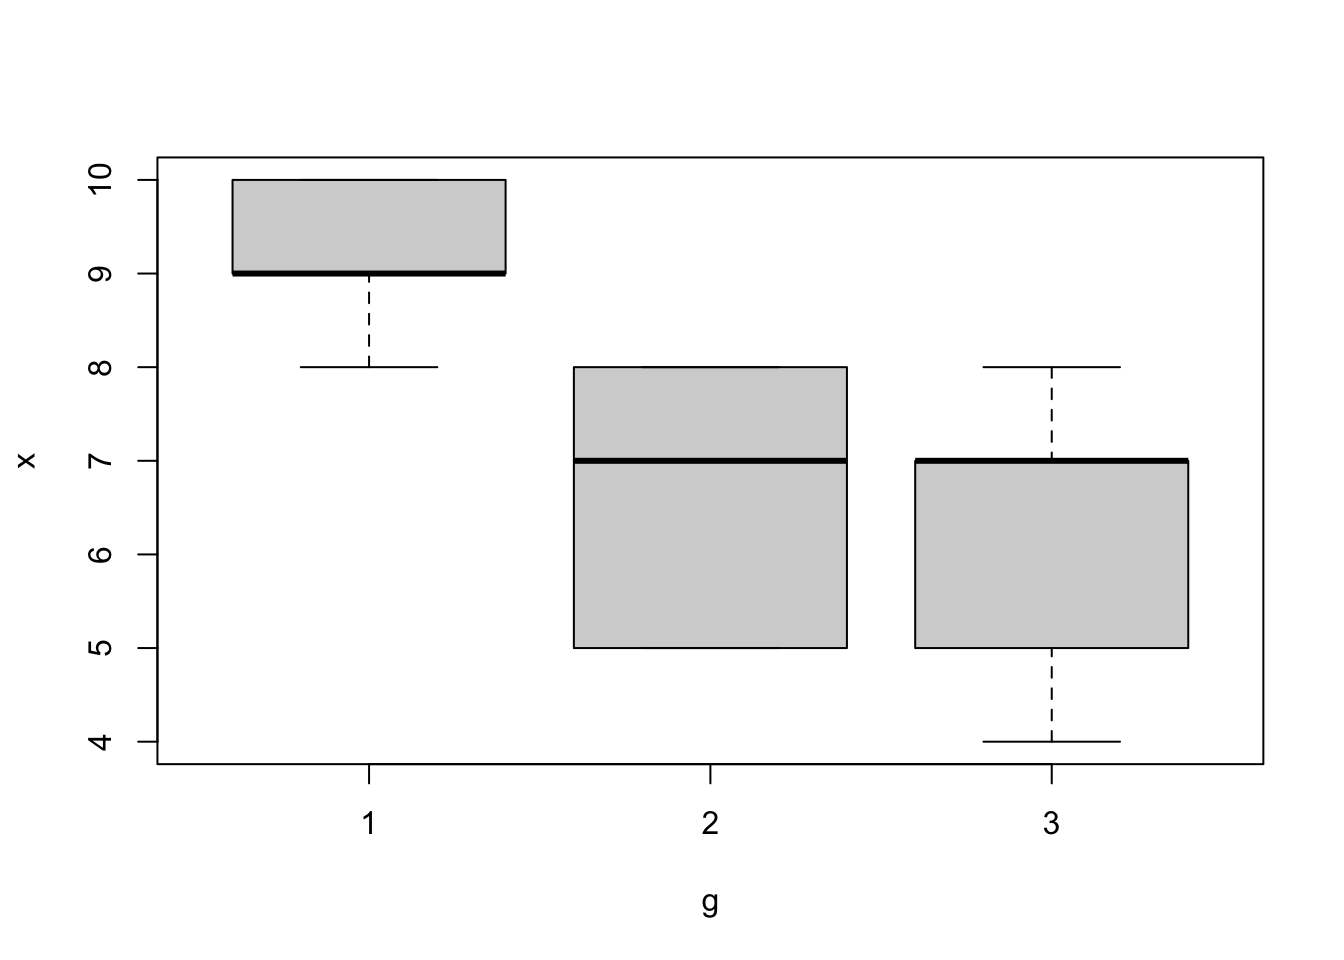
\includegraphics{_main_files/figure-latex/unnamed-chunk-114-1.pdf}

\begin{Shaded}
\begin{Highlighting}[]
\CommentTok{\# validando suposições, veja ?by}
\KeywordTok{by}\NormalTok{(x,g,shapiro.test)  }\CommentTok{\# S2, normalidade}
\end{Highlighting}
\end{Shaded}

\begin{verbatim}
## g: 1
## 
##  Shapiro-Wilk normality test
## 
## data:  dd[x, ]
## W = 0.9, p-value = 0.3
## 
## --------------------------------------------------------------------------------------------- 
## g: 2
## 
##  Shapiro-Wilk normality test
## 
## data:  dd[x, ]
## W = 0.8, p-value = 0.09
## 
## --------------------------------------------------------------------------------------------- 
## g: 3
## 
##  Shapiro-Wilk normality test
## 
## data:  dd[x, ]
## W = 0.9, p-value = 0.5
\end{verbatim}

\begin{Shaded}
\begin{Highlighting}[]
\NormalTok{car}\OperatorTok{::}\KeywordTok{leveneTest}\NormalTok{(x,g)  }\CommentTok{\# S3, homogeneidade de variâncias}
\end{Highlighting}
\end{Shaded}

\begin{verbatim}
## Levene's Test for Homogeneity of Variance (center = median)
##       Df F value Pr(>F)
## group  2    0.67   0.53
##       12
\end{verbatim}

\begin{Shaded}
\begin{Highlighting}[]
\CommentTok{\# cálculos}
\NormalTok{(soma \textless{}{-}}\StringTok{ }\KeywordTok{by}\NormalTok{(x,g,sum))     }\CommentTok{\# soma por grupo}
\end{Highlighting}
\end{Shaded}

\begin{verbatim}
## g: 1
## [1] 46
## --------------------------------------------------------------------------------------------- 
## g: 2
## [1] 33
## --------------------------------------------------------------------------------------------- 
## g: 3
## [1] 31
\end{verbatim}

\begin{Shaded}
\begin{Highlighting}[]
\NormalTok{(media \textless{}{-}}\StringTok{ }\KeywordTok{by}\NormalTok{(x,g,mean))   }\CommentTok{\# média por grupo}
\end{Highlighting}
\end{Shaded}

\begin{verbatim}
## g: 1
## [1] 9.2
## --------------------------------------------------------------------------------------------- 
## g: 2
## [1] 6.6
## --------------------------------------------------------------------------------------------- 
## g: 3
## [1] 6.2
\end{verbatim}

\begin{Shaded}
\begin{Highlighting}[]
\NormalTok{(soma2 \textless{}{-}}\StringTok{ }\KeywordTok{by}\NormalTok{(x}\OperatorTok{\^{}}\DecValTok{2}\NormalTok{,g,sum))  }\CommentTok{\# soma ao quadrado por grupo}
\end{Highlighting}
\end{Shaded}

\begin{verbatim}
## g: 1
## [1] 426
## --------------------------------------------------------------------------------------------- 
## g: 2
## [1] 227
## --------------------------------------------------------------------------------------------- 
## g: 3
## [1] 203
\end{verbatim}

\begin{Shaded}
\begin{Highlighting}[]
\NormalTok{(n \textless{}{-}}\StringTok{ }\KeywordTok{by}\NormalTok{(x,g,length))     }\CommentTok{\# tamanho da amostra por grupo}
\end{Highlighting}
\end{Shaded}

\begin{verbatim}
## g: 1
## [1] 5
## --------------------------------------------------------------------------------------------- 
## g: 2
## [1] 5
## --------------------------------------------------------------------------------------------- 
## g: 3
## [1] 5
\end{verbatim}

\begin{Shaded}
\begin{Highlighting}[]
\NormalTok{(somaT \textless{}{-}}\StringTok{ }\KeywordTok{sum}\NormalTok{(soma))      }\CommentTok{\# soma total}
\end{Highlighting}
\end{Shaded}

\begin{verbatim}
## [1] 110
\end{verbatim}

\begin{Shaded}
\begin{Highlighting}[]
\NormalTok{(soma2T \textless{}{-}}\StringTok{ }\KeywordTok{sum}\NormalTok{(soma2))    }\CommentTok{\# soma ao quadrado total}
\end{Highlighting}
\end{Shaded}

\begin{verbatim}
## [1] 856
\end{verbatim}

\begin{Shaded}
\begin{Highlighting}[]
\NormalTok{(nT \textless{}{-}}\StringTok{ }\KeywordTok{sum}\NormalTok{(n))            }\CommentTok{\# tamanho total da amostra}
\end{Highlighting}
\end{Shaded}

\begin{verbatim}
## [1] 15
\end{verbatim}

\begin{Shaded}
\begin{Highlighting}[]
\NormalTok{(sqt \textless{}{-}}\StringTok{ }\NormalTok{soma2T }\OperatorTok{{-}}\StringTok{ }\NormalTok{somaT}\OperatorTok{\^{}}\DecValTok{2}\OperatorTok{/}\NormalTok{nT) }\CommentTok{\# SQ\_T pela Eq. (3.50)}
\end{Highlighting}
\end{Shaded}

\begin{verbatim}
## [1] 49.3
\end{verbatim}

\begin{Shaded}
\begin{Highlighting}[]
\NormalTok{(sqeg \textless{}{-}}\StringTok{ }\KeywordTok{sum}\NormalTok{(soma}\OperatorTok{\^{}}\DecValTok{2}\OperatorTok{/}\NormalTok{n) }\OperatorTok{{-}}\StringTok{ }\NormalTok{somaT}\OperatorTok{\^{}}\DecValTok{2}\OperatorTok{/}\NormalTok{nT) }\CommentTok{\# SQ\_\{EG\} pela Eq. (3.47)}
\end{Highlighting}
\end{Shaded}

\begin{verbatim}
## [1] 26.5
\end{verbatim}

\begin{Shaded}
\begin{Highlighting}[]
\NormalTok{(sqig \textless{}{-}}\StringTok{ }\KeywordTok{sum}\NormalTok{(soma2 }\OperatorTok{{-}}\StringTok{ }\NormalTok{soma}\OperatorTok{\^{}}\DecValTok{2}\OperatorTok{/}\NormalTok{n)) }\CommentTok{\# SQ\_\{IG\} pela Eq. (3.49)}
\end{Highlighting}
\end{Shaded}

\begin{verbatim}
## [1] 22.8
\end{verbatim}

\begin{Shaded}
\begin{Highlighting}[]
\NormalTok{sqt }\OperatorTok{{-}}\StringTok{ }\NormalTok{sqeg }\CommentTok{\# SQ\_\{IG\} pela Eq. (3.50)}
\end{Highlighting}
\end{Shaded}

\begin{verbatim}
## [1] 22.8
\end{verbatim}

\begin{Shaded}
\begin{Highlighting}[]
\NormalTok{(gleg \textless{}{-}}\StringTok{ }\NormalTok{k}\DecValTok{{-}1}\NormalTok{) }\CommentTok{\# gl\_\{EG\}}
\end{Highlighting}
\end{Shaded}

\begin{verbatim}
## [1] 2
\end{verbatim}

\begin{Shaded}
\begin{Highlighting}[]
\NormalTok{(glig \textless{}{-}}\StringTok{ }\NormalTok{nT}\OperatorTok{{-}}\NormalTok{k) }\CommentTok{\# gl\_\{IG\}}
\end{Highlighting}
\end{Shaded}

\begin{verbatim}
## [1] 12
\end{verbatim}

\begin{Shaded}
\begin{Highlighting}[]
\NormalTok{(mqeg \textless{}{-}}\StringTok{ }\NormalTok{sqeg}\OperatorTok{/}\NormalTok{gleg) }\CommentTok{\# MQ\_\{EG\} pela Eq. (3.46)}
\end{Highlighting}
\end{Shaded}

\begin{verbatim}
## [1] 13.3
\end{verbatim}

\begin{Shaded}
\begin{Highlighting}[]
\NormalTok{(mqig \textless{}{-}}\StringTok{ }\NormalTok{sqig}\OperatorTok{/}\NormalTok{glig) }\CommentTok{\# MQ\_\{IG\} pela Eq. (3.48)}
\end{Highlighting}
\end{Shaded}

\begin{verbatim}
## [1] 1.9
\end{verbatim}

\begin{Shaded}
\begin{Highlighting}[]
\NormalTok{(Ft \textless{}{-}}\StringTok{ }\NormalTok{mqeg}\OperatorTok{/}\NormalTok{mqig) }\CommentTok{\# estatística do teste pela Eq. (3.45)}
\end{Highlighting}
\end{Shaded}

\begin{verbatim}
## [1] 6.98
\end{verbatim}

\begin{Shaded}
\begin{Highlighting}[]
\DecValTok{2}\OperatorTok{*}\KeywordTok{df}\NormalTok{(Ft,gleg,glig)}
\end{Highlighting}
\end{Shaded}

\begin{verbatim}
## [1] 0.00901
\end{verbatim}

\begin{Shaded}
\begin{Highlighting}[]
\CommentTok{\# pela função aov}
\KeywordTok{summary}\NormalTok{(anova1 \textless{}{-}}\StringTok{ }\KeywordTok{aov}\NormalTok{(x }\OperatorTok{\textasciitilde{}}\StringTok{ }\NormalTok{g))}
\end{Highlighting}
\end{Shaded}

\begin{verbatim}
##             Df Sum Sq Mean Sq F value Pr(>F)   
## g            2   26.5    13.3    6.98 0.0097 **
## Residuals   12   22.8     1.9                  
## ---
## Signif. codes:  0 '***' 0.001 '**' 0.01 '*' 0.05 '.' 0.1 ' ' 1
\end{verbatim}

\begin{Shaded}
\begin{Highlighting}[]
\KeywordTok{par}\NormalTok{(}\DataTypeTok{mfrow=}\KeywordTok{c}\NormalTok{(}\DecValTok{2}\NormalTok{,}\DecValTok{2}\NormalTok{))}
\KeywordTok{plot}\NormalTok{(anova1, }\DataTypeTok{which=}\DecValTok{1}\OperatorTok{:}\DecValTok{4}\NormalTok{)}
\end{Highlighting}
\end{Shaded}

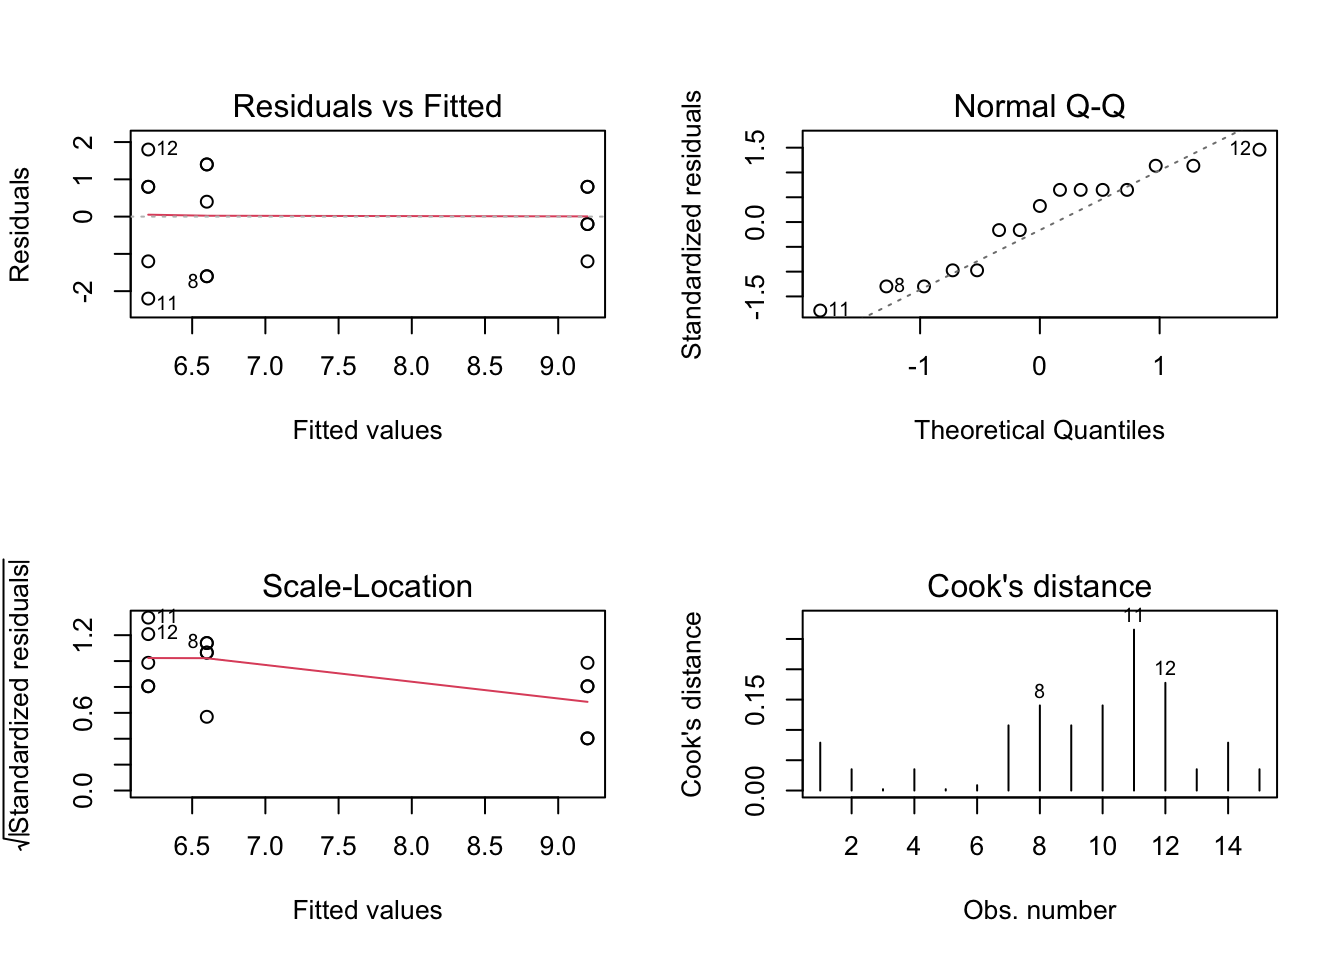
\includegraphics{_main_files/figure-latex/unnamed-chunk-114-2.pdf}

\begin{Shaded}
\begin{Highlighting}[]
\CommentTok{\# pela função anova}
\KeywordTok{anova}\NormalTok{(}\KeywordTok{lm}\NormalTok{(x }\OperatorTok{\textasciitilde{}}\StringTok{ }\NormalTok{g))}
\end{Highlighting}
\end{Shaded}

\begin{verbatim}
## Analysis of Variance Table
## 
## Response: x
##           Df Sum Sq Mean Sq F value Pr(>F)   
## g          2   26.5    13.3    6.98 0.0097 **
## Residuals 12   22.8     1.9                  
## ---
## Signif. codes:  0 '***' 0.001 '**' 0.01 '*' 0.05 '.' 0.1 ' ' 1
\end{verbatim}

\begin{Shaded}
\begin{Highlighting}[]
\CommentTok{\# pela função car::Anova}
\NormalTok{car}\OperatorTok{::}\KeywordTok{Anova}\NormalTok{(}\KeywordTok{lm}\NormalTok{(x }\OperatorTok{\textasciitilde{}}\StringTok{ }\NormalTok{g))}
\end{Highlighting}
\end{Shaded}

\begin{verbatim}
## Anova Table (Type II tests)
## 
## Response: x
##           Sum Sq Df F value Pr(>F)   
## g           26.5  2    6.98 0.0097 **
## Residuals   22.8 12                  
## ---
## Signif. codes:  0 '***' 0.001 '**' 0.01 '*' 0.05 '.' 0.1 ' ' 1
\end{verbatim}

\begin{Shaded}
\begin{Highlighting}[]
\CommentTok{\# pela função lm}
\KeywordTok{summary}\NormalTok{(}\KeywordTok{lm}\NormalTok{(x }\OperatorTok{\textasciitilde{}}\StringTok{ }\NormalTok{g))}
\end{Highlighting}
\end{Shaded}

\begin{verbatim}
## 
## Call:
## lm(formula = x ~ g)
## 
## Residuals:
##    Min     1Q Median     3Q    Max 
##   -2.2   -1.2    0.4    0.8    1.8 
## 
## Coefficients:
##             Estimate Std. Error t value Pr(>|t|)    
## (Intercept)    9.200      0.616   14.92  4.1e-09 ***
## g2            -2.600      0.872   -2.98   0.0114 *  
## g3            -3.000      0.872   -3.44   0.0049 ** 
## ---
## Signif. codes:  0 '***' 0.001 '**' 0.01 '*' 0.05 '.' 0.1 ' ' 1
## 
## Residual standard error: 1.38 on 12 degrees of freedom
## Multiple R-squared:  0.538,  Adjusted R-squared:  0.461 
## F-statistic: 6.98 on 2 and 12 DF,  p-value: 0.00974
\end{verbatim}

\begin{Shaded}
\begin{Highlighting}[]
\CommentTok{\# Post{-}hoc}
\NormalTok{stats}\OperatorTok{::}\KeywordTok{TukeyHSD}\NormalTok{(anova1)}
\end{Highlighting}
\end{Shaded}

\begin{verbatim}
##   Tukey multiple comparisons of means
##     95% family-wise confidence level
## 
## Fit: aov(formula = x ~ g)
## 
## $g
##     diff   lwr    upr p adj
## 2-1 -2.6 -4.93 -0.274 0.029
## 3-1 -3.0 -5.33 -0.674 0.013
## 3-2 -0.4 -2.73  1.926 0.891
\end{verbatim}

\begin{Shaded}
\begin{Highlighting}[]
\NormalTok{rstatix}\OperatorTok{::}\KeywordTok{tukey\_hsd}\NormalTok{(anova1)}
\end{Highlighting}
\end{Shaded}

\begin{verbatim}
## # A tibble: 3 x 9
##   term  group1 group2 null.value estimate conf.low conf.high  p.adj p.adj.signif
## * <chr> <chr>  <chr>       <dbl>    <dbl>    <dbl>     <dbl>  <dbl> <chr>       
## 1 g     1      2               0    -2.60    -4.93    -0.274 0.0286 *           
## 2 g     1      3               0    -3       -5.33    -0.674 0.0126 *           
## 3 g     2      3               0    -0.4     -2.73     1.93  0.891  ns
\end{verbatim}

\begin{exercise}
\protect\hypertarget{exr:anova-hot-dog}{}{\label{exr:anova-hot-dog} }(Adaptado de (DeGroot and Schervish \protect\hyperlink{ref-degroot2012probability}{2012}, 754)) Moore e McCabe (1999) descrevem dados coletados em \emph{Consumer Reports} (junho de 1986, pp.~364-67). Os dados incluem (entre outras coisas) calorias conteúdo de 63 marcas de salsichas de cachorros-quentes conforme tabela a seguir. A salsichas vêm em quatro variedades: carne bovina, carne (?), aves e especialidades. É interessante saber se, e em que medida, as diferentes variedades diferem em seus conteúdos calóricos. Realize o procedimento de análise de variância e post hoc, indicando se há diferença significativa entre os grupos.

\textbf{Carne bovina} 186, 181, 176, 149, 184, 190, 158, 139, 175, 148, 152, 111, 141, 153, 190, 157, 131, 149, 135, 132\\
\textbf{Carne} 173, 191, 182, 190, 172, 147, 146, 139, 175, 136, 179, 153,107, 195, 135, 140, 138\\
\textbf{Aves} 129, 132, 102, 106, 94, 102, 87, 99, 107, 113, 135, 142, 86, 143, 152, 146, 144\\
\textbf{Especialidades} 155, 170, 114, 191, 162, 146, 140, 187, 180
\end{exercise}

\begin{Shaded}
\begin{Highlighting}[]
\CommentTok{\# Dica}
\NormalTok{g \textless{}{-}}\StringTok{ }\KeywordTok{as.factor}\NormalTok{(}\KeywordTok{rep}\NormalTok{(}\DecValTok{1}\OperatorTok{:}\DecValTok{4}\NormalTok{, }\DataTypeTok{times=}\KeywordTok{c}\NormalTok{(}\DecValTok{20}\NormalTok{,}\DecValTok{17}\NormalTok{,}\DecValTok{17}\NormalTok{,}\DecValTok{9}\NormalTok{)))}
\end{Highlighting}
\end{Shaded}

\hypertarget{testes-nuxe3o-paramuxe9tricos-univariados}{%
\subsection{Testes Não Paramétricos Univariados}\label{testes-nuxe3o-paramuxe9tricos-univariados}}

\hypertarget{teste-13---teste-dos-postos-sinalizados-de-wilcoxon-para-uma-amostra}{%
\subsubsection*{TESTE 13 - Teste dos postos sinalizados de Wilcoxon para uma amostra}\label{teste-13---teste-dos-postos-sinalizados-de-wilcoxon-para-uma-amostra}}
\addcontentsline{toc}{subsubsection}{TESTE 13 - Teste dos postos sinalizados de Wilcoxon para uma amostra}

\textbf{Hipótese avaliada}\\
Uma amostra de \(n\) sujeitos (ou objetos) vem de uma população em que a mediana \(\theta\) é igual a um valor especificado?

\textbf{Suposições}\\
S1. Cada amostra foi selecionada aleatoriamente da população que representa;\\
S2. As pontuações originais obtidas para cada um dos sujeitos/objetos são quantitativas;\\
S3. A distribuição da população subjacente é simétrica.

\textbf{Testes relacionados}\\
TESTE 1 - Teste \(z\) para média de uma amostra\\
TESTE 2 - Teste \(t\) para média de uma amostra

Para testar a simetria foi considerada a função \texttt{symmetry\_test} do pacote \texttt{symmetry}. Segundo (Milošević and Obradović \protect\hyperlink{ref-milosevic2018comparison}{2018}, 4), entre os testes originalmente destinados a testar simetria em torno de uma média desconhecida, o mais famoso é o teste clássico \(\sqrt{b_1}\), baseado no coeficiente de assimetria da amostra, com estatística de teste \(\sqrt{b_1} = m_3/s^3\) onde \(m_3\) é o terceiro momento central da amostra conforme numerador da Eq. \eqref{eq:ass1} e \(s\) é o desvio padrão amostral conforme Eq. \eqref{eq:dp-am}.

\begin{Shaded}
\begin{Highlighting}[]
\CommentTok{\# dados}
\KeywordTok{set.seed}\NormalTok{(}\DecValTok{456}\NormalTok{); z \textless{}{-}}\StringTok{ }\KeywordTok{rnorm}\NormalTok{(}\DecValTok{100}\NormalTok{) }\CommentTok{\# N(0,1)}
\CommentTok{\# verificando suposição S3 (simetria)}
\KeywordTok{library}\NormalTok{(symmetry)}
\KeywordTok{set.seed}\NormalTok{(}\DecValTok{111}\NormalTok{); }\KeywordTok{symmetry\_test}\NormalTok{(z, }\StringTok{\textquotesingle{}B1\textquotesingle{}}\NormalTok{)  }\CommentTok{\# √b1}
\end{Highlighting}
\end{Shaded}

\begin{verbatim}
## 
##  Symmetry test
##  Null hypothesis: Data is symmetric
## 
## data:  z
## B1 = -2e-04, B = 1000, p-value = 1
## sample estimates:
##    mu 
## 0.121
\end{verbatim}

\begin{Shaded}
\begin{Highlighting}[]
\CommentTok{\# teste de Wilcoxon}
\KeywordTok{wilcox.test}\NormalTok{(z, }\DataTypeTok{mu =} \DecValTok{0}\NormalTok{) }\CommentTok{\# mediana 0}
\end{Highlighting}
\end{Shaded}

\begin{verbatim}
## 
##  Wilcoxon signed rank test with continuity correction
## 
## data:  z
## V = 2851, p-value = 0.3
## alternative hypothesis: true location is not equal to 0
\end{verbatim}

\begin{Shaded}
\begin{Highlighting}[]
\KeywordTok{wilcox.test}\NormalTok{(z, }\DataTypeTok{mu =} \DecValTok{1}\NormalTok{) }\CommentTok{\# mediana 1}
\end{Highlighting}
\end{Shaded}

\begin{verbatim}
## 
##  Wilcoxon signed rank test with continuity correction
## 
## data:  z
## V = 563, p-value = 2e-11
## alternative hypothesis: true location is not equal to 1
\end{verbatim}

\hypertarget{teste-14---teste-de-aderuxeancia-de-shapiro-wilk-para-uma-amostra}{%
\subsubsection*{TESTE 14 - Teste de aderência de Shapiro-Wilk para uma amostra}\label{teste-14---teste-de-aderuxeancia-de-shapiro-wilk-para-uma-amostra}}
\addcontentsline{toc}{subsubsection}{TESTE 14 - Teste de aderência de Shapiro-Wilk para uma amostra}

\textbf{Hipótese avaliada}\\
Os dados têm distribuição normal?

\textbf{Suposições}\\
S1. Cada amostra foi selecionada aleatoriamente da população que representa;\\
S2. A escala de mensuração é quantitativa.

\begin{Shaded}
\begin{Highlighting}[]
\KeywordTok{set.seed}\NormalTok{(}\DecValTok{8765}\NormalTok{); z \textless{}{-}}\StringTok{ }\KeywordTok{rnorm}\NormalTok{(}\DecValTok{100}\NormalTok{, }\DataTypeTok{mean =} \DecValTok{5}\NormalTok{, }\DataTypeTok{sd =} \DecValTok{3}\NormalTok{)}
\KeywordTok{shapiro.test}\NormalTok{(z)}
\end{Highlighting}
\end{Shaded}

\begin{verbatim}
## 
##  Shapiro-Wilk normality test
## 
## data:  z
## W = 1, p-value = 0.3
\end{verbatim}

\begin{Shaded}
\begin{Highlighting}[]
\KeywordTok{set.seed}\NormalTok{(}\DecValTok{7654}\NormalTok{); u \textless{}{-}}\StringTok{ }\KeywordTok{runif}\NormalTok{(}\DecValTok{100}\NormalTok{, }\DataTypeTok{min =} \DecValTok{4}\NormalTok{, }\DataTypeTok{max =} \DecValTok{6}\NormalTok{)}
\KeywordTok{shapiro.test}\NormalTok{(u)}
\end{Highlighting}
\end{Shaded}

\begin{verbatim}
## 
##  Shapiro-Wilk normality test
## 
## data:  u
## W = 1, p-value = 0.002
\end{verbatim}

\hypertarget{testes-nuxe3o-paramuxe9tricos-bivariados}{%
\subsection{Testes Não Paramétricos Bivariados}\label{testes-nuxe3o-paramuxe9tricos-bivariados}}

\hypertarget{teste-15---teste-de-kolmogorov-smirnov-para-duas-amostras-independentes}{%
\subsubsection*{TESTE 15 - Teste de Kolmogorov-Smirnov para duas amostras independentes}\label{teste-15---teste-de-kolmogorov-smirnov-para-duas-amostras-independentes}}
\addcontentsline{toc}{subsubsection}{TESTE 15 - Teste de Kolmogorov-Smirnov para duas amostras independentes}

\textbf{Hipótese avaliada}\\
Duas amostras independentes representam duas populações distintas?

\textbf{Suposições}\\
S1. Cada amostra foi selecionada aleatoriamente da população que representa;\\
S2. A escala de mensuração é pelo menos ordinal.

\begin{Shaded}
\begin{Highlighting}[]
\CommentTok{\# veja ?ks.test}
\KeywordTok{set.seed}\NormalTok{(}\DecValTok{99}\NormalTok{); x \textless{}{-}}\StringTok{ }\KeywordTok{rnorm}\NormalTok{(}\DecValTok{50}\NormalTok{)}
\KeywordTok{set.seed}\NormalTok{(}\DecValTok{88}\NormalTok{); y \textless{}{-}}\StringTok{ }\KeywordTok{runif}\NormalTok{(}\DecValTok{30}\NormalTok{)}
\KeywordTok{ks.test}\NormalTok{(x, y)}
\end{Highlighting}
\end{Shaded}

\begin{verbatim}
## 
##  Two-sample Kolmogorov-Smirnov test
## 
## data:  x and y
## D = 0.5, p-value = 4e-05
## alternative hypothesis: two-sided
\end{verbatim}

\begin{Shaded}
\begin{Highlighting}[]
\KeywordTok{set.seed}\NormalTok{(}\DecValTok{77}\NormalTok{); z \textless{}{-}}\StringTok{ }\KeywordTok{runif}\NormalTok{(}\DecValTok{30}\NormalTok{)}
\KeywordTok{ks.test}\NormalTok{(x, z)}
\end{Highlighting}
\end{Shaded}

\begin{verbatim}
## 
##  Two-sample Kolmogorov-Smirnov test
## 
## data:  x and z
## D = 0.5, p-value = 1e-05
## alternative hypothesis: two-sided
\end{verbatim}

\begin{Shaded}
\begin{Highlighting}[]
\KeywordTok{ks.test}\NormalTok{(y, z)}
\end{Highlighting}
\end{Shaded}

\begin{verbatim}
## 
##  Two-sample Kolmogorov-Smirnov test
## 
## data:  y and z
## D = 0.2, p-value = 0.8
## alternative hypothesis: two-sided
\end{verbatim}

\hypertarget{teste-16---teste-dos-postos-de-mann-whitney-para-amostras-independentes}{%
\subsubsection*{TESTE 16 - Teste dos postos de Mann-Whitney para amostras independentes}\label{teste-16---teste-dos-postos-de-mann-whitney-para-amostras-independentes}}
\addcontentsline{toc}{subsubsection}{TESTE 16 - Teste dos postos de Mann-Whitney para amostras independentes}

\textbf{Hipótese avaliada}\\
Duas amostras independentes representam duas populações com medianas diferentes?

\textbf{Suposições}\\
S1. Cada amostra foi selecionada aleatoriamente da população que representa;\\
S2. As duas amostras são independentes entre si;\\
S3. Os dados são ordinais ou quantitativos;\\
S4. As distribuições de onde as amostras foram retiradas possuem mesma forma.

\textbf{Testes relacionados}\\
TESTE 7 - Teste \(z\) para médias de duas amostras independentes\\
TESTE 8 - Teste \(t\) para médias de duas amostras independentes

\begin{example}
\protect\hypertarget{exm:mw1}{}{\label{exm:mw1} }(Adaptado de (Sheskin \protect\hyperlink{ref-sheskin2011handbook}{2011}, 532)) Para avaliar a eficácia de um novo medicamento antidepressivo, dez pacientes com depressão clínica são aleatoriamente designados para um dos dois grupos. Cinco pacientes são atribuídos ao Grupo 1, onde é administrado o antidepressivo por um período de seis meses. Os outros cinco pacientes são atribuídos ao Grupo 2, que recebe um placebo durante o mesmo período de seis meses. Suponha que, antes de introduzir os tratamentos experimentais, o experimentador confirmou que o nível de depressão nos dois grupos era igual. Após seis meses, todos os dez sujeitos são avaliados por um psiquiatra (que é cego em relação à condição experimental do sujeito) quanto ao nível de depressão. As classificações de depressão do psiquiatra para os cinco sujeitos em cada grupo seguem (quanto mais alta a classificação, mais deprimido é o sujeito): Grupo 1: 11, 1,0, 2, 0; Grupo 2: 11, 11, 5, 8, 4. Os dados indicam que o antidepressivo é eficaz?

\[\left\{ 
    \begin{array}{l}
      H_0: \theta_1 \ge \theta_2 \equiv \theta_1 - \theta_2 \ge 0 \; \text{(tratamento igual ou menos eficaz que o placebo)} \\
      H_1: \theta_1 < \theta_2 \equiv \theta_1 - \theta_2 < 0 \; \text{(tratamento mais eficaz que o placebo)} \\ \end{array} \right. \]
\end{example}

\begin{Shaded}
\begin{Highlighting}[]
\NormalTok{x \textless{}{-}}\StringTok{ }\KeywordTok{c}\NormalTok{(}\DecValTok{11}\NormalTok{,}\DecValTok{1}\NormalTok{,}\DecValTok{0}\NormalTok{,}\DecValTok{2}\NormalTok{,}\DecValTok{0}\NormalTok{)}
\NormalTok{y \textless{}{-}}\StringTok{ }\KeywordTok{c}\NormalTok{(}\DecValTok{11}\NormalTok{,}\DecValTok{11}\NormalTok{,}\DecValTok{5}\NormalTok{,}\DecValTok{8}\NormalTok{,}\DecValTok{4}\NormalTok{)}
\KeywordTok{median}\NormalTok{(x); }\KeywordTok{median}\NormalTok{(y)}
\end{Highlighting}
\end{Shaded}

\begin{verbatim}
## [1] 1
\end{verbatim}

\begin{verbatim}
## [1] 8
\end{verbatim}

\begin{Shaded}
\begin{Highlighting}[]
\CommentTok{\# avaliando S4}
\KeywordTok{ks.test}\NormalTok{(x,y)}
\end{Highlighting}
\end{Shaded}

\begin{verbatim}
## Warning in ks.test(x, y): cannot compute exact p-value with ties
\end{verbatim}

\begin{verbatim}
## 
##  Two-sample Kolmogorov-Smirnov test
## 
## data:  x and y
## D = 0.8, p-value = 0.08
## alternative hypothesis: two-sided
\end{verbatim}

\begin{Shaded}
\begin{Highlighting}[]
\KeywordTok{wilcox.test}\NormalTok{(x, y, }\DataTypeTok{alternative  =} \StringTok{\textquotesingle{}less\textquotesingle{}}\NormalTok{)}
\end{Highlighting}
\end{Shaded}

\begin{verbatim}
## Warning in wilcox.test.default(x, y, alternative = "less"): cannot compute exact p-value with ties
\end{verbatim}

\begin{verbatim}
## 
##  Wilcoxon rank sum test with continuity correction
## 
## data:  x and y
## W = 4, p-value = 0.04
## alternative hypothesis: true location shift is less than 0
\end{verbatim}

\hypertarget{teste-17---teste-dos-postos-de-wilcoxon-para-amostras-dependentespareadas}{%
\subsubsection*{TESTE 17 - Teste dos postos de Wilcoxon para amostras dependentes/pareadas}\label{teste-17---teste-dos-postos-de-wilcoxon-para-amostras-dependentespareadas}}
\addcontentsline{toc}{subsubsection}{TESTE 17 - Teste dos postos de Wilcoxon para amostras dependentes/pareadas}

\textbf{Hipótese avaliada}\\
Duas amostras dependentes representam duas populações distintas?

\textbf{Suposições}\\
S1. Cada amostra foi selecionada aleatoriamente da população que representa;\\
S2. As pontuações originais obtidas para cada um dos sujeitos/objetos são quantitativas;\\
S3. A distribuição dos escores de diferença nas populações representadas pelas duas amostras é simétrica em relação à mediana da população de escores de diferença.

\textbf{Testes relacionados}\\
TESTE 9 - Teste \(t\) para médias de duas amostras dependentes/pareadas.

Assim como no \emph{teste dos postos sinalizados de Wilcoxon para uma amostra} (TESTE 14), para testar a simetria foi considerada a estatística \(\sqrt{b_1}\) da função \texttt{symmetry::symmetry\_test}.

\begin{Shaded}
\begin{Highlighting}[]
\CommentTok{\# dados}
\NormalTok{x \textless{}{-}}\StringTok{ }\KeywordTok{c}\NormalTok{(}\FloatTok{1.83}\NormalTok{,  }\FloatTok{0.50}\NormalTok{,  }\FloatTok{1.62}\NormalTok{,  }\FloatTok{2.48}\NormalTok{, }\FloatTok{1.68}\NormalTok{, }\FloatTok{1.88}\NormalTok{, }\FloatTok{1.55}\NormalTok{, }\FloatTok{3.06}\NormalTok{, }\FloatTok{1.30}\NormalTok{)}
\NormalTok{y \textless{}{-}}\StringTok{ }\KeywordTok{c}\NormalTok{(}\FloatTok{0.878}\NormalTok{, }\FloatTok{0.647}\NormalTok{, }\FloatTok{0.598}\NormalTok{, }\FloatTok{2.05}\NormalTok{, }\FloatTok{1.06}\NormalTok{, }\FloatTok{1.29}\NormalTok{, }\FloatTok{1.06}\NormalTok{, }\FloatTok{3.14}\NormalTok{, }\FloatTok{1.29}\NormalTok{)}
\KeywordTok{median}\NormalTok{(x}\OperatorTok{{-}}\NormalTok{y)}
\end{Highlighting}
\end{Shaded}

\begin{verbatim}
## [1] 0.49
\end{verbatim}

\begin{Shaded}
\begin{Highlighting}[]
\CommentTok{\# verificando suposição S3 (simetria da diferença em relação à mediana)}
\KeywordTok{set.seed}\NormalTok{(}\DecValTok{111}\NormalTok{); symmetry}\OperatorTok{::}\KeywordTok{symmetry\_test}\NormalTok{(x}\OperatorTok{{-}}\NormalTok{y, }\StringTok{\textquotesingle{}B1\textquotesingle{}}\NormalTok{, }\DataTypeTok{mu =} \KeywordTok{median}\NormalTok{(x}\OperatorTok{{-}}\NormalTok{y))  }\CommentTok{\# √b1}
\end{Highlighting}
\end{Shaded}

\begin{verbatim}
## 
##  Symmetry test
##  Null hypothesis: Data is symmetric around 0.49
## 
## data:  x - y
## B1 = -0.07, B = 1000, p-value = 0.9
\end{verbatim}

\begin{Shaded}
\begin{Highlighting}[]
\CommentTok{\# teste de Wilcoxon para amostras pareadas}
\KeywordTok{wilcox.test}\NormalTok{(x, y, }\DataTypeTok{paired =} \OtherTok{TRUE}\NormalTok{, }\DataTypeTok{alternative =} \StringTok{\textquotesingle{}greater\textquotesingle{}}\NormalTok{)}
\end{Highlighting}
\end{Shaded}

\begin{verbatim}
## 
##  Wilcoxon signed rank exact test
## 
## data:  x and y
## V = 40, p-value = 0.02
## alternative hypothesis: true location shift is greater than 0
\end{verbatim}

\hypertarget{teste-18---teste-de-mcnemar-para-amostras-dependentespareadas}{%
\subsubsection*{TESTE 18 - Teste de McNemar para amostras dependentes/pareadas}\label{teste-18---teste-de-mcnemar-para-amostras-dependentespareadas}}
\addcontentsline{toc}{subsubsection}{TESTE 18 - Teste de McNemar para amostras dependentes/pareadas}

\textbf{Hipótese avaliada}\\
Duas amostras dependentes representam duas populações distintas?

\textbf{Suposições}\\
S1. Cada amostra foi selecionada aleatoriamente da população que representa;\\
S2. As variáveis são binárias e categóricas (ordinais ou nominais);\\
S3. Cada um dos \(n\) sujeitos (ou \(n\) pares de sujeitos combinados) contribui com duas pontuações na variável dependente.

\textbf{Estatística do teste}\\
Sob \(H_0:\pi_{12}=\pi_{21}\),
\begin{equation} 
\chi_{teste}^2 = \frac{(n_{12}-n_{21})^2}{n_{12}+n_{21}} \sim \chi^2(1)
\label{eq:mcnemar}
\end{equation}
onde \(n_{12}\) indica o número de elementos da linha 1, coluna 2 da tabela e \(n_{21}\) indica o número de elementos da linha 2, coluna e \(\chi^2(1)\) indica a distribuição qui-quadrado com 1 grau de liberdade.

\textbf{Estatística do teste com correção de continuidade}\\
Sob \(H_0:\pi_{12}=\pi_{21}\),
\begin{equation} 
\chi_{teste}^2 = \frac{(|n_{12}-n_{21}|-1)^2}{n_{12}+n_{21}} \sim \chi^2(1)
\label{eq:mcnemar-corr}
\end{equation}

\textbf{Valor-p}\\
Sob \(H_0: \pi_{12}=\pi_{21}\),
\begin{equation}
\text{Valor-p} = Pr(\chi^2 \ge \chi_{teste}^2).
\label{eq:mcnemar-bi}
\end{equation}

\begin{example}
\protect\hypertarget{exm:presidential}{}{\label{exm:presidential} }(Exemplo da documentação de \texttt{mcnemar.test}) A aprovação do desempenho do Presidente no cargo foi realizado em duas pesquisas, com um mês de intervalo, para uma amostra aleatória de 1.600 americanos em idade de votar. Os dados indicam uma mudança de percepção em relação às duas pesquisas?
\end{example}

\begin{Shaded}
\begin{Highlighting}[]
\CommentTok{\# dados}
\NormalTok{dat \textless{}{-}}\StringTok{ }\KeywordTok{matrix}\NormalTok{(}\KeywordTok{c}\NormalTok{(}\DecValTok{794}\NormalTok{, }\DecValTok{86}\NormalTok{, }\DecValTok{150}\NormalTok{, }\DecValTok{570}\NormalTok{), }\DataTypeTok{nrow =} \DecValTok{2}\NormalTok{,}
              \DataTypeTok{dimnames =} \KeywordTok{list}\NormalTok{(}\StringTok{\textquotesingle{}1ª pesquisa\textquotesingle{}}\NormalTok{ =}\StringTok{ }\KeywordTok{c}\NormalTok{(}\StringTok{\textquotesingle{}Aprova\textquotesingle{}}\NormalTok{, }\StringTok{\textquotesingle{}Desaprova\textquotesingle{}}\NormalTok{),}
                              \StringTok{\textquotesingle{} 2ª pesquisa\textquotesingle{}}\NormalTok{ =}\StringTok{ }\KeywordTok{c}\NormalTok{(}\StringTok{\textquotesingle{}Aprova\textquotesingle{}}\NormalTok{, }\StringTok{\textquotesingle{}Desaprova\textquotesingle{}}\NormalTok{)))}
\NormalTok{dat}
\end{Highlighting}
\end{Shaded}

\begin{verbatim}
##             2ª pesquisa
## 1ª pesquisa Aprova Desaprova
##   Aprova       794       150
##   Desaprova     86       570
\end{verbatim}

\begin{Shaded}
\begin{Highlighting}[]
\CommentTok{\# usando a estatística do teste sem correção}
\NormalTok{(qui \textless{}{-}}\StringTok{ }\NormalTok{(dat[}\DecValTok{1}\NormalTok{,}\DecValTok{2}\NormalTok{]}\OperatorTok{{-}}\NormalTok{dat[}\DecValTok{2}\NormalTok{,}\DecValTok{1}\NormalTok{])}\OperatorTok{\^{}}\DecValTok{2}\OperatorTok{/}\NormalTok{(dat[}\DecValTok{1}\NormalTok{,}\DecValTok{2}\NormalTok{]}\OperatorTok{+}\NormalTok{dat[}\DecValTok{2}\NormalTok{,}\DecValTok{1}\NormalTok{]))}
\end{Highlighting}
\end{Shaded}

\begin{verbatim}
## [1] 17.4
\end{verbatim}

\begin{Shaded}
\begin{Highlighting}[]
\CommentTok{\# valor{-}p}
\DecValTok{1}\OperatorTok{{-}}\KeywordTok{pchisq}\NormalTok{(qui,}\DecValTok{1}\NormalTok{)}
\end{Highlighting}
\end{Shaded}

\begin{verbatim}
## [1] 3.1e-05
\end{verbatim}

\begin{Shaded}
\begin{Highlighting}[]
\CommentTok{\# teste via mcnemar.test}
\KeywordTok{mcnemar.test}\NormalTok{(dat, }\DataTypeTok{correct =}\NormalTok{ F)}
\end{Highlighting}
\end{Shaded}

\begin{verbatim}
## 
##  McNemar's Chi-squared test
## 
## data:  dat
## McNemar's chi-squared = 17, df = 1, p-value = 3e-05
\end{verbatim}

\begin{Shaded}
\begin{Highlighting}[]
\CommentTok{\# usando a estatística do teste com correção}
\NormalTok{(qui.c \textless{}{-}}\StringTok{ }\NormalTok{(}\KeywordTok{abs}\NormalTok{(dat[}\DecValTok{1}\NormalTok{,}\DecValTok{2}\NormalTok{]}\OperatorTok{{-}}\NormalTok{dat[}\DecValTok{2}\NormalTok{,}\DecValTok{1}\NormalTok{])}\OperatorTok{{-}}\DecValTok{1}\NormalTok{)}\OperatorTok{\^{}}\DecValTok{2}\OperatorTok{/}\NormalTok{(dat[}\DecValTok{1}\NormalTok{,}\DecValTok{2}\NormalTok{]}\OperatorTok{+}\NormalTok{dat[}\DecValTok{2}\NormalTok{,}\DecValTok{1}\NormalTok{]))}
\end{Highlighting}
\end{Shaded}

\begin{verbatim}
## [1] 16.8
\end{verbatim}

\begin{Shaded}
\begin{Highlighting}[]
\CommentTok{\# valor{-}p}
\DecValTok{1}\OperatorTok{{-}}\KeywordTok{pchisq}\NormalTok{(qui.c,}\DecValTok{1}\NormalTok{)}
\end{Highlighting}
\end{Shaded}

\begin{verbatim}
## [1] 4.11e-05
\end{verbatim}

\begin{Shaded}
\begin{Highlighting}[]
\CommentTok{\# teste via mcnemar.test}
\KeywordTok{mcnemar.test}\NormalTok{(dat, }\DataTypeTok{correct =}\NormalTok{ T)}
\end{Highlighting}
\end{Shaded}

\begin{verbatim}
## 
##  McNemar's Chi-squared test with continuity correction
## 
## data:  dat
## McNemar's chi-squared = 17, df = 1, p-value = 4e-05
\end{verbatim}

\begin{exercise}
\protect\hypertarget{exr:tv-animal}{}{\label{exr:tv-animal} }Um pesquisador conduz um estudo para investigar se uma série semanal de televisão altamente crítica quanto ao uso de animais em pesquisas médicas influencia a opinião pública. Cem sujeitos selecionados aleatoriamente são avaliados por um teste para determinar sua atitude em relação ao uso de animais em pesquisas médicas. Com base em suas respostas, os sujeitos são então categorizados como pró-pesquisa com animais ou anti-pesquisa com animais. Após o pré-teste, todos os sujeitos são orientados a assistir à série de televisão (com duração de dois meses). Na conclusão da série, a atitude de cada sujeito em relação à pesquisa animal é reavaliada. Os resultados do estudo estão resumidos na tabela a seguir. Os dados indicam que uma mudança de atitude em relação à pesquisa com animais ocorreu depois que os participantes assistiram à série de televisão?\\
Resolva utilizando as estatísticas com e sem correção de continuidade, realizando os cálculos e também aplicando a função \texttt{mcnemar.test}.

\begin{longtable}[]{@{}lccc@{}}
\toprule
& Pós-teste & &\tabularnewline
\midrule
\endhead
\textbf{Pré-teste} & \textbf{Anti} & \textbf{Pró} & \textbf{Total}\tabularnewline
\textbf{Anti} & 10 & 13 & \textbf{23}\tabularnewline
\textbf{Pró} & 41 & 36 & \textbf{77}\tabularnewline
\textbf{Total} & \textbf{51} & \textbf{49} & \textbf{100}\tabularnewline
\bottomrule
\end{longtable}
\end{exercise}

\hypertarget{testes-nuxe3o-paramuxe9tricos-multivariados}{%
\subsection{Testes Não Paramétricos Multivariados}\label{testes-nuxe3o-paramuxe9tricos-multivariados}}

\hypertarget{teste-19---teste-de-kruskal-wallis-de-um-fator-entre-sujeitos}{%
\subsubsection*{TESTE 19 - Teste de Kruskal-Wallis de um fator entre sujeitos}\label{teste-19---teste-de-kruskal-wallis-de-um-fator-entre-sujeitos}}
\addcontentsline{toc}{subsubsection}{TESTE 19 - Teste de Kruskal-Wallis de um fator entre sujeitos}

\textbf{Hipótese avaliada}\\
Em um conjunto de \(k \ge 2\) grupos independentes, há pelo menos dois com medianas distintas?

\textbf{Suposições}\\
S1. Cada amostra foi selecionada aleatoriamente da população que representa;\\
S2. As \(k\) amostras são independentes umas das outras;\\
S3. A variável dependente (que é subsequentemente classificada) é uma variável aleatória contínua.\\
S4. As distribuições subjacentes das quais as amostras são derivadas possuem a mesma forma, não obrigatoriamente normais.

\textbf{Testes relacionados}\\
TESTE 12 - Análise de Variância (ANOVA) de um fator entre sujeitos

\begin{example}
\protect\hypertarget{exm:kw-entre-suj}{}{\label{exm:kw-entre-suj} }Pode-se resolver o Exemplo \ref{exm:anova-entre-suj} através do teste de Kruskal-Wallis.
\end{example}

\begin{Shaded}
\begin{Highlighting}[]
\CommentTok{\# dados}
\NormalTok{x \textless{}{-}}\StringTok{ }\KeywordTok{c}\NormalTok{(}\DecValTok{8}\NormalTok{,}\DecValTok{10}\NormalTok{,}\DecValTok{9}\NormalTok{,}\DecValTok{10}\NormalTok{,}\DecValTok{9}\NormalTok{, }\DecValTok{7}\NormalTok{,}\DecValTok{8}\NormalTok{,}\DecValTok{5}\NormalTok{,}\DecValTok{8}\NormalTok{,}\DecValTok{5}\NormalTok{, }\DecValTok{4}\NormalTok{,}\DecValTok{8}\NormalTok{,}\DecValTok{7}\NormalTok{,}\DecValTok{5}\NormalTok{,}\DecValTok{7}\NormalTok{)}
\NormalTok{g \textless{}{-}}\StringTok{ }\KeywordTok{as.factor}\NormalTok{(}\KeywordTok{rep}\NormalTok{(}\DecValTok{1}\OperatorTok{:}\DecValTok{3}\NormalTok{, }\DataTypeTok{each =} \DecValTok{5}\NormalTok{))}
\NormalTok{(k \textless{}{-}}\StringTok{ }\KeywordTok{length}\NormalTok{(}\KeywordTok{unique}\NormalTok{(g))) }\CommentTok{\# número de grupos}
\end{Highlighting}
\end{Shaded}

\begin{verbatim}
## [1] 3
\end{verbatim}

\begin{Shaded}
\begin{Highlighting}[]
\KeywordTok{boxplot}\NormalTok{(x }\OperatorTok{\textasciitilde{}}\StringTok{ }\NormalTok{g)}
\end{Highlighting}
\end{Shaded}

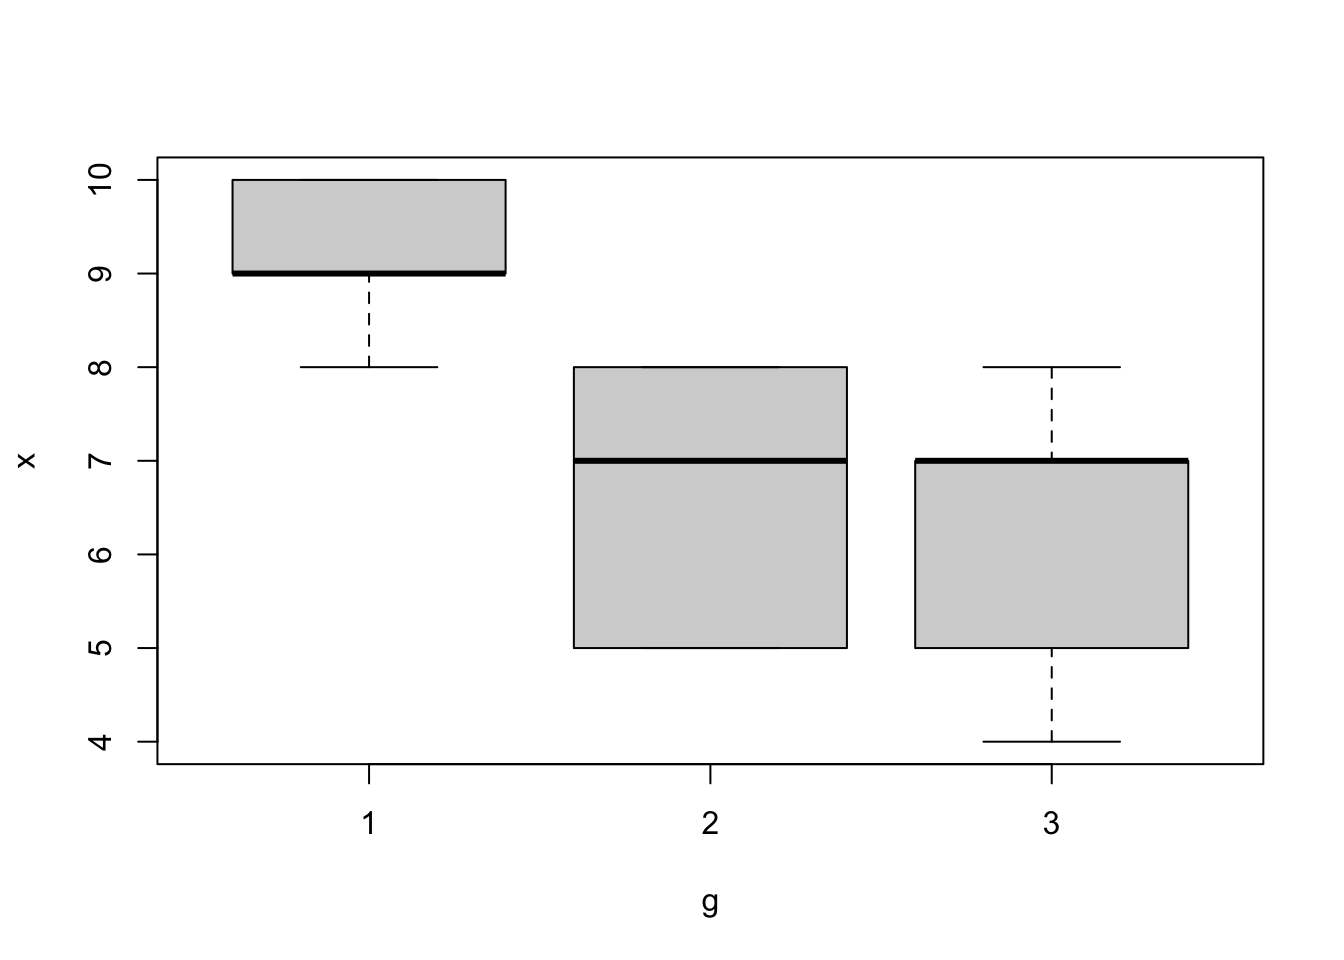
\includegraphics{_main_files/figure-latex/unnamed-chunk-122-1.pdf}

\begin{Shaded}
\begin{Highlighting}[]
\CommentTok{\# validando suposição S4 via TESTE 19 {-} teste K{-}S para duas amostras independentes}
\KeywordTok{ks.test}\NormalTok{(x[}\DecValTok{1}\OperatorTok{:}\DecValTok{5}\NormalTok{], x[}\DecValTok{6}\OperatorTok{:}\DecValTok{10}\NormalTok{])}
\end{Highlighting}
\end{Shaded}

\begin{verbatim}
## Warning in ks.test(x[1:5], x[6:10]): cannot compute exact p-value with ties
\end{verbatim}

\begin{verbatim}
## 
##  Two-sample Kolmogorov-Smirnov test
## 
## data:  x[1:5] and x[6:10]
## D = 0.8, p-value = 0.08
## alternative hypothesis: two-sided
\end{verbatim}

\begin{Shaded}
\begin{Highlighting}[]
\KeywordTok{ks.test}\NormalTok{(x[}\DecValTok{1}\OperatorTok{:}\DecValTok{5}\NormalTok{], x[}\DecValTok{11}\OperatorTok{:}\DecValTok{15}\NormalTok{])}
\end{Highlighting}
\end{Shaded}

\begin{verbatim}
## Warning in ks.test(x[1:5], x[11:15]): cannot compute exact p-value with ties
\end{verbatim}

\begin{verbatim}
## 
##  Two-sample Kolmogorov-Smirnov test
## 
## data:  x[1:5] and x[11:15]
## D = 0.8, p-value = 0.08
## alternative hypothesis: two-sided
\end{verbatim}

\begin{Shaded}
\begin{Highlighting}[]
\KeywordTok{ks.test}\NormalTok{(x[}\DecValTok{6}\OperatorTok{:}\DecValTok{10}\NormalTok{], x[}\DecValTok{11}\OperatorTok{:}\DecValTok{15}\NormalTok{])}
\end{Highlighting}
\end{Shaded}

\begin{verbatim}
## Warning in ks.test(x[6:10], x[11:15]): cannot compute exact p-value with ties
\end{verbatim}

\begin{verbatim}
## 
##  Two-sample Kolmogorov-Smirnov test
## 
## data:  x[6:10] and x[11:15]
## D = 0.2, p-value = 1
## alternative hypothesis: two-sided
\end{verbatim}

\begin{Shaded}
\begin{Highlighting}[]
\CommentTok{\# aplicando o teste de Kruskal{-}Wallis}
\KeywordTok{kruskal.test}\NormalTok{(x,g)}
\end{Highlighting}
\end{Shaded}

\begin{verbatim}
## 
##  Kruskal-Wallis rank sum test
## 
## data:  x and g
## Kruskal-Wallis chi-squared = 9, df = 2, p-value = 0.01
\end{verbatim}

\begin{Shaded}
\begin{Highlighting}[]
\CommentTok{\# comparando com a ANOVA}
\KeywordTok{summary}\NormalTok{(}\KeywordTok{aov}\NormalTok{(x }\OperatorTok{\textasciitilde{}}\StringTok{ }\NormalTok{g))}
\end{Highlighting}
\end{Shaded}

\begin{verbatim}
##             Df Sum Sq Mean Sq F value Pr(>F)   
## g            2   26.5    13.3    6.98 0.0097 **
## Residuals   12   22.8     1.9                  
## ---
## Signif. codes:  0 '***' 0.001 '**' 0.01 '*' 0.05 '.' 0.1 ' ' 1
\end{verbatim}

\begin{exercise}
\protect\hypertarget{exr:kw-hot-dog}{}{\label{exr:kw-hot-dog} }Refaça o exercício \ref{exr:anova-hot-dog} aplicando o teste de Kruskal-Wallis.
\end{exercise}

\hypertarget{exercuxedcios}{%
\section{Exercícios}\label{exercuxedcios}}

\begin{enumerate}
\def\labelenumi{\arabic{enumi}.}
\tightlist
\item
  O diâmetro nominal de uma amostra de 20 peças, cujos resultados estão em cm foram:
\end{enumerate}

\begin{longtable}[]{@{}cccccccccc@{}}
\toprule
41 & 50 & 52 & 49 & 49 & 54 & 50 & 47 & 52 & 49\tabularnewline
\midrule
\endhead
50 & 52 & 50 & 47 & 49 & 51 & 46 & 50 & 49 & 50\tabularnewline
\bottomrule
\end{longtable}

\textbf{\texttt{(a)}} Suponha inicialmente que o diâmetro populacional possui variância de \(\sigma^2=2\) cm\(^2\). Teste a hipótese de que a média seja diferente de 50cm com \(\alpha=0.05\).\\
\textbf{\texttt{(b)}} Faça o mesmo teste para a média, mas agora desconhecendo a variância, novamente com \(\alpha=0.05\).

\begin{enumerate}
\def\labelenumi{\arabic{enumi}.}
\setcounter{enumi}{1}
\item
  Um processo deveria produzir mesas com 0.85m de altura. O engenheiro desconfia que as mesas que estão sendo produzidas são menores que o especificado. Uma amostra de 8 mesas foi coletada e indicou média 0.847m. Sabendo que o desvio padrão é \(\sigma=0.01\)m, obtenha o valor-p e teste a hipótese do engenheiro usando um nível de significância de 3\%.
\item
  As condições de mortalidade de uma região são tais que a proporção de nascidos que sobrevivem até 60 anos é de 0.6. Testar essa hipótese ao nível de 5\% se em 1000 nascimentos amostrados aleatoriamente, verificou-se 530 sobreviventes até 60 anos.
\item
  A experiência tem comprovado que mais de 40\% dos estudantes são reprovados em uma prova de certa matéria. Se 45 de 90 estudantes amostrados fossem reprovados, o que se pode concluir a respeito desta afirmação. Obtenha o valor-p e teste esta hipótese ao nível de significância de 4\%.
\item
  Funcionários de uma grande firma de contabilidade alegam que seu salário médio anual é menor que o de seu concorrente que é de R\$ 45,000, sabe-se também que o desvio padrão de ambas as empresas são iguais a R\$ 5,200. Uma amostra de 30 contadores da empresa gera um salário médio de R\$ 43,500. Teste a alegação dos empregados ao nível de significância de 1\%.
\item
  Certo fabricante de parafusos anuncia que 90\% do seu produto não apresenta qualquer tipo de defeito. Um comprador acredita que a percentagem de parafusos perfeitos é diferente da anunciada pelo fabricante. Para verificar tal hipótese, examinou 400 parafusos, verificando que 344 eram perfeitos. Com \(\alpha=2\%\), realize o teste correspondente.
\item
  Certa organização médica afirma que um novo medicamento é de qualidade superior ao até então existente, que é 80\% eficaz na cura de determinada doença. Examinada uma amostra de 300 pessoas que sofriam da doença, constatou-se que 249 ficaram curadas com o novo medicamento. Obtenha o valor-p e teste a afirmação da organização ao nível de significância de 5\%.
\item
  Como responsável pelas compras em um mercado, suponha que você tome uma amostra aleatória de 32 latas de um certo produto. O peso líquido encontrado foi de 15.95g e o desvio padrão de 0.15g. Foi afirmado que o peso médio desse produto é 16.0g. Pode-se considerar essa afirmação verdadeira ao nível de significância de 5\%? Usando a tabela \(t\), o valor-p estaria entre quais valores? E usando o software, qual o valor mais preciso?
\item
  Uma certa agência bancária afirma que o tempo médio de espera na fila é de 15 minutos. Entretanto, os clientes estão revoltados com a demora no atendimento e dizem que a afirmação não é verdadeira, ou seja, o tempo de espera é superior a 15 min. Para poder argumentar contra o banco, os clientes realizam uma amostra com 200 pessoas, anotando o tempo até o atendimento. O resultado foi um tempo médio de espera de 19 min e variância de 49 min\(^2\). Ao nível de significância de 5\%, quem tem razão?
\item
  A empresa XYZ possui o seguinte critério para aceitar ou rejeitar um lote de matéria prima (aço). Se o nível de pureza do aço for superior a 90.0 o lote é aceito, caso contrário é rejeitado. Um lote chega à empresa e cinco amostras são analisadas. Os níveis de pureza encontrados estão apresentados a seguir. O lote deve ser aceito, utilizando nível de significância de 1\%? Formule as hipóteses da forma que achar mais adequada.
\end{enumerate}

\begin{longtable}[]{@{}cllll@{}}
\toprule
89.8 & 89.0 & 92.2 & 92.5 & 93.0\tabularnewline
\midrule
\endhead
\bottomrule
\end{longtable}

\begin{enumerate}
\def\labelenumi{\arabic{enumi}.}
\setcounter{enumi}{10}
\tightlist
\item
  Um estudo do tempo médio de adaptação dos funcionários está sendo realizado num grande complexo industrial. Supõe-se que os homens tenham um tempo de adaptação menor do que as mulheres. Sabendo que numa amostra de 31 homens o tempo médio de adaptação foi de 3.2 anos e o desvio padrão de 1.3 ano. Numa amostra de 41 mulheres o tempo médio de adaptação foi de 3.7 anos e desvio de 0.8 ano.
\end{enumerate}

\textbf{\texttt{(a)}} É possível obter o p-valor exato?\\
\textbf{\texttt{(b)}} Teste essa hipótese com \(\alpha=0.05\).

\begin{enumerate}
\def\labelenumi{\arabic{enumi}.}
\setcounter{enumi}{11}
\item
  Um estudo está sendo realiza com com 121 crianças de escolas da rede pública e 121 crianças da rede particular. O estudo consiste da realização de um jogo onde é anotado o tempo de realização até a obtenção da resposta correta. Nas crianças da rede pública o tempo médio foi de 12 minutos, com um desvio padrão de 8 minutos. Na rede particular o tempo médio foi de 13 minutos, com um desvio de 5 minutos. Teste ao nível de significância de 5\% se há diferença entre os tempos de realização do jogo entre alunos da rede pública e particular.
\item
  A empresa Chips está oferecendo a suas melhores equipes de vendas, prêmios em forma de viagens. A empresa quer saber se realmente os prêmios estão incentivando seus vendedores. Segue amostra de 8 equipes de vendas com o volume de vendas em ABR e MAI (considere que os meses de abril e maio são historicamente semelhantes).
\end{enumerate}

\begin{longtable}[]{@{}lcccccccc@{}}
\toprule
Equipe & A & B & C & D & E & F & G & H\tabularnewline
\midrule
\endhead
Abril (antes da promoção) & 15.7 & 18.8 & 19.7 & 16.8 & 59.1 & 2.7 & 45.1 & 3.1\tabularnewline
Maio (após a promoção) & 17.0 & 18.7 & 21.5 & 17.6 & 65.2 & 2.5 & 47.2 & 3.7\tabularnewline
\bottomrule
\end{longtable}

Verifique se a campanha publicitária pode ser considerada eficiente ao nível de 1\%. Qual o valor-p?

\begin{enumerate}
\def\labelenumi{\arabic{enumi}.}
\setcounter{enumi}{13}
\tightlist
\item
  Por determinação do Governo Federal, as indústrias refinadoras de Sal devem misturar 1mg (0.001g) de iodo para cada grama de sal. Suspeita-se que a marca SALMOURA DOS PAMPAS não esteja cumprindo a especificação. Na amostra abaixo foram observados os resultados (em mg). Qual sua decisão com \(\alpha=0.05\)?
\end{enumerate}

\begin{longtable}[]{@{}ccccc@{}}
\toprule
1.2 & 1.1 & 1.01 & 0.9 & 0.8\tabularnewline
\midrule
\endhead
\bottomrule
\end{longtable}

\begin{enumerate}
\def\labelenumi{\arabic{enumi}.}
\setcounter{enumi}{14}
\tightlist
\item
  As lojas GASTÃO e PRAQUETÁ pertencem a um mesmo grupo. Suspeita-se que o nível de satisfação médio dos clientes seja diferente de uma loja para outra. Os dados a seguir são baseados numa pesquisa feita por telefone que utilizou uma escala de 0 (pior avaliação) até 100 (melhor avaliação). Compare o nível de satisfação das lojas utilizando um nível de significância de 5\%.
\end{enumerate}

\begin{longtable}[]{@{}cc@{}}
\toprule
GASTÃO & PRAQUETÁ\tabularnewline
\midrule
\endhead
\(n=180\) & \(n=160\)\tabularnewline
\(\bar{x}_G=85.0\) & \(\bar{x}_P=77.0\)\tabularnewline
\(s_G=18.0\) & \(s_P=15.0\)\tabularnewline
\bottomrule
\end{longtable}

\begin{enumerate}
\def\labelenumi{\arabic{enumi}.}
\setcounter{enumi}{15}
\tightlist
\item
  A frequência crítica de oscilação (fco) é a frequência mais alta (em ciclos/s) na qual uma pessoa pode detectar a oscilação em uma fonte de luz oscilante. Em frequências acima de fco, a fonte de luz parece ser contínua, embora na verdade esteja oscilante. Uma investigação realizada para verificar se a fco média real depende da cor da íris, gerou os dados abaixo. Investigue as diferenças entre as cores em relação à fco média, com \(\alpha=5\%\).
\end{enumerate}

\begin{longtable}[]{@{}ccccccccc@{}}
\toprule
Cor & Dados & & & & & & &\tabularnewline
\midrule
\endhead
Marrom & 26.8 & 27.9 & 23.7 & 25.0 & 26.3 & 24.8 & 24.5 & 25.7\tabularnewline
Verde & 26.4 & 24.2 & 28.0 & 26.9 & 29.1 & & &\tabularnewline
Azul & 25.7 & 27.2 & 29.9 & 28.5 & 29.4 & 28.3 & &\tabularnewline
\bottomrule
\end{longtable}

\hypertarget{inferencia-bayesiana}{%
\chapter{Inferência Bayesiana}\label{inferencia-bayesiana}}

O paradigma da \emph{inferência bayesiana} tem suas origens no artigo póstumo de (Bayes \protect\hyperlink{ref-bayes1763essay}{1763}), comunicado por seu amigo Richard Price. As derivações das ideias de Bayes são extensas e profundas matemática e filosoficamente, discutidas por grandes nomes da Ciência em incontáveis livros, artigos e compilações ao longo destes mais de 250 anos. Desta forma entende-se que a melhor abordagem para este material é indicar o estado-da-arte da aplicação bayesiana considerando referências consagradas disponíveis online ou na bilbioteca da PUCRS.

\begin{exercise}
\protect\hypertarget{exr:unnamed-chunk-123}{}{\label{exr:unnamed-chunk-123} }Assita aos vídeos \href{https://www.youtube.com/watch?v=R13BD8qKeTg\&vl=en}{The Bayesian Trap} e \href{https://www.youtube.com/watch?v=HZGCoVF3YvM}{Bayes theorem}. Lembre que você pode ativar a legenda (botão CC) e alterar a língua nas configurações (ícone de engrenagem \textgreater{} legendas). \(\\\)
\end{exercise}

Um dos principais motivos dos avanços recentes na pesquisa em estatística bayesiana é a crescente facilidade no acesso a recursos computacionais, tanto de hardware quanto de software. Na linguagem R existem muitas bibliotecas para aplicação bayesiana. O \href{https://cran.r-project.org/web/views/}{CRAN Task View}\footnote{Segundo a documentação oficial do R, os \emph{CRAN Task Views} (`Visualizadores de Tarefa da Rede Abrangente de Arquivos R', em tradução livre) têm como objetivo fornecer alguma orientação sobre quais pacotes no CRAN são relevantes para tarefas relacionadas a um determinado tópico. Eles fornecem uma breve visão geral dos pacotes incluídos têm como objetivo ter um foco nítido para que seja suficientemente claro quais pacotes devem ser incluídos (ou excluídos) - e não têm a intenção de endossar os ``melhores'' pacotes para uma determinada tarefa.} de \href{https://cran.r-project.org/view=Bayesian}{inferência bayesiana} fornece um compêndio atualizado dos pacotes relacionados ao assunto.

\hypertarget{princuxedpios-de-verossimilhanuxe7a-suficiuxeancia-e-condicionalidade}{%
\section{Princípios de verossimilhança, suficiência e condicionalidade}\label{princuxedpios-de-verossimilhanuxe7a-suficiuxeancia-e-condicionalidade}}

\begin{itemize}
\tightlist
\item
  Seção 1.6 de (Paulino, Turkman, and Murteira \protect\hyperlink{ref-paulino2003estatistica}{2003})\\
\item
  Seções 3.3 e 3.4 de (Press \protect\hyperlink{ref-press2003subjective}{2003}) (Princípio da verossimilhança)\\
\item
  Os fundamentos são discutidos por (Birnbaum \protect\hyperlink{ref-birnbaum1962foundations}{1962}), (Savage et al. \protect\hyperlink{ref-savage1962foundations}{1962}) e (Wechsler, Pereira, and Marques \protect\hyperlink{ref-wechsler2008birnbaum}{2008})
\end{itemize}

Informalmente, o \emph{princípio da verossimilhança} admite que se dois decisores possuem o mesmo grau de conhecimento e a mesma informação sobre \(\theta\), ambos devem decidir exatamente da mesma forma a respeito de \(\theta\). (Berger \protect\hyperlink{ref-berger1985statistical}{1985}, 28)\footnote{``\emph{The Likelihood Principle. In making inferences or decisions about \(\theta\) after x is observed, all relevant experimental information is contained in the likelihood function for the observed x. Furthermore, two likelihood functions contain the same information about \(\theta\) if they are proportional to each other (as functions of \(\theta\)).}'' (Berger \protect\hyperlink{ref-berger1985statistical}{1985}, 28)} define da seguinte forma:

\begin{quote}
\textbf{Princípio da verossimilhança} Ao fazer inferências ou decisões sobre \(\theta\) após observar \(x\), todas as informações experimentais relevantes estão contidas na função de verossimilhança para o \(x\) observado. Além disso, duas funções de verossimilhança contêm as mesmas informações sobre \(\theta\) se forem proporcionais entre si (como funções de \(\theta\)).
\end{quote}

\begin{example}
\protect\hypertarget{exm:pv1}{}{\label{exm:pv1} }(Princípio da Verossimilhança 1, adaptado de (Paulino, Turkman, and Murteira \protect\hyperlink{ref-paulino2003estatistica}{2003})) Considere uma sucessão de lançamentos de uma moeda, independentes e condicionados por \(\theta\), a probabilidade de sair `cara'. Suponha que seja obtido o resultado \[x  =  \lbrace H,T,H,H,T,T,H,T,T,T  \rbrace,\] onde \(H\): `cara' e \(T\): `coroa'\footnote{Do Inglês \emph{Head} (cara) e \emph{Tail} (coroa).}. Este resultado poderia ser obtido de diversos processos experimentais ou regras de parada, como\\
- realizar 10 lançamentos, fixados a priori\\
- lançar a moeda até aparecerem 6 `coroas'\\
- lançar a moeda até aparecerem 3 `coroas' consecutivas\\
- lançar a moeda até o jogador ficar saturado, tendo a saturação ocorrido no 10º lançamento

Em qualquer caso a (função de) verossimilhança é proporcional a \(\theta^4 \left( 1 - \theta \right)^6\), i.e., a amostra informa quatro sucessos (caras) e seis fracassos (coroas). Assim, adotando-se o princípio da verossimilhança, toda a informação que \(x\) pode fornecer sobre \(\theta\) encontra-se nesta expressão. Saber qual dos quatro processos experimentais foi utilizado (cada um com um espaço amostral diferente) ou saber qual foi a regra de parada adotada nada tem a acrescentar. Note que a possibilidade de o experimentador parar por seu arbítrio ao considerar o resultado \(x\) satisfatório, em nada altera a opinião sobre \(\theta\). \(\\\)
\end{example}

\begin{example}
\protect\hypertarget{exm:pv2}{}{\label{exm:pv2} }(Princípio da Verossimilhança 2, adaptado de (Lindley and Phillips \protect\hyperlink{ref-lindley1976inference}{1976}) por (Paulino, Turkman, and Murteira \protect\hyperlink{ref-paulino2003estatistica}{2003})) Suponha que deseja-se testar a hipótese \(H_0 : \theta \le 1/2\) contra \(H_1 : \theta > 1/2\). São contemplados dois processos experimentais:

\begin{itemize}
\tightlist
\item
  \(E_1\): lançar a moeda \(n=12\) vezes;\\
\item
  \(E_2\): lançar a moeda até que apareçam \(k=3\) `caras'
\end{itemize}

Admita que o resultado observado nas duas experiências foi \(x=9\) `coroas' (portanto 3 `caras'), que é uma particular realização da variável aleatória \(X\), que designa o número total de `coroas' dos experimentos \(E_1\) e \(E_2\). Para um clássico o nível crítico (ou valor-\(p\), a probabilidade de obter \(X \ge 9\)) da hipótese \(H_0 : \theta = 1/2\) difere nos dois casos.

No caso \(E_1\), \(X\) tem distribuição binomial -- \(X \sim \mathcal{B} \left( 12, \theta \right)\) -- cujo nível crítico é

\begin{equation}
Pr\left( X \geq 9 \bigg\rvert \theta = \dfrac{1}{2} \right) = \binom {12}{9}  \left(  \frac{1}{2} \right) ^{12} + \binom {12}{10} \left(  \frac{1}{2} \right) ^{12} + \binom {12}{11}  \left(  \frac{1}{2} \right) ^{12} + \binom {12}{12} \left( \frac{1}{2} \right) ^{12} \approx 0.0730. \nonumber
\label{eq:pvalue-binom}
\end{equation}

No caso \(E_2\), \(X\) tem distribuição binomial negativa -- \(X \sim \mathcal{BN} \left( 3, 1-\theta \right)\) -- que tem nível crítico

\begin{equation}
Pr\left( X \geq 9 \bigg\rvert \theta = \dfrac{1}{2} \right) = \binom {11}{9}  \left(  \frac{1}{2} \right) ^{12} + \binom {12}{10} \left(  \frac{1}{2} \right) ^{13} +\binom {13}{11}  \left(  \frac{1}{2} \right) ^{14} + \cdots \approx 0.0327. \nonumber
\label{eq:pvalue-nbinom}
\end{equation}

Logo, se for adotado um limiar de significância de \(5 \%\), \(H_0\) é rejeitada no caso \(E_2\) e não rejeitada em \(E_1\). Assumindo o princípio da verossimilhança, as conclusões devem ser idênticas nos dois casos. Em ambos a (função de) verossimilhança é proporcional a \(\theta^9 \left( 1 - \theta \right)^3\). De fato, as verossimilhanças em \(E_1\) e \(E_2\) são

\[L_1 \left( \theta \right| x = 9 ) = \binom {12}{9} \theta^{9} \left( 1-\theta \right) ^{3} = 220 \; \theta^{9} \left( 1-\theta \right)^{3} \propto \theta^{9} \left( 1-\theta \right)^{3}\]

\bigskip

\[L_2 \left( \theta \right| x = 9 ) = \binom {11}{9} \theta^{9} \left( 1-\theta \right) ^{3} = 55 \; \theta^{9} \left( 1-\theta \right)^{3} \propto \theta^{9} \left( 1-\theta \right)^{3}\]
\end{example}

\hypertarget{distribuiuxe7uxe3o-a-priori}{%
\section{Distribuição a priori}\label{distribuiuxe7uxe3o-a-priori}}

\begin{itemize}
\tightlist
\item
  Fundamentos abordados no Capítulo 2 de (Paulino, Turkman, and Murteira \protect\hyperlink{ref-paulino2003estatistica}{2003}) e no Capítulo 5 de (Press \protect\hyperlink{ref-press2003subjective}{2003})\\
\item
  (Morris, Oakley, and Crowe \protect\hyperlink{ref-morris2014web}{2014}) apresentam uma ferramenta baseada na web para obter distribuições de probabilidade de especialistas
\end{itemize}

\hypertarget{estimauxe7uxe3o-pontual-1}{%
\section{Estimação Pontual}\label{estimauxe7uxe3o-pontual-1}}

\begin{itemize}
\tightlist
\item
  Seções 8.2 e 8.3 de (Press \protect\hyperlink{ref-press2003subjective}{2003})\\
\item
  Seção 3.2 de (Paulino, Turkman, and Murteira \protect\hyperlink{ref-paulino2003estatistica}{2003})\\
\end{itemize}

\hypertarget{estimauxe7uxe3o-por-intervaloregiuxf5es-de-credibilidade}{%
\section{(Estimação por) Intervalo/Regiões de Credibilidade}\label{estimauxe7uxe3o-por-intervaloregiuxf5es-de-credibilidade}}

\begin{itemize}
\tightlist
\item
  Seção 8.4 de (Press \protect\hyperlink{ref-press2003subjective}{2003})\\
\item
  Seção 3.3 de (Paulino, Turkman, and Murteira \protect\hyperlink{ref-paulino2003estatistica}{2003})\\
\end{itemize}

\hypertarget{estimauxe7uxe3o-por-teste-de-hipuxf3teses-1}{%
\section{(Estimação por) Teste de Hipóteses}\label{estimauxe7uxe3o-por-teste-de-hipuxf3teses-1}}

\begin{itemize}
\tightlist
\item
  Capítulo 9 de (Press \protect\hyperlink{ref-press2003subjective}{2003})\\
\item
  Seção 3.4 de (Paulino, Turkman, and Murteira \protect\hyperlink{ref-paulino2003estatistica}{2003})
\end{itemize}

\hypertarget{fatores-de-bayes}{%
\subsection{Fatores de Bayes}\label{fatores-de-bayes}}

\begin{itemize}
\tightlist
\item
  (Kass and Raftery \protect\hyperlink{ref-kass1995bayes}{1995})\\
\item
  Seção 9.5.1 de (Press \protect\hyperlink{ref-press2003subjective}{2003})\\
\item
  Seção 3.4.1 de (Paulino, Turkman, and Murteira \protect\hyperlink{ref-paulino2003estatistica}{2003})
\end{itemize}

\hypertarget{fbst---full-bayesian-significance-test}{%
\subsection{\texorpdfstring{FBST - \emph{Full Bayesian Significance Test}}{FBST - Full Bayesian Significance Test}}\label{fbst---full-bayesian-significance-test}}

\begin{itemize}
\tightlist
\item
  Proposta de (Pereira and Stern \protect\hyperlink{ref-pereira1999evidence}{1999}) para testar hipóteses precisas (\emph{sharp hypotheses})\\
\item
  Amplamente revisado em (Pereira et al. \protect\hyperlink{ref-pereira2008can}{2008}) e (Pereira and Stern \protect\hyperlink{ref-pereira2020evalue}{2020})
\end{itemize}

\hypertarget{modelos-lineares}{%
\chapter{Modelos Lineares}\label{modelos-lineares}}

A classe de \emph{Modelos Lineares} atende a uma ampla gama de problemas aplicados, apresentada em profundidade por (Neter et al. \protect\hyperlink{ref-neter2005applied}{2005}). Para uma introdução à classe de \emph{Modelos Lineares Generalizados} recomenda-se (McCullagh and Nelder \protect\hyperlink{ref-mccullagh1989generalized}{1989}).

\hypertarget{correlacao}{%
\section{Correlação}\label{correlacao}}

\hypertarget{regressuxe3o-linear-simples}{%
\section{Regressão Linear Simples}\label{regressuxe3o-linear-simples}}

\hypertarget{modelo}{%
\subsection{Modelo}\label{modelo}}

O modelo de \emph{Regressão Linear Simples} universal/populacional é construído, pela abordagem clássica, com todos os \(N\) pares ordenados do universo, e pode ser descrito pela relação a seguir.

\begin{equation}
Y_i = \beta_0 + \beta_1 X_i + \varepsilon_i,
\label{eq:rls}
\end{equation}
onde \(\varepsilon_i \sim \mathcal{N}(0,\sigma_{\varepsilon})\).

Na maioria dos casos práticos trabalha-se com amostras, sendo necessário estimar os valores de \(\beta_0\) e \(\beta_1\). O método dos \emph{mínimos quadrados (ordinários)} é utilizado para calcular estas estimativas. O princípio do método é minimizar a soma de quadrado dos erros, i.e.,
\begin{equation}
minimizar \sum_{i=1}^n \varepsilon_{i}^{2}.
\label{eq:mqo}
\end{equation}

\hypertarget{estimativas-dos-paruxe2metros}{%
\subsection{Estimativas dos parâmetros}\label{estimativas-dos-paruxe2metros}}

Basicamente utiliza-se \(\varepsilon_{i} = Y_{i} - \beta_0 - \beta_1 X_i\) da Eq. \eqref{eq:rls} e deriva-se (parcialmente) em relação a \(\beta_0\) e \(\beta_1\), fazendo cada uma das derivadas parciais igual a zero. Para maiores detalhes recomenda-se (DeGroot and Schervish \protect\hyperlink{ref-degroot2012probability}{2012}). As estimativas por mínimos quadrados são enfim dadas por
\begin{equation}
\hat{\beta}_1 = \frac{n \sum{x_i y_i} - \sum{x_i} \sum{y_i}}{n \sum{x_i^2} - (\sum{x_i})^2} 
\label{eq:beta1}
\end{equation}
e
\begin{equation}
\hat{\beta}_0 = \bar{y} - \hat{\beta}_1 \bar{x}.
\label{eq:beta0}
\end{equation}

\hypertarget{anuxe1lise-de-diagnuxf3stico}{%
\subsection{Análise de diagnóstico}\label{anuxe1lise-de-diagnuxf3stico}}

\hypertarget{teste-para-beta_0}{%
\subsubsection*{\texorpdfstring{Teste para \(\beta_0\)}{Teste para \textbackslash beta\_0}}\label{teste-para-beta_0}}
\addcontentsline{toc}{subsubsection}{Teste para \(\beta_0\)}

As hipóteses usuais do teste para \(\beta_0\) são \(H_0: \beta_0 = 0\) \emph{vs} \(H_1: \beta_0 \ne 0\). Sob \(H_0\)
\begin{equation}
T_0 = \frac{\hat{\beta}_0}{ep(\hat{\beta}_0)} \sim t_{n-2},
(\#eq:teste_b0)
\end{equation}
onde
\begin{equation}
ep(\hat{\beta}_0) = \sqrt{\hat{\sigma}^2 \left[ \frac{1}{n} + \frac{\bar{x}^2}{S_{xx}} \right] } = \sqrt{\frac{\sum_{i=i}^n (y_i - \hat{y}_i)^2}{n-2} \left[ \frac{1}{n} + \frac{\bar{x}^2}{\sum_{i=i}^n (x_i - \bar{x})^2} \right] }.
(\#eq:ep_b0)
\end{equation}

\hypertarget{teste-para-beta_1}{%
\subsubsection*{\texorpdfstring{Teste para \(\beta_1\)}{Teste para \textbackslash beta\_1}}\label{teste-para-beta_1}}
\addcontentsline{toc}{subsubsection}{Teste para \(\beta_1\)}

O teste para \(\beta_1\) é fundamental na análise de diagnóstico. É com ele que decide-se a respeito da presença ou ausência de relação linear entre \(X\) e \(Y\). As hipóteses usuais do teste para \(\beta_1\) são \(H_0: \beta_1 = 0\) \emph{vs} \(H_1: \beta_1 \ne 0\). Sob \(H_0\)
\begin{equation}
T_1 = \frac{\hat{\beta}_1}{ep(\hat{\beta}_1)} \sim t_{n-2},
\label{eq:t1}
\end{equation}
onde
\begin{equation}
ep(\hat{\beta}_1) = \sqrt{\frac{\hat{\sigma}^2}{S_{xx}}} = \sqrt{\frac{\sum_{i=i}^n (y_i - \hat{y}_i)^2 / (n-2)}{\sum_{i=i}^n (x_i - \bar{x})^2} }.
(\#eq:ep_t1)
\end{equation}

\hypertarget{modelo-rpo}{%
\subsection{Modelo RPO}\label{modelo-rpo}}

Um modelo na forma da Eq. \eqref{eq:rls0} é chamado \emph{regressão pela origem} pelo fato de a reta ajustada passar pelo ponto \((0,0)\), a \emph{origem} do plano cartesiano.
\begin{equation}
Y_i = \beta_1 X_i + \varepsilon_i,
\label{eq:rls0}
\end{equation}
onde \(\varepsilon_i \sim \mathcal{N}(0,\sigma_{\varepsilon})\). A estimativa do parâmetro \(\beta_1\) é dada por
\begin{equation}
\hat{\beta}_1 = \frac{\sum{x_i y_i} }{\sum{x_i^2} }.
(\#eq:beta1_rpo)
\end{equation}

\hypertarget{teste-para-beta_1-do-modelo-rpo}{%
\subsubsection*{\texorpdfstring{Teste para \(\beta_1\) do modelo RPO}{Teste para \textbackslash beta\_1 do modelo RPO}}\label{teste-para-beta_1-do-modelo-rpo}}
\addcontentsline{toc}{subsubsection}{Teste para \(\beta_1\) do modelo RPO}

\begin{equation}
T_1^{RPO} = \frac{\hat{\beta}_1}{ep(\hat{\beta}_1)} \sim t_{n-1},
(\#eq:teste_beta1_rpo)
\end{equation}
onde
\begin{equation}
ep(\hat{\beta}_1) = \sqrt{\frac{\hat{\sigma}^2}{S_{xx}}} = \sqrt{\frac{\sum_{i=i}^n (y_i - \hat{y}_i)^2 / (n-1)}{\sum_{i=i}^n x_{i}^{2} } }.
(\#eq:ep_beta1_rpo)
\end{equation}

\begin{example}
\protect\hypertarget{exm:unnamed-chunk-125}{}{\label{exm:unnamed-chunk-125} }O dono de um bar decidiu modelar o número de garrafas de bebidas vendidas em seu estabelecimento (\(Y\)) em função da temperatura máxima do dia (\(X\)).
\end{example}

\begin{Shaded}
\begin{Highlighting}[]
\NormalTok{x \textless{}{-}}\StringTok{ }\KeywordTok{read.table}\NormalTok{(}\StringTok{\textquotesingle{}http://www.filipezabala.com/data/drinks.txt\textquotesingle{}}\NormalTok{, }\DataTypeTok{header =}\NormalTok{ T, }\DataTypeTok{sep =} \StringTok{\textquotesingle{}}\CharTok{\textbackslash{}t}\StringTok{\textquotesingle{}}\NormalTok{)}
\KeywordTok{dim}\NormalTok{(x)  }\CommentTok{\# dimensão de x}
\end{Highlighting}
\end{Shaded}

\begin{verbatim}
## [1] 30  2
\end{verbatim}

\begin{Shaded}
\begin{Highlighting}[]
\KeywordTok{head}\NormalTok{(x) }\CommentTok{\# cabeçalho de x}
\end{Highlighting}
\end{Shaded}

\begin{verbatim}
##   temp gar
## 1 29.5 145
## 2 31.3 170
## 3 34.7 167
## 4 40.4 244
## 5 28.4 159
## 6 40.3 195
\end{verbatim}

\begin{Shaded}
\begin{Highlighting}[]
\NormalTok{fit \textless{}{-}}\StringTok{ }\KeywordTok{lm}\NormalTok{(gar }\OperatorTok{\textasciitilde{}}\StringTok{ }\NormalTok{temp, }\DataTypeTok{data =}\NormalTok{ x)       }\CommentTok{\# regressão linear simples}
\KeywordTok{summary}\NormalTok{(fit)}
\end{Highlighting}
\end{Shaded}

\begin{verbatim}
## 
## Call:
## lm(formula = gar ~ temp, data = x)
## 
## Residuals:
##    Min     1Q Median     3Q    Max 
## -44.16  -8.96   3.58  10.81  33.60 
## 
## Coefficients:
##             Estimate Std. Error t value Pr(>|t|)    
## (Intercept)  -19.334     22.944   -0.84     0.41    
## temp           5.920      0.674    8.78  1.6e-09 ***
## ---
## Signif. codes:  0 '***' 0.001 '**' 0.01 '*' 0.05 '.' 0.1 ' ' 1
## 
## Residual standard error: 18.3 on 28 degrees of freedom
## Multiple R-squared:  0.734,  Adjusted R-squared:  0.724 
## F-statistic: 77.1 on 1 and 28 DF,  p-value: 1.57e-09
\end{verbatim}

\begin{Shaded}
\begin{Highlighting}[]
\NormalTok{fit0 \textless{}{-}}\StringTok{ }\KeywordTok{lm}\NormalTok{(gar }\OperatorTok{\textasciitilde{}}\StringTok{ }\NormalTok{temp }\OperatorTok{{-}}\StringTok{ }\DecValTok{1}\NormalTok{, }\DataTypeTok{data =}\NormalTok{ x)  }\CommentTok{\# regressão pela origem}
\KeywordTok{summary}\NormalTok{(fit0)}
\end{Highlighting}
\end{Shaded}

\begin{verbatim}
## 
## Call:
## lm(formula = gar ~ temp - 1, data = x)
## 
## Residuals:
##    Min     1Q Median     3Q    Max 
## -45.78 -11.26   3.53  12.01  30.29 
## 
## Coefficients:
##      Estimate Std. Error t value Pr(>|t|)    
## temp   5.3582     0.0975      55   <2e-16 ***
## ---
## Signif. codes:  0 '***' 0.001 '**' 0.01 '*' 0.05 '.' 0.1 ' ' 1
## 
## Residual standard error: 18.2 on 29 degrees of freedom
## Multiple R-squared:  0.99,   Adjusted R-squared:  0.99 
## F-statistic: 3.02e+03 on 1 and 29 DF,  p-value: <2e-16
\end{verbatim}

\begin{exercise}
\protect\hypertarget{exr:unnamed-chunk-127}{}{\label{exr:unnamed-chunk-127} }Considere o Exemplo 5.1.\\
(a) Indique os valores de \(n\) e \(p\).\\
(b) No modelo de regressão linear simples atribuído a \texttt{fit}, indique os números das equações para o cálculo das medidas \texttt{Estimate}, \texttt{Std.\ Error} e \texttt{t\ value}.\\
(c) Utilizado a linguagem R, aplique as equações indicadas no item (b) de forma a obter os valores indicados em \texttt{summary(fit)}.\\
(d) No modelo de regressão pela origem atribuído a \texttt{fit0}, indique os números das equações para o cálculo das medidas \texttt{Estimate}, \texttt{Std.\ Error} e \texttt{t\ value}.\\
(e) Utilizado a linguagem R, aplique as equações indicadas no item (d) de forma a obter os valores indicados em \texttt{summary(fit0)}.\\
(f) Qual o modelo mais indicado segundo a sua análise? Justifique.
\end{exercise}

\hypertarget{regressuxe3o-linear-muxfaltipla}{%
\section{Regressão Linear Múltipla}\label{regressuxe3o-linear-muxfaltipla}}

O modelo de \emph{regressão linear múltipla} universal/populacional é construído, pela abordagem clássica, com todos os \(N\) pares ordenados do universo, e pode ser descrito pela relação a seguir.

\begin{equation}
Y_i = \beta_0 + \beta_1 X_{i1} + \beta_2 X_{i2} + \cdots + \beta_p X_{ip} + \varepsilon_i,
\label{eq:rlm}
\end{equation}
\(\varepsilon_i \sim \mathcal{N}(0,\sigma_{\varepsilon})\). Por ter dimensionalidade \(p\) usualmente utiliza-se notação matricial na forma

\begin{equation}
\boldsymbol{Y} = \boldsymbol{X} \boldsymbol{\beta} + \boldsymbol{\varepsilon},
\label{eq:rlm2}
\end{equation}
onde \(\boldsymbol{Y} = \begin{bmatrix} Y_1 \\ Y_2 \\ \vdots \\ Y_n \end{bmatrix}\), \(\boldsymbol{X} = \begin{bmatrix} 1 & X_{11} & X_{12} & \cdots & X_{1p} \\ 1 & X_{21} & X_{22} & \cdots & X_{2p} \\ \vdots & \vdots & \vdots & \ddots & \vdots \\ 1 & X_{n1} & X_{n2} & \cdots & X_{np} \end{bmatrix}\), \(\boldsymbol{\beta} = \begin{bmatrix} \beta_1 \\ \beta_2 \\ \vdots \\ \beta_n \end{bmatrix}\) e \(\boldsymbol{\varepsilon} = \begin{bmatrix} \varepsilon_1 \\ \varepsilon_2 \\ \vdots \\ \varepsilon_n \end{bmatrix}\).

Para a obtenção das estimativas dos parâmetros utiliza-se a Eq. \eqref{eq:beta}.
\begin{equation}
\boldsymbol{\hat{\beta}} = (\boldsymbol{X'X})^{-1} (\boldsymbol{X'X}) \boldsymbol{Y}
\label{eq:beta}
\end{equation}

\begin{example}
\protect\hypertarget{exm:unnamed-chunk-128}{}{\label{exm:unnamed-chunk-128} }No site \url{http://archive.ics.uci.edu/ml/datasets/Energy+efficiency} está disponível uma análise de energia feita por (Tsanas and Xifara \protect\hyperlink{ref-tsanas2012accurate}{2012}) usando 12 formas diferentes de construção simuladas no \href{https://en.wikipedia.org/wiki/Autodesk_Ecotect_Analysis}{Ecotect}. Os edifícios diferem em relação à área envidraçada, à distribuição da área envidraçada e à orientação, entre outros parâmetros. Foram simuladas várias configurações como funções das características acima mencionadas para obter 768 formas de construção. O conjunto de dados detalhado a seguir compreende 768 amostras e 8 características (\texttt{X1} a \texttt{X8}), com o objetivo de prever duas respostas reais (\texttt{Y1} e \texttt{Y2}).

\texttt{X1}: Compactação Relativa\\
\texttt{X2}: Superfície\\
\texttt{X3}: Área da parede\\
\texttt{X4}: Área do telhado\\
\texttt{X5}: Altura total\\
\texttt{X6}: Orientação\\
\texttt{X7}: Área de Envidraçamento\\
\texttt{X8}: Distribuição da Área de Envidraçamento\\
\texttt{Y1}: Carga de aquecimento\\
\texttt{Y2}: Carga de resfriamento\\
\end{example}

\begin{Shaded}
\begin{Highlighting}[]
\KeywordTok{library}\NormalTok{(readxl)}
\NormalTok{url1 \textless{}{-}}\StringTok{ \textquotesingle{}http://archive.ics.uci.edu/ml/machine{-}learning{-}databases/00242/ENB2012\_data.xlsx\textquotesingle{}}
\KeywordTok{download.file}\NormalTok{(url1, }\StringTok{\textquotesingle{}temp.xlsx\textquotesingle{}}\NormalTok{, }\DataTypeTok{mode =} \StringTok{\textquotesingle{}wb\textquotesingle{}}\NormalTok{)}
\NormalTok{energy \textless{}{-}}\StringTok{ }\KeywordTok{read\_excel}\NormalTok{(}\StringTok{\textquotesingle{}temp.xlsx\textquotesingle{}}\NormalTok{)}
\KeywordTok{str}\NormalTok{(energy)   }\CommentTok{\# dando uma olhada nas variáveis}
\end{Highlighting}
\end{Shaded}

\begin{verbatim}
## tibble [768 x 10] (S3: tbl_df/tbl/data.frame)
##  $ X1: num [1:768] 0.98 0.98 0.98 0.98 0.9 0.9 0.9 0.9 0.86 0.86 ...
##  $ X2: num [1:768] 514 514 514 514 564 ...
##  $ X3: num [1:768] 294 294 294 294 318 ...
##  $ X4: num [1:768] 110 110 110 110 122 ...
##  $ X5: num [1:768] 7 7 7 7 7 7 7 7 7 7 ...
##  $ X6: num [1:768] 2 3 4 5 2 3 4 5 2 3 ...
##  $ X7: num [1:768] 0 0 0 0 0 0 0 0 0 0 ...
##  $ X8: num [1:768] 0 0 0 0 0 0 0 0 0 0 ...
##  $ Y1: num [1:768] 15.6 15.6 15.6 15.6 20.8 ...
##  $ Y2: num [1:768] 21.3 21.3 21.3 21.3 28.3 ...
\end{verbatim}

\begin{Shaded}
\begin{Highlighting}[]
\KeywordTok{pairs}\NormalTok{(energy) }\CommentTok{\# matriz de dispersão}
\end{Highlighting}
\end{Shaded}

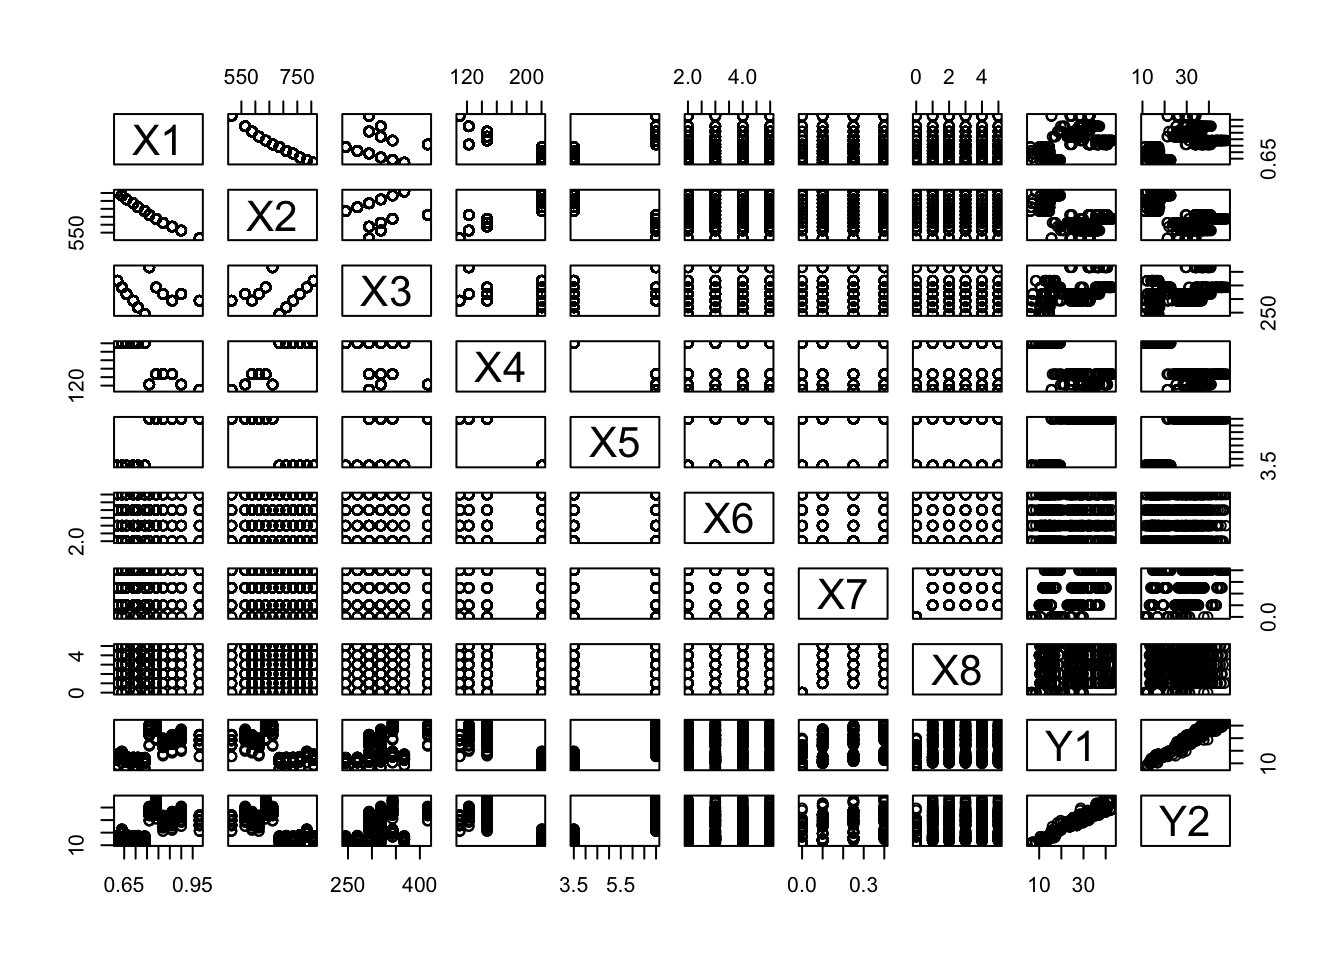
\includegraphics{_main_files/figure-latex/unnamed-chunk-129-1.pdf}

\begin{Shaded}
\begin{Highlighting}[]
\NormalTok{fit0 \textless{}{-}}\StringTok{ }\KeywordTok{lm}\NormalTok{(Y1 }\OperatorTok{\textasciitilde{}}\StringTok{ }\NormalTok{X1 }\OperatorTok{+}\StringTok{ }\NormalTok{X2 }\OperatorTok{+}\StringTok{ }\NormalTok{X3 }\OperatorTok{+}\StringTok{ }\NormalTok{X4 }\OperatorTok{+}\StringTok{ }\NormalTok{X5 }\OperatorTok{+}\StringTok{ }\NormalTok{X6 }\OperatorTok{+}\StringTok{ }\NormalTok{X7 }\OperatorTok{+}\StringTok{ }\NormalTok{X8, }\DataTypeTok{data =}\NormalTok{ energy) }\CommentTok{\# modelo saturado}
\KeywordTok{summary}\NormalTok{(fit0)}
\end{Highlighting}
\end{Shaded}

\begin{verbatim}
## 
## Call:
## lm(formula = Y1 ~ X1 + X2 + X3 + X4 + X5 + X6 + X7 + X8, data = energy)
## 
## Residuals:
##    Min     1Q Median     3Q    Max 
## -9.897 -1.320 -0.025  1.353  7.705 
## 
## Coefficients: (1 not defined because of singularities)
##              Estimate Std. Error t value Pr(>|t|)    
## (Intercept)  84.01342   19.03361    4.41  1.2e-05 ***
## X1          -64.77343   10.28945   -6.30  5.2e-10 ***
## X2           -0.08729    0.01708   -5.11  4.0e-07 ***
## X3            0.06081    0.00665    9.15  < 2e-16 ***
## X4                 NA         NA      NA       NA    
## X5            4.16995    0.33799   12.34  < 2e-16 ***
## X6           -0.02333    0.09470   -0.25   0.8055    
## X7           19.93274    0.81399   24.49  < 2e-16 ***
## X8            0.20378    0.06992    2.91   0.0037 ** 
## ---
## Signif. codes:  0 '***' 0.001 '**' 0.01 '*' 0.05 '.' 0.1 ' ' 1
## 
## Residual standard error: 2.93 on 760 degrees of freedom
## Multiple R-squared:  0.916,  Adjusted R-squared:  0.915 
## F-statistic: 1.19e+03 on 7 and 760 DF,  p-value: <2e-16
\end{verbatim}

\begin{Shaded}
\begin{Highlighting}[]
\NormalTok{fit1 \textless{}{-}}\StringTok{ }\KeywordTok{step}\NormalTok{(fit0)  }\CommentTok{\# filtrando as variáveis com stepwise}
\end{Highlighting}
\end{Shaded}

\begin{verbatim}
## Start:  AIC=1661
## Y1 ~ X1 + X2 + X3 + X4 + X5 + X6 + X7 + X8
## 
## 
## Step:  AIC=1661
## Y1 ~ X1 + X2 + X3 + X5 + X6 + X7 + X8
## 
##        Df Sum of Sq   RSS  AIC
## - X6    1         1  6544 1659
## <none>               6544 1661
## - X8    1        73  6617 1668
## - X2    1       225  6769 1685
## - X1    1       341  6885 1698
## - X3    1       721  7264 1740
## - X5    1      1311  7854 1800
## - X7    1      5163 11707 2106
## 
## Step:  AIC=1659
## Y1 ~ X1 + X2 + X3 + X5 + X7 + X8
## 
##        Df Sum of Sq   RSS  AIC
## <none>               6544 1659
## - X8    1        73  6617 1666
## - X2    1       225  6769 1683
## - X1    1       341  6886 1697
## - X3    1       721  7265 1738
## - X5    1      1311  7855 1798
## - X7    1      5163 11707 2104
\end{verbatim}

\begin{Shaded}
\begin{Highlighting}[]
\KeywordTok{summary}\NormalTok{(fit1)}
\end{Highlighting}
\end{Shaded}

\begin{verbatim}
## 
## Call:
## lm(formula = Y1 ~ X1 + X2 + X3 + X5 + X7 + X8, data = energy)
## 
## Residuals:
##    Min     1Q Median     3Q    Max 
## -9.931 -1.319 -0.026  1.359  7.717 
## 
## Coefficients:
##              Estimate Std. Error t value Pr(>|t|)    
## (Intercept)  83.93176   19.01898    4.41  1.2e-05 ***
## X1          -64.77343   10.28310   -6.30  5.1e-10 ***
## X2           -0.08729    0.01706   -5.12  4.0e-07 ***
## X3            0.06081    0.00664    9.15  < 2e-16 ***
## X5            4.16995    0.33778   12.35  < 2e-16 ***
## X7           19.93274    0.81348   24.50  < 2e-16 ***
## X8            0.20378    0.06987    2.92   0.0036 ** 
## ---
## Signif. codes:  0 '***' 0.001 '**' 0.01 '*' 0.05 '.' 0.1 ' ' 1
## 
## Residual standard error: 2.93 on 761 degrees of freedom
## Multiple R-squared:  0.916,  Adjusted R-squared:  0.916 
## F-statistic: 1.39e+03 on 6 and 761 DF,  p-value: <2e-16
\end{verbatim}

Após o primeiro ajuste atribuído a \texttt{fit0} é possível notar que o coeficiente da variável \texttt{X4} não é possível de ser calculado devido a singularidades, i.e, impossibilidade de inversão das matrizes do modelo. Sendo assim, ao modelo saturado (contendo todas as variáveis candidatas) aplicou-se o método de \emph{stepwise}, proposto por (Efroymson \protect\hyperlink{ref-efroymson1960multiple}{1960}) e utilizado para selecionar variáveis. Este método busca automaticamente o melhor conjunto de variáveis de maneira a minimizar alguma medida, usualmente o \emph{Critério de Informação de Akaike} (AIC, na sigla em inglês), sugerido por (Akaike \protect\hyperlink{ref-akaike1974new}{1974}). De acordo com a métrica do stepwise, quanto menor o valor de AIC, melhor a combinação das variáveis.

Pelos resultados obtidos pode-se verificar que o modelo ajustado em \texttt{fit1} possui todas as variávies significativas para um \(\alpha\) inferior a 0.01, estatística F de 1387 para 6 e 761 graus de liberdade, levando a um p-value geral do modelo menor que \(2.2 \times 10^{-16}\), o que indica boa aderência aos dados. O valor do \texttt{Multiple\ R-squared} é de 0.9162, indicando que o modelo explica em torno de 92\% da variação de \texttt{Y1}. Desta forma este é um modelo aceitável, que possui coeficientes de \texttt{X1} e \texttt{X2} negativos, indicando que um aumento destas variáveis (respectivamente compactação relativa e superfície) deve reduzir a carga de aquecimento. Mais especificamente, um aumento de uma unidade na compactação relativa (\texttt{X1}) gera uma redução esperada de 64.77 unidades na carga de aquecimento, mantidas constantes as demais variáveis. As variáveis \texttt{X3}, \texttt{X5}, \texttt{X7} e \texttt{X8} possuem coeficientes positivos, levando a um impacto esperado positivo em \texttt{Y1}. Como exemplo, para cada aumento de uma unidade na altura total (\texttt{X5}) espera-se um aumento aproximando de 4.17 unidades na carga de aquecimento. As outras variáveis possuem interpretação análoga, devendo-se sempre observar o sinal dos coeficientes.

\begin{exercise}
\protect\hypertarget{exr:unnamed-chunk-130}{}{\label{exr:unnamed-chunk-130} }Refaça o Exemplo 5.2 utilizando a variável \texttt{Y2} como resposta, ajustando o modelo saturado, filtrando as variáveis com a função \texttt{step} e interpretando os resultados.
\end{exercise}

\hypertarget{regressuxe3o-loguxedstica}{%
\section{Regressão Logística}\label{regressuxe3o-loguxedstica}}

\hypertarget{variuxe1veis-binuxe1riasdicotuxf4micas}{%
\subsection{Variáveis binárias/dicotômicas}\label{variuxe1veis-binuxe1riasdicotuxf4micas}}

Em problemas aplicados é comum fazer uso de variáveis aleatórias que admitam apenas dois valores, chamadas v.a. \emph{binárias} ou \emph{dicotômicas}. Empresas de serviços financeiros podem estar interessados em clientes adimplentes/inadimpletes, hospitais em pacientes com/sem melhora, cientistas da computação em servidores operantes/inoperantes, etc. Começamos com um exemplo numérico para ilustrar.

\begin{example}
\protect\hypertarget{exm:unnamed-chunk-131}{}{\label{exm:unnamed-chunk-131} }Um banco está interessado na variável aleatória \(Y\): cliente inadimplente. Ela assume valor 1 se o cliente é inadimplente (sucesso) e 0 caso contrário (fracasso). Note que a terminologia sucesso/fracasso indica se a variável \(Y\) foi observada (1) ou não (0), ainda que `sucesso' possa não significar algo agradável.\\
Se considerarmos 40 clientes, 20 inadimplentes e 20 adimplentes, pode-se calcular a probabilidade (incondicional) de observar um ciente inadimplente (sucesso) por \(Pr(Y=1)=\frac{20}{40}=0.5\). Da mesma forma, a probabilidade (incondicional) de observar um ciente adimplente (fracasso) é dada por \(Pr(Y=0)=\frac{20}{40}=0.5\). Utilizando a linguagem R pode-se gerar a sequência de zeros e uns descrita acima, bem como as respectivas probabilidades.
\end{example}

\begin{Shaded}
\begin{Highlighting}[]
\NormalTok{n \textless{}{-}}\StringTok{ }\DecValTok{20}
\NormalTok{(y \textless{}{-}}\StringTok{ }\KeywordTok{c}\NormalTok{(}\KeywordTok{rep}\NormalTok{(}\DecValTok{0}\NormalTok{,n), }\KeywordTok{rep}\NormalTok{(}\DecValTok{1}\NormalTok{,n)))}
\end{Highlighting}
\end{Shaded}

\begin{verbatim}
##  [1] 0 0 0 0 0 0 0 0 0 0 0 0 0 0 0 0 0 0 0 0 1 1 1 1 1 1 1 1 1 1 1 1 1 1 1 1 1 1 1 1
\end{verbatim}

\begin{Shaded}
\begin{Highlighting}[]
\NormalTok{(taby \textless{}{-}}\StringTok{ }\KeywordTok{table}\NormalTok{(y))}
\end{Highlighting}
\end{Shaded}

\begin{verbatim}
## y
##  0  1 
## 20 20
\end{verbatim}

\begin{Shaded}
\begin{Highlighting}[]
\KeywordTok{prop.table}\NormalTok{(taby)}
\end{Highlighting}
\end{Shaded}

\begin{verbatim}
## y
##   0   1 
## 0.5 0.5
\end{verbatim}

Vendo a questão desta maneira pode-se considerar que a probablidade de um cliente ser inadimplente é de 50\%. É possível, porém, considerar outras variáveis para refinar esta probabilidade. Suponha uma variável \(X_1\), que ocorre em aproximadamente 20\% dos clientes adimplentes (\(Y=0\)) e em aproximadamente 90\% dos clientes inadimplentes (\(Y=1\)). Assim, visto que presença da variável \(X_1\) é maior entre os inadimplentes, intuitivamente devemos atribuir uma probabilidade maior de inadimplência a clientes que apresentem a característica \(X_1\), e menor para aquele onde a característica \(X_1\) é ausente. Novamente podemos fazer uso da linguagem R para gerar sequências similares àquelas consideradas na teoria.

\begin{Shaded}
\begin{Highlighting}[]
\KeywordTok{suppressMessages}\NormalTok{(}\KeywordTok{library}\NormalTok{(tidyverse))}
\KeywordTok{set.seed}\NormalTok{(}\DecValTok{1}\NormalTok{); (x1 \textless{}{-}}\StringTok{ }\KeywordTok{c}\NormalTok{(}\KeywordTok{rbinom}\NormalTok{(n,}\DecValTok{1}\NormalTok{,.}\DecValTok{2}\NormalTok{), }\KeywordTok{rbinom}\NormalTok{(n,}\DecValTok{1}\NormalTok{,.}\DecValTok{9}\NormalTok{)))  }\CommentTok{\# gerando sequência pseudoaleatória}
\end{Highlighting}
\end{Shaded}

\begin{verbatim}
##  [1] 0 0 0 1 0 1 1 0 0 0 0 0 0 0 0 0 0 1 0 0 0 1 1 1 1 1 1 1 1 1 1 1 1 1 1 1 1 1 1 1
\end{verbatim}

Note na saída abaixo que o segmento indicado por \(\texttt{\$}\)`\(\texttt{0}\)` refere-se ao grupo onde \(X_1=0\), e \(\texttt{\$}\)`\(\texttt{1}\)` onde \(X_1=1\).

\begin{Shaded}
\begin{Highlighting}[]
\KeywordTok{by}\NormalTok{(y,x1,table) }\OperatorTok{\%\textgreater{}\%}\StringTok{   }\CommentTok{\# contando o número de zeros e uns em y separado por x1}
\StringTok{  }\KeywordTok{lapply}\NormalTok{(prop.table) }\CommentTok{\# calculando as proporções }
\end{Highlighting}
\end{Shaded}

\begin{verbatim}
## $`0`
## 
##      0      1 
## 0.9412 0.0588 
## 
## $`1`
## 
##     0     1 
## 0.174 0.826
\end{verbatim}

Note que a probabilidade de inadimplência no grupo onde \(X_1\) não é observada é igual a \(Pr(Y=1|X_1=0) = 0.05882353\). No grupo de clientes que apresentam a característica \(X_1\) esta probabilidade sobe para \(Pr(Y=1|X_1=1) = 0.826087\).

Finalmente é considerada uma variável \(X_2\), que aparece em aproximadamente metade dos clientes inadimplentes e em aproximadamente metade dos adimplentes. Assim, observar a característica \(X_2\) não deve trazer informação sobre a probabilidade de inadimplência, simbolizada pela probabilidade condicional \(Pr(Y=1|X_2 = x_2)\), \(x_2 \in \{0,1\}\).

\begin{Shaded}
\begin{Highlighting}[]
\KeywordTok{set.seed}\NormalTok{(}\DecValTok{1}\NormalTok{); (x2 \textless{}{-}}\StringTok{ }\KeywordTok{rbinom}\NormalTok{(}\DecValTok{2}\OperatorTok{*}\NormalTok{n,}\DecValTok{1}\NormalTok{,.}\DecValTok{5}\NormalTok{)) }\CommentTok{\# simulando valores de X2}
\end{Highlighting}
\end{Shaded}

\begin{verbatim}
##  [1] 0 0 1 1 0 1 1 1 1 0 0 0 1 0 1 0 1 1 0 1 1 0 1 0 0 0 0 0 1 0 0 1 0 0 1 1 1 0 1 0
\end{verbatim}

\begin{Shaded}
\begin{Highlighting}[]
\KeywordTok{by}\NormalTok{(y,x2,table) }\OperatorTok{\%\textgreater{}\%}\StringTok{  }\CommentTok{\# contando os zeros e uns de y, separados pelos valores de X2}
\StringTok{  }\KeywordTok{lapply}\NormalTok{(prop.table) }\CommentTok{\# transformando a contagem em proporção}
\end{Highlighting}
\end{Shaded}

\begin{verbatim}
## $`0`
## 
##     0     1 
## 0.429 0.571 
## 
## $`1`
## 
##     0     1 
## 0.579 0.421
\end{verbatim}

\hypertarget{o-modelo-de-regressuxe3o-loguxedstica}{%
\subsection{O modelo de regressão logística}\label{o-modelo-de-regressuxe3o-loguxedstica}}

A \emph{regressão logística} pertence à classe dos \emph{modelos lineares generalizados}, descrita em detalhes por (McCullagh and Nelder \protect\hyperlink{ref-mccullagh1989generalized}{1989}), (Agresti \protect\hyperlink{ref-agresti2007introduction}{2007}) e (Paula \protect\hyperlink{ref-paula2013modelos}{2013}). Seja \(Y\) uma variável aleatória binária com distribuição binimial de probablidade de sucesso \(\pi(x)\). A notação \(\pi(x)\) sugere que a probabilidade de sucesso está condicionada a um valor/categoria \(x\). Desta forma, \(\pi(x) = Pr(Y=1|X=x)\). Define-se a função \emph{logito} conforme a Eq. @ref(eq:logit\_uni), onde \(\mathrm{log}\) indica o logaritmo na base \(e \approx 2.718281828459\).

\begin{equation}
\mathrm{logito}\left[ \pi(x) \right] = \mathrm{log} \left( \dfrac{\pi(x)}{1-\pi(x)} \right) = \beta_0 + \beta_1 x
(\#eq:logit_uni)
\end{equation}
Isolando \(\pi(x)\) na Eq. @ref(eq:logit\_uni) obtém-se

\begin{equation}
\pi(x) = \dfrac{e^{\beta_0 + \beta_1 x}}{1+e^{\beta_0 + \beta_1 x}}
(\#eq:pix_uni)
\end{equation}

\begin{example}
\protect\hypertarget{exm:unnamed-chunk-136}{}{\label{exm:unnamed-chunk-136} }Considerando novamente as informações do Exemplo 8.1, vamos agora utilizar a estrutura das Equações @ref(eq:logit\_uni) e @ref(eq:pix\_uni) para abordar o problema.
\end{example}

\begin{Shaded}
\begin{Highlighting}[]
\CommentTok{\# modelo 1}
\NormalTok{x1 \textless{}{-}}\StringTok{ }\KeywordTok{as.factor}\NormalTok{(x1)  }\CommentTok{\# convertendo em fator para usar a função glm}
\NormalTok{fit1 \textless{}{-}}\StringTok{ }\KeywordTok{glm}\NormalTok{(y }\OperatorTok{\textasciitilde{}}\StringTok{ }\NormalTok{x1, }\DataTypeTok{family =} \StringTok{\textquotesingle{}binomial\textquotesingle{}}\NormalTok{) }\CommentTok{\# ajustando modelo logístico}
\KeywordTok{summary}\NormalTok{(fit1) }\CommentTok{\# detalhamento do modelo}
\end{Highlighting}
\end{Shaded}

\begin{verbatim}
## 
## Call:
## glm(formula = y ~ x1, family = "binomial")
## 
## Deviance Residuals: 
##    Min      1Q  Median      3Q     Max  
## -1.870  -0.348   0.135   0.618   2.380  
## 
## Coefficients:
##             Estimate Std. Error z value Pr(>|z|)    
## (Intercept)    -2.77       1.03   -2.69  0.00715 ** 
## x11             4.33       1.17    3.71  0.00021 ***
## ---
## Signif. codes:  0 '***' 0.001 '**' 0.01 '*' 0.05 '.' 0.1 ' ' 1
## 
## (Dispersion parameter for binomial family taken to be 1)
## 
##     Null deviance: 55.452  on 39  degrees of freedom
## Residual deviance: 28.860  on 38  degrees of freedom
## AIC: 32.86
## 
## Number of Fisher Scoring iterations: 5
\end{verbatim}

Note que o intercepto \(\hat{\beta}_0 = -2.773\) é significativo (\(p-value = 0.00715\)), bem como o coeficiente que indica a presença do atributo \(X_1\), \(\hat{\beta}_1 = 4.331\) (\(p-value = 0.00021\)). Assim, pode-se considerar o modelo conforme Eq. @ref(eq:logit\_uni), na forma \[\mathrm{log} \left( \dfrac{\pi(x)}{1-\pi(x)} \right) = -2.773 + 4.331 I_{x_1}. \] A simbologia \(I_{x_1}\) indica uma variável \emph{indicadora} da presença do atributo \(X_1\). Assim, se a pessoa possuir o atributo \(X_1\) considera-se \(I_{x_1}=1\), e \(I_{x_1}=0\) caso contrário. Este é um modelo conhecido como \emph{casela de referência}, visto que a variável \(X_1\) é categórica. Desta forma, uma das categorias/níveis da variável é escolhida como a (casela de) referência. Por padrão, o R utiliza a primeira da ordem numérica/alfabética, no caso \(X_1=0\). Desta forma, se a pessoa não possui a característica \(X_1\), pode-se calcular sua probabilidade de inadimplência pela Eq. @ref(eq:pix\_uni), dada por \[Pr(Y=1|X_1=0) = \pi(0) = \dfrac{e^{-2.773 + 4.331 \times 0}}{1+e^{-2.773 + 4.331 \times 0}} \approx 0.05882353.\] No caso de alguém que possui a característica \(X_1\), \[Pr(Y=1|X_1=1) = \pi(1) = \dfrac{e^{-2.773 + 4.331 \times 1}}{1+e^{-2.773 + 4.331 \times 1}} \approx 0.826087.\]

\begin{Shaded}
\begin{Highlighting}[]
\CommentTok{\# modelo 1}
\KeywordTok{exp}\NormalTok{(}\KeywordTok{coef}\NormalTok{(fit1)[}\DecValTok{1}\NormalTok{])}\OperatorTok{/}\NormalTok{(}\DecValTok{1}\OperatorTok{+}\KeywordTok{exp}\NormalTok{(}\KeywordTok{coef}\NormalTok{(fit1)[}\DecValTok{1}\NormalTok{])) }\CommentTok{\# Pr(Y = 1 | X1 = 0)}
\end{Highlighting}
\end{Shaded}

\begin{verbatim}
## (Intercept) 
##      0.0588
\end{verbatim}

\begin{Shaded}
\begin{Highlighting}[]
\KeywordTok{exp}\NormalTok{(}\KeywordTok{sum}\NormalTok{(}\KeywordTok{coef}\NormalTok{(fit1)))}\OperatorTok{/}\NormalTok{(}\DecValTok{1}\OperatorTok{+}\KeywordTok{exp}\NormalTok{(}\KeywordTok{sum}\NormalTok{(}\KeywordTok{coef}\NormalTok{(fit1)))) }\CommentTok{\# Pr(Y = 1 | X1 = 1)}
\end{Highlighting}
\end{Shaded}

\begin{verbatim}
## [1] 0.826
\end{verbatim}

O mesmo procedimento considerado para \(X_1\) pode ser realizado para \(X_2\). Note que o intercepto \(\hat{\beta}_0 = 0.2877\) é \textbf{não} significativo (\(p-value = 0.514\)), bem como o coeficiente que indica a presença do atributo \(X_2\), \(\hat{\beta}_1 = -0.6061\) (\(p-value = 0.344\)).

\begin{Shaded}
\begin{Highlighting}[]
\CommentTok{\# modelo 2}
\NormalTok{x2 \textless{}{-}}\StringTok{ }\KeywordTok{as.factor}\NormalTok{(x2)  }\CommentTok{\# convertendo em fator para usar a função glm}
\NormalTok{fit2 \textless{}{-}}\StringTok{ }\KeywordTok{glm}\NormalTok{(y }\OperatorTok{\textasciitilde{}}\StringTok{ }\NormalTok{x2, }\DataTypeTok{family =} \StringTok{\textquotesingle{}binomial\textquotesingle{}}\NormalTok{) }\CommentTok{\# ajustando modelo logístico}
\KeywordTok{summary}\NormalTok{(fit2) }\CommentTok{\# detalhamento do modelo}
\end{Highlighting}
\end{Shaded}

\begin{verbatim}
## 
## Call:
## glm(formula = y ~ x2, family = "binomial")
## 
## Deviance Residuals: 
##     Min       1Q   Median       3Q      Max  
## -1.3018  -1.0455   0.0062   1.0579   1.3153  
## 
## Coefficients:
##             Estimate Std. Error z value Pr(>|z|)
## (Intercept)    0.288      0.441    0.65     0.51
## x21           -0.606      0.641   -0.95     0.34
## 
## (Dispersion parameter for binomial family taken to be 1)
## 
##     Null deviance: 55.452  on 39  degrees of freedom
## Residual deviance: 54.546  on 38  degrees of freedom
## AIC: 58.55
## 
## Number of Fisher Scoring iterations: 4
\end{verbatim}

Desta maneira o modelo não deve ser utilizado, mas para efeito de comparação com os resultados do Exemplo 8.1 são calculadas as probabilidades de sucesso condicionadas a \(X_2=0\) e \(X_2=1\).

\begin{Shaded}
\begin{Highlighting}[]
\CommentTok{\# modelo 2}
\KeywordTok{exp}\NormalTok{(}\KeywordTok{coef}\NormalTok{(fit2)[}\DecValTok{1}\NormalTok{])}\OperatorTok{/}\NormalTok{(}\DecValTok{1}\OperatorTok{+}\KeywordTok{exp}\NormalTok{(}\KeywordTok{coef}\NormalTok{(fit2)[}\DecValTok{1}\NormalTok{])) }\CommentTok{\# Pr(Y = 1 | X2 = 0)}
\end{Highlighting}
\end{Shaded}

\begin{verbatim}
## (Intercept) 
##       0.571
\end{verbatim}

\begin{Shaded}
\begin{Highlighting}[]
\KeywordTok{exp}\NormalTok{(}\KeywordTok{sum}\NormalTok{(}\KeywordTok{coef}\NormalTok{(fit2)))}\OperatorTok{/}\NormalTok{(}\DecValTok{1}\OperatorTok{+}\KeywordTok{exp}\NormalTok{(}\KeywordTok{sum}\NormalTok{(}\KeywordTok{coef}\NormalTok{(fit2)))) }\CommentTok{\# Pr(Y = 1 | X2 = 1)}
\end{Highlighting}
\end{Shaded}

\begin{verbatim}
## [1] 0.421
\end{verbatim}

\begin{exercise}
\protect\hypertarget{exr:unnamed-chunk-141}{}{\label{exr:unnamed-chunk-141} }Considere o conjunto de dados apresentado por Ronny Kohavi e Barry Becker, disponível em \url{https://archive.ics.uci.edu/ml/datasets/adult}. Considere um modelo de regressão logística para avaliar as características que mais impactam no salario das pessoas (acima ou abaixo de 50 mil dólares).
\end{exercise}

\begin{Shaded}
\begin{Highlighting}[]
\CommentTok{\# lendo e arrumando os dados}
\NormalTok{dat \textless{}{-}}\StringTok{ }\KeywordTok{read.table}\NormalTok{(}\StringTok{\textquotesingle{}https://archive.ics.uci.edu/ml/machine{-}learning{-}databases/adult/adult.data\textquotesingle{}}\NormalTok{,}
                  \DataTypeTok{sep =} \StringTok{\textquotesingle{},\textquotesingle{}}\NormalTok{)}
\NormalTok{dat \textless{}{-}}\StringTok{ }\NormalTok{dat[,}\OperatorTok{{-}}\KeywordTok{c}\NormalTok{(}\DecValTok{3}\NormalTok{,}\DecValTok{9}\NormalTok{)]}
\KeywordTok{colnames}\NormalTok{(dat) \textless{}{-}}\StringTok{ }\KeywordTok{c}\NormalTok{(}\StringTok{\textquotesingle{}idade\textquotesingle{}}\NormalTok{,}\StringTok{\textquotesingle{}tipoTrabalho\textquotesingle{}}\NormalTok{,}\StringTok{\textquotesingle{}educacao\textquotesingle{}}\NormalTok{,}\StringTok{\textquotesingle{}anosEstudo\textquotesingle{}}\NormalTok{,}\StringTok{\textquotesingle{}estadoCivil\textquotesingle{}}\NormalTok{,}\StringTok{\textquotesingle{}ocupacao\textquotesingle{}}\NormalTok{,}
                   \StringTok{\textquotesingle{}relacao\textquotesingle{}}\NormalTok{,}\StringTok{\textquotesingle{}genero\textquotesingle{}}\NormalTok{,}\StringTok{\textquotesingle{}ganhoCapital\textquotesingle{}}\NormalTok{,}\StringTok{\textquotesingle{}perdaCapital\textquotesingle{}}\NormalTok{,}\StringTok{\textquotesingle{}horasPorSemana\textquotesingle{}}\NormalTok{,}
                   \StringTok{\textquotesingle{}paisOrigem\textquotesingle{}}\NormalTok{,}\StringTok{\textquotesingle{}salario\textquotesingle{}}\NormalTok{)}
\end{Highlighting}
\end{Shaded}

\hypertarget{aprendizadodemaquina}{%
\chapter{Aprendizado de Máquina}\label{aprendizadodemaquina}}

A aplicação de \emph{aprendizado de máquina} ou \emph{modelagem algorítmica} está em crescente expansão. A aplicação deste tipo de metodologia usualmente utiliza \emph{modelagem preditiva}, e não inferencial. Para maiores detalhes veja a discussão nas Seções 1.2 e 1.3 de (Izbicki and Santos \protect\hyperlink{ref-izbicki2020aprendizado}{2020}), bem como nos slides disponibilizados pelo professor \href{https://github.com/filipezabala/modelagem_preditiva}{neste} link.

\hypertarget{anuxe1lise-de-componentes-principais-pca}{%
\section{\texorpdfstring{Análise de Componentes Principais (\emph{PCA})}{Análise de Componentes Principais (PCA)}}\label{anuxe1lise-de-componentes-principais-pca}}

A \emph{Análise de Componentes Principais} (\emph{PCA}, na sigla em inglês) é uma técnica de redução de dimensionalidade usualmente aplicada a um grande número de variáveis relacionadas, de forma a capturar o máximo possível da variabilidade do conjunto de dados. Foi introduzida por (Pearson \protect\hyperlink{ref-pearson1901on}{1901}) e estudada independentemente por (Hotelling \protect\hyperlink{ref-hotelling1933analysis}{1933}) e outros pesquisadores que abordaram o problema de formas variadas. Considerando a definição de (Bishop \protect\hyperlink{ref-bishop1999bayesian}{1999}), seja um conjunto de dados \(X\) de dimensão \(n \times p\) composto por \(n\) vetores \(p\)-dimensionais conforme indicado a seguir. \[ X = \begin{bmatrix} x_{1,1} & x_{1,2} & \cdots & x_{1,p} \\ x_{2,1} & x_{2,2} & \cdots & x_{2,p} \\ \vdots & \vdots & \ddots & \vdots \\ x_{n,1} & x_{n,2} & \cdots & x_{n,p} \end{bmatrix} = \begin{bmatrix} \boldsymbol{x}_{1}  \\ \boldsymbol{x}_{2} \\ \vdots \\ \boldsymbol{x}_{n} \end{bmatrix} \]

Deste conjunto de dados calcula-se a matriz de covariâncias amostrais \(\boldsymbol{S}\) dada por
\begin{equation}
\boldsymbol{S} = \dfrac{1}{n} \sum_{i=1}^{n} (\boldsymbol{x}_{i} - \bar{\boldsymbol{x}}) (\boldsymbol{x}_{i} - \bar{\boldsymbol{x}})^T,
\label{eq:cov}
\end{equation}
onde \(\bar{\boldsymbol{x}} = n^{-1} \sum_{i=1}^{n} \boldsymbol{x}_{i}\) é o vetor de médias amostrais. São obtidos os autovetores \(\boldsymbol{u}_i\) e os autovalores \(\lambda_i\) de \(\boldsymbol{S}\) pela equação
\begin{equation}
\boldsymbol{Su}_i = \lambda_i \boldsymbol{u}_i,
\label{eq:av}
\end{equation}
\(i=1,\ldots,p\). Os autovetores correspondentes aos \(q\) maiores autovetores (\(q<p\)) são mantidos, e uma representação de dimensão reduzida é definida por uma combinação linear dos autovetores e dos dados deslocados pela média. Matematicamente, \(d_n=\boldsymbol{U}^T(\boldsymbol{x}_n - \boldsymbol{\bar{x}})^T\) onde \(\boldsymbol{U}_q=(\boldsymbol{u}_1,\ldots,\boldsymbol{u}_q)\).

\begin{Shaded}
\begin{Highlighting}[]
\NormalTok{df \textless{}{-}}\StringTok{ }\NormalTok{iris[}\OperatorTok{{-}}\DecValTok{5}\NormalTok{]      }\CommentTok{\# retirando a quinta coluna, \textquotesingle{}Species\textquotesingle{}}
\NormalTok{(m \textless{}{-}}\StringTok{ }\KeywordTok{colMeans}\NormalTok{(df)) }\CommentTok{\# vetor de médias}
\end{Highlighting}
\end{Shaded}

\begin{verbatim}
## Sepal.Length  Sepal.Width Petal.Length  Petal.Width 
##         5.84         3.06         3.76         1.20
\end{verbatim}

\begin{Shaded}
\begin{Highlighting}[]
\NormalTok{(S \textless{}{-}}\StringTok{ }\KeywordTok{cov}\NormalTok{(df))      }\CommentTok{\# matriz de covariâncias}
\end{Highlighting}
\end{Shaded}

\begin{verbatim}
##              Sepal.Length Sepal.Width Petal.Length Petal.Width
## Sepal.Length       0.6857     -0.0424         1.27       0.516
## Sepal.Width       -0.0424      0.1900        -0.33      -0.122
## Petal.Length       1.2743     -0.3297         3.12       1.296
## Petal.Width        0.5163     -0.1216         1.30       0.581
\end{verbatim}

\begin{Shaded}
\begin{Highlighting}[]
\KeywordTok{eigen}\NormalTok{(S)            }\CommentTok{\# autovalores (variâncias) e autovetores de S}
\end{Highlighting}
\end{Shaded}

\begin{verbatim}
## eigen() decomposition
## $values
## [1] 4.2282 0.2427 0.0782 0.0238
## 
## $vectors
##         [,1]    [,2]    [,3]   [,4]
## [1,]  0.3614 -0.6566 -0.5820  0.315
## [2,] -0.0845 -0.7302  0.5979 -0.320
## [3,]  0.8567  0.1734  0.0762 -0.480
## [4,]  0.3583  0.0755  0.5458  0.754
\end{verbatim}

\begin{Shaded}
\begin{Highlighting}[]
\NormalTok{(av \textless{}{-}}\StringTok{ }\KeywordTok{prcomp}\NormalTok{(df))  }\CommentTok{\# via função}
\end{Highlighting}
\end{Shaded}

\begin{verbatim}
## Standard deviations (1, .., p=4):
## [1] 2.056 0.493 0.280 0.154
## 
## Rotation (n x k) = (4 x 4):
##                  PC1     PC2     PC3    PC4
## Sepal.Length  0.3614 -0.6566  0.5820  0.315
## Sepal.Width  -0.0845 -0.7302 -0.5979 -0.320
## Petal.Length  0.8567  0.1734 -0.0762 -0.480
## Petal.Width   0.3583  0.0755 -0.5458  0.754
\end{verbatim}

É possível realizar o mesmo procedimento na matriz de correlação \(R\). Esta abordagem é recomendada para evitar que os resultados sejam afetados pela escala dos valores observados.

\begin{Shaded}
\begin{Highlighting}[]
\NormalTok{(R \textless{}{-}}\StringTok{ }\KeywordTok{cor}\NormalTok{(df))  }\CommentTok{\# matriz de correlação}
\end{Highlighting}
\end{Shaded}

\begin{verbatim}
##              Sepal.Length Sepal.Width Petal.Length Petal.Width
## Sepal.Length        1.000      -0.118        0.872       0.818
## Sepal.Width        -0.118       1.000       -0.428      -0.366
## Petal.Length        0.872      -0.428        1.000       0.963
## Petal.Width         0.818      -0.366        0.963       1.000
\end{verbatim}

\begin{Shaded}
\begin{Highlighting}[]
\KeywordTok{eigen}\NormalTok{(R)        }\CommentTok{\# autovalores e autovetores de R}
\end{Highlighting}
\end{Shaded}

\begin{verbatim}
## eigen() decomposition
## $values
## [1] 2.9185 0.9140 0.1468 0.0207
## 
## $vectors
##        [,1]    [,2]   [,3]   [,4]
## [1,]  0.521 -0.3774  0.720  0.261
## [2,] -0.269 -0.9233 -0.244 -0.124
## [3,]  0.580 -0.0245 -0.142 -0.801
## [4,]  0.565 -0.0669 -0.634  0.524
\end{verbatim}

\begin{Shaded}
\begin{Highlighting}[]
\KeywordTok{prcomp}\NormalTok{(df, }\DataTypeTok{scale =}\NormalTok{ T)  }\CommentTok{\# via função, scale = TRUE}
\end{Highlighting}
\end{Shaded}

\begin{verbatim}
## Standard deviations (1, .., p=4):
## [1] 1.708 0.956 0.383 0.144
## 
## Rotation (n x k) = (4 x 4):
##                 PC1     PC2    PC3    PC4
## Sepal.Length  0.521 -0.3774  0.720  0.261
## Sepal.Width  -0.269 -0.9233 -0.244 -0.124
## Petal.Length  0.580 -0.0245 -0.142 -0.801
## Petal.Width   0.565 -0.0669 -0.634  0.524
\end{verbatim}

A proporção da variância explicada pelo \(i\)-ésimo componente principal é dada pela Eq. \(\eqref{eq:propvar}\), e pode ser visualizada em um gráfico ordenado, usualmente chamado \emph{screeplot}.
\begin{equation}
PVE_i = \dfrac{\lambda_i}{\sum_{j=1}^{p} \lambda_j}
\label{eq:propvar}
\end{equation}

\begin{Shaded}
\begin{Highlighting}[]
\NormalTok{(vS \textless{}{-}}\StringTok{ }\KeywordTok{eigen}\NormalTok{(S)}\OperatorTok{$}\NormalTok{values) }\CommentTok{\# autovalores (variâncias) a partir de S}
\end{Highlighting}
\end{Shaded}

\begin{verbatim}
## [1] 4.2282 0.2427 0.0782 0.0238
\end{verbatim}

\begin{Shaded}
\begin{Highlighting}[]
\NormalTok{vS}\OperatorTok{/}\KeywordTok{sum}\NormalTok{(vS)  }\CommentTok{\# Equação (17)}
\end{Highlighting}
\end{Shaded}

\begin{verbatim}
## [1] 0.92462 0.05307 0.01710 0.00521
\end{verbatim}

\begin{Shaded}
\begin{Highlighting}[]
\KeywordTok{screeplot}\NormalTok{(}\KeywordTok{prcomp}\NormalTok{(df), }\DataTypeTok{type =} \StringTok{\textquotesingle{}lines\textquotesingle{}}\NormalTok{)}
\end{Highlighting}
\end{Shaded}

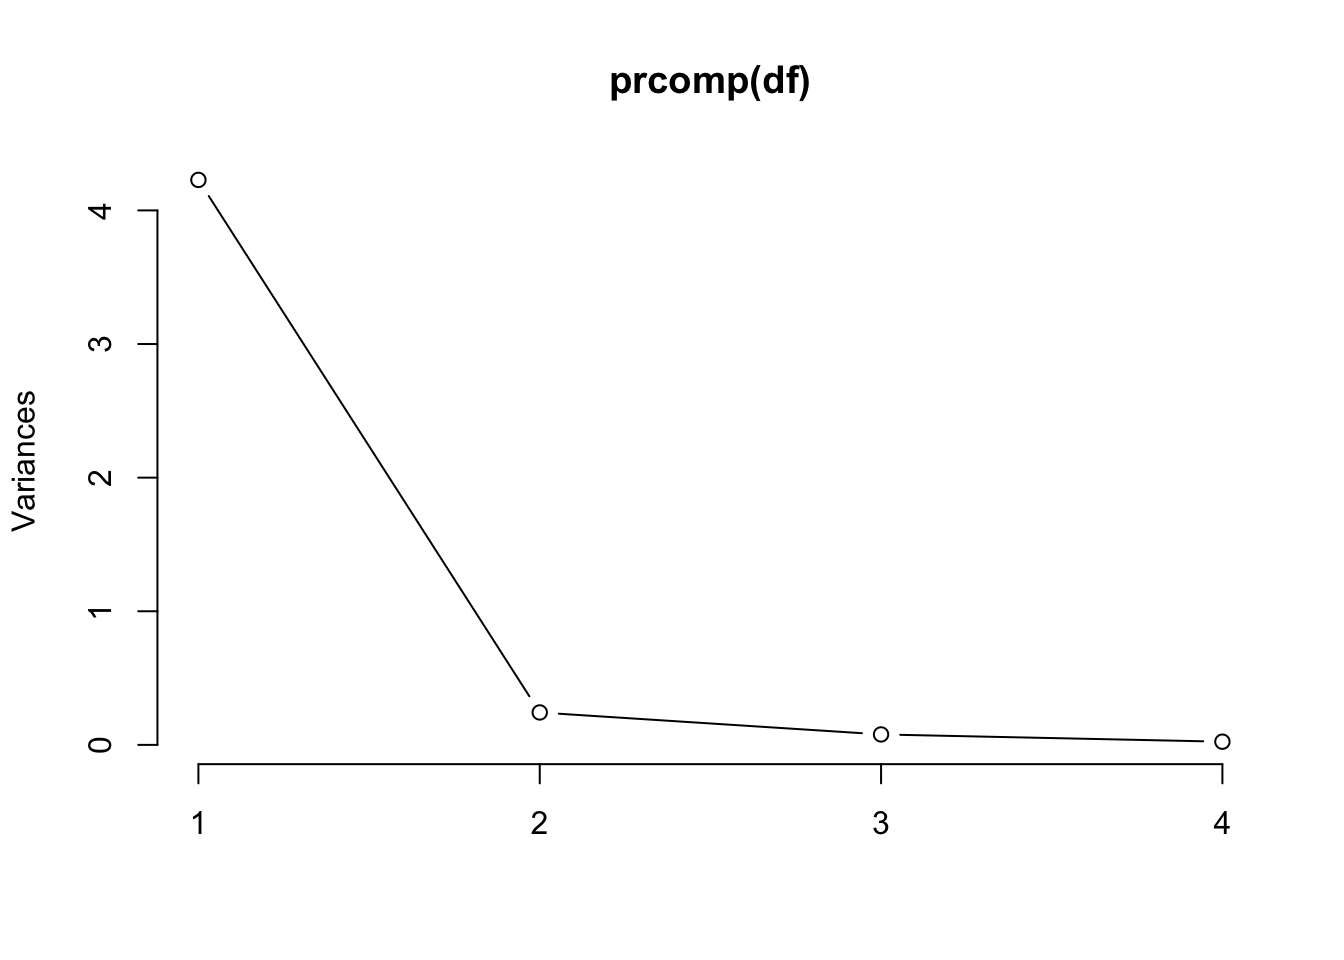
\includegraphics{_main_files/figure-latex/unnamed-chunk-145-1.pdf}

\begin{Shaded}
\begin{Highlighting}[]
\NormalTok{(vR \textless{}{-}}\StringTok{ }\KeywordTok{eigen}\NormalTok{(R)}\OperatorTok{$}\NormalTok{values) }\CommentTok{\# autovalores (variâncias) a partir de R}
\end{Highlighting}
\end{Shaded}

\begin{verbatim}
## [1] 2.9185 0.9140 0.1468 0.0207
\end{verbatim}

\begin{Shaded}
\begin{Highlighting}[]
\NormalTok{vR}\OperatorTok{/}\KeywordTok{sum}\NormalTok{(vR)  }\CommentTok{\# Equação (17)}
\end{Highlighting}
\end{Shaded}

\begin{verbatim}
## [1] 0.72962 0.22851 0.03669 0.00518
\end{verbatim}

\begin{Shaded}
\begin{Highlighting}[]
\KeywordTok{screeplot}\NormalTok{(}\KeywordTok{prcomp}\NormalTok{(df, }\DataTypeTok{scale =}\NormalTok{ T), }\DataTypeTok{type =} \StringTok{\textquotesingle{}lines\textquotesingle{}}\NormalTok{)}
\end{Highlighting}
\end{Shaded}

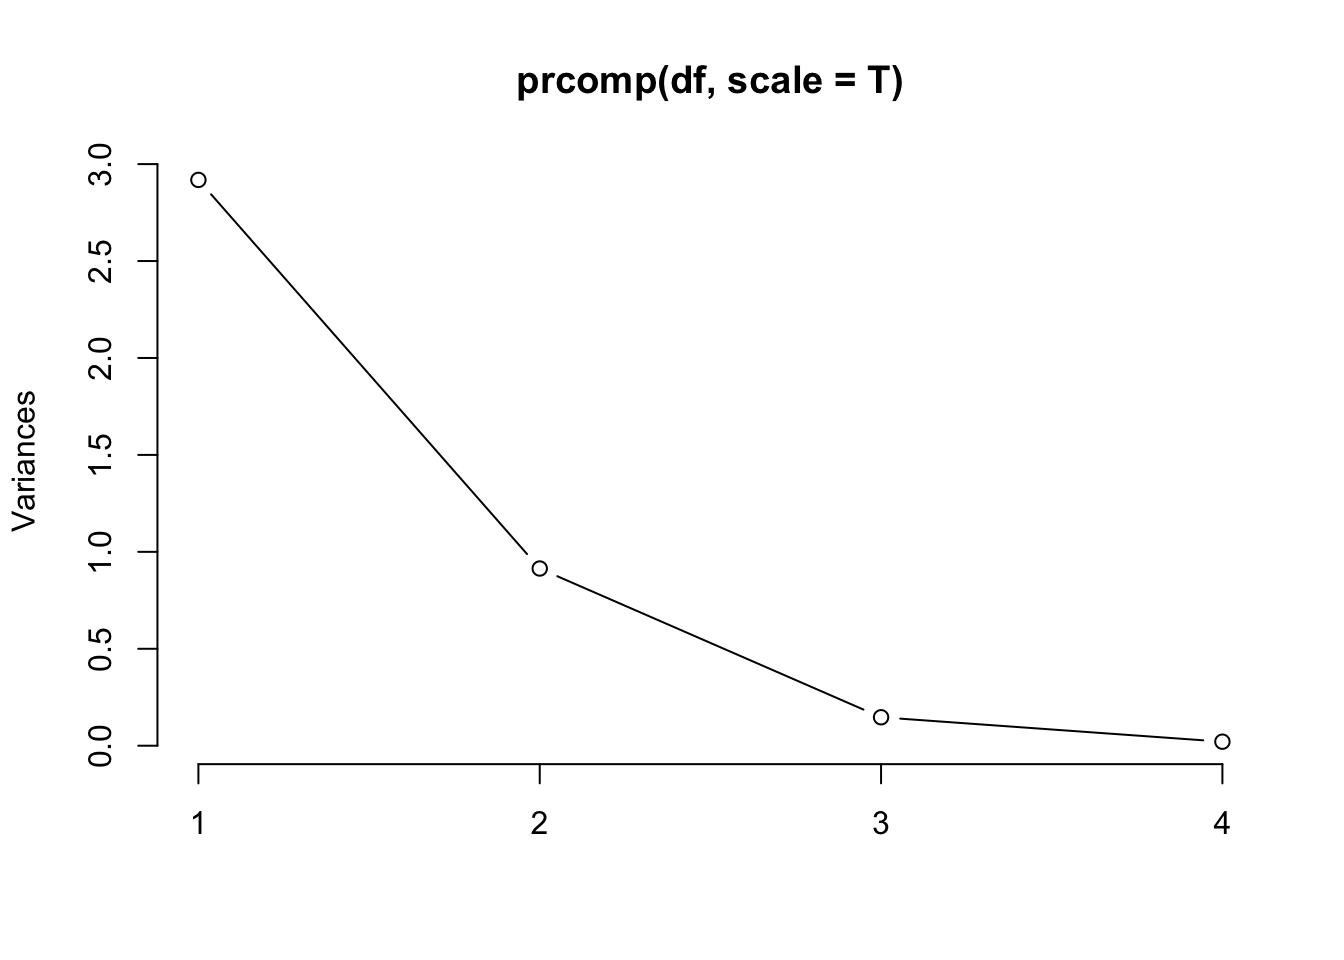
\includegraphics{_main_files/figure-latex/unnamed-chunk-145-2.pdf}

Considere o banco de dados \texttt{iris}, que contém 4 colunas numéricas com as larguras e comprimentos das pétalas e sépalas de três espécies de flores do gênero íris.

\begin{Shaded}
\begin{Highlighting}[]
\KeywordTok{head}\NormalTok{(iris)}
\end{Highlighting}
\end{Shaded}

\begin{verbatim}
##   Sepal.Length Sepal.Width Petal.Length Petal.Width Species
## 1          5.1         3.5          1.4         0.2  setosa
## 2          4.9         3.0          1.4         0.2  setosa
## 3          4.7         3.2          1.3         0.2  setosa
## 4          4.6         3.1          1.5         0.2  setosa
## 5          5.0         3.6          1.4         0.2  setosa
## 6          5.4         3.9          1.7         0.4  setosa
\end{verbatim}

Existem \({4 \choose 2} = 6\) combinações possíveis de gráficos bidimensionais, apresentados a seguir.

\begin{Shaded}
\begin{Highlighting}[]
\KeywordTok{require}\NormalTok{(gridExtra)}
\NormalTok{p1 \textless{}{-}}\StringTok{ }\KeywordTok{ggplot}\NormalTok{(iris, }\KeywordTok{aes}\NormalTok{(Sepal.Length, Sepal.Width, }\DataTypeTok{colour =}\NormalTok{ Species)) }\OperatorTok{+}\StringTok{ }\KeywordTok{geom\_point}\NormalTok{()}
\NormalTok{p2 \textless{}{-}}\StringTok{ }\KeywordTok{ggplot}\NormalTok{(iris, }\KeywordTok{aes}\NormalTok{(Sepal.Length, Petal.Length, }\DataTypeTok{colour =}\NormalTok{ Species)) }\OperatorTok{+}\StringTok{ }\KeywordTok{geom\_point}\NormalTok{()}
\NormalTok{p3 \textless{}{-}}\StringTok{ }\KeywordTok{ggplot}\NormalTok{(iris, }\KeywordTok{aes}\NormalTok{(Sepal.Length, Petal.Width, }\DataTypeTok{colour =}\NormalTok{ Species)) }\OperatorTok{+}\StringTok{ }\KeywordTok{geom\_point}\NormalTok{()}
\NormalTok{p4 \textless{}{-}}\StringTok{ }\KeywordTok{ggplot}\NormalTok{(iris, }\KeywordTok{aes}\NormalTok{(Sepal.Width, Petal.Length, }\DataTypeTok{colour =}\NormalTok{ Species)) }\OperatorTok{+}\StringTok{ }\KeywordTok{geom\_point}\NormalTok{()}
\NormalTok{p5 \textless{}{-}}\StringTok{ }\KeywordTok{ggplot}\NormalTok{(iris, }\KeywordTok{aes}\NormalTok{(Sepal.Width, Petal.Width, }\DataTypeTok{colour =}\NormalTok{ Species)) }\OperatorTok{+}\StringTok{ }\KeywordTok{geom\_point}\NormalTok{()}
\NormalTok{p6 \textless{}{-}}\StringTok{ }\KeywordTok{ggplot}\NormalTok{(iris, }\KeywordTok{aes}\NormalTok{(Petal.Length, Petal.Width, }\DataTypeTok{colour =}\NormalTok{ Species)) }\OperatorTok{+}\StringTok{ }\KeywordTok{geom\_point}\NormalTok{()}
\KeywordTok{grid.arrange}\NormalTok{(p1, p2, p3, p4, p5, p6, }\DataTypeTok{ncol =} \DecValTok{2}\NormalTok{)}
\end{Highlighting}
\end{Shaded}

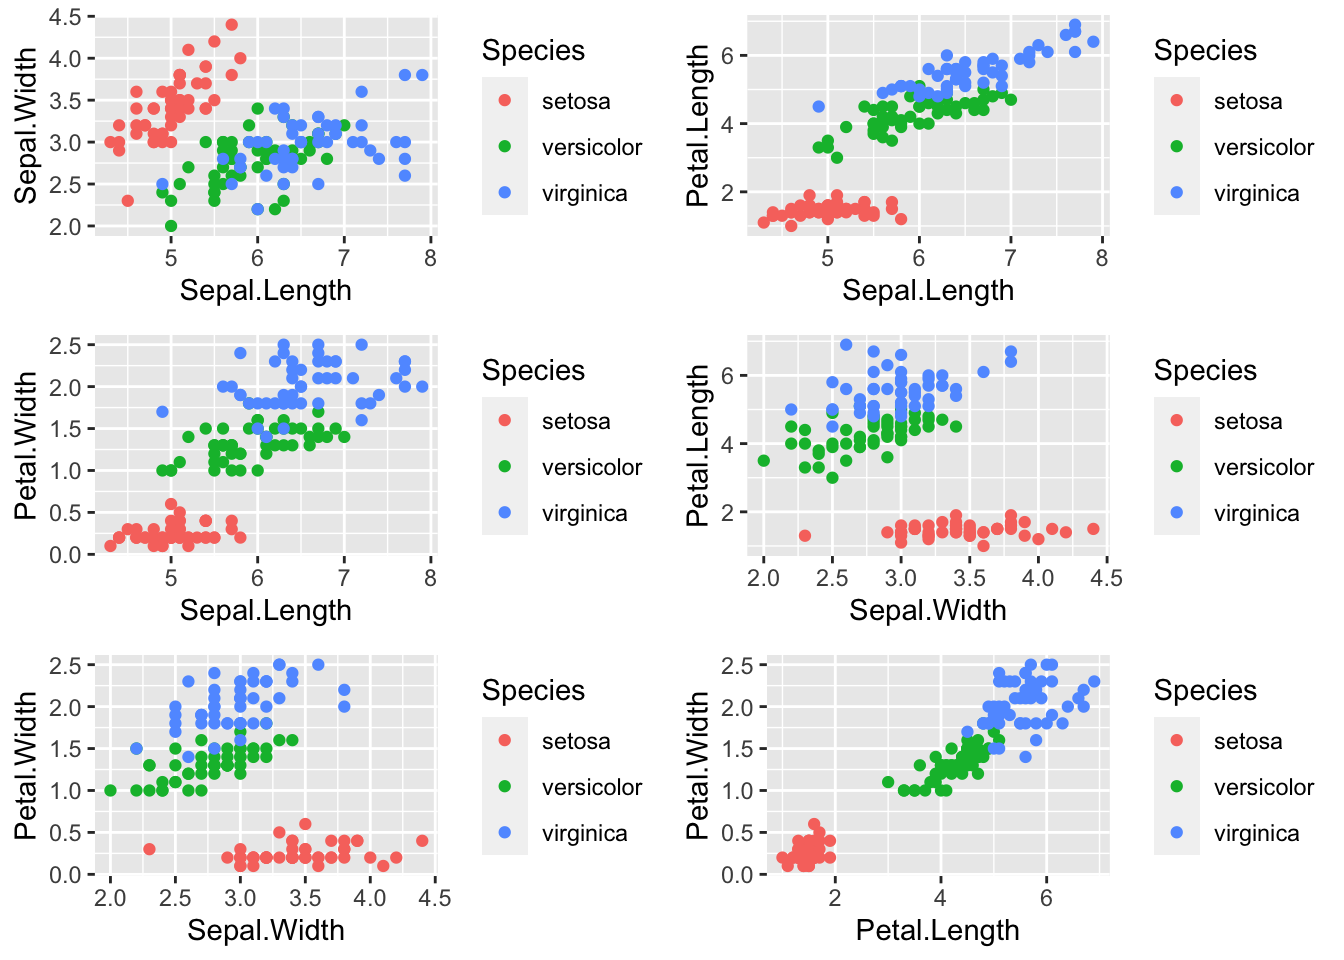
\includegraphics{_main_files/figure-latex/unnamed-chunk-147-1.pdf}

É posível utilizar o método de componentes principais para aprimorar a visualização\footnote{Exemplos baseados em \url{https://cran.r-project.org/web/packages/ggfortify/vignettes/plot_pca.html}.} da estrutura de associação entre as diferentes espécies de plantas.

\begin{Shaded}
\begin{Highlighting}[]
\KeywordTok{library}\NormalTok{(ggfortify)}
\KeywordTok{autoplot}\NormalTok{(}\KeywordTok{prcomp}\NormalTok{(df), }\DataTypeTok{data =}\NormalTok{ iris, }\DataTypeTok{colour =} \StringTok{\textquotesingle{}Species\textquotesingle{}}\NormalTok{, }\DataTypeTok{loadings =}\NormalTok{ T, }\DataTypeTok{loadings.label =}\NormalTok{ T, }\DataTypeTok{type =} \StringTok{\textquotesingle{}raw\textquotesingle{}}\NormalTok{)}
\end{Highlighting}
\end{Shaded}

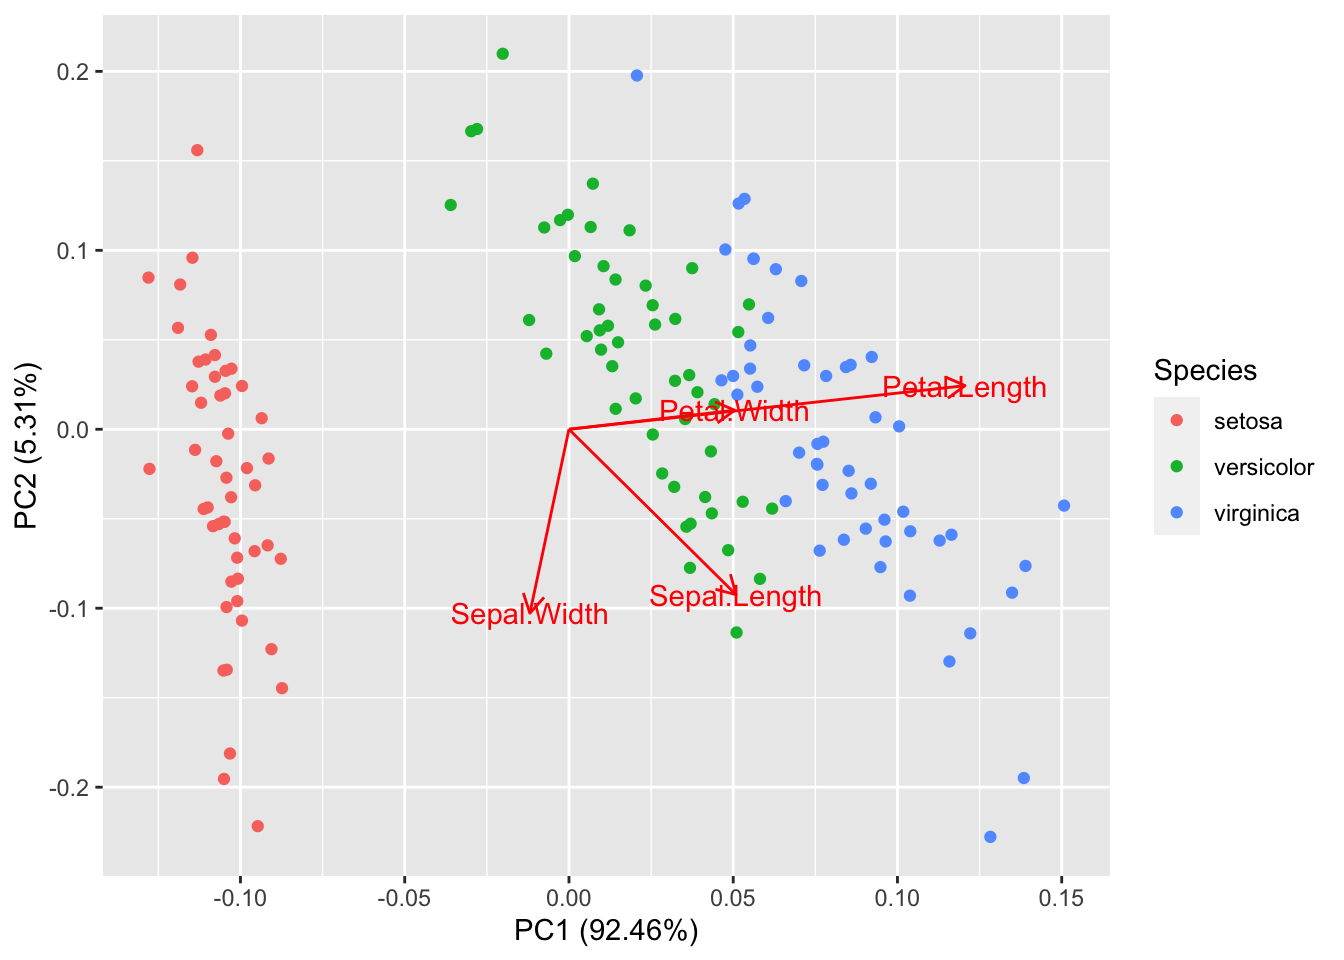
\includegraphics{_main_files/figure-latex/unnamed-chunk-148-1.pdf}

\begin{Shaded}
\begin{Highlighting}[]
\KeywordTok{autoplot}\NormalTok{(}\KeywordTok{prcomp}\NormalTok{(df, }\DataTypeTok{scale =}\NormalTok{ T), }\DataTypeTok{data =}\NormalTok{ iris, }\DataTypeTok{colour =} \StringTok{\textquotesingle{}Species\textquotesingle{}}\NormalTok{, }\DataTypeTok{loadings =}\NormalTok{ T, }\DataTypeTok{loadings.label =}\NormalTok{ T)}
\end{Highlighting}
\end{Shaded}

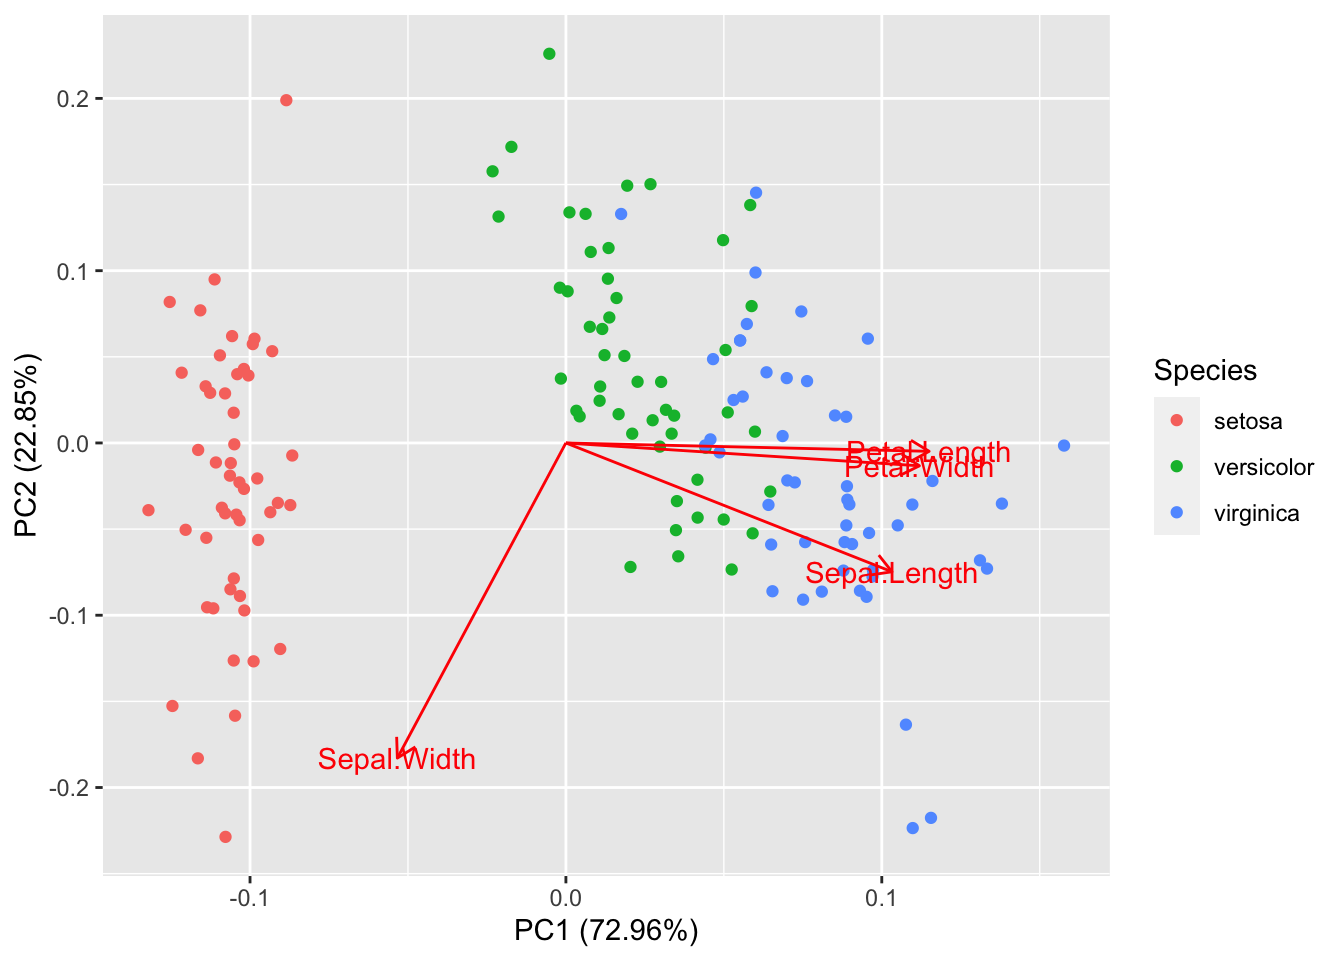
\includegraphics{_main_files/figure-latex/unnamed-chunk-148-2.pdf}

\begin{exercise}
\protect\hypertarget{exr:unnamed-chunk-149}{}{\label{exr:unnamed-chunk-149} }Considere o banco de dados sobre câncer de mama apresentado por (Dua and Graff \protect\hyperlink{ref-dua2019uci}{2019}). A partir do código abaixo, faça uma anáise de componentes principais desconsiderando as duas primeiras colunas, que indicam respectivamente o código de identificação da paciente (\texttt{V1}) e o diagnóstico (\texttt{V2}, Benigno/Maligno).\\
(a) Quais os valores de \(n\) e \(p\)?\\
(b) O que ocorre no comando \texttt{x2\ \textless{}-\ x{[},-c(1,2){]}}?\\
(c) Obtenha os autovalores e autovetores.\\
(d) Apresente o \emph{screeplot}.\\
(e) Apresente o gráfico dos dois primeiros componentes principais colorido por \texttt{V2}.\\
(f) Você considera que é possível associar os diagnósticos às variáveis \texttt{V3} a \texttt{V32}? Dica: observe se há algum tipo de agrupamento no gráfico do item (e).\\
(g) Quais variáveis mais influenciam nos compomentes principais 1 e 2? Dica: use \texttt{loadings.label\ =\ T} na função \texttt{autoplot} do item (e) e observe o gráfico.
\end{exercise}

\begin{Shaded}
\begin{Highlighting}[]
\KeywordTok{library}\NormalTok{(ggfortify)}
\NormalTok{x \textless{}{-}}\StringTok{ }\KeywordTok{read.table}\NormalTok{(}\StringTok{\textquotesingle{}https://archive.ics.uci.edu/ml/machine{-}learning{-}databases/breast{-}cancer{-}wisconsin/wdbc.data\textquotesingle{}}\NormalTok{, }\DataTypeTok{sep =} \StringTok{\textquotesingle{},\textquotesingle{}}\NormalTok{)}
\NormalTok{x2 \textless{}{-}}\StringTok{ }\NormalTok{x[,}\OperatorTok{{-}}\KeywordTok{c}\NormalTok{(}\DecValTok{1}\NormalTok{,}\DecValTok{2}\NormalTok{)]}
\end{Highlighting}
\end{Shaded}

\hypertarget{tuxe9cnicas-de-agrupamento}{%
\section{Técnicas de Agrupamento}\label{tuxe9cnicas-de-agrupamento}}

Seguindo a definição de (Hartigan \protect\hyperlink{ref-hartigan1975clustering}{1975}), \emph{agrupamento} - \emph{clustering} ou ainda \emph{segmentação de dados} - é o \emph{agrupamento de objetos similares}. Objetiva agregar observações que sejam similares em relação a características admitidas nos modelos considerados. Podem ser \emph{aglomerativas}, quando definem uma delimitação ascendente - onde cada observação inicia como um grupo e se agrega com outras ao longo das iterações - ou \emph{divisivas} se o cercamento é descendente - quando todas as observações começam em um grupo que vai sendo dividido a cada etapa.\\
A linguagem R possui diversas funções para análise de agrupamento, sendo as principais discutidas neste capítulo. Para informações atualizadas, veja \url{https://cran.r-project.org/web/views/Cluster.html}.

\hypertarget{medidas-de-similaridade-e-dissimilaridade}{%
\subsection{Medidas de similaridade e dissimilaridade}\label{medidas-de-similaridade-e-dissimilaridade}}

\emph{Distâncias} e \emph{divergências} são métricas utilizadas em problemas de classificação, agrupamento e reconhecimento de padrões. São utilizadas para medir a \emph{similaridade} ou \emph{dissimilaridade} entre pontos, vetores e distribuições. É comum realizar a \emph{padronização}, i.e., subtrair cada valor da média e dividir pelo desvio padrão da coluna à qual o valor pertence. Este procedimento pode ser realizado através da função \texttt{base::scale}.

\begin{quote}
Medida de similaridade avalia o quão similares são dois entes, ficando entre 0 (sem similariadade) e 1 (completamente similares).
\end{quote}

\begin{quote}
Medida de dissimilaridade indica o quão distintos são dois entes, ficando entre 0 (iguais) e infinito (diferentes).
\end{quote}

As seguir são apresentadas algumas das principais distâncias da literatura -- enquadradas na definição de medidas de dissimilaridade -- e calculadas entre dois vetores \(\boldsymbol{x}\) e \(\boldsymbol{y}\), usualmente linhas de uma matriz numérica. Apresenta-se ainda um pequeno banco de dados para a aplicação dos exemplos.

\begin{Shaded}
\begin{Highlighting}[]
\CommentTok{\# criando data frame \textquotesingle{}df\textquotesingle{} para os exemplos a seguir}
\NormalTok{df \textless{}{-}}\StringTok{ }\KeywordTok{data.frame}\NormalTok{(}\DataTypeTok{V1=}\KeywordTok{c}\NormalTok{(}\DecValTok{3}\NormalTok{,}\DecValTok{1}\NormalTok{), }\DataTypeTok{V2=}\KeywordTok{c}\NormalTok{(}\DecValTok{2}\NormalTok{,}\DecValTok{4}\NormalTok{))  }\CommentTok{\# vetores V1 e V2}
\KeywordTok{rownames}\NormalTok{(df) \textless{}{-}}\StringTok{ }\KeywordTok{c}\NormalTok{(}\StringTok{\textquotesingle{}x\textquotesingle{}}\NormalTok{,}\StringTok{\textquotesingle{}y\textquotesingle{}}\NormalTok{)  }\CommentTok{\# rótulo das linhas}
\NormalTok{df}
\end{Highlighting}
\end{Shaded}

\begin{verbatim}
##   V1 V2
## x  3  2
## y  1  4
\end{verbatim}

\begin{Shaded}
\begin{Highlighting}[]
\CommentTok{\# padronizando os dados}
\NormalTok{df.s \textless{}{-}}\StringTok{ }\KeywordTok{scale}\NormalTok{(df)}
\NormalTok{df.s}
\end{Highlighting}
\end{Shaded}

\begin{verbatim}
##       V1     V2
## x  0.707 -0.707
## y -0.707  0.707
## attr(,"scaled:center")
## V1 V2 
##  2  3 
## attr(,"scaled:scale")
##   V1   V2 
## 1.41 1.41
\end{verbatim}

\hypertarget{distuxe2ncia-de-manhattan}{%
\subsubsection*{Distância de Manhattan}\label{distuxe2ncia-de-manhattan}}
\addcontentsline{toc}{subsubsection}{Distância de Manhattan}

A \emph{distância de Manhattan}, \emph{norma 1} ou \(L_1\) é uma medida de dissimilaridade que avalia a distância absoluta entre dois vetores, dada pela Equação \(\eqref{eq:manh}\).
\begin{equation}
L_1 = \sum_{i=1}^{n} |x_i - y_i|
\label{eq:manh}
\end{equation}

\begin{Shaded}
\begin{Highlighting}[]
\KeywordTok{sum}\NormalTok{(}\KeywordTok{abs}\NormalTok{(df[}\DecValTok{1}\NormalTok{,]}\OperatorTok{{-}}\NormalTok{df[}\DecValTok{2}\NormalTok{,]))  }\CommentTok{\# distância manhattan aplicando Eq. (18)}
\end{Highlighting}
\end{Shaded}

\begin{verbatim}
## [1] 4
\end{verbatim}

\begin{Shaded}
\begin{Highlighting}[]
\KeywordTok{dist}\NormalTok{(df, }\DataTypeTok{method =} \StringTok{\textquotesingle{}manhattan\textquotesingle{}}\NormalTok{)  }\CommentTok{\# distância manhattan via \textquotesingle{}dist\textquotesingle{}}
\end{Highlighting}
\end{Shaded}

\begin{verbatim}
##   x
## y 4
\end{verbatim}

\begin{Shaded}
\begin{Highlighting}[]
\KeywordTok{dist}\NormalTok{(df.s, }\DataTypeTok{method =} \StringTok{\textquotesingle{}manhattan\textquotesingle{}}\NormalTok{)  }\CommentTok{\# distância manhattan via \textquotesingle{}dist\textquotesingle{} dos valores padronizados}
\end{Highlighting}
\end{Shaded}

\begin{verbatim}
##      x
## y 2.83
\end{verbatim}

\hypertarget{distuxe2ncia-euclidiana}{%
\subsubsection*{Distância euclidiana}\label{distuxe2ncia-euclidiana}}
\addcontentsline{toc}{subsubsection}{Distância euclidiana}

Uma das mais utilizadas medidas de dissimilaridade da literatura, a \emph{distância euclidiana}, \emph{norma 2} ou \(L_2\) é dada pela Equação \(\eqref{eq:eucl}\).
\begin{equation}
L_2 = \sqrt{\sum_{i=1}^{n} (x_i - y_i)^2}
\label{eq:eucl}
\end{equation}

\begin{Shaded}
\begin{Highlighting}[]
\KeywordTok{sqrt}\NormalTok{(}\KeywordTok{sum}\NormalTok{((df[}\DecValTok{1}\NormalTok{,]}\OperatorTok{{-}}\NormalTok{df[}\DecValTok{2}\NormalTok{,])}\OperatorTok{\^{}}\DecValTok{2}\NormalTok{))  }\CommentTok{\# distância euclidiana aplicando Eq. (19)}
\end{Highlighting}
\end{Shaded}

\begin{verbatim}
## [1] 2.83
\end{verbatim}

\begin{Shaded}
\begin{Highlighting}[]
\KeywordTok{dist}\NormalTok{(df, }\DataTypeTok{method =} \StringTok{\textquotesingle{}euclidean\textquotesingle{}}\NormalTok{)  }\CommentTok{\# distância euclidiana via \textquotesingle{}dist\textquotesingle{}}
\end{Highlighting}
\end{Shaded}

\begin{verbatim}
##      x
## y 2.83
\end{verbatim}

\begin{Shaded}
\begin{Highlighting}[]
\KeywordTok{dist}\NormalTok{(df.s, }\DataTypeTok{method =} \StringTok{\textquotesingle{}euclidean\textquotesingle{}}\NormalTok{)  }\CommentTok{\# distância euclidiana via \textquotesingle{}dist\textquotesingle{} dos valores padronizados}
\end{Highlighting}
\end{Shaded}

\begin{verbatim}
##   x
## y 2
\end{verbatim}

\hypertarget{distuxe2ncia-de-minkowski}{%
\subsubsection*{Distância de Minkowski}\label{distuxe2ncia-de-minkowski}}
\addcontentsline{toc}{subsubsection}{Distância de Minkowski}

A \emph{distância de Minkowski}, \emph{norma p} ou \(L_p\) é uma medida de dissimilaridade que generaliza as distâncias de Manhattan e euclidiana. É dada pela Equação \(\eqref{eq:mink}\).
\begin{equation}
L_p = \sqrt[\leftroot{-2}\uproot{3}p]{\sum_{i=1}^{n} (|x_i - y_i|)^p}
\label{eq:mink}
\end{equation}

\begin{Shaded}
\begin{Highlighting}[]
\KeywordTok{sum}\NormalTok{((}\KeywordTok{abs}\NormalTok{(df[}\DecValTok{1}\NormalTok{,]}\OperatorTok{{-}}\NormalTok{df[}\DecValTok{2}\NormalTok{,]))}\OperatorTok{\^{}}\DecValTok{5}\NormalTok{)}\OperatorTok{\^{}}\NormalTok{(}\DecValTok{1}\OperatorTok{/}\DecValTok{5}\NormalTok{)     }\CommentTok{\# distância de Minkowski com p=5 aplicando Eq. (20)}
\end{Highlighting}
\end{Shaded}

\begin{verbatim}
## [1] 2.3
\end{verbatim}

\begin{Shaded}
\begin{Highlighting}[]
\KeywordTok{dist}\NormalTok{(df, }\DataTypeTok{method =} \StringTok{\textquotesingle{}minkowski\textquotesingle{}}\NormalTok{, }\DataTypeTok{p =} \DecValTok{5}\NormalTok{) }\CommentTok{\# distância de Minkowski com p=5 via \textquotesingle{}dist\textquotesingle{}}
\end{Highlighting}
\end{Shaded}

\begin{verbatim}
##     x
## y 2.3
\end{verbatim}

\begin{Shaded}
\begin{Highlighting}[]
\KeywordTok{dist}\NormalTok{(df.s, }\DataTypeTok{method =} \StringTok{\textquotesingle{}minkowski\textquotesingle{}}\NormalTok{, }\DataTypeTok{p =} \DecValTok{5}\NormalTok{) }\CommentTok{\# dist. de Minkowski com p=5 via \textquotesingle{}dist\textquotesingle{} dos valores padronizados}
\end{Highlighting}
\end{Shaded}

\begin{verbatim}
##      x
## y 1.62
\end{verbatim}

\begin{exercise}
\protect\hypertarget{exr:unnamed-chunk-155}{}{\label{exr:unnamed-chunk-155} }Considere a função \texttt{stats::dist}.\\
(a) Verifique sua documentação, fazendo \texttt{?dist}.\\
(b) Compare as distâncias euclidiana e de Minkowski com \(p=2\). O que você observa?\\
(c) Compare as distâncias de Manhattan e de Minkowski com \(p=1\). O que você observa?
\end{exercise}

\begin{exercise}
\protect\hypertarget{exr:unnamed-chunk-156}{}{\label{exr:unnamed-chunk-156} }Considere as distâncias da Seção 7.1 aplicada às colunas numéricas do banco de dados \texttt{pib}, obtido pelo código abaixo.\\
(a) Padronize os dados e atribua a uma variável chamada \texttt{pib.s}.\\
(b) Realize os cálculos `a mão' como nos exemplos, tanto para \texttt{pib} quanto para \texttt{pib.s}.\\
(c) Realize novamente os cálculos do item (b) utilizando a função \texttt{dist}.
\end{exercise}

\begin{Shaded}
\begin{Highlighting}[]
\NormalTok{pib \textless{}{-}}\StringTok{ }\KeywordTok{read.table}\NormalTok{(}\StringTok{\textquotesingle{}http://www.filipezabala.com/data/pib.txt\textquotesingle{}}\NormalTok{, }\DataTypeTok{head =}\NormalTok{ T, }\DataTypeTok{sep =} \StringTok{\textquotesingle{}}\CharTok{\textbackslash{}t}\StringTok{\textquotesingle{}}\NormalTok{)}
\end{Highlighting}
\end{Shaded}

\hypertarget{muxe9todos-hieruxe1rquicos}{%
\section{Métodos hierárquicos}\label{muxe9todos-hieruxe1rquicos}}

Como o nome sugere, os \emph{métodos hierárquicos} buscam uma estrutura hierárquica dos grupos. Esta estrutura geralmente se dá em forma de árvore, onde os objetos são apresentados individualmente como um grupo unitário (folha/\emph{leaf}) que se aglomeram por similaridade em grupos maiores (nós/\emph{nodes}) ligados por um grande grupo que une todos elementos (raiz/\emph{root}). Os passos para realizar um agrupamento hierárquico aglomerativo estão descritos a seguir.

\textbf{ALGORITMO DE AGRUPAMENTO HIERÁRQUICO AGLOMERATIVO}

\begin{quote}
\textbf{PASSO 1} Padronizar os dados, geralmente com o uso da função \texttt{scale}.
\end{quote}

\begin{quote}
\textbf{PASSO 2} Calcular a (dis)similaridade entre cada par de objetos no conjunto de dados.
\end{quote}

\begin{quote}
\textbf{PASSO 3} Usar a função de ligação para agrupar os objetos na árvore a partir das informações de distância obtidas na passo 1.
\end{quote}

\begin{quote}
\textbf{PASSO 4} Apresentar o gráfico da árvore hierárquica em grupos (dendograma), criando uma partição dos dados.
\end{quote}

\begin{Shaded}
\begin{Highlighting}[]
\CommentTok{\# 1. padronizando os dados}
\NormalTok{USArrest.scale \textless{}{-}}\StringTok{ }\KeywordTok{scale}\NormalTok{(USArrests)}
\CommentTok{\# 2. calculando distâncias (utilizando o padrão: euclidean)}
\NormalTok{dUSA \textless{}{-}}\StringTok{ }\KeywordTok{dist}\NormalTok{(USArrest.scale)}
\CommentTok{\# 3. aplicando a função de ligação (utilizando o padrão: complete)}
\NormalTok{hc \textless{}{-}}\StringTok{ }\KeywordTok{hclust}\NormalTok{(dUSA)}
\CommentTok{\# 4. apresentando o gráfico}
\KeywordTok{plot}\NormalTok{(hc)}
\end{Highlighting}
\end{Shaded}

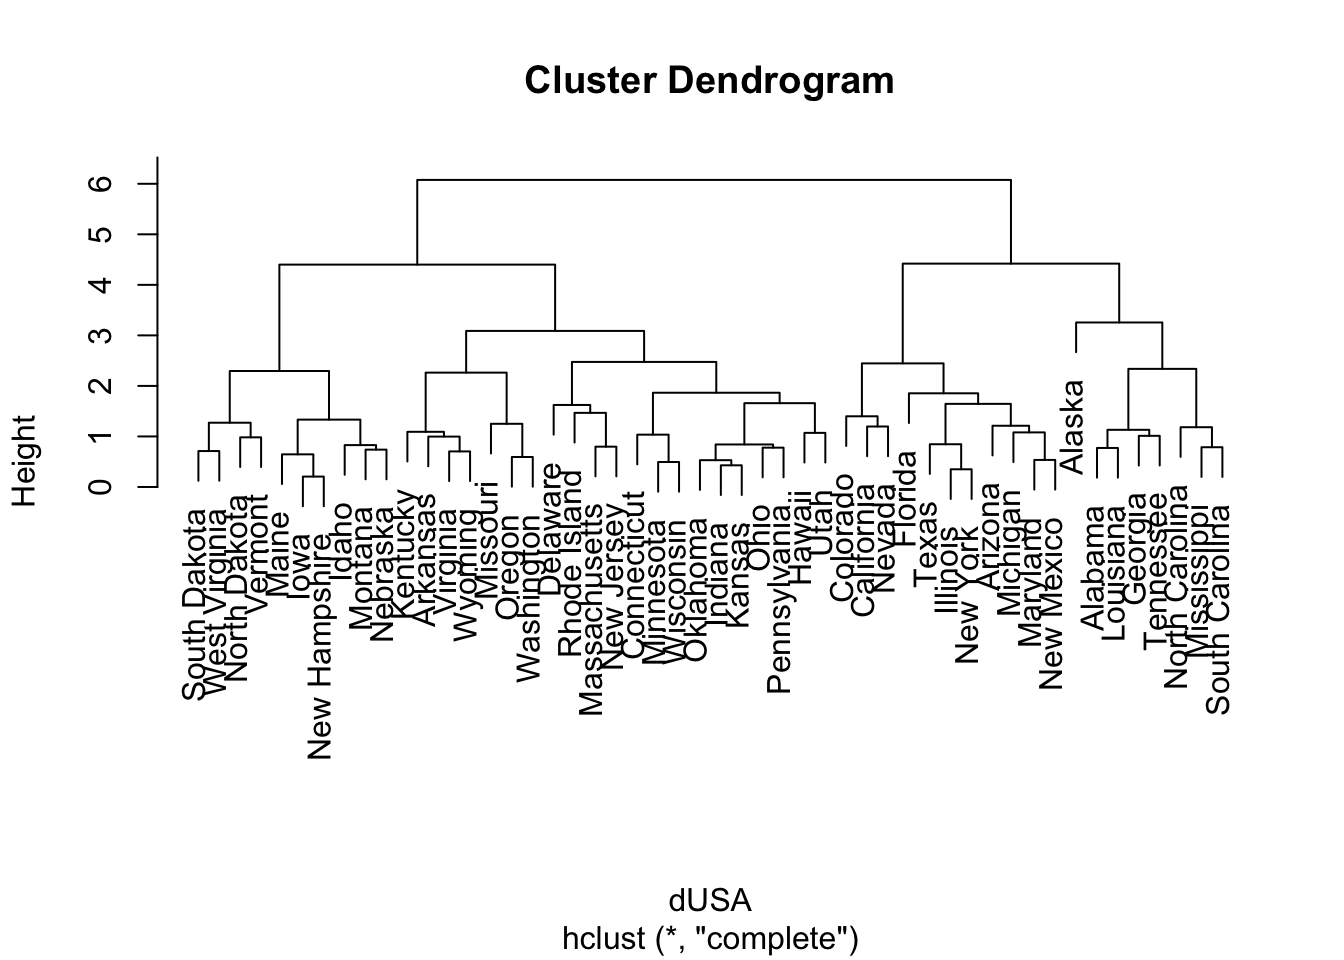
\includegraphics{_main_files/figure-latex/unnamed-chunk-158-1.pdf}

Os valores no eixo \(y\), intitulados \emph{height}, são as chamadas \emph{distâncias cofenéticas} propostas por (Sokal and Rohlf \protect\hyperlink{ref-sokal1962comparison}{1962}). O nome vem da área da Biologia chamada \href{https://pt.wikipedia.org/wiki/Fen\%C3\%A9tica}{fenética}, que estuda métodos de classificação por similaridade fenotípica. Seu cálculo não é complexo, mas pode ser trabalhoso; assim, será considerada a função \texttt{cophenetic} para a obtenção de tais distâncias. Quanto maior for seu valor, mais dissimilar são os elementos comparados. Correlação elevada entre as distâncias calculadas e as distâncias cofenéticas sugere um bom agrupamento.

\begin{Shaded}
\begin{Highlighting}[]
\CommentTok{\# Calcula a matriz de distâncias cofenéticas}
\NormalTok{coph \textless{}{-}}\StringTok{ }\KeywordTok{cophenetic}\NormalTok{(hc)}
\KeywordTok{sort}\NormalTok{(}\KeywordTok{unique}\NormalTok{(coph))}
\end{Highlighting}
\end{Shaded}

\begin{verbatim}
##  [1] 0.206 0.350 0.429 0.494 0.530 0.535 0.594 0.646 0.704 0.711 0.739 0.772 0.778 0.787 0.798 0.829 0.841 0.846 0.982 0.997
## [21] 1.012 1.035 1.071 1.080 1.092 1.131 1.183 1.197 1.212 1.250 1.272 1.333 1.399 1.467 1.623 1.645 1.659 1.854 1.865 2.263
## [41] 2.295 2.337 2.446 2.475 3.088 3.255 4.401 4.420 6.077
\end{verbatim}

\begin{Shaded}
\begin{Highlighting}[]
\CommentTok{\# Correlação entre as distâncias cofenéticas e as distâncias originais (maior, melhor)}
\KeywordTok{cor}\NormalTok{(coph,dUSA)}
\end{Highlighting}
\end{Shaded}

\begin{verbatim}
## [1] 0.698
\end{verbatim}

É possível melhorar a visualização do dendograma utilizando a função \texttt{factoextra::fviz\_dend}.

\begin{Shaded}
\begin{Highlighting}[]
\KeywordTok{library}\NormalTok{(factoextra)}
\KeywordTok{fviz\_dend}\NormalTok{(hc, }\DataTypeTok{cex =} \FloatTok{0.6}\NormalTok{)  }\CommentTok{\# fonte com 60\% do tamanho}
\end{Highlighting}
\end{Shaded}

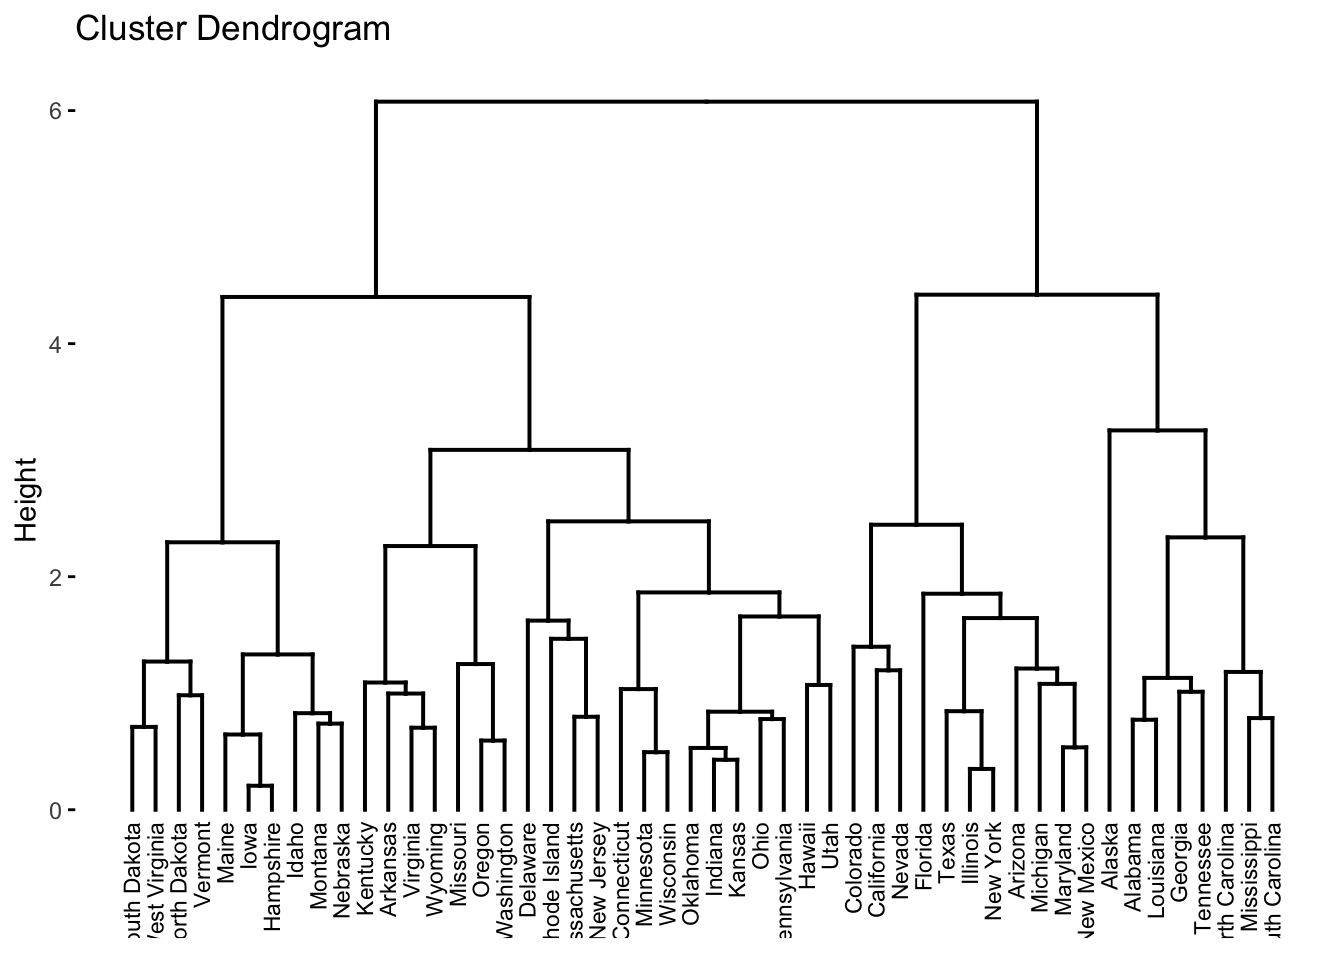
\includegraphics{_main_files/figure-latex/unnamed-chunk-160-1.pdf}

Pode-se utilizar a função \texttt{fviz\_dend} para colorir um número arbitrário de grupos. Note que os grupamentos são obtidos de cima pra baixo, dependente dos valores de \emph{height} (distâncias cofenéticas).

\begin{Shaded}
\begin{Highlighting}[]
\KeywordTok{fviz\_dend}\NormalTok{(hc, }\DataTypeTok{k =} \DecValTok{2}\NormalTok{,  }\CommentTok{\# 2 grupos}
          \DataTypeTok{cex =} \FloatTok{0.6}\NormalTok{,  }\CommentTok{\# tamanho do texto/rótulo (label)}
          \DataTypeTok{rect =} \OtherTok{TRUE} \CommentTok{\# adiciona retângulos ao redor dos grupos}
\NormalTok{)}
\end{Highlighting}
\end{Shaded}

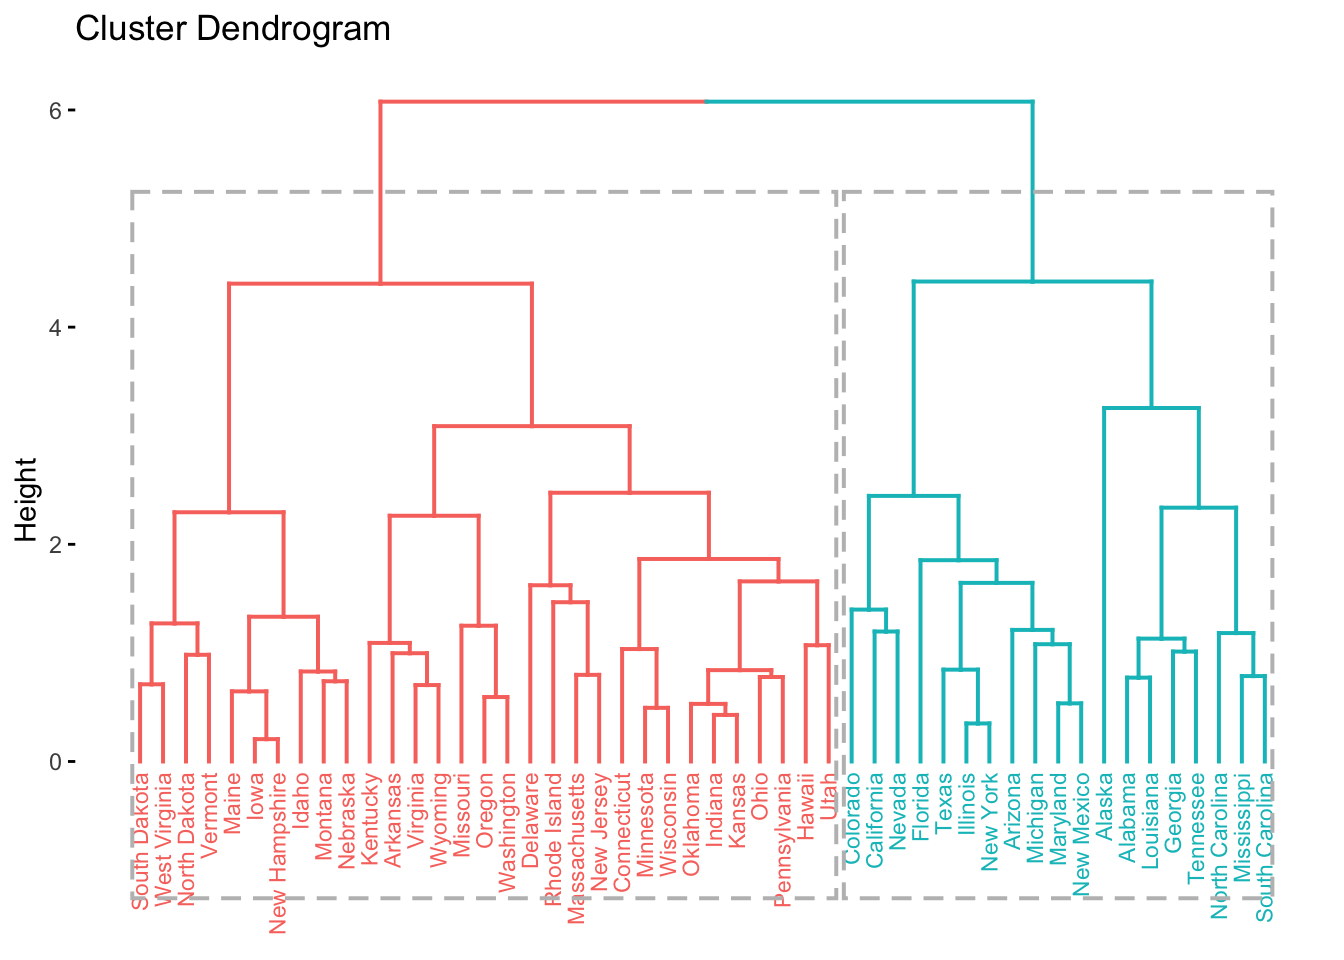
\includegraphics{_main_files/figure-latex/unnamed-chunk-161-1.pdf}

\begin{Shaded}
\begin{Highlighting}[]
\KeywordTok{fviz\_dend}\NormalTok{(hc, }\DataTypeTok{k =} \DecValTok{3}\NormalTok{,  }\CommentTok{\# 3 grupos}
          \DataTypeTok{cex =} \FloatTok{0.6}\NormalTok{,  }\CommentTok{\# tamanho do texto/rótulo (label)}
          \DataTypeTok{rect =} \OtherTok{TRUE} \CommentTok{\# adiciona retângulos ao redor dos grupos}
\NormalTok{)}
\end{Highlighting}
\end{Shaded}

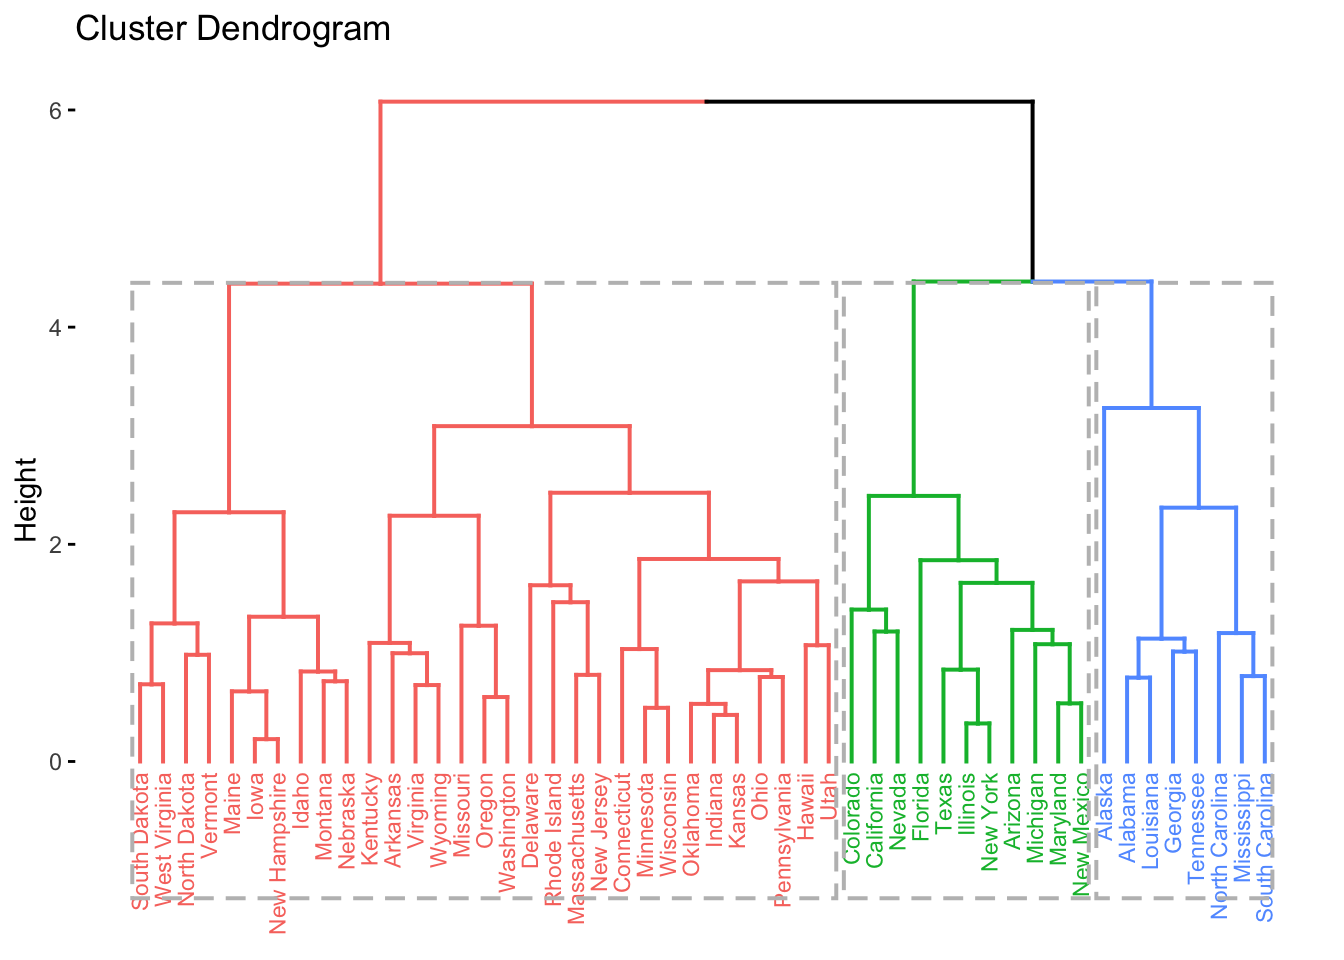
\includegraphics{_main_files/figure-latex/unnamed-chunk-162-1.pdf}

\begin{Shaded}
\begin{Highlighting}[]
\KeywordTok{fviz\_dend}\NormalTok{(hc, }\DataTypeTok{k =} \DecValTok{4}\NormalTok{,  }\CommentTok{\# 4 grupos}
          \DataTypeTok{cex =} \FloatTok{0.6}\NormalTok{,  }\CommentTok{\# tamanho do texto/rótulo (label)}
          \DataTypeTok{rect =} \OtherTok{TRUE} \CommentTok{\# adiciona retângulos ao redor dos grupos}
\NormalTok{)}
\end{Highlighting}
\end{Shaded}

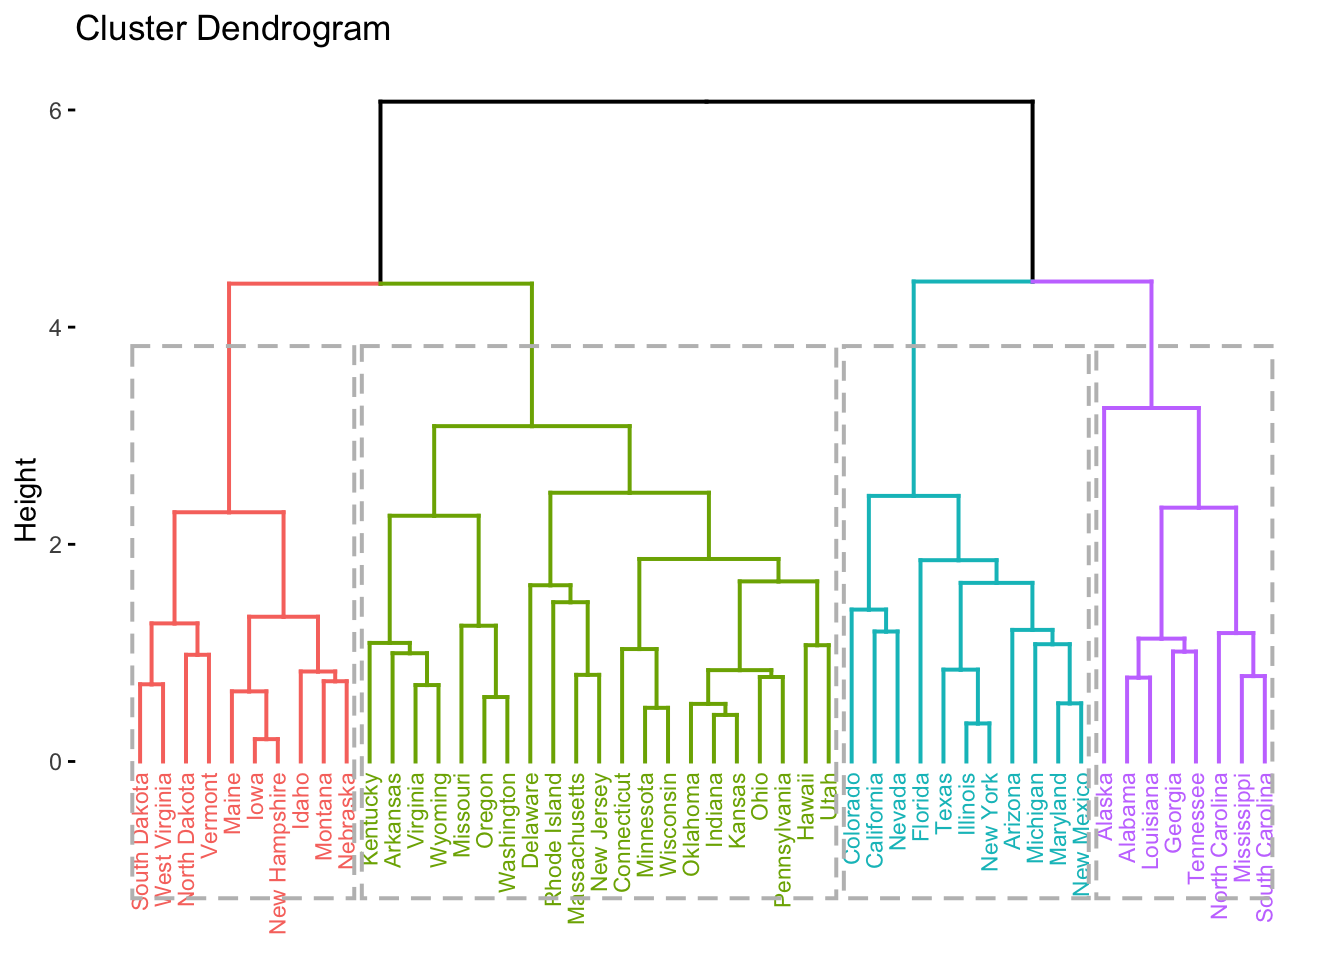
\includegraphics{_main_files/figure-latex/unnamed-chunk-163-1.pdf}

\begin{exercise}
\protect\hypertarget{exr:unnamed-chunk-164}{}{\label{exr:unnamed-chunk-164} }Considere novamente o conjunto de dados \texttt{pib}. Crie dendogramas com a função \texttt{fviz\_dend} utilizando:\\
(a) dados originais e padronizados;\\
(b) diferentes distâncias;\\
(c) diferentes números de grupos.
\end{exercise}

\hypertarget{muxe9todos-nuxe3o-hieruxe1rquicos-de-particionamento}{%
\section{Métodos não hierárquicos (de particionamento)}\label{muxe9todos-nuxe3o-hieruxe1rquicos-de-particionamento}}

\hypertarget{k-muxe9dias}{%
\subsection{K-médias}\label{k-muxe9dias}}

K-médias (\emph{k-means}) é um nome genérico para métodos derivados dos algoritmos de (Lloyd \protect\hyperlink{ref-lloyd1982least}{1957}), (Forgy \protect\hyperlink{ref-forgy1965cluster}{1965}), (MacQueen and others \protect\hyperlink{ref-macqueen1967some}{1967}), (Hartigan \protect\hyperlink{ref-hartigan1975clustering}{1975}) e (Hartigan and Wong \protect\hyperlink{ref-hartigan1979algorithm}{1979}). A ideia básica é encontrar grupos similares, de maneira a minimizar a soma de distâncias euclidianas ao quadrado. As distâncias são calculadas entre os pontos e as médias de cada um dos \(k\) grupos, chamadas \emph{centróides}.

Em relação ao modo de busca podem ser classificados como algoritmos de \emph{comutação}, em que objetos devem ser particionados em \(k\) de grupos. Uma partição inicial é dada de forma arbitrária, onde se definem \(k\) centróides. Calcula-se a distância euclidiana ao quadrado entre as observações e os \(k\) centróides. O centróide mais próximo define o grupo ao qual uma observação pertence. Recalculam-se os novos centróides, e novas partições são obtidas com a alternância dos objetos entre os grupos. O algoritmo encerra quando nenhuma comutação adicional reduz a soma de quadrados intra-grupo, ou quando outro critério de parada é atingido.

São algoritmos relativamente rápidos na execução, mas são afetados pela incerteza da partição inicial. Há sempre a possibilidade de que partições iniciais distintas possam levar a partições finais superiores a outras.

A variação quadrática intra-grupo (\(VQI_{j}\)) do \(j\)-ésimo grupo é dada pela Equação \(\eqref{eq:vqi}\).
\begin{equation}
VQI_{j} = \sum_{x_i \in G_j} (x_i - \mu_j)^2
\label{eq:vqi}
\end{equation}

\begin{itemize}
\tightlist
\item
  \(x_i\) é o \(i\)-ésimo elemento pertencente ao grupo \(G_j\)\\
\item
  \(\mu_j\) é o ponto médio do grupo \(G_j\)\\
\item
  \(j \in \{2, \ldots, k\}\)
\end{itemize}

A soma de quadrados total (\(SQT\)) é dada pela Equação \(\eqref{eq:sqt}\).
\begin{equation}
SQT = \sum_{i=1}^{k} VQI_{i}
\label{eq:sqt}
\end{equation}

Cada observação \(x_i\) é atribuída a um grupo de forma que a \(SQT\) seja mínima a cada iteração. É recomendado que seja feita a padronização dos dados, de maneira a controlar o impacto da escala na definição dos grupos.

\textbf{ALGORITMO DAS K-MÉDIAS}

\begin{quote}
\textbf{PASSO 1} Especifique o número \(k\) de grupos a serem criados.
\end{quote}

\begin{quote}
\textbf{PASSO 2} Selecione arbitrariamente \(k\) pontos como centros dos grupos (centróides).
\end{quote}

\begin{quote}
\textbf{PASSO 3} Atribua cada observação ao grupo de centróide mais próximo, baseado na distância euclidiana entre a observação e os centróides.
\end{quote}

\begin{quote}
\textbf{PASSO 4} Recalcule os centróides com os pontos atribuídos a cada grupo. O centróide do \(j\)-ésimo grupo é um vetor de comprimento \(p\) contendo as médias das \(p\) variáveis, calculadas com todos os pontos atribuídos ao \(j\)-ésimo grupo.
\end{quote}

\begin{quote}
\textbf{PASSO 5} Repita os passos 3 e 4 até que as atribuições não mais reduzam a soma de quadrados intra-grupo, ou que o número máximo de iterações (ou qualquer outro critério de parada) seja atingido.
\end{quote}

\hypertarget{seleuxe7uxe3o-inicial-dos-centruxf3ides}{%
\subsubsection*{Seleção inicial dos centróides}\label{seleuxe7uxe3o-inicial-dos-centruxf3ides}}
\addcontentsline{toc}{subsubsection}{Seleção inicial dos centróides}

(Hartigan \protect\hyperlink{ref-hartigan1975clustering}{1975}) sugere que a seleção inicial dos centróides seja baseada na soma dos casos \(S\), que tem um valor mínimo \(minS\) e um máximo \(maxS\). Para obter \(k\) grupos iniciais, propõe atribuir o \(i\)-ésimo caso ao \(j\)-ésimo grupo, onde \(j\) é a parte inteira de
\begin{equation}
k \left( \dfrac{S-minS}{maxS-minS} \right) + 1
\label{eq:j}
\end{equation}
Uma adaptação será feita, multiplicando 1.01 a \(maxS\) para evitar encontrar \(j>k\).

\begin{Shaded}
\begin{Highlighting}[]
\NormalTok{iris2 \textless{}{-}}\StringTok{ }\KeywordTok{scale}\NormalTok{(iris[}\OperatorTok{{-}}\DecValTok{5}\NormalTok{])}
\NormalTok{S \textless{}{-}}\StringTok{ }\KeywordTok{rowSums}\NormalTok{(iris2)}
\NormalTok{k \textless{}{-}}\StringTok{ }\DecValTok{2}
\NormalTok{zab \textless{}{-}}\StringTok{ }\NormalTok{k}\OperatorTok{*}\NormalTok{(S }\OperatorTok{{-}}\StringTok{ }\KeywordTok{min}\NormalTok{(S))}\OperatorTok{/}\NormalTok{(}\FloatTok{1.01}\OperatorTok{*}\KeywordTok{max}\NormalTok{(S)}\OperatorTok{{-}}\KeywordTok{min}\NormalTok{(S)) }\OperatorTok{+}\StringTok{ }\DecValTok{1} \CommentTok{\# atribuição de Zabala (2019) baseada em Hartigan (1975)}
\NormalTok{(g \textless{}{-}}\StringTok{ }\KeywordTok{floor}\NormalTok{(zab)) }\CommentTok{\# grupos}
\end{Highlighting}
\end{Shaded}

\begin{verbatim}
##   [1] 1 1 1 1 1 1 1 1 1 1 1 1 1 1 1 2 1 1 1 1 1 1 1 1 1 1 1 1 1 1 1 1 1 1 1 1 1 1 1 1 1 1 1 1 1 1 1 1 1 1 2 2 2 1 2 1 2 1 2
##  [60] 1 1 2 1 2 1 2 1 1 1 1 2 1 1 1 2 2 2 2 2 1 1 1 1 2 1 2 2 1 1 1 1 2 1 1 1 1 1 1 1 1 2 2 2 2 2 2 1 2 2 2 2 2 2 1 2 2 2 2
## [119] 2 1 2 2 2 2 2 2 2 2 2 2 2 2 2 2 2 2 2 2 2 2 2 2 2 2 2 2 2 2 2 2
\end{verbatim}

\begin{Shaded}
\begin{Highlighting}[]
\KeywordTok{table}\NormalTok{(g)}
\end{Highlighting}
\end{Shaded}

\begin{verbatim}
## g
##  1  2 
## 83 67
\end{verbatim}

\begin{Shaded}
\begin{Highlighting}[]
\NormalTok{(centroide \textless{}{-}}\StringTok{ }\KeywordTok{by}\NormalTok{(iris2, g, colMeans))}
\end{Highlighting}
\end{Shaded}

\begin{verbatim}
## INDICES: 1
## Sepal.Length  Sepal.Width Petal.Length  Petal.Width 
##      -0.7071       0.0398      -0.6881      -0.7025 
## --------------------------------------------------------------------------------------------- 
## INDICES: 2
## Sepal.Length  Sepal.Width Petal.Length  Petal.Width 
##       0.8759      -0.0494       0.8524       0.8703
\end{verbatim}

\begin{Shaded}
\begin{Highlighting}[]
\KeywordTok{summary}\NormalTok{(iris2)}
\end{Highlighting}
\end{Shaded}

\begin{verbatim}
##   Sepal.Length     Sepal.Width      Petal.Length     Petal.Width    
##  Min.   :-1.864   Min.   :-2.426   Min.   :-1.562   Min.   :-1.442  
##  1st Qu.:-0.898   1st Qu.:-0.590   1st Qu.:-1.222   1st Qu.:-1.180  
##  Median :-0.052   Median :-0.132   Median : 0.335   Median : 0.132  
##  Mean   : 0.000   Mean   : 0.000   Mean   : 0.000   Mean   : 0.000  
##  3rd Qu.: 0.672   3rd Qu.: 0.557   3rd Qu.: 0.760   3rd Qu.: 0.788  
##  Max.   : 2.484   Max.   : 3.080   Max.   : 1.780   Max.   : 1.706
\end{verbatim}

\begin{exercise}
\protect\hypertarget{exr:unnamed-chunk-166}{}{\label{exr:unnamed-chunk-166} }Utilize a Equação (23) sem a correção de Zabala e observe o resultado em \texttt{iris2}.
\end{exercise}

\begin{exercise}
\protect\hypertarget{exr:unnamed-chunk-167}{}{\label{exr:unnamed-chunk-167} }Utilize a Equação (23) com a correção de Zabala para criar uma função que defina os centróides iniciais para um valor genérico \(k\) de grupos em uma base de dados numérica. Teste em \texttt{iris2} e outros bancos de dados já trabalhados.
\end{exercise}

\hypertarget{implementando-no-r}{%
\subsubsection*{Implementando no R}\label{implementando-no-r}}
\addcontentsline{toc}{subsubsection}{Implementando no R}

No R pode-se utilizar a função \texttt{stats::kmeans} para definir os grupamentos através das k-médias. Por padrão, esta função utiliza 10 como valor padrão para o número máximo de iterações e inicia com \(k\) centróides aleatórios.

\begin{Shaded}
\begin{Highlighting}[]
\NormalTok{km \textless{}{-}}\StringTok{ }\ControlFlowTok{function}\NormalTok{(dados,grupos)\{}
\NormalTok{  k \textless{}{-}}\StringTok{ }\KeywordTok{kmeans}\NormalTok{(dados,grupos)}
  \KeywordTok{print}\NormalTok{(}\KeywordTok{table}\NormalTok{(iris}\OperatorTok{$}\NormalTok{Species, k}\OperatorTok{$}\NormalTok{cluster))}
  \KeywordTok{plot}\NormalTok{(dados, }\DataTypeTok{col=}\NormalTok{k}\OperatorTok{$}\NormalTok{cluster)}
\NormalTok{\}}
\KeywordTok{km}\NormalTok{(iris2,}\DecValTok{2}\NormalTok{)}
\end{Highlighting}
\end{Shaded}

\begin{verbatim}
##             
##               1  2
##   setosa     50  0
##   versicolor  0 50
##   virginica   0 50
\end{verbatim}

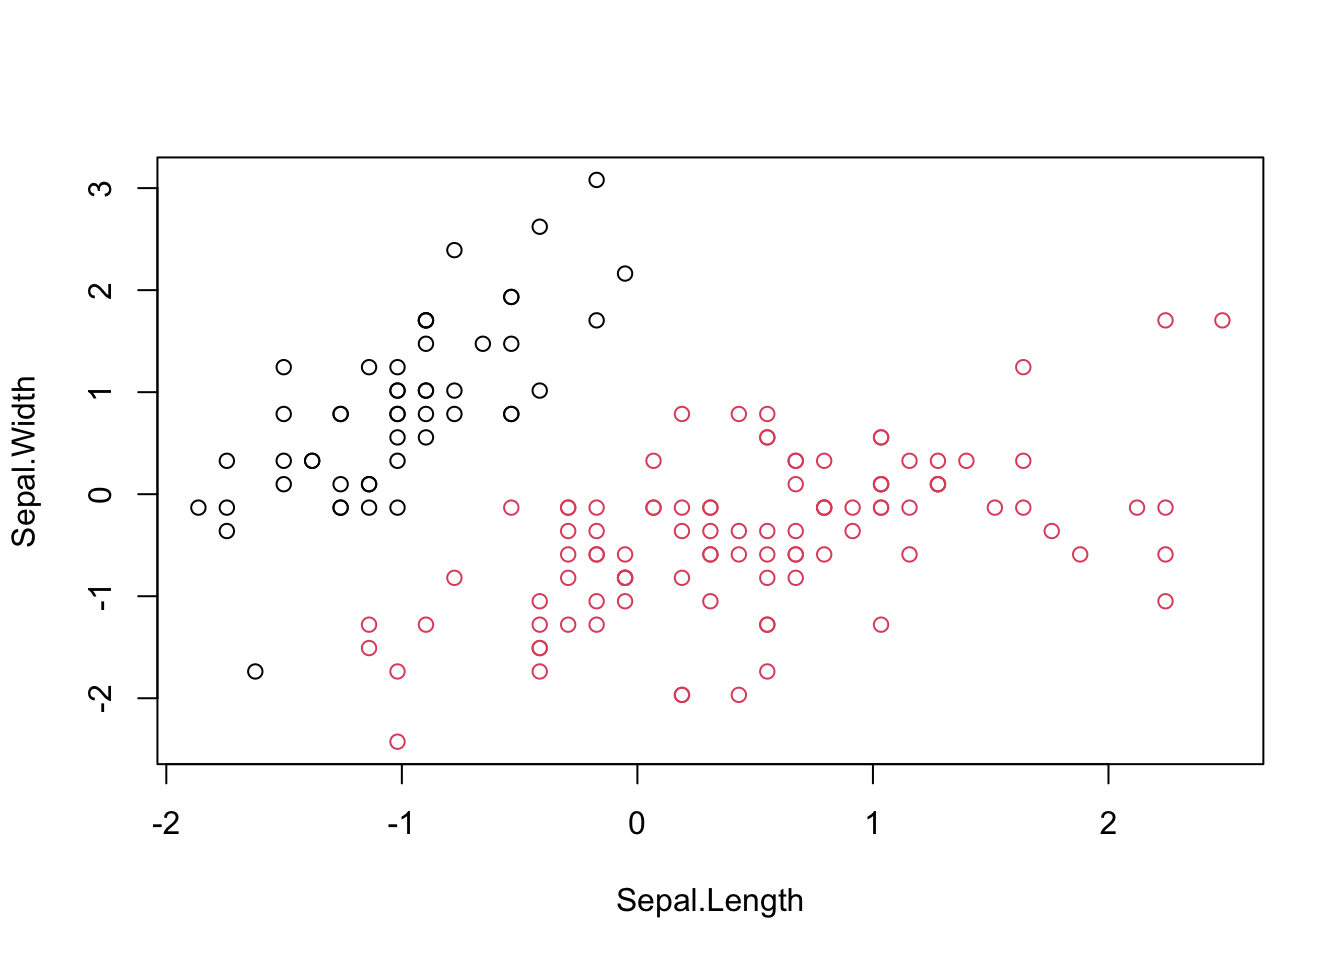
\includegraphics{_main_files/figure-latex/unnamed-chunk-168-1.pdf}

\begin{Shaded}
\begin{Highlighting}[]
\KeywordTok{km}\NormalTok{(iris2,}\DecValTok{3}\NormalTok{)}
\end{Highlighting}
\end{Shaded}

\begin{verbatim}
##             
##               1  2  3
##   setosa      0 33 17
##   versicolor 46  0  4
##   virginica  50  0  0
\end{verbatim}

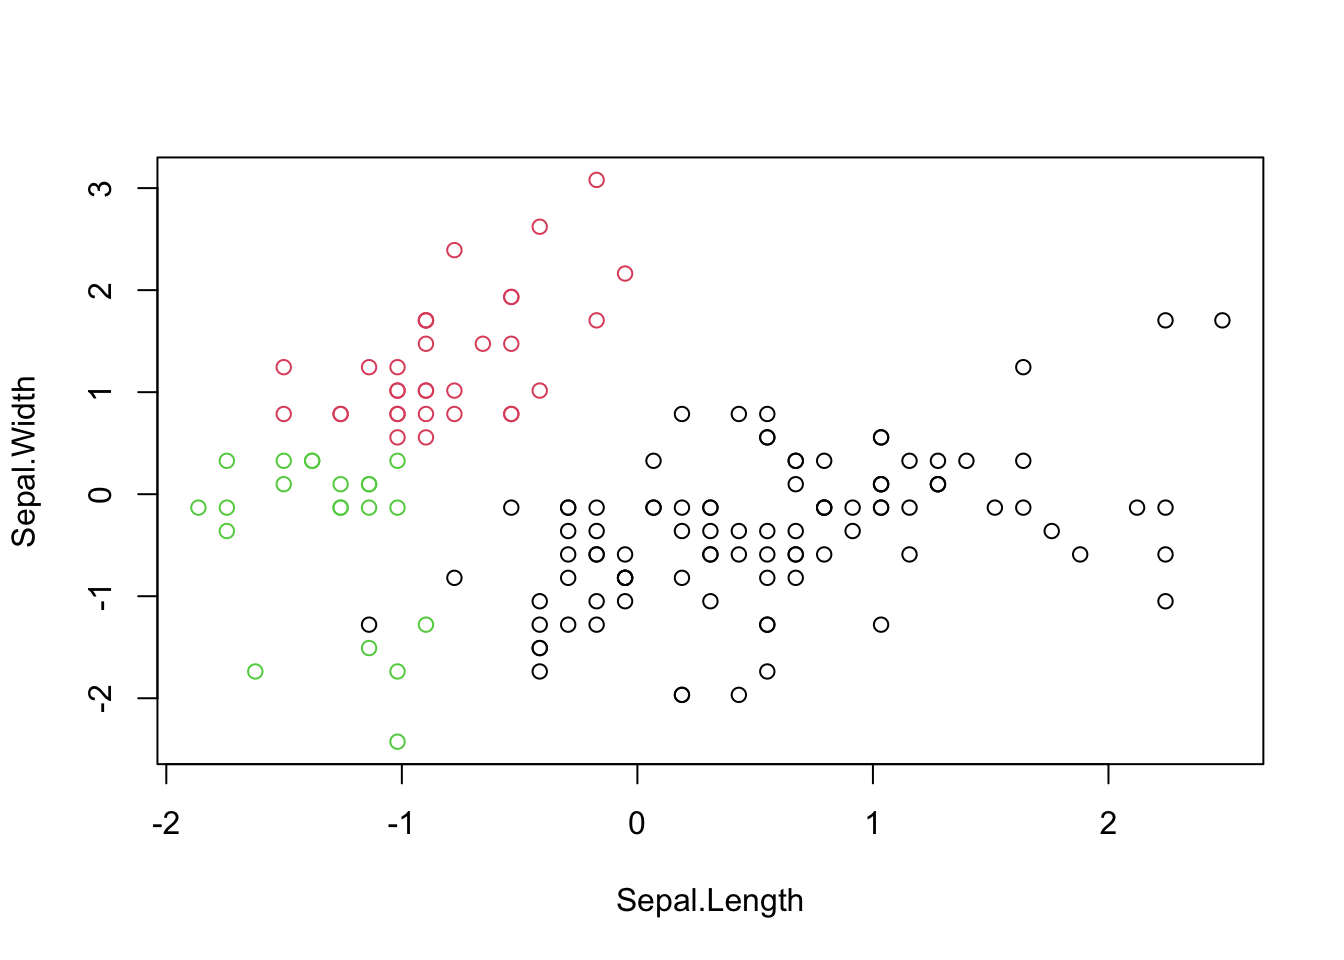
\includegraphics{_main_files/figure-latex/unnamed-chunk-168-2.pdf}

\begin{Shaded}
\begin{Highlighting}[]
\KeywordTok{km}\NormalTok{(iris2,}\DecValTok{4}\NormalTok{)}
\end{Highlighting}
\end{Shaded}

\begin{verbatim}
##             
##               1  2  3  4
##   setosa      0 16 34  0
##   versicolor 11  0  0 39
##   virginica  36  0  0 14
\end{verbatim}

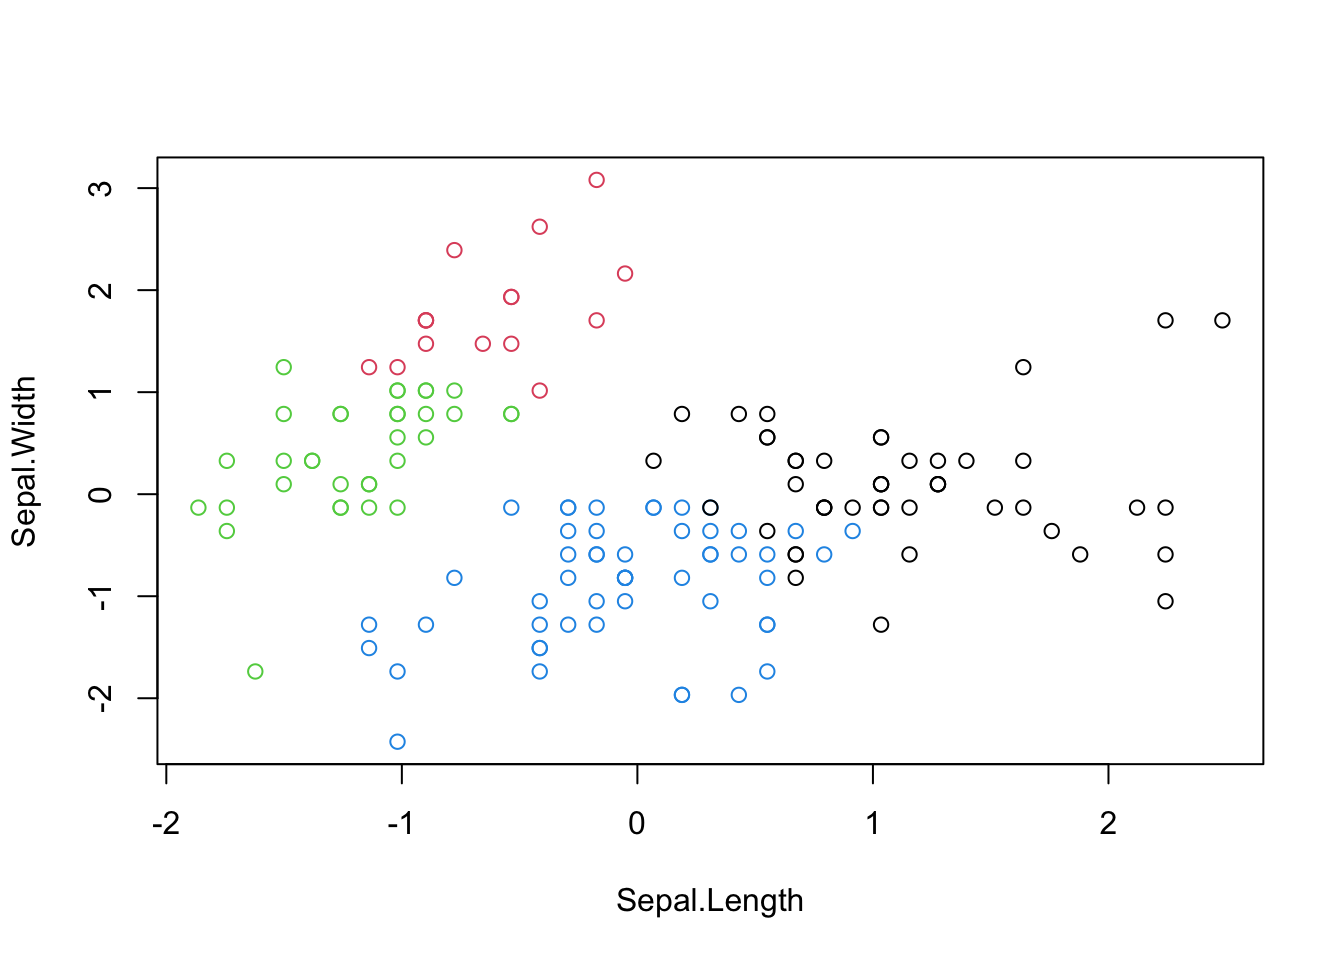
\includegraphics{_main_files/figure-latex/unnamed-chunk-168-3.pdf}

O pacote \texttt{factoextra} fornece uma série de melhorias para a análise de k-means. Além de gráficos mais sofisticados utilizando \texttt{ggplot2}, associa métodos hierárquicos e métodos de particionamento.

\begin{Shaded}
\begin{Highlighting}[]
\NormalTok{km2 \textless{}{-}}\StringTok{ }\ControlFlowTok{function}\NormalTok{(dados,grupos)\{}
\NormalTok{  k \textless{}{-}}\StringTok{ }\KeywordTok{kmeans}\NormalTok{(dados,grupos)}
  \KeywordTok{fviz\_cluster}\NormalTok{(k, iris2, }\DataTypeTok{repel =}\NormalTok{ T)}
\NormalTok{\}}
\KeywordTok{km2}\NormalTok{(iris2,}\DecValTok{2}\NormalTok{)}
\end{Highlighting}
\end{Shaded}

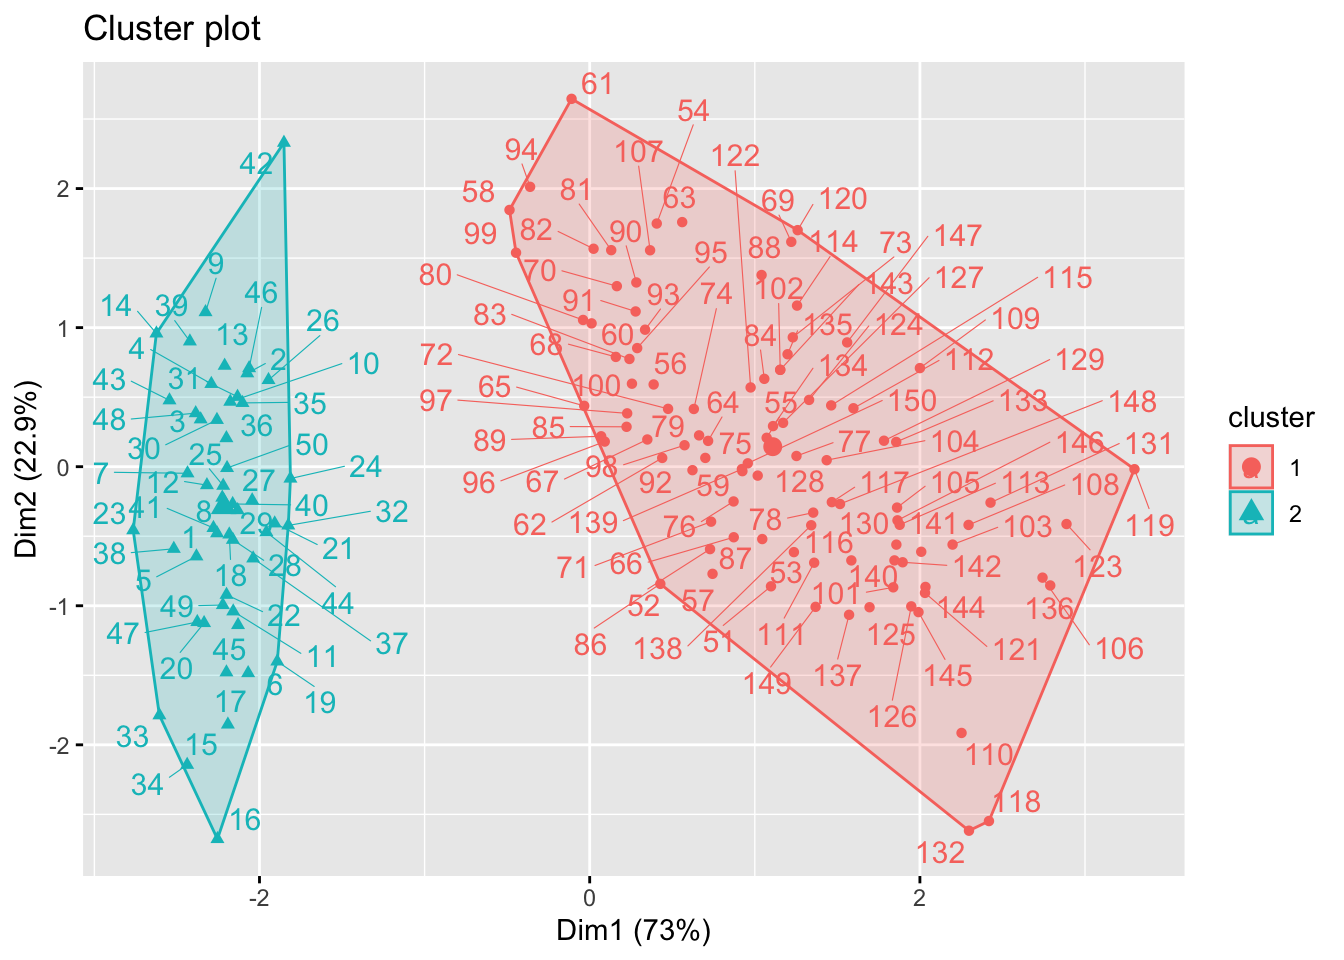
\includegraphics{_main_files/figure-latex/unnamed-chunk-169-1.pdf}

\begin{Shaded}
\begin{Highlighting}[]
\KeywordTok{km2}\NormalTok{(iris2,}\DecValTok{3}\NormalTok{)}
\end{Highlighting}
\end{Shaded}

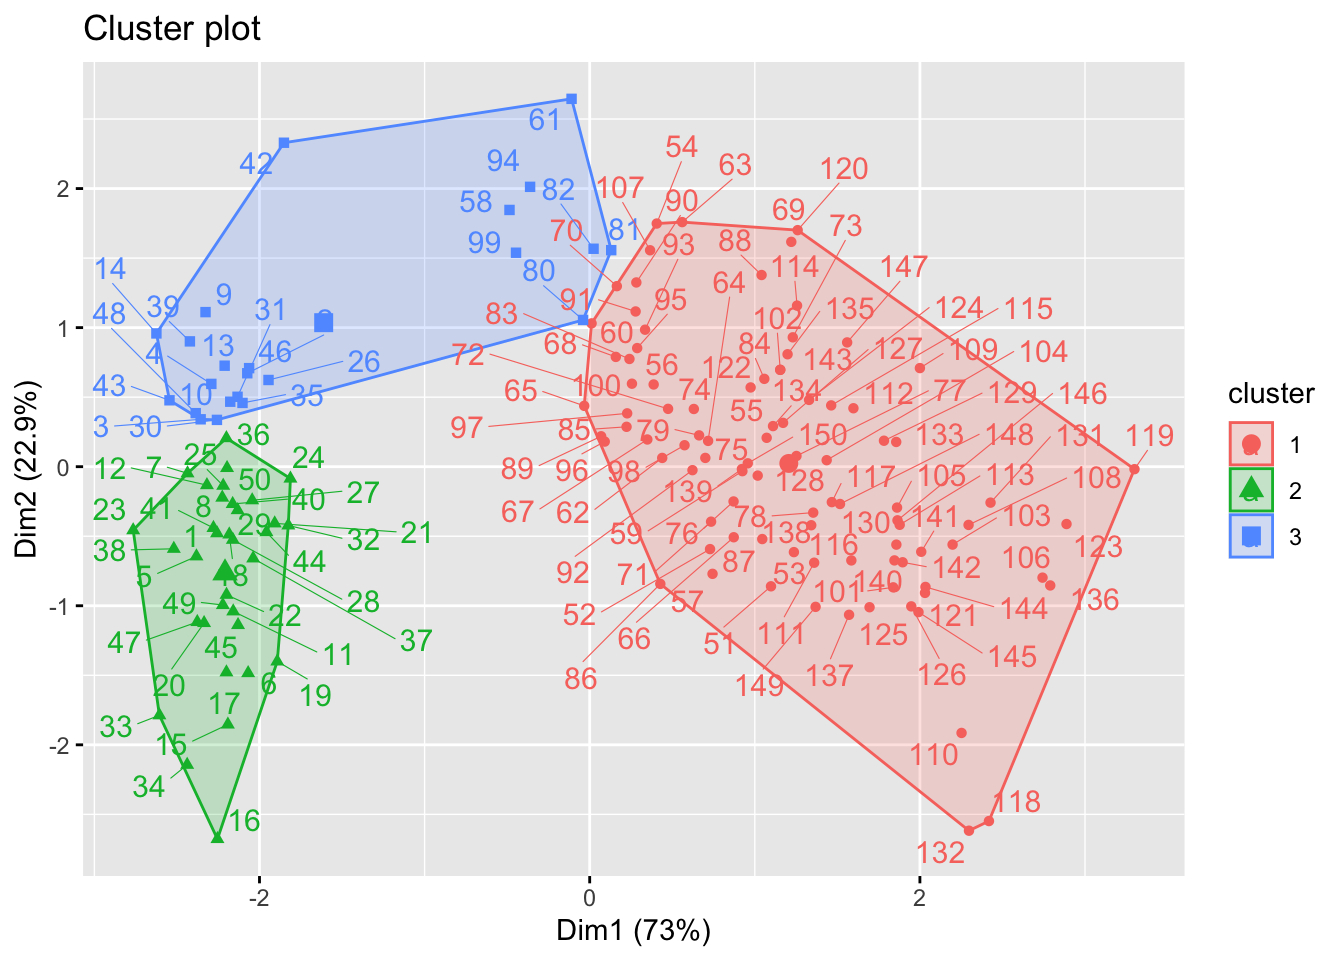
\includegraphics{_main_files/figure-latex/unnamed-chunk-169-2.pdf}

\begin{Shaded}
\begin{Highlighting}[]
\KeywordTok{km2}\NormalTok{(iris2,}\DecValTok{4}\NormalTok{)}
\end{Highlighting}
\end{Shaded}

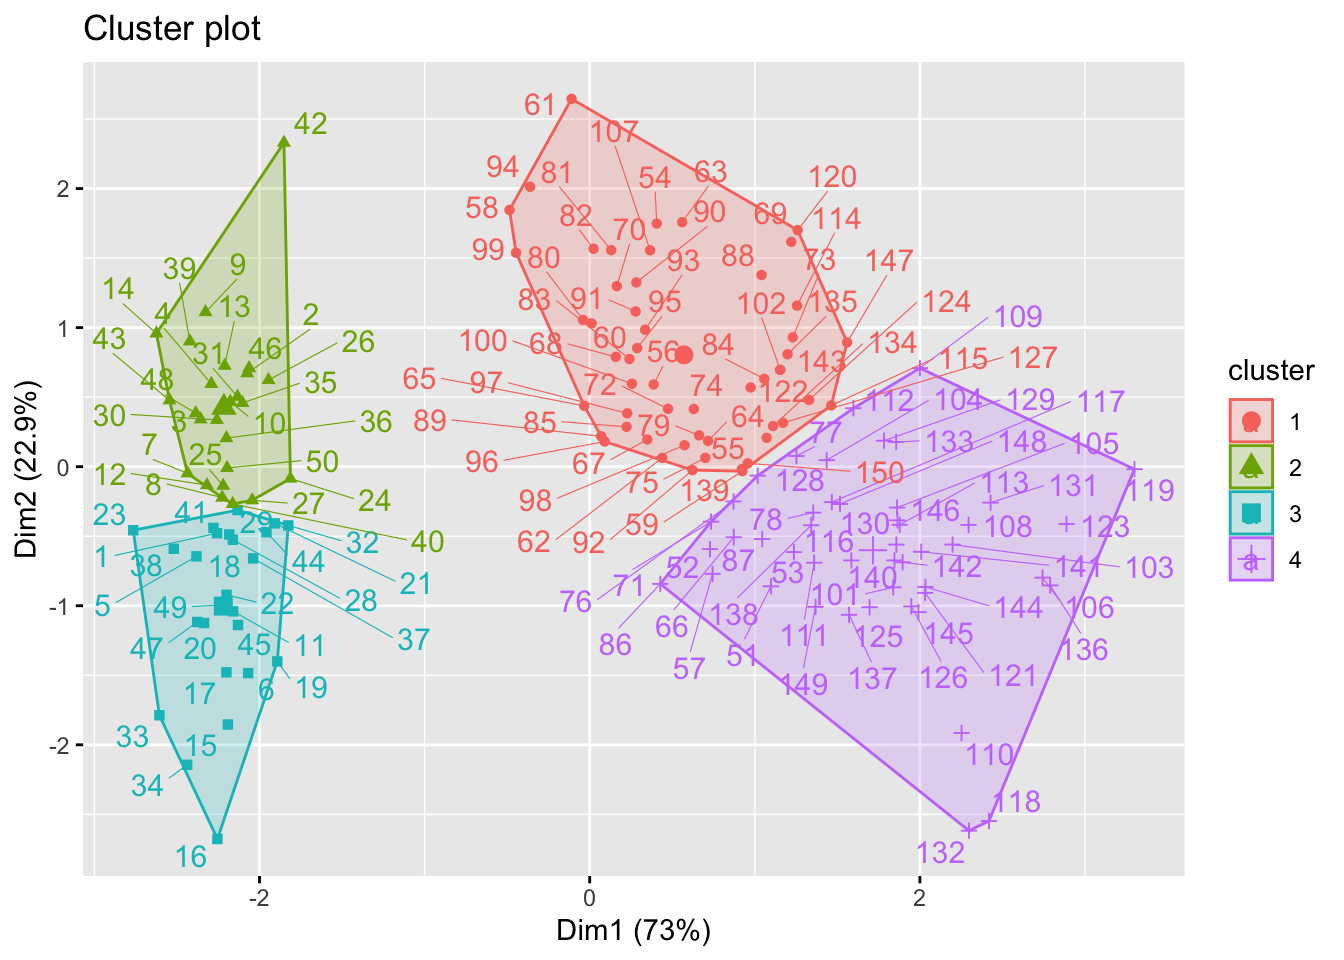
\includegraphics{_main_files/figure-latex/unnamed-chunk-169-3.pdf}

\hypertarget{nuxfamero-de-grupos}{%
\subsubsection*{Número de grupos}\label{nuxfamero-de-grupos}}
\addcontentsline{toc}{subsubsection}{Número de grupos}

A função \texttt{factoextra::fviz\_nbclust} fornece métodos para a escolha de um número ótimo de grupos. O método \texttt{wss} (\emph{total \textbf{w}ithin \textbf{s}um of \textbf{s}quare}), busca um número de grupos que traga um bom custo-benefício entre o número de grupos (\(k\)) e a soma de quadrados total (\(SQT\)). Este custo-benefício é indicado onde a curva muda sua declividade, ou no `cotovelo' (\emph{elbow}) do gráfico de \(k\) por \(SQT\). Tem suas origens no trabalho de (Thorndike \protect\hyperlink{ref-thorndike1953belongs}{1953}).

\begin{Shaded}
\begin{Highlighting}[]
\KeywordTok{fviz\_nbclust}\NormalTok{(iris2, kmeans, }\DataTypeTok{method =} \StringTok{\textquotesingle{}wss\textquotesingle{}}\NormalTok{)}
\end{Highlighting}
\end{Shaded}

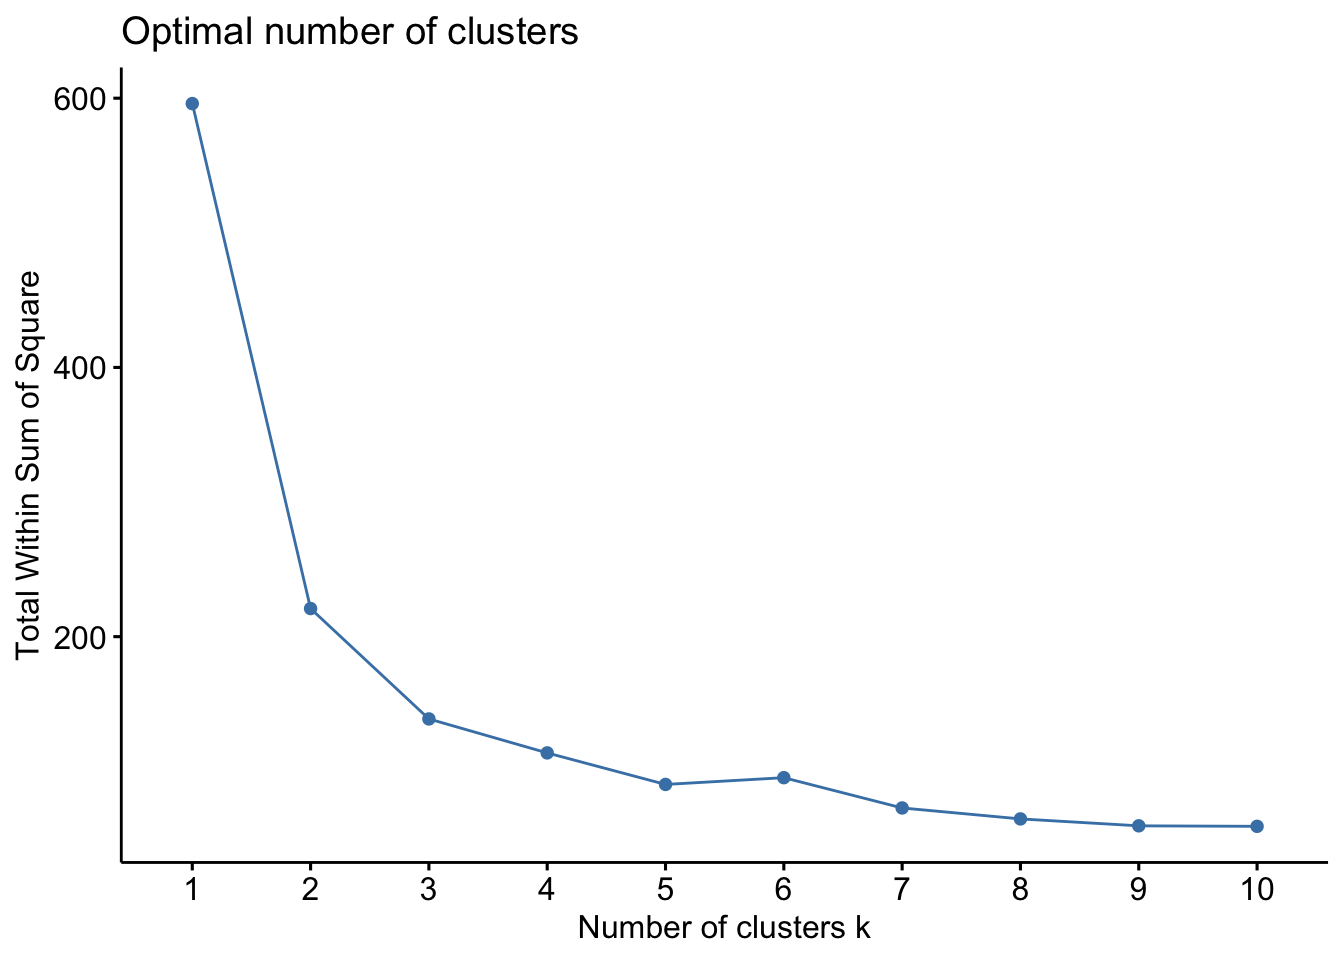
\includegraphics{_main_files/figure-latex/unnamed-chunk-170-1.pdf}

O método \texttt{silhouette} busca o número de grupos que maximize o tamanho médio da silhueta. É baseado em uma medida sugerida por (Rousseeuw and Kaufman \protect\hyperlink{ref-rousseeuw1990finding}{1990}), dada por
\begin{equation}
s(i) = \dfrac{b(i)-a(i)}{max\{ a(i),b(i) \}}
\label{eq:silhueta}
\end{equation}
- \(-1 \le s(i) \le 1\)\\
- \(a(i)\): dissimilaridade média do elemento \(i\) em relação a todos os demais elementos do seu grupo \(A\)\\
- \(d(i,C)\): dissimilaridade média do elemento \(i\) em relação a todos os elementos do grupo \(C \ne A\)\\
- \(b(i) = \underset{C \ne A}{\mathrm{min}} \; d(i,C)\)

\begin{Shaded}
\begin{Highlighting}[]
\KeywordTok{fviz\_nbclust}\NormalTok{(iris2, kmeans, }\DataTypeTok{method =} \StringTok{\textquotesingle{}silhouette\textquotesingle{}}\NormalTok{)}
\end{Highlighting}
\end{Shaded}

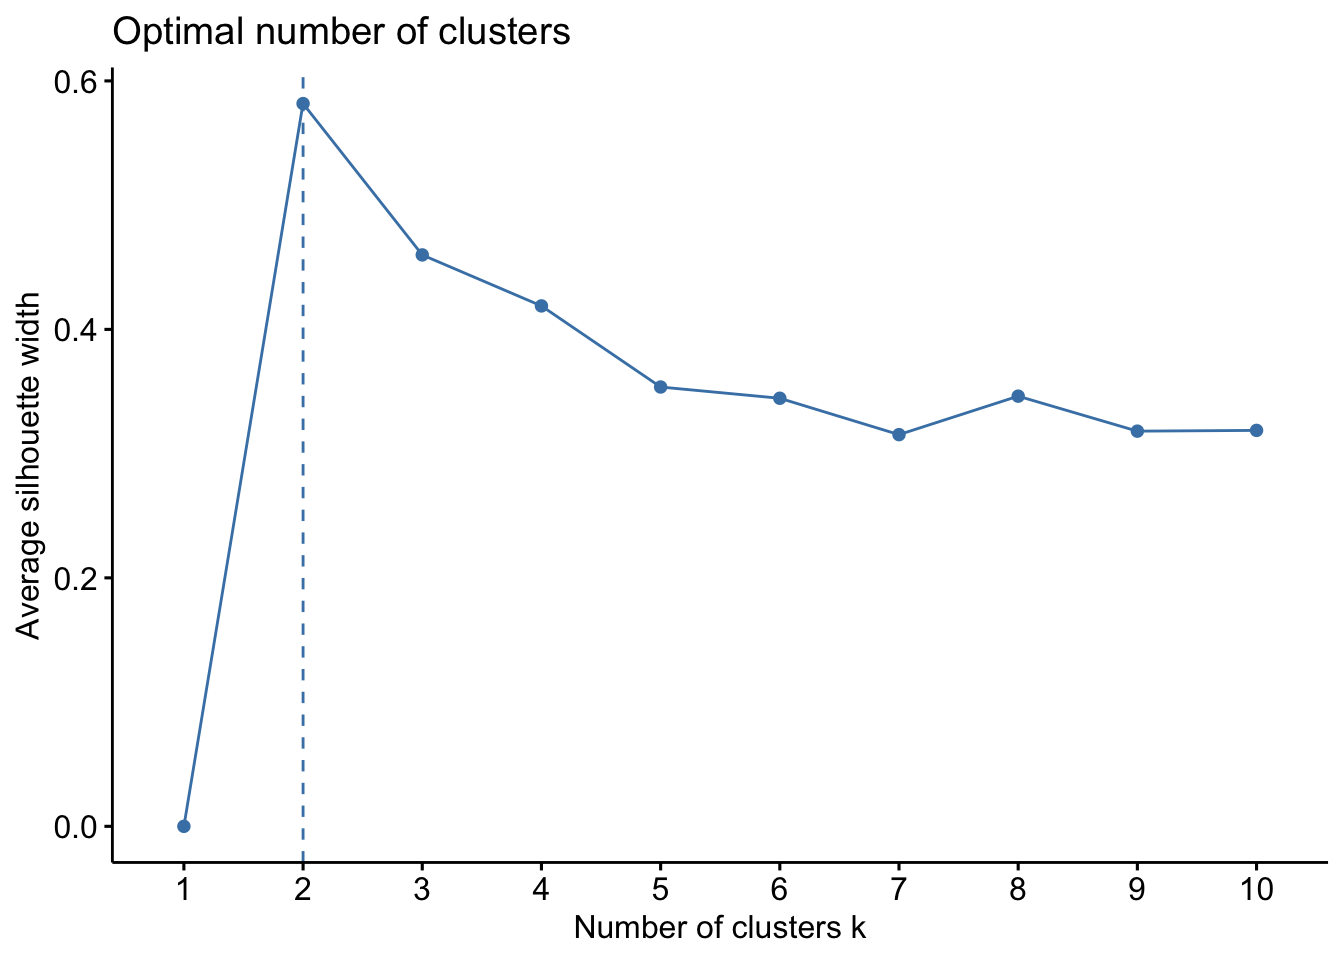
\includegraphics{_main_files/figure-latex/unnamed-chunk-171-1.pdf}

Proposto por (Tibshirani, Walther, and Hastie \protect\hyperlink{ref-tibshirani2001estimating}{2001}), o método \texttt{gap\_stat} (\emph{gap statistic}) compara variação total intra-grupo para diferentes valores de k com seus valores esperados sob alguma distribuição de referência. A estimativa dos clusters ótimos será o valor que maximiza a estatística de gap (isto é, que gera a maior estatística de gap).
\begin{equation}
\mathrm{Gap}_{n}(k) = E^{*} \{ \mathrm{log}(W_k) \} - \mathrm{log}(W_k)
\label{eq:gap}
\end{equation}
- \(E^{*}\) é o valor esperado sob uma amostra de tamanho \(n\) da distribuição de referência\\
- \(W_k = \sum_{j=1}^{k} \dfrac{1}{2n_j} D_j\)\\
- \(D_j = \sum_{i,i' \in C_j} d_{ii'}\)\\
- \(n_j = |C_j|\)

\begin{Shaded}
\begin{Highlighting}[]
\KeywordTok{fviz\_nbclust}\NormalTok{(iris2, kmeans, }\DataTypeTok{method =} \StringTok{\textquotesingle{}gap\_stat\textquotesingle{}}\NormalTok{)}
\end{Highlighting}
\end{Shaded}

\begin{verbatim}
## Clustering k = 1,2,..., K.max (= 10): .. done
## Bootstrapping, b = 1,2,..., B (= 100)  [one "." per sample]:
## .................................................. 50 
## .................................................. 100
\end{verbatim}

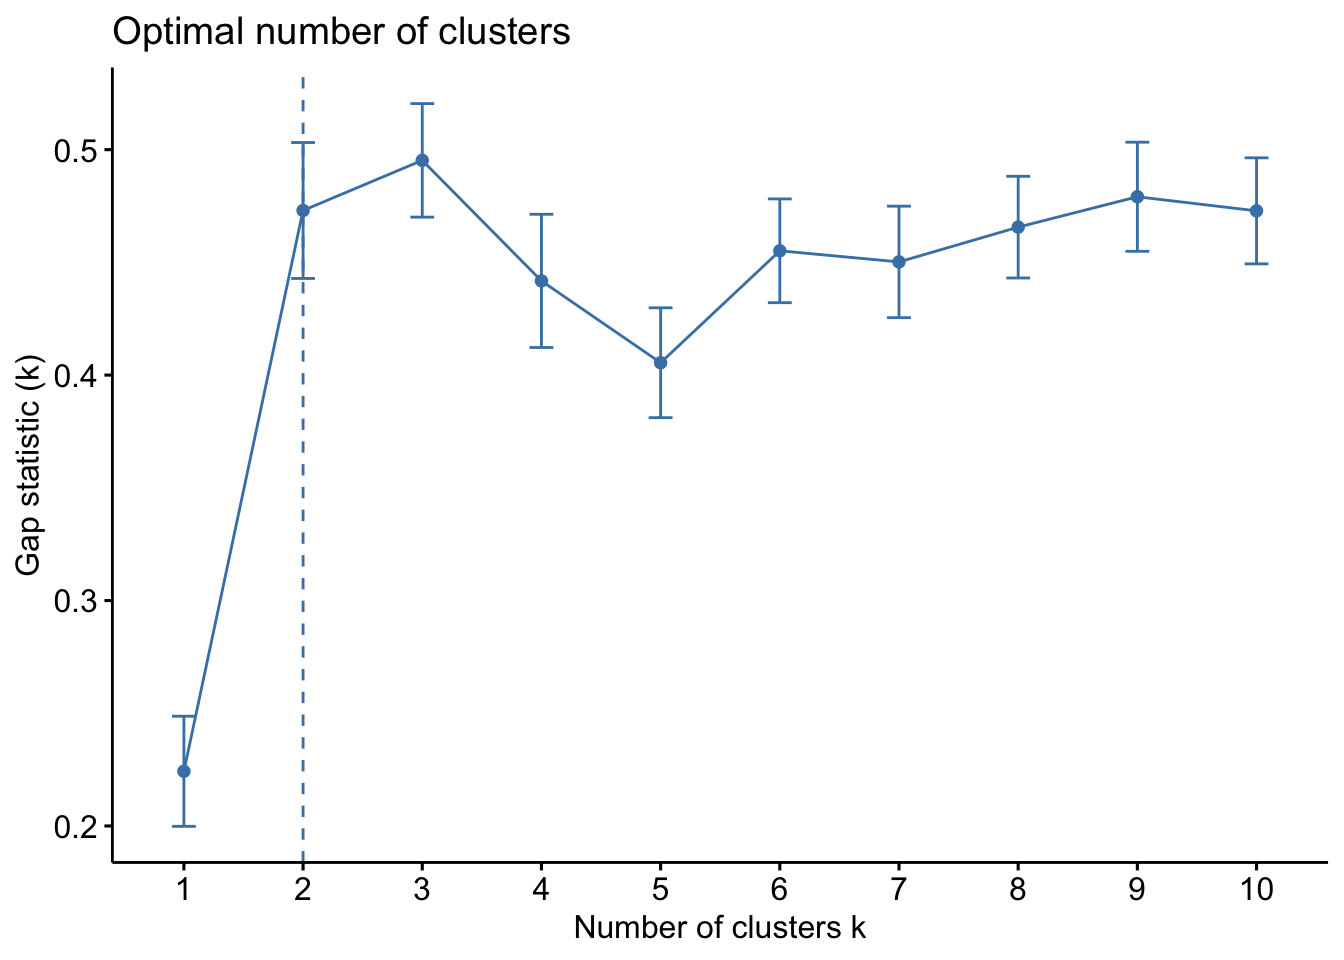
\includegraphics{_main_files/figure-latex/unnamed-chunk-172-1.pdf}

\begin{exercise}
\protect\hypertarget{exr:unnamed-chunk-173}{}{\label{exr:unnamed-chunk-173} }Leia:\\
(a) a documentação da função \texttt{fviz\_nbclust}.\\
(b) \url{https://www.datanovia.com/en/lessons/determining-the-optimal-number-of-clusters-3-must-know-methods}.\\
(c) A Seção \emph{e. Graphical Output Concerning Each Clustering}, pg. 83-88 de (Rousseeuw and Kaufman \protect\hyperlink{ref-rousseeuw1990finding}{1990}).
\end{exercise}

\begin{exercise}
\protect\hypertarget{exr:unnamed-chunk-174}{}{\label{exr:unnamed-chunk-174} }Considere novamente o conjunto de dados \texttt{pib}.\\
(a) Verifique as sugestões do número ótimo de grupos com os diferente métodos disponíveis na função \texttt{fviz\_nbclust}.\\
(b) Crie o grupamento que considerar mais adequado aos dados e apresente com a função \texttt{fviz\_cluster}.\\
(c) Compare os resultados com o Exercício 7.3.
\end{exercise}

\begin{exercise}
\protect\hypertarget{exr:unnamed-chunk-175}{}{\label{exr:unnamed-chunk-175} }Considere o conjunto de dados \texttt{drinks}, discutido no Capítulo 5.\\
(a) Calcule as distâncias de Manhattan, euclidiana e de Minkowski com \(p=3\).\\
(b) Obtenha os modelos hierárquicos utilizando as três distâncias do item (a). Você nota alguma diferença?\\
(c) Obtenha a seleção inicial dos centróides a partir de proposta de (Hartigan \protect\hyperlink{ref-hartigan1975clustering}{1975}) apresentada na Equação \(\eqref{eq:j}\). Sugestão: escreva uma função que dependa dos dados e de \(k\), realizando alguma correção que considerar relevante.\\
(d) Calcule os centróides dos grupos obtidos no item (c).\\
(e) Calcule a \(VQI\) dos grupos obtidos no item (c) a partir da Eq. \(\eqref{eq:vqi}\).\\
(f) Calcule a \(SQT\) dos grupos obtidos no item (c) a partir da Eq. \(\eqref{eq:sqt}\).\\
(g) Verifique as sugestões do número ótimo de grupos com os diferente métodos disponíveis na função \texttt{fviz\_nbclust}.\\
(h) Crie o grupamento que considerar mais adequado aos dados e apresente com a função \texttt{fviz\_cluster}.\\
\end{exercise}

\begin{Shaded}
\begin{Highlighting}[]
\NormalTok{dat \textless{}{-}}\StringTok{ }\KeywordTok{read.table}\NormalTok{(}\StringTok{\textquotesingle{}http://www.filipezabala.com/data/drinks.txt\textquotesingle{}}\NormalTok{, }\DataTypeTok{header =}\NormalTok{ T, }\DataTypeTok{sep =} \StringTok{\textquotesingle{}}\CharTok{\textbackslash{}t}\StringTok{\textquotesingle{}}\NormalTok{)}
\end{Highlighting}
\end{Shaded}

\begin{exercise}
\protect\hypertarget{exr:unnamed-chunk-177}{}{\label{exr:unnamed-chunk-177} }Considere o banco de dados sobre eficiência energética didcutido no Exemplo 5.2.\\
(a) Calcule as distâncias de Manhattan, euclidiana e de Minkowski com \(p=3\).\\
(b) Obtenha os modelos hierárquicos utilizando as três distâncias do item (a). (PODE DEMORAR!)\\
(c) Verifique as sugestões do número ótimo de grupos com os diferente métodos disponíveis na função \texttt{fviz\_nbclust}.\\
(d) Crie o grupamento que considerar mais adequado aos dados e apresente com a função \texttt{fviz\_cluster}.\\
\end{exercise}

\begin{Shaded}
\begin{Highlighting}[]
\KeywordTok{library}\NormalTok{(readxl)}
\NormalTok{url1 \textless{}{-}}\StringTok{ \textquotesingle{}http://archive.ics.uci.edu/ml/machine{-}learning{-}databases/00242/ENB2012\_data.xlsx\textquotesingle{}}
\KeywordTok{download.file}\NormalTok{(url1, }\StringTok{\textquotesingle{}temp.xlsx\textquotesingle{}}\NormalTok{, }\DataTypeTok{mode =} \StringTok{\textquotesingle{}wb\textquotesingle{}}\NormalTok{)}
\NormalTok{dat \textless{}{-}}\StringTok{ }\KeywordTok{read\_excel}\NormalTok{(}\StringTok{\textquotesingle{}temp.xlsx\textquotesingle{}}\NormalTok{)}
\end{Highlighting}
\end{Shaded}

\hypertarget{seriestemporais}{%
\chapter{Séries Temporais}\label{seriestemporais}}

Uma \emph{série temporal} é um conjunto de dados observado no tempo. (Hyndman and Athanasopoulos \protect\hyperlink{ref-hyndman2018forecasting}{2018}) trazem uma compilação dos principais e mais recentes métodos da literatura, programados na biblioteca \texttt{fpp2} de (Hyndman \protect\hyperlink{ref-hyndman2020fpp2}{2020}). A seguir está o código \texttt{fits}, escrito com algumas funções desta biblioteca, de maneira a utilizar os seguintes métodos:

\begin{itemize}
\tightlist
\item
  \href{https://otexts.com/fpp2/arima.html}{ARIMA} (\emph{AutoRegressive Integrated Moving Average}), função \href{https://www.rdocumentation.org/packages/forecast/versions/8.7/topics/auto.arima}{\texttt{auto.arima}}\\
\item
  \href{https://otexts.com/fpp2/ets.html}{ETS} (Modelo de espaço de estados com suavização exponencial), função \href{https://www.rdocumentation.org/packages/forecast/versions/8.7/topics/ets}{\texttt{ets}}\\
\item
  \href{https://otexts.com/fpp2/complexseasonality.html}{TBATS} (Modelo de espaço de estados com suavização exponencial com transformação Box-Cox, erros ARMA e componentes sazonais e de tendência), função \href{https://www.rdocumentation.org/packages/forecast/versions/8.7/topics/tbats}{\texttt{tbats}}\\
\item
  \href{https://otexts.com/fpp2/nnetar.html}{NNETAR} (Rede neural autorregressiva), função \href{https://www.rdocumentation.org/packages/forecast/versions/8.7/topics/nnetar}{\texttt{nnetar}}
\end{itemize}

\begin{Shaded}
\begin{Highlighting}[]
\CommentTok{\# calling package}
\KeywordTok{library}\NormalTok{(jurimetrics)}
\CommentTok{\# example}
\KeywordTok{fits}\NormalTok{(livestock)}
\end{Highlighting}
\end{Shaded}

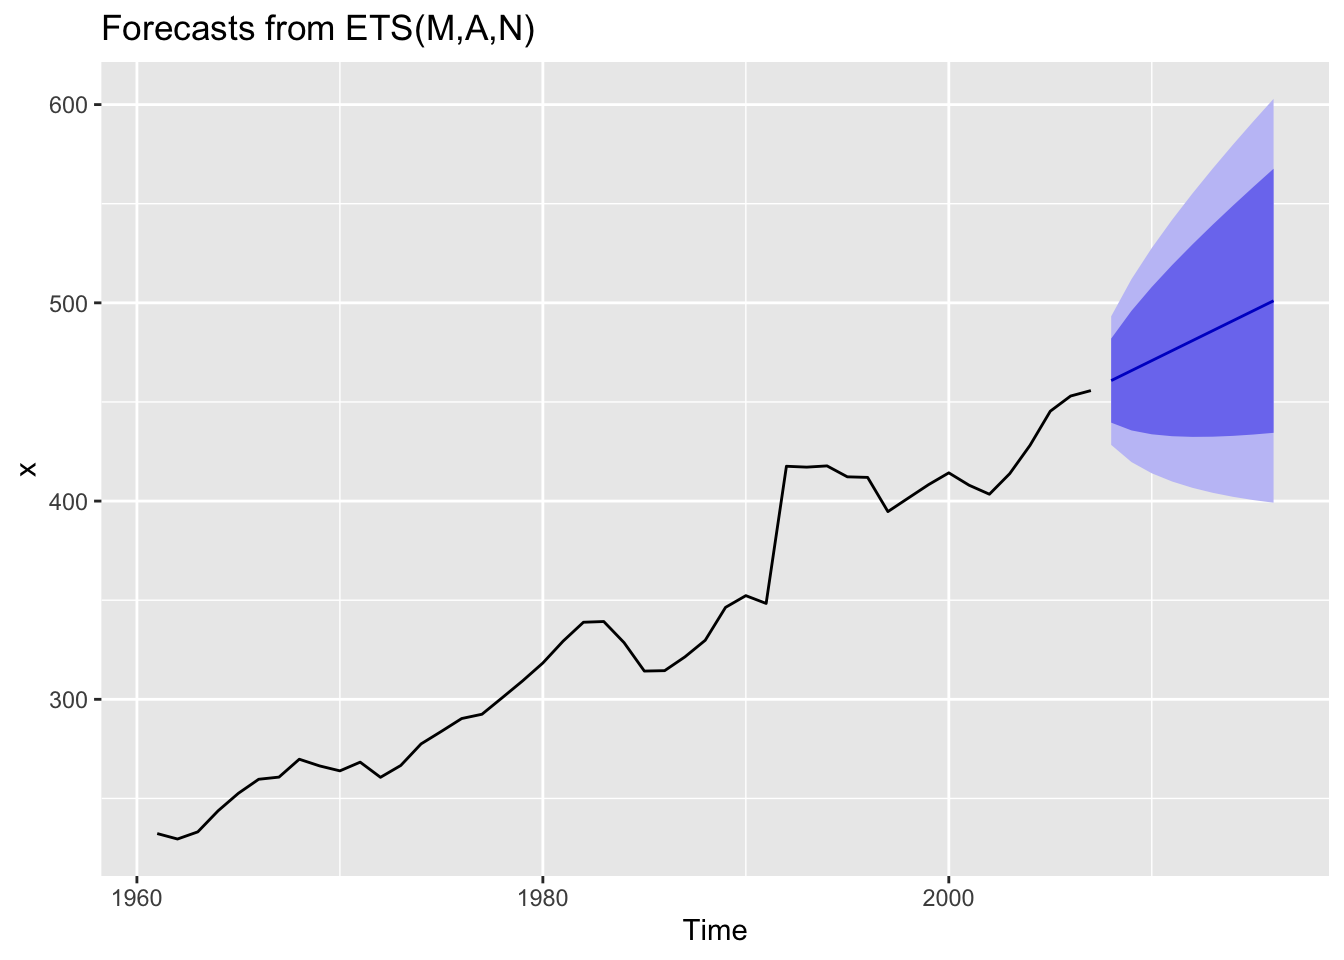
\includegraphics{_main_files/figure-latex/unnamed-chunk-179-1.pdf}

\begin{verbatim}
## $fcast
##      Point Forecast Lo 80 Hi 80 Lo 95 Hi 95
## 2008            461   440   482   428   493
## 2009            466   436   496   420   512
## 2010            471   434   508   414   528
## 2011            476   433   519   410   542
## 2012            481   432   529   407   555
## 2013            486   432   539   404   568
## 2014            491   433   549   402   580
## 2015            496   434   558   401   591
## 2016            501   434   568   399   603
## 
## $mse.pred
##   mse.pred.aa mse.pred.ets mse.pred.tb mse.pred.nn
## 1         109          103         253         742
## 
## $best.model
## [1] "ets"
## 
## $runtime
## Time difference of 1.18 secs
\end{verbatim}

\begin{exercise}
\protect\hypertarget{exr:unnamed-chunk-180}{}{\label{exr:unnamed-chunk-180} }Considere a função \texttt{fits}.\\
a) Avalie os parâmetros da função a partir do código.\\
b) Aplique nos bancos de dados \texttt{h02} e \texttt{gas}, utliizando os parâmetros que considerar mais adequados.\\
\end{exercise}

\begin{exercise}
\protect\hypertarget{exr:unnamed-chunk-181}{}{\label{exr:unnamed-chunk-181} }Considere o banco de dados do índice Dow Jones disponível em \url{https://archive.ics.uci.edu/ml/datasets/Dow+Jones+Index}, lido com o código abaixo.
\end{exercise}

\begin{Shaded}
\begin{Highlighting}[]
\NormalTok{url1 \textless{}{-}}\StringTok{ \textquotesingle{}https://archive.ics.uci.edu/ml/machine{-}learning{-}databases/00312/dow\_jones\_index.zip\textquotesingle{}}
\KeywordTok{download.file}\NormalTok{(url1, }\StringTok{\textquotesingle{}temp.zip\textquotesingle{}}\NormalTok{, }\DataTypeTok{mode =} \StringTok{\textquotesingle{}wb\textquotesingle{}}\NormalTok{)}
\NormalTok{dat \textless{}{-}}\StringTok{ }\KeywordTok{suppressMessages}\NormalTok{(}\KeywordTok{read\_csv}\NormalTok{(}\StringTok{\textquotesingle{}temp.zip\textquotesingle{}}\NormalTok{))}
\NormalTok{st \textless{}{-}}\StringTok{ }\KeywordTok{ts}\NormalTok{(dat}\OperatorTok{$}\NormalTok{percent\_change\_next\_weeks\_price)}
\end{Highlighting}
\end{Shaded}

\begin{enumerate}
\def\labelenumi{\alph{enumi}.}
\tightlist
\item
  Modele e projete a série \texttt{percent\_change\_next\_weeks\_price} através da função \texttt{fits}. Busque pelos melhores modelos alterando os parâmetros da função, tais como \texttt{train} e \texttt{max.points}.\\
\item
  Avalie outras colunas do banco de dados e repita as operações do item a.
\end{enumerate}

\hypertarget{impacto-causal}{%
\section{Impacto Causal}\label{impacto-causal}}

\begin{itemize}
\tightlist
\item
  \url{http://google.github.io/CausalImpact/CausalImpact.html}
\item
  \url{https://research.google/pubs/pub41854/}
\item
  \url{https://github.com/klarsen1/MarketMatching}
\end{itemize}

\hypertarget{referuxeancias}{%
\chapter{Referências}\label{referuxeancias}}

\hypertarget{refs}{}
\begin{cslreferences}
\leavevmode\hypertarget{ref-agresti2007introduction}{}%
Agresti, Alan. 2007. \emph{An Introduction to Categorical Data Analysis}. Wiley. \url{https://mregresion.files.wordpress.com/2012/08/agresti-introduction-to-categorical-data.pdf}.

\leavevmode\hypertarget{ref-akaike1974new}{}%
Akaike, Hirotugu. 1974. ``A New Look at the Statistical Model Identification.'' In \emph{Selected Papers of Hirotugu Akaike}, 215--22. Springer.

\leavevmode\hypertarget{ref-bayes1763essay}{}%
Bayes, Thomas. 1763. ``An Essay Towards Solving a Problem in the Doctrine of Chances. By the Late Rev. Mr. Bayes, FRS Communicated by Mr. Price, in a Letter to John Canton, AMFR S.'' \emph{Philosophical Transactions of the Royal Society of London}, no. 53: 370--418. \url{https://www.ias.ac.in/article/fulltext/reso/008/04/0080-0088}.

\leavevmode\hypertarget{ref-beasley1995multiple}{}%
Beasley, T Mark, and Randall E Schumacker. 1995. ``Multiple Regression Approach to Analyzing Contingency Tables: Post Hoc and Planned Comparison Procedures.'' \emph{The Journal of Experimental Education} 64 (1): 79--93.

\leavevmode\hypertarget{ref-berger1985statistical}{}%
Berger, James O. 1985. \emph{Statistical Decision Theory and Bayesian Analysis}. 2nd ed. Springer Science \& Business Media. \url{https://www.springer.com/gp/book/9780387960982}.

\leavevmode\hypertarget{ref-birnbaum1962foundations}{}%
Birnbaum, Allan. 1962. ``On the Foundations of Statistical Inference.'' \emph{Journal of the American Statistical Association} 57 (298): 269--306. \url{https://www.jstor.org/stable/2281640}.

\leavevmode\hypertarget{ref-bishop1999bayesian}{}%
Bishop, Christopher M. 1999. ``Bayesian PCA.'' In \emph{Advances in Neural Information Processing Systems}, 382--88. \url{https://papers.nips.cc/paper/1549-bayesian-pca.pdf}.

\leavevmode\hypertarget{ref-bolfarine2005elementos}{}%
Bolfarine, Heleno, and Wilton de Oliveira Bussab. 2005. \emph{Elementos de Amostragem}. Editora Blucher. \url{https://www.blucher.com.br/livro/detalhes/elementos-de-amostragem-331}.

\leavevmode\hypertarget{ref-champely2020pwr}{}%
Champely, Stephane. 2020. \emph{Pwr: Basic Functions for Power Analysis}. \url{https://CRAN.R-project.org/package=pwr}.

\leavevmode\hypertarget{ref-chow2007sample}{}%
Chow, Shein-Chung, Hansheng Wang, and Jun Shao. 2007. \emph{Sample Size Calculations in Clinical Rsesearch, Second Edition}. CRC press. \url{https://books.google.com.br/books?id=ju-sojS3sa0C\&printsec=frontcover\&hl=pt-BR\#v=onepage\&q\&f=false}.

\leavevmode\hypertarget{ref-degroot2012probability}{}%
DeGroot, Morris H, and Mark J Schervish. 2012. \emph{Probability and Statistics}. Pearson Education.

\leavevmode\hypertarget{ref-dua2019uci}{}%
Dua, Dheeru, and Casey Graff. 2019. ``UCI Machine Learning Repository.'' University of California, Irvine, School of Information; Computer Sciences. \url{http://archive.ics.uci.edu/ml}.

\leavevmode\hypertarget{ref-ebbert2019chisq}{}%
Ebbert, Daniel. 2019. \emph{Chisq.posthoc.test: A Post Hoc Analysis for Pearson's Chi-Squared Test for Count Data}. \url{https://CRAN.R-project.org/package=chisq.posthoc.test}.

\leavevmode\hypertarget{ref-efroymson1960multiple}{}%
Efroymson, MA. 1960. ``Multiple Regression Analysis.'' \emph{Mathematical Methods for Digital Computers}, 191--203.

\leavevmode\hypertarget{ref-definetti1974theory}{}%
Finetti, Bruno de. 1974. ``Theory of Probability. A Critical Introductory Treatment,(translation by a. Machi and Afm Smith of 1970 Book) 2 Volumes.'' Wiley ISBN.

\leavevmode\hypertarget{ref-fisher1936has}{}%
Fisher, Ronald A. 1936. ``Has Mendel's Work Been Rediscovered?'' \emph{Annals of Science} 1 (2): 115--37. \url{https://www.tandfonline.com/doi/abs/10.1080/00033793600200111}.

\leavevmode\hypertarget{ref-fisher1925statistical}{}%
Fisher, Ronald Aylmer. 1925. \emph{Statistical Methods for Research Workers.} Oliver; Boyd, Edinburgh; London.

\leavevmode\hypertarget{ref-forgy1965cluster}{}%
Forgy, Edward W. 1965. ``Cluster Analysis of Multivariate Data: Efficiency Versus Interpretability of Classifications.'' \emph{Biometrics} 21: 768--69.

\leavevmode\hypertarget{ref-faul2007gpower}{}%
Franz Faul, Albert-Geroge Lang, Edgard Erdfelder, and Axel Buchner. 2007. ``G*Power 3: A Flexible Statistical Power Analysis Program for the Social, Behavioral, and Biomedical Sciences.'' \emph{Behavior Research Methods, 39, 175-191}. \url{https://www.psychologie.hhu.de/fileadmin/redaktion/Fakultaeten/Mathematisch-Naturwissenschaftliche_Fakultaet/Psychologie/AAP/gpower/GPower3-BRM-Paper.pdf}.

\leavevmode\hypertarget{ref-faul2009gpower}{}%
Franz Faul, Axel Buchner, Edgard Erdfelder, and Albert-Geroge Lang. 2009. ``Statistical Power Analyses Using G*Power 3.1: Tests for Correlation and Regression Analyses.'' \emph{Behavior Research Methods, 41, 1149-1160}. \url{https://www.psychologie.hhu.de/fileadmin/redaktion/Fakultaeten/Mathematisch-Naturwissenschaftliche_Fakultaet/Psychologie/AAP/gpower/GPower31-BRM-Paper.pdf}.

\leavevmode\hypertarget{ref-freedman1981histogram}{}%
Freedman, David, and Persi Diaconis. 1981. ``On the Histogram as a Density Estimator: L2 Theory.'' \emph{Zeitschrift Für Wahrscheinlichkeitstheorie Und Verwandte Gebiete} 57 (4): 453--76. \url{https://link.springer.com/content/pdf/10.1007/BF01025868.pdf}.

\leavevmode\hypertarget{ref-gannon2019blending}{}%
Gannon, Mark Andrew, Carlos Alberto de Bragança Pereira, and Adriano Polpo. 2019. ``Blending Bayesian and Classical Tools to Define Optimal Sample-Size-Dependent Significance Levels.'' \emph{The American Statistician} 73 (sup1): 213--22. \url{https://www.tandfonline.com/doi/full/10.1080/00031305.2018.1518268}.

\leavevmode\hypertarget{ref-hartigan1975clustering}{}%
Hartigan, John A. 1975. \emph{Clustering Algorithms}. Wiley. \url{https://people.inf.elte.hu/fekete/algoritmusok_msc/klaszterezes/John\%20A.\%20Hartigan-Clustering\%20Algorithms-John\%20Wiley\%20\&\%20Sons\%20(1975).pdf}.

\leavevmode\hypertarget{ref-hartigan1979algorithm}{}%
Hartigan, John A, and Manchek A Wong. 1979. ``Algorithm AS 136: A K-Means Clustering Algorithm.'' \emph{Journal of the Royal Statistical Society. Series C (Applied Statistics)} 28 (1): 100--108. \url{https://www.labri.fr/perso/bpinaud/userfiles/downloads/hartigan_1979_kmeans.pdf}.

\leavevmode\hypertarget{ref-hartl2007mud}{}%
Hartl, Daniel L, and Daniel J Fairbanks. 2007. ``Mud Sticks: On the Alleged Falsification of Mendel's Data.'' \emph{Genetics} 175 (3): 975--79. \url{https://www.ncbi.nlm.nih.gov/pmc/articles/PMC1840063/}.

\leavevmode\hypertarget{ref-hotelling1933analysis}{}%
Hotelling, Harold. 1933. ``Analysis of a Complex of Statistical Variables into Principal Components.'' \emph{Journal of Educational Psychology} 24 (6): 417. \url{https://psycnet.apa.org/fulltext/1934-00645-001.pdf}.

\leavevmode\hypertarget{ref-hyndman2020fpp2}{}%
Hyndman, Rob. 2020. \emph{Fpp2: Data for "Forecasting: Principles and Practice" (2nd Edition)}. \url{https://CRAN.R-project.org/package=fpp2}.

\leavevmode\hypertarget{ref-hyndman1995problem}{}%
Hyndman, Rob J. 1995. ``The Problem with Sturges Rule for Constructing Histograms.'' \url{http://robjhyndman.com/papers/sturges.pdf}.

\leavevmode\hypertarget{ref-hyndman2018forecasting}{}%
Hyndman, Rob J, and George Athanasopoulos. 2018. \emph{Forecasting: Principles and Practice}. OTexts. \url{https://otexts.com/fpp2/}.

\leavevmode\hypertarget{ref-izbicki2020aprendizado}{}%
Izbicki, Rafael, and Tiago Mendonça dos Santos. 2020. \emph{Aprendizado de Máquina: Uma Abordagem Estatística}. \url{http://www.rizbicki.ufscar.br/ame/}.

\leavevmode\hypertarget{ref-james2010probabilidade}{}%
James, B. R. 2010. ``Probabilidade: Um Curso Em Nível Intermediário, Coleção Euclides.'' \emph{Rio de Janeiro. IMPA, 3a. Edição}. \url{https://loja.sbm.org.br/index.php/colecoes/impa/colecao-projeto-euclides/probabilidade-um-curso-em-nivel-intermediario.html}.

\leavevmode\hypertarget{ref-jessen1978statistical}{}%
Jessen, Raymond James. 1978. \emph{Statistical Survey Techniques}. Wiley New York.

\leavevmode\hypertarget{ref-kass1995bayes}{}%
Kass, Robert E, and Adrian E Raftery. 1995. ``Bayes Factors.'' \emph{Journal of the American Statistical Association} 90 (430): 773--95. \url{http://xyala.cap.ed.ac.uk/teaching/tutorials/phylogenetics/Bayesian_Workshop/PDFs/Kass\%20and\%20Raftery\%201995.pdf}.

\leavevmode\hypertarget{ref-kotz2000extreme}{}%
Kotz, S., and S. Nadarajah. 2000. \emph{Extreme Value Distributions}. World Scientific. \url{https://books.google.com.br/books/about/Extreme_Value_Distributions.html?id=ZPW3CgAAQBAJ\&redir_esc=y}.

\leavevmode\hypertarget{ref-laplace1825essai}{}%
Laplace, Pierre-Simon. 1825. ``Essai Philosophique Sur Les Probabilités (1814).'' \emph{Printed as a Preface to Théorie Analytique Des Probabilités in the Oeuvres Complètes Edition}.

\leavevmode\hypertarget{ref-lindley1976inference}{}%
Lindley, Dennis V, and LD Phillips. 1976. ``Inference for a Bernoulli Process (a Bayesian View).'' \emph{The American Statistician} 30 (3): 112--19. \url{https://www.jstor.org/stable/2683855}.

\leavevmode\hypertarget{ref-lloyd1982least}{}%
Lloyd, Stuart P. 1957. ``Least Squares Quantization in PCM.'' \emph{Tecnical Note at Bell Laboratories in 1957, Published After in IEEE Transactions on Information Theory in 1982} 28 (2): 129--37. \url{https://ieeexplore.ieee.org/stamp/stamp.jsp?tp=\&arnumber=1056489}.

\leavevmode\hypertarget{ref-macqueen1967some}{}%
MacQueen, James, and others. 1967. ``Some Methods for Classification and Analysis of Multivariate Observations.'' In \emph{Proceedings of the Fifth Berkeley Symposium on Mathematical Statistics and Probability}, 1:281--97. 14. Oakland, CA, USA. \url{https://sci2s.ugr.es/keel/pdf/algorithm/congreso/1967-MacQueen-MSP.pdf}.

\leavevmode\hypertarget{ref-mccullagh1989generalized}{}%
McCullagh, Peter, and John Ashworth Nelder. 1989. \emph{Generalized Linear Models}. \emph{Chapman Hall, London}. 2nd ed. \url{http://www.utstat.toronto.edu/~brunner/oldclass/2201s11/readings/glmbook.pdf}.

\leavevmode\hypertarget{ref-milosevic2018comparison}{}%
Milošević, Bojana, and Marko Obradović. 2018. ``Comparison of Efficiencies of Some Symmetry Tests Around an Unknown Centre.'' \emph{Statistics} 53 (1): 43--57. \url{https://doi.org/10.1080/02331888.2018.1526938}.

\leavevmode\hypertarget{ref-morris2014web}{}%
Morris, David E, Jeremy E Oakley, and John A Crowe. 2014. ``A Web-Based Tool for Eliciting Probability Distributions from Experts.'' \emph{Environmental Modelling \& Software} 52: 1--4. \url{http://dx.doi.org/10.1016/j.envsoft.2013.10.010}.

\leavevmode\hypertarget{ref-neter2005applied}{}%
Neter, John, Michael H Kutner, Christopher J Nachtsheim, and William Wasserman. 2005. \emph{Applied Linear Statistical Models}. 5th ed. McGraw Hill/Irwin New York. \url{https://mysite.science.uottawa.ca/rkulik/mat3378/mat3378-textbook.pdf}.

\leavevmode\hypertarget{ref-novitski2004fisher}{}%
Novitski, E. 2004. ``On Fisher's Criticism of Mendel's Results with the Garden Pea.'' \emph{Genetics} 166 (3): 1133--6. \url{https://www.genetics.org/content/genetics/166/3/1133.full.pdf}.

\leavevmode\hypertarget{ref-paula2013modelos}{}%
Paula, Gilberto Alvarenga. 2013. \emph{Modelos de Regressão: Com Apoio Computacional}. IME-USP São Paulo. \url{https://www.ime.usp.br/~giapaula/texto_2013.pdf}.

\leavevmode\hypertarget{ref-paulino2003estatistica}{}%
Paulino, Carlos Daniel Mimoso, Maria Antónia Amaral Turkman, and Bento Murteira. 2003. \emph{Estatı́stica Bayesiana}. Fundação Calouste Gulbenkian, Lisboa. \url{http://primo-pmtna01.hosted.exlibrisgroup.com/PUC01:PUC01:puc01000334509}.

\leavevmode\hypertarget{ref-pearson1901on}{}%
Pearson, Karl. 1901. ``On Lines and Planes of Closest Fit to Systems of Points in Space.'' \emph{Philosophical Magazine} 2 (11): 559--72. \url{http://pca.narod.ru/pearson1901.pdf}.

\leavevmode\hypertarget{ref-pereira2008can}{}%
Pereira, Carlos A de B, Julio Michael Stern, Sergio Wechsler, and others. 2008. ``Can a Significance Test Be Genuinely Bayesian?'' \emph{Bayesian Analysis} 3 (1): 79--100. \url{https://projecteuclid.org/download/pdf_1/euclid.ba/1340370562}.

\leavevmode\hypertarget{ref-pereira1999evidence}{}%
Pereira, Carlos Alberto de Bragança, and Julio Michael Stern. 1999. ``Evidence and Credibility: Full Bayesian Significance Test for Precise Hypotheses.'' \emph{Entropy} 1 (4): 99--110. \url{https://www.mdpi.com/1099-4300/1/4/99}.

\leavevmode\hypertarget{ref-pereira1993concept}{}%
Pereira, Carlos Alberto de Bragança, and Sergio Wechsler. 1993. ``On the Concept of P-Value.'' \emph{Brazilian Journal of Probability and Statistics}, 159--77. \url{https://www.jstor.org/stable/pdf/43600839.pdf}.

\leavevmode\hypertarget{ref-pereira2020evalue}{}%
Pereira, Carlos Alberto de Brgança, and Julio Michael Stern. 2020. ``The E-Value: A Fully Bayesian Significance Measure for Precise Statistical Hypotheses and Its Research Program.'' \url{https://doi.org/10.1007/s40863-020-00171-7}.

\leavevmode\hypertarget{ref-press2003subjective}{}%
Press, S James. 2003. \emph{Subjective and Objective Bayesian Statistics: Principles, Models, and Applications, 2nd. Edition}. John Wiley \& Sons. \url{http://primo-pmtna01.hosted.exlibrisgroup.com/PUC01:PUC01:oclc(OCoLC)587388980}.

\leavevmode\hypertarget{ref-rousseeuw1990finding}{}%
Rousseeuw, Peter J, and L Kaufman. 1990. ``Finding Groups in Data.'' \emph{Hoboken: Wiley Online Library}. \url{https://onlinelibrary.wiley.com/doi/pdf/10.1002/9780470316801}.

\leavevmode\hypertarget{ref-savage1962foundations}{}%
Savage, Leonard J, George Barnard, Jerome Cornfield, Irwin Bross, IJ Good, DV Lindley, CW Clunies-Ross, et al. 1962. ``On the Foundations of Statistical Inference: Discussion.'' \emph{Journal of the American Statistical Association} 57 (298): 307--26. \url{https://www.jstor.org/stable/2281641}.

\leavevmode\hypertarget{ref-scott1979optimal}{}%
Scott, David W. 1979. ``On Optimal and Data-Based Histograms.'' \emph{Biometrika} 66 (3): 605--10. \url{https://www.jstor.org/stable/2335182}.

\leavevmode\hypertarget{ref-sheskin2011handbook}{}%
Sheskin, David J. 2011. \emph{Handbook of Parametric and Nonparametric Statistical Procedures, 5th Ed.} Chapman \& Hall/CRC, Boca Raton, FL.

\leavevmode\hypertarget{ref-sokal1962comparison}{}%
Sokal, Robert R, and F James Rohlf. 1962. ``The Comparison of Dendrograms by Objective Methods.'' \emph{Taxon}, 33--40. \url{https://www.jstor.org/stable/pdf/1217208.pdf}.

\leavevmode\hypertarget{ref-sturges1926choice}{}%
Sturges, Herbert A. 1926. ``The Choice of a Class Interval.'' \emph{Journal of the American Statistical Association} 21 (153): 65--66.

\leavevmode\hypertarget{ref-thorndike1953belongs}{}%
Thorndike, Robert L. 1953. ``Who Belongs in the Family?'' \emph{Psychometrika} 18 (4): 267--76. \url{https://link.springer.com/content/pdf/10.1007\%2FBF02289263.pdf}.

\leavevmode\hypertarget{ref-tibshirani2001estimating}{}%
Tibshirani, Robert, Guenther Walther, and Trevor Hastie. 2001. ``Estimating the Number of Clusters in a Data Set via the Gap Statistic.'' \emph{Journal of the Royal Statistical Society: Series B (Statistical Methodology)} 63 (2): 411--23. \url{http://web.stanford.edu/~hastie/Papers/gap.pdf}.

\leavevmode\hypertarget{ref-tsanas2012accurate}{}%
Tsanas, Athanasios, and Angeliki Xifara. 2012. ``Accurate Quantitative Estimation of Energy Performance of Residential Buildings Using Statistical Machine Learning Tools.'' \emph{Energy and Buildings} 49: 560--67. \url{http://people.maths.ox.ac.uk/tsanas/Preprints/ENB2012.pdf}.

\leavevmode\hypertarget{ref-tufte1993envisioning}{}%
Tufte, Edward R. 1993. ``Envisioning Information.''

\leavevmode\hypertarget{ref-tufte2006beautiful}{}%
---------. 2006. \emph{Beautiful Evidence}. Graphis Pr.

\leavevmode\hypertarget{ref-tufte1983visual}{}%
Tufte, Edward R, and Peter R Graves-Morris. 1983. \emph{The Visual Display of Quantitative Information}. Vol. 2. 9. Graphics press Cheshire, CT. \url{https://www.cs.rug.nl/svcg/uploads/VisualAnalytics/Tufte01-2.pdf}.

\leavevmode\hypertarget{ref-tufte1998visual}{}%
Tufte, Edward R, Susan R McKay, Wolfgang Christian, and James R Matey. 1998. ``Visual Explanations: Images and Quantities, Evidence and Narrative.'' American Institute of Physics.

\leavevmode\hypertarget{ref-venables2020introduction}{}%
Venables, William N, David M Smith, R Development Core Team, and others. 2020. ``An Introduction to R.'' Citeseer. \url{https://cran.r-project.org/doc/manuals/r-release/R-intro.pdf}.

\leavevmode\hypertarget{ref-wechsler2008birnbaum}{}%
Wechsler, Sérgio, Carlos Alberto de Bragança Pereira, and P. C. F. Marques. 2008. ``Birnbaum's Theorem Redux.'' \url{https://www.ime.usp.br/~pmarques/papers/redux.pdf}.
\end{cslreferences}

\end{document}
